% ------------------------------------------------------------------
\documentclass[12 pt]{article} % A4 paper set by geometry package below
\pagenumbering{arabic}
\setlength{\parindent}{10 mm}
\setlength{\parskip}{12 pt}

% Nimbus Sans font should be reasonably legible
\usepackage{helvet}
\renewcommand{\familydefault}{\sfdefault}
\usepackage[T1]{fontenc}  % Without this \textsterling produces $

% Section header spacing
\usepackage{titlesec}
\titlespacing\section{0pt}{12pt plus 4pt minus 2pt}{0pt plus 2pt minus 2pt}
\titlespacing\subsection{0pt}{12pt plus 4pt minus 2pt}{0pt plus 2pt minus 2pt}
\titlespacing\subsubsection{0pt}{12pt plus 4pt minus 2pt}{0pt plus 2pt minus 2pt}

\usepackage{amsmath}
\usepackage{amssymb}
\usepackage{graphicx}
\usepackage{verbatim}    % For comment
\usepackage[paper=a4paper, marginparwidth=0 cm, marginparsep=0 cm, margin=2.5 cm, includemp]{geometry}
\usepackage[pdftex, pdfstartview={FitH}, pdfnewwindow=true, colorlinks=true, citecolor=blue, filecolor=blue, linkcolor=blue, urlcolor=blue, pdfpagemode=UseNone]{hyperref}

\usepackage{framed,color}
\usepackage{fancybox}
\usepackage{varwidth}
\definecolor{shadecolor}{rgb}{1,0.8,0.3}
\usepackage[framemethod=tikz]{mdframed}

% Put module code and last-modified date in footer
\usepackage{fancyhdr}
\pagestyle{fancy}
\fancyhf{}
\renewcommand{\headrulewidth}{0pt}
\cfoot{{\small \thisunit}\hfill \thepage\hfill {\small \moddate}}

% Hopefully address Canvas complaints about pdf tagging and title
%\usepackage[tagged]{accessibility}
\hypersetup {
  pdfauthor={David Schaich},
  pdftitle={StatMech Lecture Notes},
}
% ------------------------------------------------------------------



% ------------------------------------------------------------------
% Shortcuts
\newcommand{\Eph}{\ensuremath{E_{\text{ph}}} }
\newcommand{\EMF}{\ensuremath{E_{\text{MF}}} }
\newcommand{\Etot}{\ensuremath{E_{\text{tot}}} }
\newcommand{\Ntot}{\ensuremath{N_{\text{tot}}} }
\newcommand{\nMB}{\ensuremath{\vev{n_{\ell}}_{\text{MB}}} }
\newcommand{\nBE}{\ensuremath{\vev{n_{\ell}}_{\text{BE}}} }
\newcommand{\nFD}{\ensuremath{\vev{n_{\ell}}_{\text{FD}}} }
\newcommand{\ZMB}{\ensuremath{Z_g^{\text{MB}}} }
\newcommand{\ZBE}{\ensuremath{Z_g^{\text{BE}}} }
\newcommand{\ZFD}{\ensuremath{Z_g^{\text{FD}}} }
\newcommand{\ZMF}{\ensuremath{Z_{\text{MF}}} }
\newcommand{\cE}{\ensuremath{\mathcal E} }
\newcommand{\cF}{\ensuremath{\mathcal F} }
\newcommand{\Ibb}{\ensuremath{\mathbb I} }
\newcommand{\khat}{\ensuremath{\widehat k} }
\newcommand{\cL}{\ensuremath{\mathcal L} }
\newcommand{\Nbb}{\ensuremath{\mathbb N} }
\newcommand{\cO}{\ensuremath{\mathcal O} }
\newcommand{\Rbb}{\ensuremath{\mathbb R} }
\newcommand{\Sbar}{\ensuremath{\overline S} }
\newcommand{\stw}{\ensuremath{\widetilde s} }
\newcommand{\vdr}{\ensuremath{v_{\mathrm{dr}}} }
\newcommand{\Xbar}{\ensuremath{\overline X} }
\newcommand{\Zbb}{\ensuremath{\mathbb Z} }
\newcommand{\al}{\ensuremath{\alpha} }
\newcommand{\be}{\ensuremath{\beta} }
\newcommand{\betw}{\ensuremath{\widetilde{\beta}} }
\newcommand{\ga}{\ensuremath{\gamma} }
\newcommand{\De}{\ensuremath{\Delta} }
\newcommand{\de}{\ensuremath{\delta} }
\newcommand{\eps}{\ensuremath{\varepsilon} }
\newcommand{\la}{\ensuremath{\lambda} }
\newcommand{\lath}{\ensuremath{\la_{\mathrm{th}}} }
\newcommand{\si}{\ensuremath{\sigma} }
\newcommand{\om}{\ensuremath{\omega} }
\newcommand{\Om}{\ensuremath{\Omega} }
\renewcommand{\d}[1]{\ensuremath{\mathop{d#1}} }
\newcommand{\dx}{\ensuremath{\mathop{dx}} } % TODO: Replace by \d{x}...
\newcommand{\boxzero}{\ensuremath{\boxed{\textcolor{white}{\bullet}}} }
\newcommand{\boxone}{\ensuremath{\boxed{\bullet}} }
\newcommand{\boxtwo}{\ensuremath{\boxed{\bullet\bullet}} }
\newcommand{\lra}{\ensuremath{\longrightarrow} }
\newcommand{\Lra}{\ensuremath{\Longrightarrow} }
\newcommand{\llra}{\ensuremath{\longleftrightarrow} }
\newcommand{\X}{\ensuremath{\!\times\!} }
\newcommand{\vev}[1]{\ensuremath{\left\langle #1 \right\rangle} }
\newcommand{\pderiv}[2]{\ensuremath{\frac{\partial #1}{\partial #2}} }
\newcommand{\ppderiv}[2]{\ensuremath{\frac{\partial^2 #1}{\partial #2^2}} }
\newcommand{\eq}[1]{Eq.~\ref{#1}}
\newcommand{\fig}[1]{Figure~\ref{#1}}
\newcommand{\secref}[1]{Section~\ref{#1}}
\definecolor{green}{rgb}{0,0.4,0}
\newcommand{\TODO}[1]{\textcolor{red}{\textbf{#1}}}
% ------------------------------------------------------------------



% ------------------------------------------------------------------
\begin{document}
\thispagestyle{empty}
\begin{center}
  {\LARGE \textbf{MATH327: More Is Different}} \\[6 pt]
  {\Large \textbf{Statistical Mechanics, Thermodynamics, and All That}} \\[6 pt]
  \textbf{David Schaich \qquad\qquad\qquad\qquad Spring Term 2025} \\[48 pt]
  {\LARGE LECTURE \ NOTES} \\[6 pt]
  Last modified 17 March 2025
\end{center}
\renewcommand{\contentsname}{}
\setcounter{tocdepth}{1}
\tableofcontents
% ------------------------------------------------------------------



% ------------------------------------------------------------------
\newpage
% ------------------------------------------------------------------
\newcommand{\thisunit}{MATH327 information}
\newcommand{\moddate}{Last modified 26 Feb.~2025}
\setcounter{section}{0}
\phantomsection
\addcontentsline{toc}{section}{Module information and logistics}
\section*{Module information and logistics}

\subsection*{Coordinator}
\begin{description}
  \setlength{\itemsep}{1pt}
  \setlength{\parskip}{0pt}
  \setlength{\parsep}{0pt}
  \item[\qquad] David Schaich
  \item[\qquad] Theoretical Physics Wing Room 123
  \item[\qquad] \href{mailto:david.schaich@liverpool.ac.uk}{david.schaich@liverpool.ac.uk}
  \item[\qquad] \href{https://calendly.com/daschaich/meet}{calendly.com/daschaich}
  \item[\qquad] \href{http://www.davidschaich.net}{www.davidschaich.net}
\end{description}
% ------------------------------------------------------------------



% ------------------------------------------------------------------
\subsection*{Overview}
``\href{https://doi.org/10.1126/science.177.4047.393}{More Is Different}'' is the title of a famous 1972 essay by \href{https://en.wikipedia.org/wiki/Philip_W._Anderson}{Philip Anderson}, which established the concept of emergent phenomena --- the idea that large, complex physical systems generally can't be understood by extrapolating the properties of small, simple systems.
For example, consider the $\sim$$10^{22}$ H${}_2$O molecules in a cubic centimetre of water. % (at sea level --- Avogadro's number divided by 18)
While we can use Newton's laws (or the laws of quantum mechanics) to analyse a few of these molecules, this does not allow us to predict processes such as phase transitions of this water into steam or ice.

Instead, we have to apply the stochastic (i.e., probabilistic) techniques of \textit{statistical mechanics} --- one of the central pillars of modern physics, along with quantum mechanics and relativity.
While statistical mechanics was originally developed in the context of thermodynamics in the nineteenth century, it is more generally applicable to any large-scale (macroscopic) behaviour that emerges from the microscopic dynamics of \emph{many} underlying objects.
It is intimately connected to quantum field theory, and has been applied to topics from nuclear physics and cosmology to climate science and biophysics, often with outstanding success (recently recognized by the \href{https://www.nobelprize.org/prizes/physics/2021/popular-information/}{2021} and \href{https://www.nobelprize.org/prizes/physics/2024/popular-information/}{2024} Nobel Prizes in Physics, to name just two).

The module outline on the previous page is organized around the concept of \textit{statistical ensembles} introduced in the early 1900s.
In essence, a statistical ensemble is a mathematical framework for concisely describing the properties of idealized physical systems subject to certain constraints.
After studying the probability foundations underlying these frameworks, we meet the \textit{micro-canonical ensemble} in unit 2 and the \textit{canonical ensemble} in unit 3.
The following two units 4--5 apply the canonical ensemble to investigate non-interacting (``ideal'') gases and thermodynamic cycles.
Unit~6 introduces a third statistical ensemble, the \textit{grand-canonical ensemble}, which units 7--8 apply to several types of non-interacting quantum gases.
(No prior exposure to quantum mechanics is required --- see below for more information.)
Finally, in unit 9 we begin to explore the effects of interactions, which open up a much broader landscape of applications that we will survey for the remainder of the term.
% ------------------------------------------------------------------



% ------------------------------------------------------------------
\subsection*{Schedule}
Most weeks we will have lectures at 13:00--14:00 on Monday and 11:00--13:00 on Wednesday, with tutorials at 10:00--11:00 on Thursday, all in Room 210.
The tutorials in weeks 2, 3 and 4 (on 6, 13 and 20 February) will be computer lab sessions in Hub 502 PC Teaching Centre B, to provide opportunities for you to work on the computer assignment summarized below.

I will use Panopto to record lectures (and lecturey bits of tutorials and computer labs).
Although Panopto can produce a live webcast as it records, it does not do this very well. % No remote interaction; can't pause; url generated when webcast starts
Therefore I will use Zoom to provide a way for anyone off campus or out of town to connect remotely through \href{https://liverpool-ac-uk.zoom.us/j/99270154627?pwd=opN8TdnbW3xELD4gxPGgAdkIbL61uk.1}{this link} (meeting ID \mbox{992 7015 4627}, passcode Math327!).
Since Panopto and Zoom sometimes fight over the microphone and camera, I encourage you to attend in person if you are able.
The Panopto recordings will appear along with all other resources on \href{https://canvas.liverpool.ac.uk/courses/76365}{our Canvas site}, \\
\centerline{\href{https://canvas.liverpool.ac.uk/courses/76365}{canvas.liverpool.ac.uk/courses/76365}}

\textbf{Office hours} will take place at 14:00 on Mondays and 11:00 on Thursdays, after the corresponding lecture and tutorial.
They will be held in Room 123 of the Theoretical Physics Wing, and will also connect to the \href{https://liverpool-ac-uk.zoom.us/j/99270154627?pwd=opN8TdnbW3xELD4gxPGgAdkIbL61uk.1}{Zoom link} above.
If these times do not work with your schedule, you can also make an appointment through \href{https://calendly.com/daschaich/meet}{calendly.com/daschaich}, use the \href{https://canvas.liverpool.ac.uk/courses/76365/discussion_topics}{Canvas discussion board} (where anonymous posting is enabled), or reach me by email at \href{mailto:david.schaich@liverpool.ac.uk}{david.schaich@liverpool.ac.uk}.
I will aim to respond to emails and discussion board queries within 48 hours.
% ------------------------------------------------------------------



% ------------------------------------------------------------------
\subsection*{Assessment and academic integrity}
There will be three in-term assignments.
Each accounts for 15\% of the module mark, with the remaining 55\% coming from the final exam.
Although the deadlines listed below are not ideal, they have been centrally coordinated within the Department to minimize pile-up across different modules.
The Department also sets each deadline to be at 17:00. \\[-28 pt]
\begin{description}
  \setlength{\itemsep}{5pt}
  \setlength{\parskip}{5pt}
  \setlength{\parsep}{5pt}
  \item[15\%] A computer assignment due \textbf{Friday, 21 February}
  \item[30\%] Two equally weighted homework assignments, the first due \textbf{Friday, 7 March} and the second due \textbf{Friday, 4 April}
  \item[55\%] A two-hour in-person final examination to be centrally scheduled within the May exam period
\end{description}
\ \\[-50 pt]

According to the University's \href{https://www.liverpool.ac.uk/media/livacuk/tqsd/code-of-practice-on-assessment/code_of_practice_on_assessment.pdf}{Code of Practice on Assessment} (COPA), late submissions completed within 120 hours after the submission deadline will have 5\% of the total marks deducted each 24-hour period after the deadline. % Section 6.2
Submissions more than 120 hours late will be awarded zero marks, though I will still endeavour to provide feedback on them.
I will aim to return feedback and share model solutions within two or three weeks of the deadline for the homeworks or computer assignment, respectively.

For your other modules you already should have read and understood the Department's current \href{https://canvas.liverpool.ac.uk/courses/76365/files/11992667}{academic integrity guidance} as well as the \href{https://www.liverpool.ac.uk/media/livacuk/tqsd/code-of-practice-on-assessment/appendix_L_cop_assess.pdf}{Academic Integrity Policy} detailed in COPA Appendix L.
If you have any questions about what is or is not acceptable, please ask me or our Academic Integrity Officer Alena Haddley.
In all cases, the spirit of the Academic Integrity Policy should take precedence over legalistic convolutions of the text.

In particular, I encourage you to discuss the in-term assignments with each other, since discussing and debating your work is a very effective way to learn.
Note that I say \textit{your work} --- your submissions for all assignments must be your own work representing your own understanding, and the examination must be done on your own.
It is unacceptable to copy solutions in part or in whole from other students (current or prior) or from other sources (commercial or otherwise).
Should you make use of resources beyond the module materials --- including generative AI tools such as ChatGPT --- these must be explicitly referenced in your submissions.
Clear and neat presentations of your workings and the logic behind them will contribute to your mark.
% ------------------------------------------------------------------



% ------------------------------------------------------------------
\subsection*{Main resources and materials}
The main materials we will use are the lecture notes you are currently reading.
As you read further, you will encounter gaps in the notes, which provide bite-sized exercises to help you check your understanding.
While we will fill most gaps during lectures, I encourage you to use them as opportunities to practice.

The ten units into which the content is organized won't neatly match up with the twelve weeks of the term.
Some units will require more time than others.
Regular Canvas announcements will summarize what we cover each week.

We will use `natural units' in which the Boltzmann constant $k = 1$, and logarithms have base $e$ unless otherwise specified (i.e., $\log x = \ln x$).
There is no need to memorize any equations.
Many equations are numbered so that they can be referenced later on, not necessarily because they are important.
Key results, definitions and concepts are highlighted by coloured boxes, and you should aim to be confident in your understanding of these.

These lecture notes were first written `live' during the 2021 and 2022 editions of this module.
While they are now much more stable, they continue to be improved, refined and sometimes corrected.
The ``Last modified'' date at the bottom of each page will flag any changes that occur during the term.
You can track the changes themselves through the version control repository at \href{https://github.com/daschaich/MATH327_2025}{github.com/daschaich/MATH327\_2025}.
%This repository also provides tools for you to raise any issues you see.
The \href{https://software-carpentry.org}{Software Carpentry} project provides an introduction to \href{https://swcarpentry.github.io/git-novice/}{Version Control with Git}.

\subsubsection*{Expected background}
\textbf{No} prior exposure to quantum mechanics or computer programming is required --- all necessary information on these topics will be provided.
I do anticipate that you have previously seen the \href{https://en.wikipedia.org/wiki/Standard_deviation}{standard deviation}, the \href{https://en.wikipedia.org/wiki/Binomial_coefficient}{binomial coefficient}
\begin{equation*}
  \binom{N}{k} = \frac{N!}{k! \, (N - k)!} = \binom{N}{N - k}
\end{equation*}
that counts the number of possible ways to choose $k$ objects out of a set of $N \geq k$ total objects, and \href{https://en.wikipedia.org/wiki/Gaussian_integral}{gaussian integrals},
\begin{align*}
  \int_{-\infty}^{\infty} e^{-a (x + b)^2} \d{x} & = \sqrt{\frac{\pi}{a}} &
  a & > 0.
\end{align*}

\subsubsection*{Programming}
You are welcome to complete the computer assignment using the programming language of your choice.
I recommend \href{https://www.python.org}{Python}, which is free, user-friendly, and very widely used around the world.
During the first two weeks of the term we will review \href{https://tinyurl.com/math327demo}{this demo} that explains all the Python programming tools you'll need.
Python is available on University computers and should work on personal computers.
You can also write and run Python code using many cloud services, of which I have had the best experiences with Google's \href{https://colab.research.google.com}{Colab} and \href{https://cocalc.com}{CoCalc}.\footnote{I have had worse experiences with replit.com, onlinegdb.com, mybinder.org and trinket.io --- use these at your own risk.} % replit.com got very slow in 2022; onlinegdb.com doesn't seem to handle figure display or saving; mybinder.org requires git repo; trinket.io sometimes struggles with longer calculations or plotting histograms
You may need to create a free account, and you should make sure to save a local copy to reduce the risk of losing your work.
Alternative languages could include \href{https://en.wikipedia.org/wiki/C_(programming_language)}{C}, \href{https://fortran-lang.org}{Fortran}, \href{https://www.r-project.org}{R}, or even \href{https://matlab.mathworks.com}{MATLAB} (through the University's site license).
I advise against using Maple, which may struggle to handle parts of the assignment.
% ------------------------------------------------------------------



% ------------------------------------------------------------------
\subsection*{How to get the most out of this module}
At this point in your studies, this advice should be familiar, but it's worth repeating.

Come to class --- ideally in person, if necessary by Zoom.
This will ensure regular contact with the material, and help you check that you understand it.
If the module is moving slower than you'd prefer, coming to class will give you opportunities to ask about more interesting extensions, applications or complications.

Before class, take a quick look at the upcoming pages in the lecture notes, and think about how any gaps could be filled.
Look for the big ideas rather than digging in to every detail, and see if you have any questions (or objections) to raise in class.
After class, take a closer look at the details, and make sure the gaps have been filled to your satisfaction.
Even though the lecture notes reflect my plans for the module, they may not exactly match what happens in class, especially when questions arise.
We may gloss over some topics that are explained clearly in the notes, and we may delve deeper into other topics that merit further consideration.

Work on the homework problems, computer assignment and tutorial exercises.
The best way to learn mathematics is by doing mathematics, and these assignments and activities are designed to make you think and help develop your mathematical muscles.
In particular, the homework problems will be harder than exam questions, since you'll have much more time to work on them --- so make sure you start thinking about them well in advance of the deadline.
Afterwards, review the model solutions and feedback, to make sure any confusing points are resolved.

Ask questions.
Ask questions you think you're supposed to know the answer to.
Ask questions you think everyone else knows the answer to.
(They don't.)
Ask questions about the big ideas, the specific details, and the connections between them.
The opportunity to ask questions is the main benefit of taking a module.
You can ask me; you can ask your classmates; you can ask the additional resources below.
% If you ask me about assignments, I will avoid doing the work for you; instead I will have you explain to me what you have tried so far, and will ask leading questions to suggest where I see problems or potential next steps.
% ------------------------------------------------------------------



% ------------------------------------------------------------------
\subsection*{Additional resources}
The optional additional resources listed below may be helpful.
You can use the module \href{https://canvas.liverpool.ac.uk/courses/76365/external_tools/102}{Reading List} on Canvas to reach our library's records for the books.

\noindent\textbf{Resources at roughly the level of this module:} \\[-24 pt]
\begin{enumerate}
  \item David Tong, \href{https://www.damtp.cam.ac.uk/user/tong/statphys.html}{\textit{Lectures on Statistical Physics}} (2012), \\ www.damtp.cam.ac.uk/user/tong/statphys.html
  \item MIT OpenCourseWare for undergraduate \href{https://ocw.mit.edu/courses/8-044-statistical-physics-i-spring-2013/}{Statistical Physics I} (2013) and \href{https://ocw.mit.edu/courses/8-08-statistical-physics-ii-spring-2005/}{Statistical Physics II} (2005), \\ ocw.mit.edu/courses/8-044-statistical-physics-i-spring-2013/ \\ ocw.mit.edu/courses/8-08-statistical-physics-ii-spring-2005/
  \item Daniel V.~Schroeder, \textit{An Introduction to Thermal Physics} (2021)
  \item J.~Allday and S.~Hands, \textit{Introduction to Entropy: The Way of the World} (2024)
  \item C.~Kittel and H.~Kroemer, \textit{Thermal Physics} (1980)
  \item F.~Reif, \textit{Fundamentals of Statistical and Thermal Physics} (1965)
\end{enumerate}

\noindent\textbf{More advanced and more specialized resources}, which may be useful to consult concerning specific questions or topics: \\[-24 pt]
\begin{enumerate}
  \setcounter{enumi}{6}
  \item MIT OpenCourseWare for postgraduate \href{https://ocw.mit.edu/courses/8-333-statistical-mechanics-i-statistical-mechanics-of-particles-fall-2013/}{Statistical Mechanics I} (2013) and \href{https://ocw.mit.edu/courses/8-334-statistical-mechanics-ii-statistical-physics-of-fields-spring-2014/}{Statistical Mechanics II} (2014), \\ ocw.mit.edu/courses/8-333-statistical-mechanics-i-statistical-mechanics-of- \\ particles-fall-2013/ \\ ocw.mit.edu/courses/8-334-statistical-mechanics-ii-statistical-physics-of- \\ fields-spring-2014/
  \item R.~K.~Pathria and P.~D.~Beale, \textit{Statistical Mechanics} (2021)
  \item Sidney Redner, \textit{A Guide to First-Passage Processes} (2001)
  \item Pavel L.~Krapivsky, Sidney Redner and Eli Ben-Naim, \textit{A Kinetic View of Statistical Physics} (2010)
  \item Kerson Huang, \textit{Statistical Mechanics} (1987)
  \item Andreas Wipf, \textit{Statistical Approach to Quantum Field Theory} (2013)
  \item Weinan E, Tiejun Li and Eric Vanden-Eijnden, \textit{Applied Stochastic Analysis} (2019)
  \item Michael Plischke \& Birger Bergersen, \textit{Equilibrium Statistical Physics} (2006)
  \item Sacha Friedli and Yvan Velenik, \textit{Statistical Mechanics of Lattice Systems} (2018)
  \item L.~D.~Landau and E.~M.~Lifshitz, \textit{Statistical Physics, Part 1} (1969)
\end{enumerate}

\newpage % WARNING: FORMATTING BY HAND
\noindent\textbf{A general book about learning}, emphasizing (among other things) the value of retrieval practice compared to re-reading lecture notes or re-watching videos: \\[-24 pt]
\begin{enumerate}
  \setcounter{enumi}{16}
  \item Peter C.~Brown, Henry L.~Roediger III and Mark A.~McDaniel, \textit{Make it Stick: The Science of Successful Learning} (2014) \\
        A \href{https://www.youtube.com/watch?v=MfylloWuuZU}{short summary video} is also available
\end{enumerate}

\noindent\textbf{Programming resources:} \\[-24 pt]
\begin{enumerate}
  \setcounter{enumi}{17}
  \item MATH327 \href{https://tinyurl.com/math327demo}{Python programming demo} (2025)
  \item \href{https://wiki.python.org/moin/BeginnersGuide}{Beginner's Guide to Python} (2024)
  \item \href{https://www.w3schools.com/python/default.asp}{W3Schools Python Tutorial} (2024)
  \item \href{https://software-carpentry.org}{Software Carpentry} tutorials: \\
        \textcolor{white}{hack} \href{https://swcarpentry.github.io/git-novice/}{Version Control with Git} (2024) \\
        \textcolor{white}{hack} \href{https://swcarpentry.github.io/python-novice-inflammation/}{Programming with Python} (2024) \\
        \textcolor{white}{hack} \href{https://swcarpentry.github.io/python-novice-gapminder/}{Plotting and Programming in Python} (2024)
  \item Stormy Attaway, \textit{MATLAB: A Practical Introduction to Programming and Problem Solving} (2013)
  \item B.~Barnes and G.~R.~Fulford, \textit{Mathematical Modelling with Case Studies: Using Maple and MATLAB} (2014)
\end{enumerate}

In addition, there is a vast constellation of other online resources such as \href{https://physics.stackexchange.com/questions/tagged/statistical-mechanics}{Stack Exchange} and \href{https://en.wikipedia.org/wiki/Statistical_physics}{Wikipedia}.
These can be great places to \emph{start} learning about a topic, but are often terrible places to \emph{stop}.
% ------------------------------------------------------------------


\newpage
% ------------------------------------------------------------------
\renewcommand{\thisunit}{MATH327 Unit 1}
\renewcommand{\moddate}{Last modified 23 Jan.~2025}
\setcounter{section}{1}
\setcounter{subsection}{0}
\phantomsection
\addcontentsline{toc}{section}{Unit 1: Central limit theorem and diffusion}
\section*{Unit 1: Central limit theorem and diffusion}
\subsection*{Introductory remarks: More Is Different}
\begin{quote}
  \textit{What is most exciting about our work is that it illuminates the chain of connections between, on the one hand, the simple underlying laws that govern the behavior of all matter in the universe and, on the other hand, the complex fabric that we see around us, exhibiting diversity, individuality, and evolution. The interplay between simplicity and complexity is the heart of our subject.} \hfill ---\href{https://en.wikipedia.org/wiki/Murray_Gell-Mann}{Murray Gell-Mann} (1969 Nobel laureate), \href{https://doi.org/10.1002/cplx.6130010502}{1996}
\end{quote}

Mathematical sciences such as physics aim to determine the laws of nature and understand how these govern experimental observations --- both in everyday circumstances and under extreme conditions.
This mathematical understanding is typically guided by reproducing a set of observations, with the resulting framework then used to make predictions for other ``observables''.

Over the past few centuries this process has been tremendously successful, with theoretical physics accurately predicting experimental and observational results from sub-atomic through to cosmological scales.
Modern physics labs can create a vacuum better than in outer space and the coldest temperatures in the known universe, as well as going to the other extreme to reach temperatures of millions of degrees and pressures millions of times atmospheric pressure at sea level.
Amazingly, many aspects of these realms of physics can be described by mathematics developed centuries ago.\footnote{A famous 1960 essay by \href{https://en.wikipedia.org/wiki/Eugene_Wigner}{Eugene Wigner} (1963 Nobel laureate), ``\href{https://en.wikipedia.org/wiki/The_Unreasonable_Effectiveness_of_Mathematics_in_the_Natural_Sciences}{The Unreasonable Effectiveness of Mathematics in the Natural Sciences}'', and subsequent work in the philosophy of physics, elaborates on why this may be considered `amazing'.  While this module will not comment extensively on philosophy, Paolo Beltrame will lead \href{https://indico.ph.liv.ac.uk/event/1846/}{a short course} on this subject during February and March.}

A crucial aspect of this success is the \textit{emergence} of complicated physical phenomena from simple underlying mathematical laws.
This module's name borrows from a famous 1972 essay by \href{https://en.wikipedia.org/wiki/Philip_W._Anderson}{Philip Anderson} (1977 Nobel laureate), ``\href{https://doi.org/10.1126/science.177.4047.393}{More Is Different}'', which helped to establish modern perspectives on emergent phenomena.
We will focus on one particular domain in which simple mathematical principles enable amazing predictive capabilities: statistical mechanics (sometimes called probabilistic mechanics, statistical physics or statistical thermodynamics).
Initially developed in the context of thermodynamics in the nineteenth century, statistical mechanics remains a central pillar of modern physics, and will retain this position in years to come.
The foundations of statistical mechanics lie in the use of probability theory to mathematically describe experimental observations and corresponding laws of nature that involve stochastic randomness rather than being perfectly predictable.

The lack of perfect predictability in statistical mechanics is a matter of practicality rather than one of principle.
It arises due to working with a large number of degrees of freedom --- that is, a large number of independent objects such as atoms.
For illustration, Avogadro's number $N_A \approx 6.022\times 10^{23}$ is the large number of molecules in everyday amounts of familiar substances --- about 18~grams of water or about 22~litres of air at sea-level atmospheric pressure. % 22.4 litres for 1atm=101.325~kPa, 22.71 litres for 100~kPa at $O^{\circ}$~C
Specifying the positions and velocities of $\sim$$10^{23}$ objects would require far more information than could be stored by even the biggest existing supercomputers.
Statistical mechanics instead produces simple mathematical descriptions of large-scale properties such as temperature, pressure and diffusion, which are generally of such outstanding quality that the underlying `randomness' is effectively invisible.

Historically, the difficulty of detecting the stochastic processes underlying such \textit{thermodynamic} properties made it challenging to convince skeptics that atoms and molecules really exist.
\href{https://en.wikipedia.org/wiki/Ludwig_Boltzmann}{Ludwig Boltzmann}, a prominent early developer of statistical mechanics, endured a constant struggle to defend his ideas, which likely contributed to his deteriorating mental health and eventual suicide in 1906.
A significant step to convincingly establish the existence of atoms was Albert Einstein's use of statistical mechanics to explain the observed ``\href{https://en.wikipedia.org/wiki/Brownian_motion}{Brownian motion}'' of particles suspended in fluids --- this work was part of Einstein's ``miracle year'' in 1905, along with special relativity and early contributions to quantum physics.
\href{https://en.wikipedia.org/wiki/Jean_Baptiste_Perrin}{Jean Perrin} soon verified Einstein's predictions and used them to determine Avogadro's number; he was awarded the 1926 Nobel Prize in Physics for helping to demonstrate ``the discontinuous structure of matter''.

Applications of statistical mechanics continue to advance ``our understanding of complex physical systems'' --- quoting the \href{https://www.nobelprize.org/prizes/physics/2021/summary/}{2021 Nobel Prize} shared between Syukuro Manabe, Klaus Hasselmann and Giorgio Parisi.
Even more recently, the \href{https://www.nobelprize.org/prizes/physics/2024/summary/}{2024 Nobel Prize} was awarded to John Hopfield and Geoffrey Hinton for ``using ideas from statistical physics'' to lay the foundations for machine learning and artificial neural networks.
Other modern topics we will encounter in this module include explaining why stars don't collapse under the `weight' of their own gravity, and identifying effects of dark matter in temperature fluctuations observable in the cosmic microwave background lingering from the early years of the universe.

In this unit we focus on some of the foundational mathematics that will underlie our later development and application of statistical mechanics.
Looking back to Boltzmann's times, we can consider the following question some of his critics might have asked:
\textit{If the pressure of a gas in a container results from molecules stochastically colliding with the walls of that container, then how can the pressure be so stable, rather than itself fluctuating stochastically?}
The mathematical answer lies in the \textbf{law of large numbers} and the \textbf{central limit theorem}, which we will review and apply to the physics of diffusion in one dimension.
% ------------------------------------------------------------------



% ------------------------------------------------------------------
\subsection{\label{sec:prob}Probability foundations}
We begin by building a more formal mathematical framework around the concept of probability, through a sequence of definitions.
%
First, a random \textbf{experiment} \cE involves setting up, manipulating and/or observing some (physical or hypothetical) system that involves some element of randomness.
Flipping a coin is a simple random experiment.
For the statistical ensembles we will focus on in later units, a typical experiment will be to allow a collection of particles to evolve in time, subject to certain constraints.

Each time an experiment is performed, the world is observed to be in some \textbf{state} $\om$.
The specification of the experiment and the state must include all objects of interest, and may include more besides.
When flipping a coin, for example, the full state could contain information not only about the final orientation of the coin, but also about its position --- where exactly did it land?

The \textbf{set of all states} \Om collects all possible states \om that the given experiment \cE can produce, and is therefore intricately tied to \cE itself.

We are generally not interested in all aspects of the full state $\om$.
For example, we won't care where a flipped coin lands.
Instead we're typically only interested in whether it lands heads up or tails up --- and we may want to set aside any state that doesn't cleanly reflect those options.
The \textbf{measurement} $X(\om)$ extracts and quantifies this information, acting as a function that maps the state \om to a number that we can mathematically manipulate.
If we repeat the given experiment \cE many times and carry out the measurement $X$ on each resulting state $\om_i$, we will obtain a sequence of numbers $X(\om_i)$ that behave as a \textit{random variable}.

Acting with the measurement $X$ on all of the possible states in the set \Om defines the \textbf{set of all outcomes} (or \textbf{outcome space}) $A$:
\begin{equation*}
  X: \Om \to A.
\end{equation*}
That is, $A$ collects all possible measurement results that the given experiment \cE and measurement $X$ can produce.
$A$ can be finite, countably infinite, or uncountably infinite (i.e., continuous).

Let's consider some examples to clarify these definitions.
With an experiment of rolling a six-sided die and measuring the number ($1$--$6$) that comes out on top, what is the set of all outcomes $A$?
What additional information could be included in a corresponding state $\om$?
\begin{mdframed}
  \ \\[80 pt]
\end{mdframed}
What is the outcome space $A$ if we toss a coin four times and measure whether it lands heads up ($H$) or tails up ($T$) each time? % Note four tosses is being defined as a single experiment...
\begin{mdframed}
  \ \\[80 pt]
\end{mdframed}
What information could characterize a state \om for a gas of $10^{23}$ argon atoms in a container?
What might be interesting to measure?
\begin{mdframed}
  \ \\[80 pt]
\end{mdframed}

For convenience, we can introduce a unique number as a \textit{label} to characterize each state \om in the set $\Om$. % Potentially uncountable
Generalizing the concept of measurement, this provides a label function $L(\om)$ that also behaves as a random variable.
Our condition of uniqueness makes $L(\om)$ isomorphic, so that the label can be used interchangeably with the full state, $\om \llra L(\om)$.

While the measurements $X(\om)$ we consider generally will not produce a unique number for each $\om$, we will design them precisely to remove irrelevant information that doesn't interest us.
Ignoring that irrelevant information leaves us free to interchange the set of outcomes $A$ for the set of states $\Om$.
(Some textbooks may never distinguish between $A$ vs \Om in the first place, though this can be a source of confusion.)

Only a couple of definitions remain.
The next is to define an \textbf{event} to be any subset of the set of all outcomes $A$.
For example, events resulting from rolling a die could include (i) rolling a $6$, (ii) rolling anything but a $6$, (iii) rolling any even number, and many more.
Collecting all events of interest defines the \textbf{set of events} (or \textbf{event space}) $\cF$.

We are now prepared for the final foundational definition in this section --- the \textbf{probability} $P$ of an event in the set $\cF$.
Mathematically, $P$ is a \textit{measure function},
\begin{equation*}
  P: \cF \to [0, 1],
\end{equation*}
which must satisfy the following two requirements: \\[-24 pt]
\begin{enumerate}
  \item The probability of a countable union of mutually exclusive events must equal the sum of the probabilities of each of these events.
  \item The probability of the outcome space ($\cF = A$) must equal $1$, even if $A$ is uncountable.
        This simply means that the experiment \cE must produce a measurable outcome.
        We discard any experiment that doesn't produce such an outcome. \\[-24 pt]
\end{enumerate}
Combining the outcome space, event space and probability measure gives us a \textit{probability space} $(A, \cF, P)$.

For example, consider an experiment that can only produce $N$ possible states, so that
\begin{equation*}
  \Om = \left\{\om_1, \om_2, \cdots, \om_N\right\}.
\end{equation*}
As described above, the subscript is a label, and it is possible for two different states $\om_i \ne \om_j$ to produce the same measurement outcome $X(\om_i) = X(\om_j)$.
This means that the size $n$ of the outcome space $A$ may be smaller than the size of $\Om$, $n \leq N$.
We can write
\begin{equation*}
  A = \left\{X_1, X_2, \cdots, X_n\right\},
\end{equation*}
where each $X_{\al}$ is distinct and its label does not necessarily match the one on $\om_i$.
We can take the individual $X_{\al}$ themselves to be the events we're interested in, choosing the event space
\begin{equation}
  \label{eq:finite_set}
  \cF = \left\{X_1, X_2, \cdots, X_n\right\} = A.
\end{equation}
These events are all mutually exclusive, so if we assign them probabilities
\begin{equation*}
  P(X_{\al}) \equiv p_{\al} \qquad \mbox{for } \al = 1, \cdots, n,
\end{equation*}
then the above requirements on probabilities demand that for any $\al \ne \be$ we have
\begin{align*}
  P(X_{\al} \mbox{ or } X_{\be}) & = p_{\al} + p_{\be} \\
  P(A) = P(X_1 \hbox{ or } X_2 \hbox{ or } \cdots \mbox{ or } X_n) & = \sum_{\al = 1}^n p_{\al} = 1.
\end{align*}

Similarly choosing $\cF = A$ for the six-sided die considered in an earlier gap, what are the probabilities $p_1$ through $p_6$ that result from assuming the die is fair?
\begin{mdframed}
  \ \\[95 pt]
\end{mdframed}
Again taking $\cF = A$ for the case of tossing a coin four times, what are the probabilities $p_{\al}$ that result from assuming the coin is fair?
If we instead consider the event space
\begin{equation*}
  \cF = \left\{\mbox{equal number of } H \mbox{ and } T, \mbox{ different numbers of } H \mbox{ and } T\right\},
\end{equation*}
what are the probabilities $p_{\text{equal}}$ and $p_{\text{diff}}$ for the two events in this $\cF$?
\begin{mdframed}
  \ \\[95 pt]
\end{mdframed}

\begin{minipage}{0.4\textwidth}
  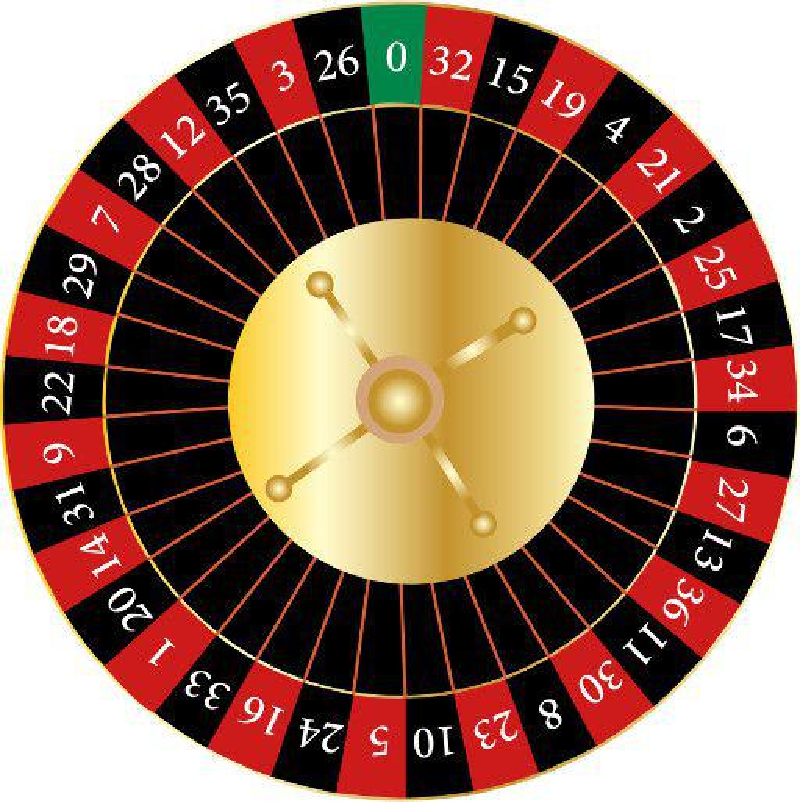
\includegraphics[width=0.75\textwidth]{figs/unit01_roulette.pdf}
\end{minipage}%
\begin{minipage}{0.5\textwidth}
  The standard European roulette wheel shown to the left (\href{https://www.vecteezy.com/vector-art/658761-casino-roulette-wheel}{source}) has 37 pockets labelled ``0'' through ``36''.
  18 of these pockets are coloured red, 18 are coloured black and 1 (pocket ``0'') is coloured green.
  Let an experiment be a spin of the roulette wheel, measuring the label of the pocket where the ball comes to rest (which also provides the pocket's colour).
\end{minipage}

\noindent What is the outcome space $A$ for a spin of the roulette wheel?
With $\cF = A$, what are the probabilities $p_{\al}$ for a fair wheel?
With
\begin{equation*}
  \cF = \left\{\mbox{ball in a red pocket, ball in a black pocket, ball in the green pocket}\right\},
\end{equation*}
what are the corresponding probabilities $p_{\text{red}}$, $p_{\text{black}}$ and $p_{\text{green}}$?
\begin{mdframed}
  \ \\[100 pt]
\end{mdframed}

The process of assigning probabilities to events is called \textit{modelling}.
The gaps above demonstrate that \textit{symmetries} are a powerful way to constrain probabilities.
The symmetry between the six sides of a fair die, the two sides of a fair coin, and the 37 pockets of a fair roulette wheel each sufficed to completely determine the corresponding probabilities $p_{\al}$.

Modelling can also be guided by empirical data obtained by repeating an experiment many times.
For example, if we don't know whether a set of dice are fair, we will be able to infer their probabilities $p_{\al}$ (with a certain confidence level) by rolling them enough times.
The need to repeat the experiment many times comes from the law of large numbers, to which we now turn.
% ------------------------------------------------------------------



% ------------------------------------------------------------------
\subsection{\label{sec:LLN}Law of large numbers}
Let's return to the setup leading to \eq{eq:finite_set} above, with
\begin{equation*}
  \cF = A = \left\{X_1, X_2, \cdots, X_n\right\}
\end{equation*}
for finite $n$, and probabilities $p_{\al} = P(X_{\al})$ that obey
\begin{align*}
  p_{\al} & \in [0, 1] &
  \sum_{\al = 1}^n p_{\al} & = 1.
\end{align*}
We can generalize this notation by writing instead
\begin{equation*}
  \sum_{X \in A} P(X) = 1,
\end{equation*}
and introducing similar expressions for the \textbf{mean} $\mu$ and \textbf{variance} $\si^2$ of the probability space,
\begin{align}
              \mu = \vev{X} = & \sum_{X \in A} X \, P(X)            \label{eq:mean} \\
  \si^2 = \vev{(X - \mu)^2} = & \sum_{X \in A} (X - \mu)^2 \, P(X). \label{eq:var}
\end{align}
The angle bracket notation indicates the \textbf{expected} (or \textbf{expectation}) \textbf{value} with general definition
\begin{equation}
  \label{eq:expect_disc}
  \vev{f(X)} = \sum_{X \in A} f(X) \, P(X),
\end{equation}
which is a linear operation,
\begin{equation*}
  \vev{c\cdot f(X) + g(X)} = c\vev{f(X)} + \vev{g(X)}.
\end{equation*}
The square root of the variance, $\sqrt{\si^2} = \si$, is the \textbf{standard deviation}.
What is \si expressed in terms of $\vev{X^2}$ and $\vev{X}^2$?
\begin{mdframed}
  \ \\[100 pt]
\end{mdframed}

We now define a new experiment that consists of \textit{repeating} the original experiment $R$ times, with each repetition independent of all the others.
Using the same measurement as before for each repetition, we obtain a new outcome space that we can call $B$.
For $R = 4$, what are some representative outcomes in the set $B$?
What is the total size of $B$?
\begin{mdframed}
  \ \\[100 pt]
\end{mdframed}

Each outcome in $B$ contains $R$ different $X^{(r)} \in A$, one for each repetition $r = 1, \cdots, R$, and each with mean $\vev{X^{(r)}} = \mu$ and variance $\vev{(X^{(r)} - \mu)^2} = \si^2$.
Considering the case $R = 4$ for simplicity, any element of $B$ can be written as $X_i^{(1)} X_j^{(2)} X_k^{(3)} X_l^{(4)} \in B$ with corresponding probability
\begin{equation*}
  P_B\left(X_i^{(1)} X_j^{(2)} X_k^{(3)} X_l^{(4)}\right) = P_A\left(X_i^{(1)}\right) P_A\left(X_j^{(2)}\right) P_A\left(X_k^{(3)}\right) P_A\left(X_l^{(4)}\right),
\end{equation*}
using subscripts to distinguish between the probability spaces for the single experiment ($A$) and repeated experiment ($B$).

Averaging over all $R$ repetitions defines the \textit{arithmetic mean}
\begin{equation}
  \label{eq:ave}
  \Xbar_R = \frac{1}{R} \sum_{r = 1}^R X^{(r)}.
\end{equation}
Unlike the true mean $\mu$, the arithmetic mean $\Xbar_R$ is a random variable --- a number that may be different for each element of $B$.
That said, $\Xbar_R$ and $\mu$ are certainly related, and so long as the standard deviation exists --- that is, so long as $\si^2$ is finite --- this relation can be proved rigorously in the limit $R \to \infty$.\footnote{In the computer project we will numerically investigate a situation where $\si^2$ diverges.}

Here we will not be fully rigorous, and take it as given that
\begin{equation*}
  \vev{\left(X^{(i)} - \mu\right)\left(X^{(j)} - \mu\right)} = \si^2 \de_{ij} = \left\{\begin{array}{ll}\si^2 & \mbox{for } i = j \\ 0 & \mbox{for } i \ne j\end{array}\right.,
\end{equation*}
where the \textit{Kronecker delta} $\de_{ij} = 1$ for $i = j$ and vanishes for $i \ne j$.
This is a consequence of our requirement that each repetition is independent of all the others.
Using this result and the relation $\big(\sum_i a_i\big)\big(\sum_j b_j\big) = \sum_{i, j} \left(a_i b_j\right)$, express the following quantity in terms of \si and $R$:
\begin{mdframed}
  $\displaystyle \vev{\left(\frac{1}{R} \sum_{r = 1}^R X^{(r)} - \mu\right)^2} = $ \\[200 pt]
\end{mdframed}
You should find that your result vanishes in the limit $R \to \infty$, so long as $\si^2$ is finite.
Since the square makes this expectation value a sum of non-negative terms, it can vanish only if every one of those terms is individually zero.

\begin{shaded}
  This establishes the \textbf{law of large numbers}:
  \begin{equation}
    \lim_{R \to \infty} \frac{1}{R} \sum_{r = 1}^R X^{(r)} = \mu,
  \end{equation}
  where we have assumed finite $\vev{X^{(r)}} = \mu$ and $\vev{(X^{(r)} - \mu)^2} = \si^2$.
\end{shaded}
% ------------------------------------------------------------------



% ------------------------------------------------------------------
\subsection{\label{sec:probdist}Probability distributions}
It is not necessary to make the assumption (\eq{eq:finite_set}) that our outcome space contains only a countable number of possible outcomes.
The considerations above continue to hold even if the random variable $X$ is a continuous real number.
In this case, however, the identification of probabilities with outcomes is slightly more complicated, which will be relevant when we consider the central limit theorem in the next section.

When the outcome can be any number on the real line, the fundamental object is a \textbf{probability distribution} (or \textbf{density function}) $p(x)$ defined for all $x \in \Rbb$.
Starting from this density, a probability is determined by integrating over a given interval.
Calling this interval $[a, b]$, the integration produces the probability that the outcome $X$ lies within the interval,
\begin{equation*}
  P\left(a \leq X \leq b\right) = \int_a^b p(x) \d{x}.
\end{equation*}

We similarly generalize the definition of an expectation value (\eq{eq:expect_disc}) to an integral over the entire domain of the  probability distribution,
\begin{equation*}
  \vev{f(x)} = \int f(x) \; p(x) \d{x}.
\end{equation*}
We will omit the limits on integrals over the entire domain, so for $x \in \Rbb$ we implicitly have $\int \d{x} = \int_{-\infty}^{\infty} \d{x}$, with $\int p(x) \d{x} = 1$.
An important set of expectation values is
\begin{equation}
  \label{eq:expect_cont}
  \vev{x^{\ell}} = \int x^{\ell} \; p(x) \d{x},
\end{equation}
which provides the mean and variance of the probability distribution $p(x)$, through generalizations of Eqs.~\ref{eq:mean}--\ref{eq:var}:
\begin{align}
  \label{eq:mean_var}
  \mu   & = \vev{x} = \int x \; p(x) \d{x} &
  \si^2 & = \vev{x^2} - \vev{x}^2.
\end{align}
The expression for the variance should be familiar from your determination of the standard deviation in an earlier gap.
Unless stated otherwise, we will assume the mean and variance are both finite for the probability distributions we consider.
% ------------------------------------------------------------------



% ------------------------------------------------------------------
\subsection{\label{sec:CLT}Central limit theorem}
The central limit theorem is a central result of probability theory (hence its name).
Over the years it has been expressed in several equivalent ways, and there are also many distinct variants of the theorem accommodating different conditions and assumptions.
Here we are interested in applying rather than proving the central limit theorem; you can find \href{https://en.wikipedia.org/wiki/Central_limit_theorem#Proof_of_classical_CLT}{proofs} in many textbooks.

The version of the theorem we use in this module assumes we have $N$ independent random variables $x_1, \cdots, x_N$, each of which has the same (finite) mean $\mu$ and variance $\si^2$.
Such random variables are said to be \textit{identically distributed}, and a common way to obtain them is to repeat an experiment $N$ times, as we considered in \secref{sec:LLN}.
Just as in \eq{eq:ave}, the sum
\begin{equation}
  \label{eq:CLTsum}
  s = \sum_{i = 1}^N x_i
\end{equation}
is itself a random variable.

\begin{shaded}
  The \textbf{central limit theorem} states that for large $N \gg 1$ the probability distribution for $s$ is
  \begin{equation}
    \label{eq:CLT}
    p(s) \approx \frac{1}{\sqrt{2\pi N\si^2}} \exp\left[-\frac{(s - N\mu)^2}{2N\si^2}\right],
  \end{equation}
  with the approximation becoming exact in the $N \to \infty$ limit.
\end{shaded}
In addition to asserting that the collective behaviour of many independent and identically distributed random variables $x_i$ is governed by a \textbf{normal} (or \textbf{gaussian}) \textbf{distribution}, the central limit theorem further specifies the precise form of this distribution in terms of the mean and variance of \textit{each individual} $x_i$. % TODO: Could explicitly emphasize connection to big picture of emergent phenomena...

\begin{minipage}{0.55\textwidth}
  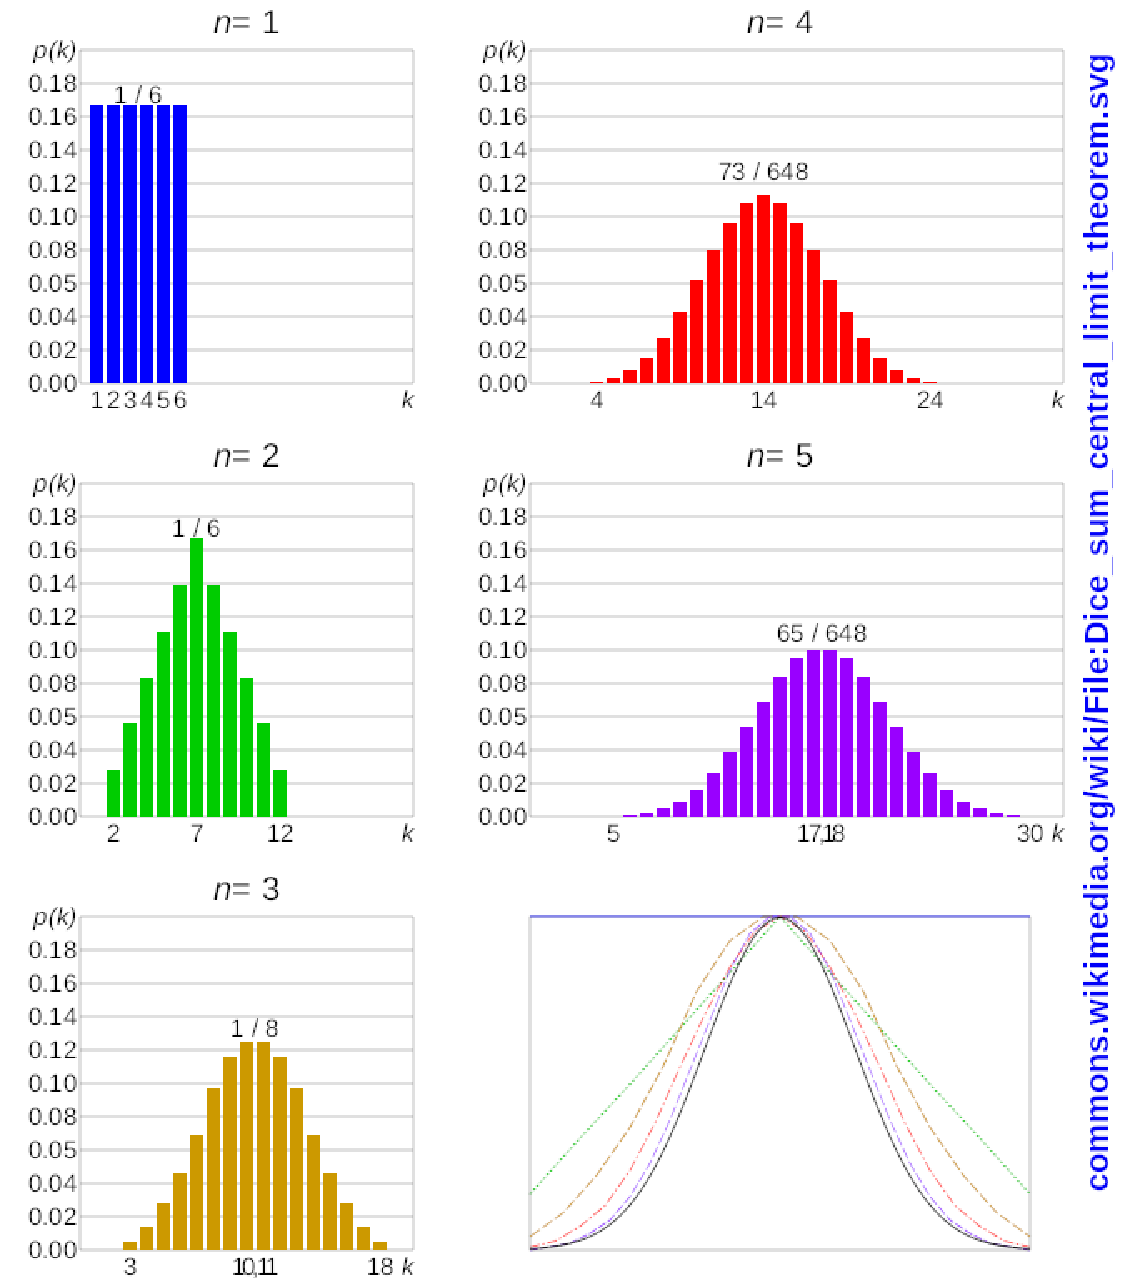
\includegraphics[width=0.8\textwidth]{figs/unit01_CLT.pdf}
\end{minipage}%
\begin{minipage}{0.35\textwidth}
  In practice, $N$ often doesn't need to be very large in order for the central limit theorem to provide a reasonable approximation.
  This is illustrated by the figure to the left, from \href{https://commons.wikimedia.org/wiki/File:Dice_sum_central_limit_theorem.svg}{{Wikimedia Commons}}, which shows the probabilities for the sum of $n \leq 5$ rolls of a six-sided die rapidly approaching a gaussian distribution.
\end{minipage}
% ------------------------------------------------------------------



% ------------------------------------------------------------------
\subsection{\label{sec:diffusion}Diffusion and the central limit theorem}
\subsubsection{Random walk on a line}
As a more powerful application and illustration of the central limit theorem, let's consider the behaviour of a randomly moving object.
Such \textbf{random walks} appear frequently in mathematical modelling of stochastic phenomena (including Brownian motion), and can be applied to movement through either physical space or more abstract vector spaces.
They are examples of \href{https://en.wikipedia.org/wiki/Markov_process}{Markov processes}, in which the state of the system (in this case the position of the `walker') at any time probabilistically depends only on the system's prior state at the previous point in time --- there is no `memory' of any earlier states. % Named after \href{https://en.wikipedia.org/wiki/Andrey_Markov}{Andrey Markov}...
The resulting sequence of system states is known as a \textit{Markov chain}, since each state is produced from the one before, like links in a chain. % ``system state'' later mentioned as synonym for macro-state...

Let's consider the simple example of a random walker that moves only in a single spatial dimension --- to the left or to the right on a line --- and can only take `steps' of a fixed length, which we can set to $\ell = 1$ without loss of generality.
At each point in time, the walker takes either a step to the right ($R$) with probability $p$ or a step to the left ($L$) with probability $q = 1 - p$.
We will further assume that each step takes a constant amount of time $\de t$, so a walk of $N$ steps will last for total time
\begin{equation}
  \label{eq:RWtime}
  t = N \de t.
\end{equation}

As an example, for $N = 6$ a representative walk can be written as $LRLRRR$, which leaves the walker $x = 2$ steps to the right of its starting point ($x = 0$).
The opposite walk $RLRLLL$ would leave the walker at $x = -2$, with negative numbers indicating positions to the left of the starting point.
How many possible walks are there for $N = 6$, and what is the probability (in terms of $p$ and $q$) for the walks $LRLRRR$ and $RLRLLL$ to occur?
How many possible walks are there for general $N$, and what is the probability for any particular walk involving $r$ steps to the right to occur?
\begin{mdframed}
  \ \\[80 pt]
\end{mdframed}

We are interested in the walker's final position $x$ at time $t$ after it has taken $N$ steps.
Just as for the sum of $n$ rolls of a die considered in \secref{sec:CLT}, there are a range of possible final positions $x$, each of which has some probability $P(x)$ of being realized.
The key pieces of information we want to determine are the expectation value $\vev{x}$ and the standard deviation $\De x \equiv \sqrt{\vev{x^2} - \vev{x}^2}$ that indicates the scale of fluctuations we can expect around $\vev{x}$ as the $N$-step walk is repeated many times from the same starting point.
(We reserve the variables $\mu$ and $\si^2$ for the mean and variance \textit{of the single-step process}, which will play an important role when we apply the central limit theorem in \secref{sec:RW_CLT}.)

Suppose the $N$ total steps involve $r$ steps to the right.
What is the final position $x$ of the walker in terms of $N$ and $r$?
Check your general answer for the cases $N = 6$ and $r = 4$, $2$ considered above.
\begin{mdframed}
  \ \\[100 pt]
\end{mdframed}
This relation makes it equivalent to consider either the probability $P_r$ of taking $r$ steps to the right, or the probability $P(x)$ of ending up at final position $x$.
This equivalence \textbf{will not hold} for more general random walks in which the step length is no longer fixed and $\ell_i$ can vary from one step to the next.

Because the order in which steps are taken does not affect the final position $x$, to determine the probability $P(x)$ we have to count all possible ways of walking to $x$.
For $N = 6$, what are all the possible walks that produce $x = 4$, and what is the corresponding probability $P(4)$?
\begin{mdframed}
  \ \\[100 pt]
\end{mdframed}
Your answer should have a factor of $6$ that corresponds to the binomial coefficient $\binom{N}{r} = \binom{6}{5} = 6$.
In terms of this binomial coefficient, what is the general probability $P_r$ that an $N$-step walk will include $r$ steps to the right in any order?
\begin{mdframed}
  \ \\[100 pt]
\end{mdframed}
% TODO: This is the \href{https://en.wikipedia.org/wiki/Binomial_distribution}{binomial distribution}, which students sometimes look up and (mis)use on their own...

\newpage % WARNING: FORMATTING BY HAND
Given this probability $P_r$, we can apply Eqs.~\ref{eq:mean}--\ref{eq:var} to find the expectation value $\vev{x}$ and the standard deviation $\De x$.
As a first step, what are $\vev{x}$ and $\vev{x^2}$ in terms of the expectation values $\displaystyle \vev{r^n} = \sum_{r = 0}^N r^n \, P_r$?
\begin{mdframed}
  $\vev{x}   = $ \\[50 pt]
  $\vev{x^2} = $ \\[50 pt]
\end{mdframed}
Now we need to calculate the necessary $\vev{r^n}$.
A powerful way to do this is to define the \textbf{generating function}
\begin{equation}
  G(\theta) = \sum_{r = 0}^N e^{r \theta} \, P_r.
\end{equation}
This approach introduces a parameter $\theta$ that we subsequently remove by setting $\theta = 0$.
For example, $G(0) = \sum_{r = 0}^N P_r = 1$.
What do you obtain upon taking derivatives of the generating function and then setting $\theta = 0$?
\begin{mdframed}
  $\displaystyle \left.\frac{d}{d\theta} G(\theta)\right|_{\theta = 0} = $ \\[50 pt]
  $\displaystyle \left.\frac{d^n}{d\theta^n} G(\theta)\right|_{\theta = 0} = $ \\[50 pt]
\end{mdframed}

For the current case of a fixed-step-length random walk in one dimension, the probabilities $P_r$ produce a simple closed-form expression for the generating functional:
\begin{equation}
  \label{eq:gen_func}
  G(\theta) = \sum_{r = 0}^N e^{r \theta} \, P_r = \sum_{r = 0}^N e^{r \theta} \binom{N}{r} p^r q^{N - r} = \left(e^{\theta} p + q\right)^N,
\end{equation}
making use of the binomial formula $\left(a + b\right)^N = \sum_{i = 0}^N \binom{N}{i} a^i b^{N - i}$.

\newpage % WARNING: FORMATTING BY HAND
It's straightforward to take the necessary derivatives of \eq{eq:gen_func}, which simplify pleasantly since $\left.\left(e^{\theta} p + q\right) \right|_{\theta = 0} = p + q = 1$:
\begin{mdframed}
  $\displaystyle \left.\frac{d}{d\theta} \left(e^{\theta} p + q\right)^N \right|_{\theta = 0} = $ \\[50 pt]
  $\displaystyle \left.\frac{d^2}{d\theta^2} \left(e^{\theta} p + q\right)^N \right|_{\theta = 0} = $ \\[75 pt]
\end{mdframed}
Insert the resulting $\vev{r}$ and $\vev{r^2}$ into the relations derived above:
\begin{mdframed}
  $\vev{x} = $ \\[50 pt]
  $(\De x)^2 = \vev{x^2} - \vev{x}^2 = $ \\[50 pt]
\end{mdframed}
In the end, you should obtain % TODO: The computations in this subsection might work well as a tutorial activity...
\begin{align}
  \label{eq:RWmean}
  \vev{x} & = N(2p - 1) &
  \De x & = 2\sqrt{Npq}.
\end{align}
We can check that this $\vev{x}$ produces the expected results in the special cases $p = 0$, $1 / 2$ and $1$, while the standard deviation $\De x$ also behaves appropriately by vanishing for both $p = 0$ and $1$.
% ------------------------------------------------------------------



% ------------------------------------------------------------------
\subsubsection{Law of diffusion}
It's possible to interpret the results in \eq{eq:RWmean} in a more intuitive way by expressing them in terms of the total time $t$ taken by the random walk (\eq{eq:RWtime}).
Inserting $N = t / \de t$ into \eq{eq:RWmean},
\begin{equation*}
  \vev{x} = \frac{t}{\de t} (2p - 1) = \frac{2p - 1}{\de t} t \equiv \vdr t,
\end{equation*}
we see that the \textit{expected} final position of the walker depends linearly on time, with \textbf{drift velocity}
\begin{equation}
  \vdr = \frac{2p - 1}{\de t} = \frac{N(2p - 1)}{t} = \frac{\vev{x}}{t}.
\end{equation}
The sign of \vdr indicates whether the walker is drifting to the right ($p > \frac{1}{2}$) or to the left ($p < \frac{1}{2}$).
The typical scale of fluctuations (or the `uncertainty') around the expected final position $\vev{x}$ is given by the standard deviation $\De x$, and also depends on time:
\begin{equation*}
  \De x = \sqrt{\vev{x^2} - \vev{x}^2} = 2\sqrt{Npq} = 2\sqrt{\frac{pq}{\de t}} \sqrt{t},
\end{equation*}
where the constant factor is non-negative.
This $\sqrt{t}$ dependence is a very general result.

\begin{shaded}
  The \textbf{law of diffusion} states that
  \begin{equation}
    \label{eq:diff_law}
    \De x = D \sqrt{t},
  \end{equation}
  where $D > 0$ is the \textbf{diffusion constant}.
  The standard deviation $\De x$ is sometimes also called the \textit{diffusion length}.
\end{shaded}

The result $D = 2\sqrt{\frac{pq}{\de t}}$ that we computed above is specific to the simple example of a fixed-step-length random walk in one dimension and \textbf{will not hold} for more general random walks.
The behaviour it describes is illustrated by the figure below, which plots the $t$-dependent probability distribution $p(x)$ that we'll soon derive using the central limit theorem (\eq{eq:RW_CLT}).
What we can see already, even before completing that derivation, is that the probability distribution steadily spreads out --- or \textit{diffuses} --- as time passes:
\begin{center}
  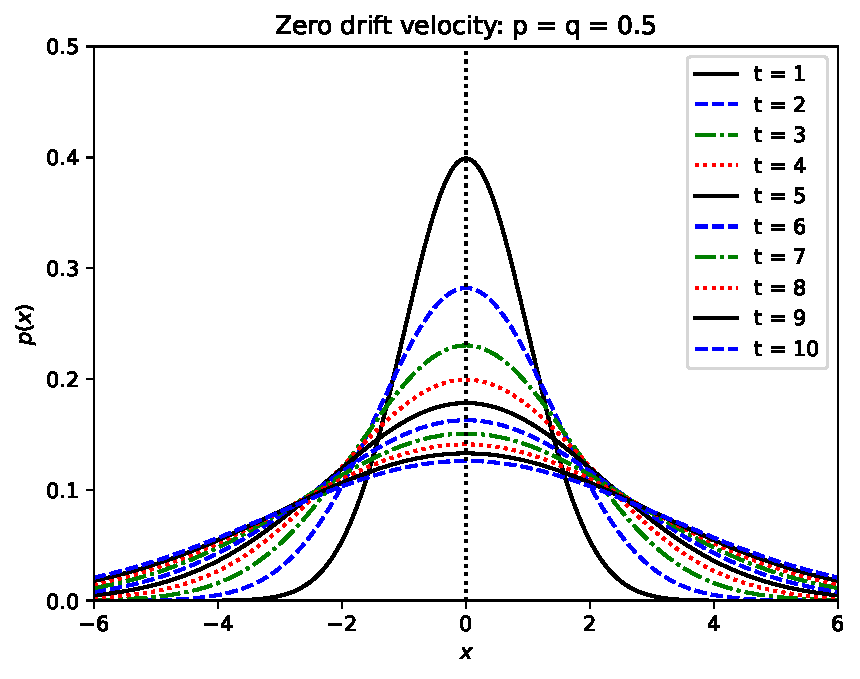
\includegraphics[width=0.6\textwidth]{figs/unit01_diff_zero.pdf} % WARNING: ADJUSTED BY HAND TO OPTIMIZE PAGE BREAK
\end{center}
Here we are considering the special case $p = q = \frac{1}{2}$, for which the drift velocity $\vdr = 0$ and the expectation value is always $\vev{x} = 0$ for any walk time $t$.
However, as time goes on, there is a steady decrease in the probability that the walker will end up around its starting point $x \approx 0$.
(As described in \secref{sec:probdist}, we can determine this probability by integrating the distribution $p(x)$ over an appropriate interval.)
Instead, the interval $-D\sqrt{t} \leq x \leq D\sqrt{t}$ within which we can expect to find the walker (with a constant `one-sigma' or $\sim$68\% probability) steadily grows with characteristic dependence on the square root of the time the diffusive process lasts.

Except in the trivial cases $p = 0$ or $q = 0$, diffusion also occurs when the drift velocity is non-zero.
This is shown in the two figures below, considering a low but non-zero drift velocity $\vdr = 0.2$ on the left, and a high $\vdr = 0.98$ on the right.
All three figures were produced by \href{https://github.com/daschaich/MATH327_2025/blob/main/lecture_notes/unit01_dist.py}{this Python script}.
\begin{center} % Don't need centering, but this will provide consistent vertical spacing
  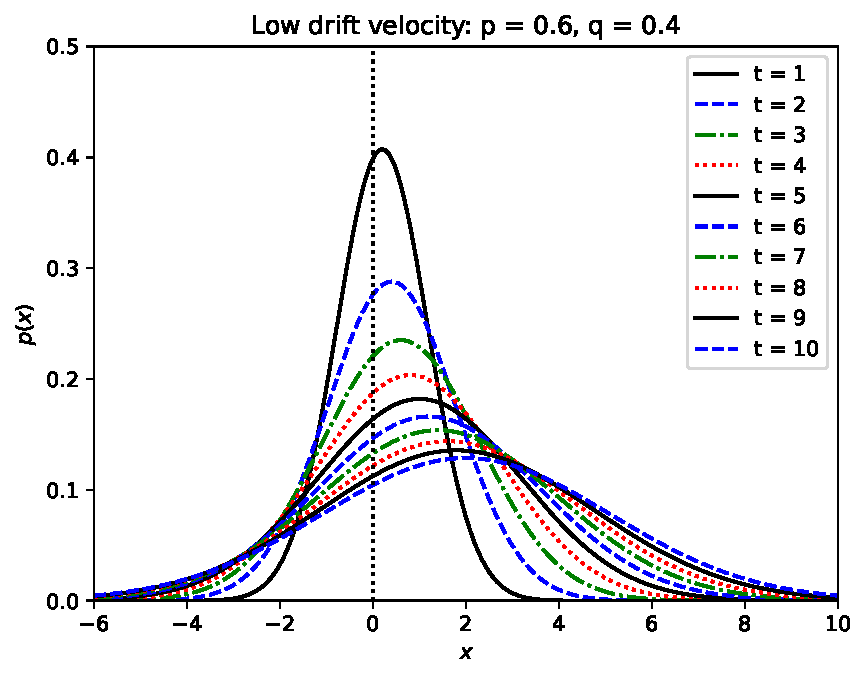
\includegraphics[width=0.475\textwidth]{figs/unit01_diff_low.pdf}\hfill 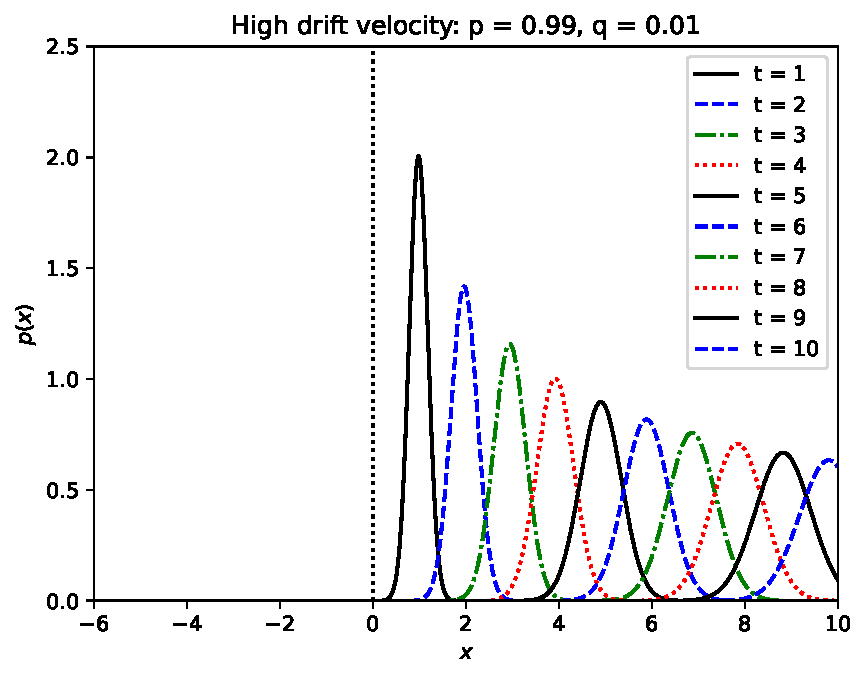
\includegraphics[width=0.475\textwidth]{figs/unit01_diff_high.pdf}
\end{center}
In the figure on the left, the large diffusion constant $D \approx 0.980$ produces a plot that looks similar to the $\vdr = 0$ case on the previous page, but now the central peaks (and expectation values $\vev{x}$) for each $t$ drift steadily to the right.
The lower $D \approx 0.199$ for the figure on the right leads to less overlap among the distributions, but they still diffuse to exhibit lower and broader peaks as time passes.

When $p \neq \frac{1}{2}$ so that $\vev{x} \neq 0$, it is interesting to compare the drift in the expectation value against the growth in fluctuations around $\vev{x}$ due to diffusion.
We can do this by considering the following \textit{relative} uncertainty:
\begin{mdframed}
  $\frac{\De x}{\vev{x}} = $ \\[100 pt]
\end{mdframed}
You should find that at large times this ratio vanishes proportionally to $1 / \sqrt{t} \propto 1 / \sqrt{N}$.
Although the absolute uncertainty $\De x = D \sqrt{t}$ grows by diffusion, for $\vdr \neq 0$ the linear drift in the expectation value becomes increasingly dominant as time goes on.
% ------------------------------------------------------------------



% ------------------------------------------------------------------
\newpage % WARNING: FORMATTING BY HAND
\subsubsection{\label{sec:RW_CLT}Applying the central limit theorem}
Based on our work in \secref{sec:CLT}, we can see how to apply the central limit theorem to analyse this fixed-step-length random walk in one dimension, for large numbers of steps $N$ or equivalently large times $t = N \de t$.
Each step in the random walk is an independent and identically distributed random variable $x_i$.
The corresponding probability space involves only two possible outcomes: a step of length $\ell = 1$ to the right or to the left with probability $p$ or $q$, respectively.
From this we can easily compute the mean and variance \textit{of the single-step process}:
\begin{mdframed}
  $\mu = \vev{x_i} = $ \\[33 pt]
  $\vev{x_i^2} = $ \\[33 pt]
  $\si^2 = \vev{x_i^2} - \vev{x_i}^2 = $ \\[30 pt]
\end{mdframed}

The final position $x$ of the walker after $N$ steps is exactly the sum over these $x_i$ given in \eq{eq:CLTsum}.
Its probability distribution $p(x)$ from the central limit theorem is therefore obtained directly from these single-step $\mu$ and $\si^2$, which we can also express in terms of the drift velocity and diffusion constant:
\begin{align}
  p(x) & = \frac{1}{\sqrt{2\pi (4Npq)}} \exp\left[-\frac{(x - N(2p - 1))^2}{8Npq}\right] \cr
       & = \frac{1}{\sqrt{2\pi D^2 t}} \exp\left[-\frac{(x - \vdr t)^2}{2D^2 t}\right]. \label{eq:RW_CLT}
\end{align}
This expression was used to produce the three figures above.
We could have jumped straight to the final line by considering \eq{eq:CLT} and noting
\begin{align}
  \label{eq:single_step}
  \vdr t & = N(2p - 1) = N \mu &
  D^2 t & = 4pq \frac{t}{\de t} = N \si^2.
\end{align}
While this dependence on $p$ and $q$ is specific to the particular fixed-step-length random walk we're currently considering, the generic results $\vdr t = N \mu$ and $D^2 t = N \si^2$ in \eq{eq:single_step} \textbf{do hold} for any random walk with finite $\mu$ and $\si^2$ (so that the central limit theorem can be applied).
This is remarkable, because it means that the diffusive process as a whole is determined entirely by the single-step mean and variance.
So long as $\mu$ and $\si^2$ are finite, we end up with \eq{eq:RW_CLT} as the large-$t$ probability distribution for any markovian random walk in a single variable $x$.

This result is related to the generality of the law of diffusion (\eq{eq:diff_law}), which we can recognize in the structure of \eq{eq:RW_CLT}.
Since $t > 0$, the exponential in the gaussian distribution $p(x)$ peaks at the drifting expectation value $x = \vdr t = \vev{x}$.
The factor $(x - \vdr t)^2$ simply quantifies the distance from this peak.
As $t$ increases, so does the factor $2D^2 t$ dividing this $(x - \vdr t)^2$, meaning that a larger distance from the peak is needed for the overall argument of the exponential to reach a given value --- in other words, the peak becomes broader.
This in turn requires a lower peak, reflected in the $\frac{1}{\sqrt{t}}$ in the overall coefficient, which is set by requiring $\int p(x) \d{x} = 1$.
In other words, the law of diffusion holds whenever the central limit theorem is applicable.
This requires that the mean and variance of the single-step process are finite, and in the computer project we will numerically investigate the \textit{anomalous diffusion} that occurs when this condition is not satisfied.
% ------------------------------------------------------------------


\newpage
% ------------------------------------------------------------------
\renewcommand{\thisunit}{MATH327 Unit 2}
\renewcommand{\moddate}{Last modified 2 Feb.~2025}
\setcounter{section}{2}
\setcounter{subsection}{0}
\phantomsection
\addcontentsline{toc}{section}{Unit 2: Micro-canonical ensemble}
\section*{Unit 2: Micro-canonical ensemble}
\subsection{\label{sec:ensemble}Statistical ensembles and thermodynamic equilibrium}
We begin this unit by establishing the concept of \textit{statistical ensembles}, which was formalized by \href{https://en.wikipedia.org/wiki/Josiah_Willard_Gibbs}{J.\ Willard Gibbs} in 1902. % en.wikipedia.org/wiki/Ensemble_(mathematical_physics)
(Gibbs also introduced the term `statistical mechanics', in 1884.)
Building on the probability foundations laid above, we will be interested in `experiments' that simply allow a collection of degrees of freedom to evolve in time, subject to certain constraints.
At a given time $t_1$, the arrangement of these degrees of freedom defines the state $\om_1$ of the system.

As a concrete example, consider a system of \textit{spins} --- arrows that can point either `up' or `down' --- arranged in a line.
Such \href{https://en.wikipedia.org/wiki/Spin_model}{spin systems} will appear several times in the remainder of this module, since in addition to obeying simple mathematics analogous to flipping coins, spins also serve as good models of physical systems such as magnetic molecules.
What would be a representative state (or \textit{configuration}) for a system of $N = 8$ spins?
How many distinct states are there for this system?
\begin{mdframed}
  \ \\[80 pt]
\end{mdframed}

At a different time $t_2$, the system's state $\om_2$ is generally different from $\om_1$.
However, there are some measurements we can perform that always produce the same outcome even as the system's state changes over time.
These measurements define \textit{conserved quantities}, such as the number of spins considered in the example above.

Another important conserved quantity is the \textit{internal} energy $E$ of an isolated (or `closed') system,
\begin{equation*}
  E(\om_1) = E(\om_2).
\end{equation*}
The conservation of energy is presumably a familiar concept, and you may also know that it can be rigorously proven through \href{https://en.wikipedia.org/wiki/Emmy_Noether}{Emmy Noether}'s \href{https://en.wikipedia.org/wiki/Noether's_theorem}{first theorem}.\footnote{There are \href{https://www.preposterousuniverse.com/blog/2010/02/22/energy-is-not-conserved/}{complications} when considering the dynamical space-time of general relativity, but that's beyond the scope of this module.}
Because conservation of energy was empirically observed long before Noether's theorem was proven, it also has a more grandiose name: the \textbf{first law of thermodynamics}.
Another way of stating the first law is that any change in the internal energy of one particular system \Om must be matched by an equal and opposite change in the energy of some other system with which \Om is in contact.
This will be important when we consider thermodynamic cycles later in the term.

For now, let's return to the example above, and endow the spin system with an internal energy by placing it in a `magnetic field' of strength $H$.
That is, if a spin is parallel to the field, it contributes energy $-H$ to the total energy $E$ of the system. % mu_B=1 in natural units
If a spin is anti-parallel to the field, it instead contributes energy $H$.
For later convenience, we define a positive magnetic field $H > 0$ to point upward, and also define $n_+$ to be the number of spins pointing upward --- parallel to the field and therefore contributing \textit{negative} energy.
Similarly, the remaining $n_- = N - n_+$ downward-pointing spins are anti-parallel to the field and contribute positive energy.
What is the total energy $E$ of the system in terms of $n_+$ and $n_-$?
What is $E$ for the representative $8$-spin state you wrote down above?
What fraction of the states of the spin system have this energy?
\begin{mdframed}
  \ \\[100 pt]
\end{mdframed}

If instead we consider $N \sim 10^{23}$ hydrogen (H$_2$) molecules in a container, we can write a simple expression for the internal energy $E$ by treating each molecule as a \textit{point-like particle}, with no size or structure.
In this case each molecule contributes only its kinetic energy, and
\begin{equation*}
  E = \frac{m}{2} \sum_{n = 1}^N \vec{v}_n^{\,2} = \frac{1}{2m} \sum_{n = 1}^N \vec{p}_n^{\,2},
\end{equation*}
where $\vec v_n$ is the velocity of the $n$th molecule, $\vec p_n = m \vec v_n$ is its momentum, and all molecules have the same mass $m$.

As forecast at the start of the module, we treat the time evolution of any given system as a stochastic process in which the system probabilistically adopts a sequence of states $\om_i \in \Om$:
\begin{equation*}
  \om_1 \lra \om_2 \lra \om_3 \lra \om_4 \lra \cdots
\end{equation*}
This approach is a matter of practicality rather than one of principle.
In principle, Newton's laws would allow us to predict the exact time evolution of (say) $10^{23}$ hydrogen molecules, but only by specifying $10^{23}$ initial conditions and solving $10^{23}$ differential equations.
Since we cannot hope to record so much information or carry out so many computations, we instead apply probability theory in order to analyse these systems.

\begin{shaded}
  This leads us to the following core definition: A \textbf{statistical ensemble} is the set of all states $\Om = \left\{\om_1, \om_2, \cdots\right\}$ that a system can possibly adopt through its time evolution.
  Each state $\om_i$ has some probability $p_i$ of being adopted by the system, so we can recognize a statistical ensemble as a probability space. % State space as outcome space in unit 1
\end{shaded}

Because these states $\om_i$ depend on the `microscopic' degrees of freedom that compose the overall system, we will refer to them as \textbf{micro-states} from now on.
From the definition of probability in \secref{sec:prob}, we have the requirement $\sum_i p_i = 1$, which simply means that the system must be in \textit{some} micro-state at any point in time.
The fact that time evolution cannot change any conserved quantities, as discussed above, means that such conserved quantities characterize statistical ensembles.
Throughout the next seven units we will consider different statistical ensembles with different sets of conserved quantities.

\begin{shaded}
  First we define the \textbf{micro-canonical ensemble} to be a statistical ensemble characterized by conserved internal energy $E$ and conserved number of degrees of freedom $N$ --- which we will call \textbf{particle number} for short.
\end{shaded}

According to the discussion above, this means that a system governed by the micro-canonical ensemble is \textit{isolated} in the sense that it cannot exchange energy or particles with any other system.

Now that the micro-canonical ensemble is defined, we can connect it to our intuition from everyday physical systems.
Let's consider a collection of particles moving around and bouncing (or `\textit{scattering}') off each other in a sealed container.
To a first approximation, this should describe the behaviour of air in a room, which our lived experience indicates is spread quite uniformly throughout the room in a way that is stable as time passes.
We do not expect all the air in a room to be concentrated in any one corner, nor do we expect strong collective gusts of wind without some clear external influence.

These qualitative expectations illustrate the idea of \textbf{thermodynamic equilibrium}, an axiomatic concept in statistical mechanics.\footnote{Our expectation that physical systems generically evolve towards thermodynamic equilibrium as time passes is more formally expressed as the \href{https://en.wikipedia.org/wiki/Ergodic_hypothesis}{ergodic hypothesis}.}
We can mathematically define thermodynamic equilibrium through the probabilities $p_i$ that appear in the micro-canonical ensemble.

\begin{shaded}
  A micro-canonical system \Om with $M$ micro-states $\om_i$ is in thermodynamic equilibrium if and only if all probabilities $p_i$ are equal.
  If $M$ is finite, the requirement $\sum_i p_i = 1$ implies
  \begin{equation}
    \label{eq:micro_equil}
    p_i = \frac{1}{M}.
  \end{equation}
\end{shaded}

The full meaning and significance of this definition are not immediately obvious, and we will continue exploring them through consideration of derived quantities such as entropy and temperature.
First, it's important to emphasize that this equilibrium is \textit{dynamic}: There is not a single `equilibrium micro-state' that the system sits in.
Instead, the equilibrium system continues probabilistically adopting all possible micro-states as it evolves in time. % In the micro-canonical case, all accessible micro-states have the same energy and particle number, but this concept of (dynamic) thermodynamic equilibrium will generalize...
% ------------------------------------------------------------------



% ------------------------------------------------------------------
\subsection{\label{sec:entropy}Entropy and its properties}
\subsubsection{Definition of entropy}
We can gain further insight into thermodynamic equilibrium by considering a famous derived quantity.
\begin{shaded}
  The \textbf{entropy} of a statistical ensemble \Om with a countable number of micro-states $M$ is defined to be
  \begin{equation}
    \label{eq:entropy}
    S = - \sum_{i = 1}^M p_i \log p_i,
  \end{equation}
  where $p_i$ is the probability for micro-state $\om_i$ to occur.
  Unless otherwise specified, ``$\log$'' indicates the natural logarithm with base $e$.
\end{shaded}

When the system under consideration is in thermodynamic equilibrium, we expect derived quantities such as the entropy to be stable over time, even as different micro-states are probabilistically adopted.
This implies that such derived quantities are functions of the conserved quantities that are the same for all micro-states.
Therefore, for the micro-canonical ensemble, the equilibrium entropy $S(E, N)$ is a function of the conserved energy and particle number.

By inserting \eq{eq:micro_equil} into \eq{eq:entropy} you can quickly compute a simple expression for the entropy of a micro-canonical ensemble in thermodynamic equilibrium:
\begin{mdframed}
  \ \\[40 pt]
\end{mdframed}
Your result should depend only on the number of micro-states $M$, diverging as $M \to \infty$.
While the energy $E$ and particle number $N$ are not explicit in this expression, $\left\{E, N, M\right\}$ are inter-related and can be expressed in terms of each other given the details of any specific situation under consideration.
For example, what is the equilibrium entropy of the system of $N$ spins considered above, if the magnetic field is turned off, $H = 0$?
What is the entropy if $E = 0$ with $H > 0$ (which requires $n_+ = n_-$)?
\begin{mdframed}
  \ \\[110 pt]
\end{mdframed}
% ------------------------------------------------------------------



% ------------------------------------------------------------------
\subsubsection{Extensivity}
The increase in entropy for an increasing number of micro-states $M$ is a reflection of entropy being an \textit{extensive} quantity.
Extensive quantities are formally defined by considering how they behave if two isolated subsystems are \textit{analysed} as a single system --- while still remaining isolated from each other, exchanging neither energy nor particles.
This is clearest to consider through the specific example shown below of two isolated spin subsystems, $\Om_1$ \& $\Om_2$, characterized by the energies $E_1$ \& $E_2$ and particle numbers $N_1$ \& $N_2$, respectively.
To simplify the subsequent analysis, we can assume that both subsystems are placed in magnetic fields with the same $H$, so that $E_S = -H\left(n_+^{(S)} - n_-^{(S)}\right)$ for $S \in \left\{1, 2\right\}$.
\begin{center}
  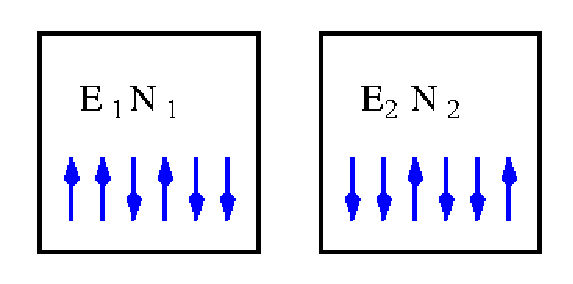
\includegraphics[width=0.7\textwidth]{figs/unit02_entropy-separate.pdf}
\end{center}

We can take system $\Om_1$ to have $M_1$ micro-states with probabilities $p_i$ while system $\Om_2$ has $M_2$ micro-states with probabilities $q_k$.
As discussed above, each $M_S$ is determined by $E_S$ and $N_S$.
The entropies of the two systems are
\begin{align*}
  S_1 & = - \sum_{i = 1}^{M_1} p_i \log p_i &
  S_2 & = - \sum_{k = 1}^{M_2} q_k \log q_k.
\end{align*}

\begin{center}
  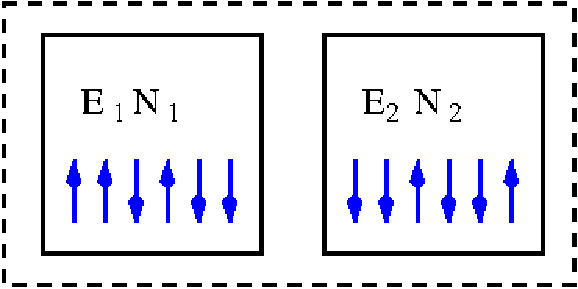
\includegraphics[width=0.7\textwidth]{figs/unit02_entropy-combo.pdf}
\end{center}

Now we keep these two subsystems isolated from each other, but consider them as a combined system $\Om_{1+2}$, as illustrated above.
In order to compute the entropy $S_{1+2}$, we need to figure out the number of micro-states $M_{1+2}$ the combined system could possibly adopt, and then determine the corresponding probability for each micro-state.
Both steps are simplified by the subsystems being isolated from each other, so that they are statistically independent.
Specifically, with subsystem $\Om_1$ in any one of its $M_1$ micro-states $\om_i^{(1)}$, subsystem $\Om_2$ could independently adopt any of its $M_2$ micro-states, implying $M_{1+2} = M_1 M_2$.

Similarly, statistical independence means that the combined probability of subsystem $\Om_1$ adopting micro-state $\om_i^{(1)}$ while subsystem $\Om_2$ adopts $\om_k^{(2)}$ is the product of the individual probabilities, $p_i q_k$.
We can check this is a well-defined probability, with
\begin{equation*}
  \sum_{M_{1+2}} p_i q_k = \sum_{i = 1}^{M_1} \sum_{k = 1}^{M_2} p_i q_k = \left[\sum_{i = 1}^{M_1} p_i\right]\cdot \left[\sum_{k = 1}^{M_2} q_k\right] = 1\cdot 1 = 1.
\end{equation*}
Inserting the probability $p_i q_k$ into \eq{eq:entropy}, and recalling $\log(a\cdot b) = \log a + \log b$, what is the combined entropy $S_{1+2}$ of these two independent subsystems?
\begin{mdframed}
  $S_{1+2} = $ \\[100 pt]
\end{mdframed}
You should find that the total entropy is the sum of the entropies of the two isolated subsystems, which is also how the energies and particle numbers behave,
\begin{align*}
  E_{1+2} & = E_1 + E_2 &
  N_{1+2} & = N_1 + N_2.
\end{align*}

This behaviour identifies the energy, particle number and entropy as \textbf{extensive} quantities, which are \href{https://goldbook.iupac.org/terms/view/E02281}{defined} to be those that add up across independent subsystems.
This can be contrasted with \textbf{intensive} quantities, which are \href{https://goldbook.iupac.org/terms/view/I03074}{defined} to be independent of the extent of the system, and hence the same (on average) for subsystems as for the combined system. % External magnetic field strength $H$ is control parameter rather than system property --- will be formally introduced in Unit 4
Temperature and density are everyday examples of intensive quantities, though we will see below that the micro-canonical approach introduces some subtleties.
It is possible for quantities to be neither extensive nor intensive, for example the number of micro-states $M_{1+2} = M_1 M_2$.

Finally, suppose that each subsystem is independently in thermodynamic equilibrium, with finite $M_1$ and $M_2$, implying
\begin{align*}
  p_i & = \frac{1}{M_1} & q_k & = \frac{1}{M_2} \\
  S_1 & = \log M_1      & S_2 & = \log M_2.
\end{align*}
As a consequence we can establish that $\Om_{1+2}$ is also in thermodynamic equilibrium, since the probabilities
\begin{equation*}
  p_i q_k = \frac{1}{M_1 M_2} = \frac{1}{M_{1+2}}
\end{equation*}
are identical all of its micro-states.
In this situation it's even easier to see $S_{1+2} = \log\left(M_1 M_2\right) = \log M_1 + \log M_2 = S_1 + S_2$.
% ------------------------------------------------------------------



% ------------------------------------------------------------------
\subsubsection{\label{sec:second_law}Second law of thermodynamics}
Let's continue considering two subsystems, with one significant change: Suppose the subsystems are now able to exchange energy (but not particles) with each other.
We'll say they are in \textit{thermal contact} with each other, rather than being fully isolated.
We'll also wait long enough after establishing thermal contact for the combined system \Om to reach equilibrium.
This is illustrated below:
\begin{center}
  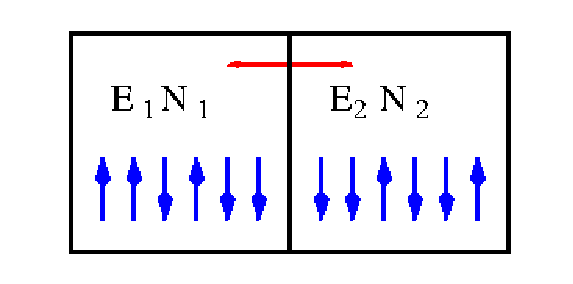
\includegraphics[width=0.7\textwidth]{figs/unit02_entropy-exchange.pdf}
\end{center}
The total energy $E = E_1 + E_2$ remains conserved, so the overall system \Om is still governed by the micro-canonical ensemble.
However, the individual energies $E_1$ and $E_2$ can now change over time, meaning that \textit{each subsystem is no longer micro-canonical}.

The overall system \Om is \textit{not} the same as the combined $\Om_{1+2}$ considered above.
We need to reconsider the total number of micro-states $M$ that \Om could adopt, which is much more difficult than before because we can no longer apply statistical independence.
Our key remaining tool is the conservation of the total energy $E$.

Considering a micro-state in which the $N_1$ spins contribute energy $e_1$ to the total, we know that the $N_2$ spins must contribute the remaining $E - e_1$.
Our work above implies there are $M_{e_1} = M_{e_1}^{(1)} M_{E - e_1}^{(2)}$ micro-states providing this particular distribution of energies, where $M_{e_1}^{(1)}$ is the number of micro-states of the formerly isolated subsystem $\Om_1$ with energy $e_1$, and $M_{E - e_1}^{(2)}$ similarly corresponds to $\Om_2$ with energy $E - e_1$.
We also know that it's possible to have $e_1 = E_1$, since that's the initial energy of $\Om_1$ before it was brought into thermal contact with $\Om_2$.
When $e_1 = E_1$, we have $M_{E_1} = M_1 M_2$, covering all the micro-states of the combined $\Om_{1+2}$ when the two subsystems were isolated.
\textit{In addition}, we also have to count any other micro-states for which $e_1 \ne E_1$:
\begin{equation}
  \label{eq:micro_sum}
  M = \sum_{e_1} M_{e_1}^{(1)} M_{E - e_1}^{(2)} = M_1 M_2 + \sum_{e_1 \ne E_1} M_{e_1}^{(1)} M_{E - e_1}^{(2)} \geq M_1 M_2.
\end{equation}
Equality holds when $e_1 = E_1$ is the only possibility --- this is an extremely special case, in which the two subsystems remain individually micro-canonical, with fixed $E_1$ and $E_2$.
This is all we can say in full generality, without specifying more details of a particular example, but it allows us to obtain a famous result for the total entropy $S$ of \Om \textit{in thermodynamic equilibrium}:
\begin{equation*}
  S = \log M \geq \log\left(M_1 M_2\right) = S_{1+2}.
\end{equation*}

\begin{shaded}
  This is a form of the \textbf{second law of thermodynamics},
  \begin{equation*}
    S \geq S_{1 + 2} = S_1 + S_2.
  \end{equation*}
  In words, whenever initially isolated (sub)systems in thermodynamic equilibrium are brought into thermal contact with each other and allowed to exchange energy, the total entropy of the overall system can never decrease.
  Indeed, it generically increases except in extremely special cases.
\end{shaded}

Though we won't go through a more general derivation here, it turns out that the total entropy never decreases (and generically increases) as time passes, under \textit{any} circumstances.
This has many far-reaching consequences, the first of which is a more general definition of thermodynamic equilibrium that (unlike \eq{eq:micro_equil}) will also apply when we consider statistical ensembles other than the micro-canonical ensemble.
For simplicity we assume that any system under consideration has a finite number of micro-states, which means that its entropy is bounded from above.
To motivate the definition below, note that the overall system \Om may have undergone an equilibration process to reach its thermodynamic equilibrium after any independently equilibrated subsystems were brought into thermal contact --- and in this process the entropy was non-decreasing.

\begin{shaded} % WARNING: ADJUSTED INDENTATION BY HAND TO FIT ON ONE LINE
  \!A system is defined to be in \textbf{thermodynamic equilibrium} if its entropy is maximal.
\end{shaded}

We can \textit{derive} \eq{eq:micro_equil} from this definition.
All we need to do is maximize the entropy $S = - \sum_i p_i \log p_i$ subject to the three micro-canonical constraints of conserved energy, conserved particle number, and well-defined probabilities $\sum_i p_i = 1$.
It turns out that only the final constraint needs to be incorporated into the maximization, through the method of \textbf{Lagrange multipliers}.
As a reminder, this method involves maximizing the modified entropy
\begin{equation*}
  \Sbar(\la) = S + \la\left(\sum_{i = 1}^M p_i - 1\right) = - \sum_{i = 1}^M p_i \log p_i + \la\left(\sum_{i = 1}^M p_i - 1\right),
\end{equation*}
and subsequently imposing $\sum_i p_i = 1$.
Here \la is a parameter called the `multiplier'.
In short, this procedure is valid because $\displaystyle \pderiv{\Sbar}{\la} = 0$ once we impose $\sum_i p_i = 1$, so that any extremum of \Sbar corresponds to an extremum of $S = \Sbar(\la = 0)$.

Recalling $\displaystyle \pderiv{}{x_k} \sum_i f(x_i) = \pderiv{f(x_k)}{x_k}$, what is the probability $p_k$ that maximizes the modified entropy $\Sbar$?
\begin{mdframed}
  $\displaystyle 0 = \pderiv{\Sbar}{p_k} = $ \\[100 pt]
\end{mdframed}
You should find that $p_k$ is some constant that depends on $\la$.
We don't care about $\la$; so long as we know $p_k$ is constant, then we must have $p_k = \frac{1}{M}$ in order to satisfy $\sum_k p_k = 1$.
As advertised, we recover \eq{eq:micro_equil} from our new definition of thermodynamic equilibrium based on the second law.
% ------------------------------------------------------------------



% ------------------------------------------------------------------
\subsection{\label{sec:temp}Temperature}
In the micro-canonical ensemble, the conserved internal energy and particle number are fundamental, while the temperature (like the entropy) is a derived quantity.
As discussed below \eq{eq:entropy}, in thermodynamic equilibrium such derived quantities are functions of the conserved $\left\{E, N\right\}$.
In this section we will state the definition of temperature for the micro-canonical ensemble and apply this to a spin system.
In the next section we will check that this definition reproduces our expectations from everyday experiences.

\begin{shaded}
  In thermodynamic equilibrium, the \textbf{temperature} $T(E, N)$ in the micro-canonical ensemble is defined by
  \begin{equation}
    \label{eq:temperature}
    \frac{1}{T} = \left. \pderiv{S}{E}\right|_N.
  \end{equation}
  In words, the (inverse) temperature is set by the dependence of the entropy on the internal energy for a fixed number of degrees of freedom.
\end{shaded}

Since this definition is not terribly intuitive, we will again gain insight by considering $N$ spins in a line, in a magnetic field of strength $H$.
We saw above that $E = -H(n_+ - n_-)$ for $n_+$ and $n_- = N - n_+$ spins respectively pointing up and down.
With $N$ fixed, each (conserved) value of $E$ defines a \textit{different} micro-canonical system, which we can expect to have a different number of micro-states $M(E)$, different entropy $S(E)$ and different temperature $T(E)$.
We will compute the functional forms of each of these three quantities, starting with $M(E)$.

Even though the total energy $E$ remains fixed as time passes, individual spins can `flip' between pointing up or down.
Such spin flips simply have to come in pairs so that the overall $n_{\pm}$ both remain the same.
As illustration, what are representative spin configurations that produce the minimal energy $E_{\text{min}} \equiv E_0$ and the next-to-minimal $E_1$?
What are $E_0$ and $E_1$ in terms of $\left\{N, H\right\}$, and how many distinct micro-states are there for each of $E_0$ and $E_1$?
\begin{mdframed}
  \ \\[100 pt]
\end{mdframed}
Your results should generalize to
\begin{equation}
  \label{eq:spin_states}
  M(E_{n_-}) = \binom{N}{n_-} = \frac{N!}{n_-! \; (N - n_-)!} = \binom{N}{n_+}.
\end{equation}

To take the derivative in \eq{eq:temperature}, we need to express $n_-$ in terms of $\left\{E, N\right\}$.
It will also be useful to avoid the factorial operation, which is inconvenient to differentiate.
For $N \gg 1$, we can accomplish both these goals by treating the spin system as a random walk in the space of its possible energies $E$ and applying the central limit theorem:\footnote{Applying Stirling's formula, $\log(N!) \approx N \log N - N$, is another possible approach.} \\[-24 pt]
\begin{itemize} % Adapted from a tutorial replaced by computer lab...
  \item Each spin adds to $x \equiv \frac{E}{-H} = 2n_+ - N$ a `step' of fixed `length' $\pm 1$.
        Our task therefore coincides with the special case we considered in \secref{sec:diffusion}.
  \item We don't impose any preference for positive vs.\ negative energies, meaning $p = q = \frac{1}{2}$ in the terminology of \secref{sec:diffusion}.
  \item With $p = q = \frac{1}{2}$, every one of the $2^N$ possible configurations of $N$ spins is equally probable.
        Therefore the probability $P_{n_+}$ that our overall `walk' ends up producing a configuration with $n_+ = \frac{1}{2}\left(x + N\right)$ is simply the fraction of those $2^N$ states with this $n_+$, in which we can recognize \eq{eq:spin_states}:
        \begin{equation*}
          P_{n_+} = \frac{1}{2^N} \binom{N}{n_+} = \frac{M(E_{n_-})}{2^N} \qquad \implies \qquad M(E_{n_-}) = 2^N P_{n_+}.
        \end{equation*}
  \item To estimate $P_{n_+}$ for $N \gg 1$, we apply the central limit theorem just as in \secref{sec:RW_CLT}.
        In particular, we can re-use our computation that $\mu = 2p - 1 = 0$ and $\si^2 = 4pq = 1$, to find
        \begin{equation*}
          p(x) \approx \frac{1}{\sqrt{2\pi N}}\exp\left[-\frac{x^2}{2N}\right].
        \end{equation*}
        This is the probability \textit{distribution} from which we want to extract $P_{n_+}$.
  \item From a tutorial problem we know that $P_{\text{const}}(n_+) = p(2n_+ - N) \De n_+$ is a good approximation.
        With $\De n_+ = 1$ and $2n_+ - N = \frac{E}{-H}$, we therefore find
        \begin{equation}
          \label{eq:CLT_states}
          M(E) \approx 2^N p(2n_+ - N) = \frac{2^N}{\sqrt{2\pi N}}\exp\left[-\frac{E^2}{2NH^2}\right].
        \end{equation}
\end{itemize}
What is the derivative of the log of \eq{eq:CLT_states} with $N$ fixed?
\begin{mdframed}
  $\displaystyle \left.\pderiv{}{E} \log M\right|_N = $ \\[100 pt]
\end{mdframed}

You should find the temperature
\begin{align}
  \label{eq:spin_temp}
  T & \approx -\frac{NH^2}{E} &
  N & \gg 1,
\end{align}
which in several ways does \textit{not} seem to match our expectations from everyday experiences: This $T$ diverges as $E \to 0$ for $n_+ \approx n_-$, and it is negative whenever $n_+ < n_-$ to produce $E > 0$.
You can check that this $T < 0$ corresponds to the number of micro-states decreasing for larger internal energies, $\pderiv{M}{E} < 0$.
In \textbf{natural} systems, larger energies make more micro-states accessible, producing $\pderiv{M}{E} > 0$ and a positive temperature.
If $H = 0$, we also have $E = 0$ and $T$ is ill-defined.

Restricting our attention to $H > 0$ and $n_+ > n_-$, we also see that the resulting non-negative temperature cannot vanish.
It is minimized by the most-negative energy you found above, $T_{\text{min}} = H > 0$ for $E_{\text{min}} = -NH$.
The non-zero minimum temperature is specific to spin systems, while some of the other oddities result from the micro-canonical approach more generally.
This will motivate turning to the canonical ensemble in Unit~3, but first we can check that some aspects of the micro-canonical temperature defined in \eq{eq:temperature} do match our everyday expectations, at least in the `natural' positive-temperature regime.
% ------------------------------------------------------------------



% ------------------------------------------------------------------
\subsection{\label{sec:heat_ex}Heat exchange}
From \eq{eq:spin_temp} for the temperature of a micro-canonical spin system, we can see that `natural' positive temperatures correspond to negative energies, and therefore increase as the energy increases by becoming less negative (with a smaller magnitude).
Such a direct relation between energy and temperature is very generic, and we will study it in more detail when considering thermodynamic cycles in a few weeks.
For now, considering unspecified systems that exhibit this natural behaviour, let's ask what would happen if we take two initially isolated micro-canonical systems --- $\Om_A$ and $\Om_B$ with temperatures $T_A$ and $T_B$ in thermodynamic equilibrium --- and bring them into thermal contact.

In micro-canonical terms, the temperatures $T_A$ and $T_B$ are derived from the corresponding energies $E_A$ and $E_B$, while thermal contact allows the two systems to exchange energy (but not particles) as non-isolated subsystems of a combined micro-canonical system $\Om_C$.
Once the two subsystems have been in thermal contact long enough for the combined system to have reached thermodynamic equilibrium, it will have temperature $T_C$.
We can then re-isolate the two subsystems, which will remain in thermodynamic equilibrium with energies $\left\{E_A', E_B'\right\}$ and temperatures $\left\{T_A', T_B'\right\}$.
This three-step procedure is illustrated below.

\begin{center}
  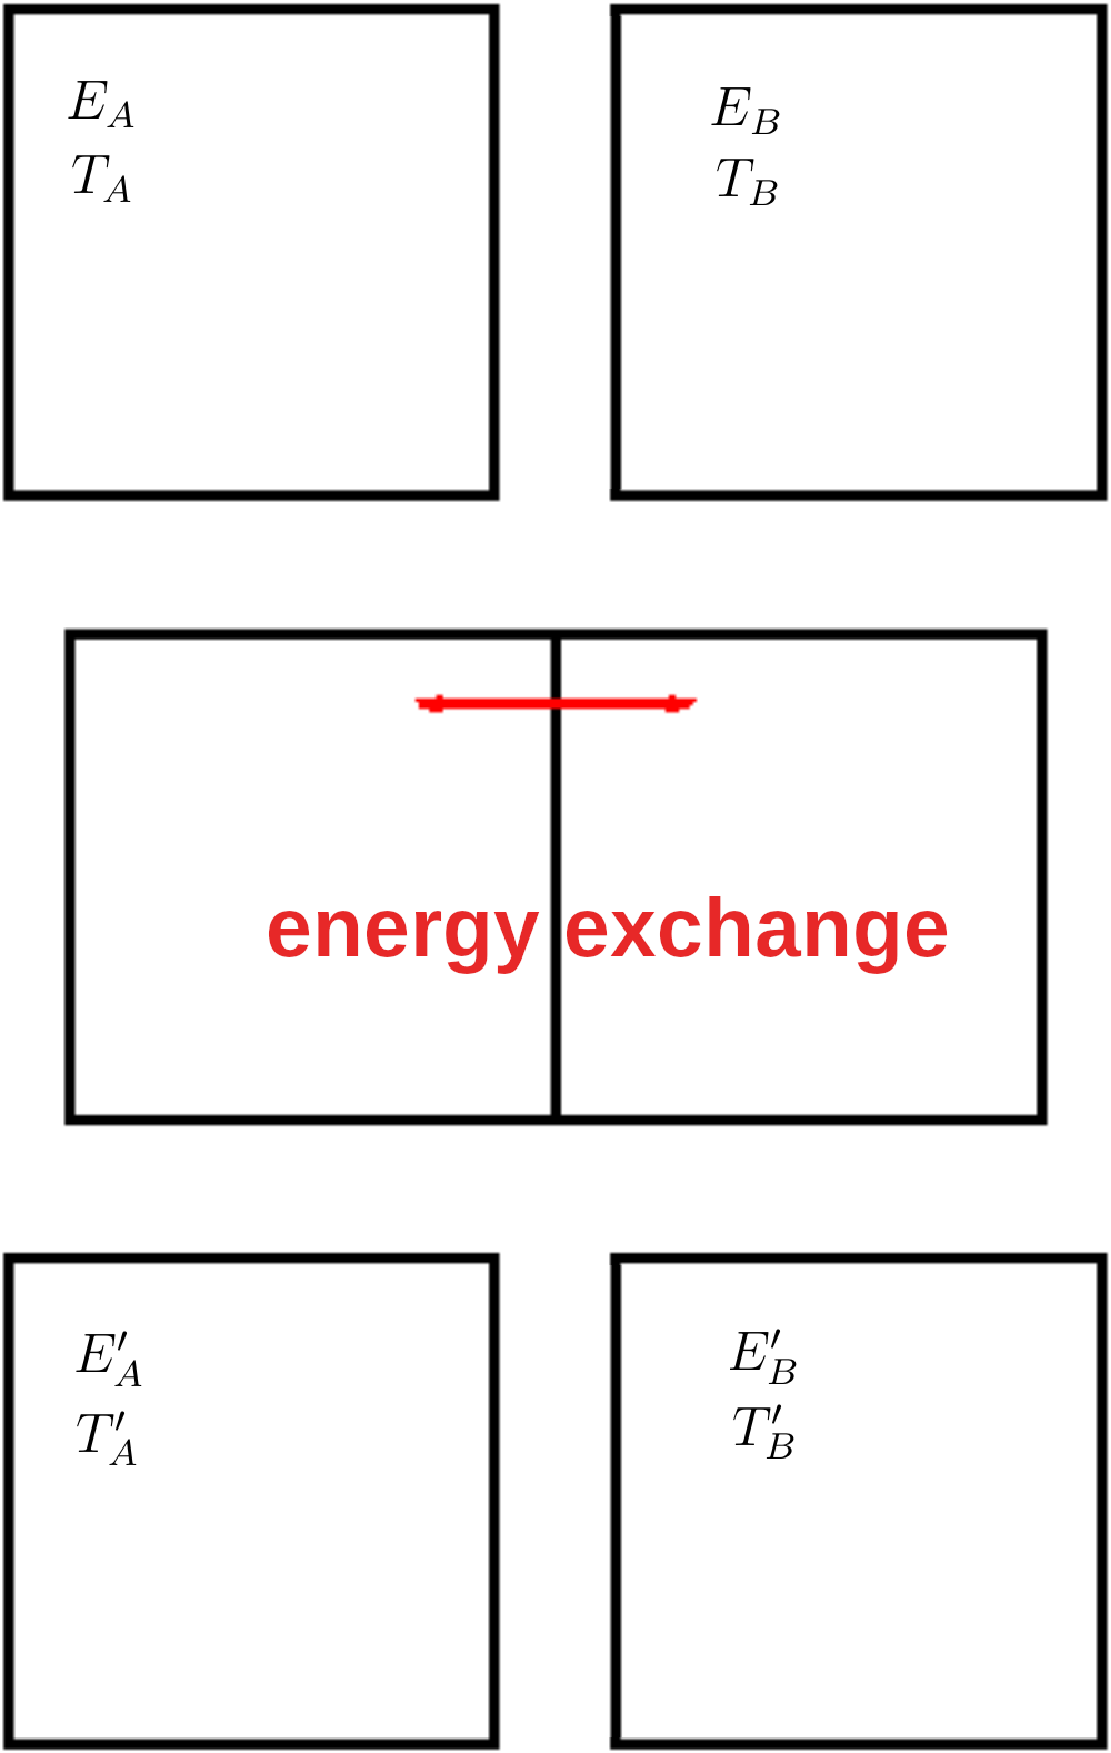
\includegraphics[width=0.5\textwidth]{figs/unit02_heat-exchange.pdf}
\end{center}

From everyday experience, we expect that this energy exchange will result in a net flow of energy from the hotter system to the colder system, cooling the former by heating the latter.
We will now check that the micro-canonical definition of temperature in \eq{eq:temperature} predicts this expected behaviour.
With $S \in \left\{A, B\right\}$, we can write
\begin{equation*}
  E_S' = E_S + \De E_S
\end{equation*}
and consider for simplicity the case where the change in energy is relatively small,
\begin{equation*}
  \left|\frac{\De E_S}{E_S}\right| \ll 1.
\end{equation*}
Since we can build up large changes in energy through a series of smaller changes, this assumption doesn't lead to any loss of generality.
We also know $\De E_B = -\De E_A$ thanks to conservation of energy.

Equation~\ref{eq:temperature} tells us that we need to consider the entropies as functions of $E_S$ and $E_S'$ in order to connect the temperatures to any flow of energy.
Because we don't change the number of particles in each system, we only need to consider the energy dependence of the entropy.
We assume $S(E)$ is continuous and infinitely differentiable,\footnote{This assumption breaks down at a \textit{phase transition}, where we would need to be more careful.  We will learn about phase transitions towards the end of the term.} which allows us to expand each of the final entropies $S(E_S')$ in a Taylor series,
\begin{equation*}
  S(E_S') = S(E_S + \De E_S) \approx S(E_S) + \left.\pderiv{S}{E}\right|_{E_S} \De E_S,
\end{equation*}
neglecting all $\cO\!\left(\De E_S^2\right)$ terms because we consider relatively small changes in energy.
What is the expression above in terms of the initial temperatures $T_S$?
\begin{mdframed}
  \ \\[50 pt]
\end{mdframed}

From the second law of thermodynamics, we know that the total entropy of these systems can never decrease as time passes:
\begin{equation}
  \label{eq:entropy_ineq}
  S(E_A) + S(E_B) \leq S(E_A + E_B) = S(E_A') + S(E_B').
\end{equation}
The final equality means that re-isolating the two subsystems doesn't change the entropy.
This is because $E_A'$ is not fixed and could take any value from zero to $E_A + E_B$ at the moment when the subsystems are re-isolated.
Computing the final entropy $S(E_A') + S(E_B')$ therefore requires summing over all possible values of $E_A'$, producing exactly the sum in \eq{eq:micro_sum} for the overall system.
We will see something similar when we consider the `Gibbs paradox' in Unit~4.

What do you find when you insert your linearized Taylor series into \eq{eq:entropy_ineq}?
\begin{mdframed}
  \ \\[100 pt]
\end{mdframed}
Applying conservation of energy should produce
\begin{equation*}
  \left(\frac{1}{T_A} - \frac{1}{T_B}\right) \De E_A \geq 0.
\end{equation*}
Recalling from \secref{sec:second_law} that equality holds only in extremely special cases, we can identify three possibilities consistent with this result.
If $T_A > T_B$, then $\left(\frac{1}{T_A} - \frac{1}{T_B}\right)$ is negative and we will generically have $\De E_A < 0$, so that energy flows out of the hotter system $\Om_A$ and into the colder one.
Our restriction to natural systems means this flow of energy reduces the higher temperature, and increases the lower temperature, bringing the temperatures of the two subsystems closer to each other.
Similarly, if $T_A < T_B$, we will generically have $\De E_A > 0$, meaning that energy still flows from the hotter system $\Om_B$ into the colder one, again reducing the difference in their temperatures.
We can finally conclude that $T_A = T_B$ is the very special case where there is no energy flow, $\De E_S = 0$, keeping the temperatures the same.
All of this is exactly what we would expect based on our everyday experience of temperature as an intensive quantity.
% ------------------------------------------------------------------


\newpage
% ------------------------------------------------------------------
\renewcommand{\thisunit}{MATH327 Unit 3}
\renewcommand{\moddate}{Last modified 16 Feb.~2025}
\setcounter{section}{3}
\setcounter{subsection}{0}
\phantomsection
\addcontentsline{toc}{section}{Unit 3: Canonical ensemble}
\section*{Unit 3: Canonical ensemble}
\subsection{\label{sec:reservoir}The thermal reservoir}
\subsubsection{\label{sec:replicas}Replicas and occupation numbers}
While it is reasonable to forbid particle exchange, for example by sealing gases inside airtight containers, it is not practical to prevent energy exchange as would be needed to fully isolate statistical systems.
Any thermal insulator is imperfect, and any observation of the system would require exchanging energy with the external observer. % E.g., we want to analyse a gas in a container without having to include ourselves as part of this ``system''....
In practice it is more convenient to work with physical systems that are characterized by their (intensive) temperatures rather than their (extensive) internal energies.

\begin{shaded}
  This leads us to define the \textbf{canonical ensemble} to be a statistical ensemble characterized by its fixed temperature $T$ and conserved particle number $N$, with the temperature held fixed through contact with a \textbf{thermal reservoir}.
\end{shaded}

The second part of this definition connects the fixed temperature to the fundamental fact of energy conservation (the first law of thermodynamics).
This is done by proposing that our system of interest \Om is in thermal contact with a much larger external system $\Om_{\text{res}}$ --- the thermal reservoir, sometimes called a ``heat bath''.
The overall combined system $\Om_{\text{tot}} = \Om_{\text{res}} \otimes \Om$ is governed by the micro-canonical ensemble, with conserved total energy $E_{\text{tot}} = E_{\text{res}} + E \approx E_{\text{res}}$, while the energy $E$ of \Om is allowed to fluctuate. % TODO: Could note that approximation is motivated by extensivity of energy...
The key qualitative idea is that, in thermodynamic equilibrium, \Om has a negligible effect on the overall system.
In particular, the temperature of that overall system --- and therefore the temperature of $\Om$, by intensivity --- is set by the reservoir and remains fixed even as $E$ fluctuates.
This effectively generalizes the setup we used to analyse heat exchange in the previous section, where we saw that thermal contact causes a net flow of energy from hotter systems to colder systems.
When these systems are `natural', this cools the hotter one by heating the colder one.

The mathematical implementation of this argument, as developed by Gibbs, proceeds by considering a well-motivated ansatz for the form of the thermal reservoir $\Om_{\text{res}}$.
\textcolor{green}{The goal}, which will be useful to keep in mind as we go through the lengthy analysis, is to show that the specific form of $\Om_{\text{res}}$ is ultimately irrelevant.
This will allow us to work directly with the system of interest, $\Om$, independent of the details of the thermal reservoir that fixes its temperature.

Without further ado, we take $\Om_{\text{tot}}$ to consist of many ($R \gg 1$) identical \textbf{replicas} of the system \Om that we're interested in.
All of these replicas are in thermal contact with each other, and in thermodynamic equilibrium.\footnote{The thermal contact between any two replicas can be indirect, mediated by a sequence of intermediate replicas.  This transitivity of thermodynamic equilibrium is sometimes called the \href{https://en.wikipedia.org/wiki/Zeroth_law_of_thermodynamics}{zeroth law of thermodynamics}.  It declares that if systems $\Om_A$ \& $\Om_B$ are in thermodynamic equilibrium while systems $\Om_B$ \& $\Om_C$ are in thermodynamic equilibrium, then $\Om_A$ \& $\Om_C$ must also be in thermodynamic equilibrium.}
Choosing any one of the replicas to be the system of interest, $\Om$, the other $R - 1 \approx R$ replicas collectively form the thermal reservoir $\Om_{\text{res}}$.
Assuming we want to study reasonable systems $\Om$, this ansatz ensures that $\Om_{\text{res}}$ is also reasonable, simply much larger.

An extremely small example of this setup is illustrated by the figures below, where the system of interest is just $N = 2$ spins.
For now we assume the spins are \textit{distinguishable}, so that $\downarrow\uparrow$ and $\uparrow\downarrow$ are both distinct micro-states.
This means that each individual replica has the $M = 4$ micro-states $\om_i$ defined below.
\begin{center}
  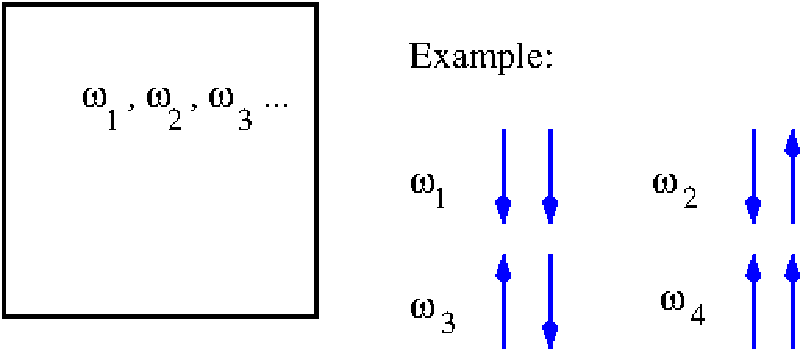
\includegraphics[width=0.7\textwidth]{figs/unit03_spin-system.pdf}
\end{center}
To form the overall system $\Om_{\text{tot}}$ we now bring together the $R = 9$ replicas shown below.
We draw boxes around each replica to remind us that they are allowed to exchange only energy with each other, while the $N = 2$ spins per replica are fixed in place.
We pick out one of these replicas (in the red box) to serve as the system \Om we will consider.
The other $8$ are the thermal reservoir $\Om_{\text{res}}$ that fixes the temperature of $\Om$.
\begin{center}
  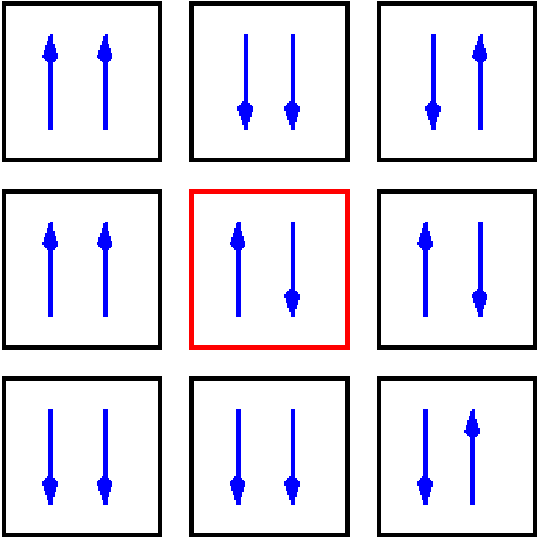
\includegraphics[width=0.7\textwidth]{figs/unit03_spin-reservoir.pdf}
\end{center}

A convenient way to analyse the overall system of $R$ replicas, $\Om_{\text{tot}}$, is to define the \textbf{occupation number} $n_i$ to be the number of replicas that adopt the micro-state $\om_i \in \Om$ in any given micro-state of $\Om_{\text{tot}}$.
The index $i \in \left\{1, 2, \cdots, M\right\}$ runs over all $M$ micro-states of $\Om$.
In the example above, three of the replicas have the micro-state $\om_1 = \downarrow\downarrow$, meaning $n_1 = 3$.
What are the occupation numbers $\left\{n_2, n_3, n_4\right\}$ for the other three $\om_i$ in the figures above?
Are all replicas are accounted for, $\sum_i n_i = R$?
\begin{mdframed}
  \ \\[50 pt]
\end{mdframed}
Normalizing the occupation number by $R$ gives us a well-defined \textit{occupation probability}, $p_i = n_i / R$ with $\sum_i p_i = 1$. % Notation anticipates that canonical probability for micro-state om_i will be p_i, since we would then expect R*p_i = n_i replicas to exhibit this micro-state...
At the moment, this $p_i$ is the probability that if we choose a replica at random it will be in micro-state $\om_i$.

Now let us consider conservation of energy, which continues to apply to the total energy $E_{\text{tot}}$ of the overall system $\Om_{\text{tot}}$.
We assume that each replica's energy $E_r$ is independent of all the other replicas.
This is guaranteed for the non-interacting systems we will focus on until Unit~9, and also holds when interactions are allowed within each replica but not between different replicas.
The thermal contact between replicas allows $E_r$ to fluctuate subject to conservation of $E_{\text{tot}}$, but there are at most $M$ possible values $E_i$ it can have, corresponding to the $M$ micro-states $\om_i \in \Om$.
Some distinct micro-states $\om_i \ne \om_j$ may have the same energy $E_i = E_j$, which doesn't affect the analysis.
This allows us to rearrange a sum over replicas into a sum over the micro-states of $\Om$:
\begin{equation}
  \label{eq:canon_Etot}
  E_{\text{tot}} = \sum_{r = 1}^R E_r = \sum_{i = 1}^M n_i E_i,
\end{equation}
with the occupation number $n_i$ counting how many times micro-state $\om_i$ appears among the $R$ replicas.
We can assume that $R$ and $M$ are both finite, so we don't need to worry about rearranging the sums.
% ------------------------------------------------------------------



% ------------------------------------------------------------------
\subsubsection{\label{sec:canon_part}Partition function}
Following Gibbs, we've taken the thermal reservoir $\Om_{\text{res}}$ to consist of $R - 1$ replicas of the system of interest, $\Om$.
The next step is to further simplify the mathematics by assuming that the overall $R$-replica system $\Om_{\text{tot}}$ is fully specified by a fixed set of $M$ occupation numbers $\left\{n_i\right\}$.
This is equivalent to assuming that the occupation probabilities $\left\{p_i\right\}$ are constant in time, as a reflection of thermodynamic equilibrium.
From \eq{eq:canon_Etot}, we see that this ensures conservation of the total energy $E_{\text{tot}}$, and we can apply the micro-canonical tools we developed in the previous unit.
Recall our ultimate \textcolor{green}{goal} of showing that such details of the thermal reservoir are irrelevant to the system $\Om$.

Based on the conservation of $E_{\text{tot}}$, we want to determine the (intensive) temperature of $\Om_{\text{tot}}$, which fixes the temperature of the system of interest, $\Om$.
According to our previous work, to do this we first need to compute the overall number of micro-states $M_{\text{tot}}$ as a function of $E_{\text{tot}}$, from which we can derive the micro-canonical entropy and temperature since the system is in thermodynamic equilibrium.
From the fixed occupation numbers $n_i$, we already know how many times each micro-state $\om_i$ appears among the $R$ replicas.
To determine $M_{\text{tot}}$ we just need to count how many possible ways there are of distributing the $\left\{n_i\right\}$ micro-states among the $R$ replicas.

If we consider first the micro-state $\om_1$, the number of possible ways of distributing $n_1$ copies of this micro-states among the $R$ replicas is just the binomial coefficient
\begin{equation*}
  \binom{R}{n_1} = \frac{R!}{n_1! \; (R - n_1)!}.
\end{equation*}
Moving on to $\om_2$, we need to keep in mind that $n_1$ replicas have already been assigned micro-state $\om_1$, so there are only $R - n_1$ replicas left to choose from.
What is the resulting number of possible ways of distributing these $n_2$ micro-states?
\begin{mdframed}
  \ \\[50 pt]
\end{mdframed}
Repeating this process for all micro-states $\left\{\om_1, \om_2, \cdots, \om_M\right\}$, recalling $\left(R - \sum_i n_i \right)! = 0! = 1$, you should obtain a product that `telescopes' to
\begin{equation}
  \label{eq:telescoped}
  M_{\text{tot}} = \frac{R!}{n_1! \; n_2! \; \cdots \; n_M!}.
\end{equation}
This confirms that the order in which we assign micro-states to replicas is irrelevant, since integer multiplication is commutative.

Thanks to thermodynamic equilibrium, the entropy of the micro-canonical $\Om_{\text{tot}}$ is
\begin{equation*}
  S(E_{\text{tot}}) = \log M_{\text{tot}} = \log(R!) - \sum_{i = 1}^M \log(n_i!),
\end{equation*}
where the dependence on $E_{\text{tot}}$ enters through the occupation numbers via \eq{eq:canon_Etot}.
With $R \gg 1$ and $n_i \gg 1$ for all $i = 1, \cdots, M$, we can approximate each of these logarithms using the first two terms in \href{https://en.wikipedia.org/wiki/Stirling's_approximation}{Stirling's formula},
\begin{align*}
  \log(N!) & = N \log N - N + \cO(\log N) \approx N \log N - N &
  \mbox{for } N & \gg 1.
\end{align*}
In order for \textit{every} occupation number to be large, $n_i \gg 1$, the number of replicas must be much larger than the number of micro-states of $\Om$.
As we have discussed before, the number of micro-states $M$ is typically a very large number, so with $R \gg M$ we are formally considering truly enormous thermal reservoirs!
This enormity helps ensure that the detailed form of the reservoir will be irrelevant.

\newpage % WARNING: FORMATTING BY HAND
Using the approximation above, what do you find for $S(E_{\text{tot}})$ in terms of $R$ and $n_i$?
What is the entropy in terms of the occupation probabilities $p_i = n_i / R$?
\begin{mdframed}
  $\displaystyle S(E_{\text{tot}}) = \log(R!) - \sum_{i = 1}^M \log(n_i!) \approx $ \\[100 pt]
\end{mdframed}
% This gives the result we would expect from extensivity.

In your result, the dependence on $E_{\text{tot}}$ now enters through the occupation probabilities $p_i$.
In order to determine the temperature, we have to express the entropy explicitly in terms of $E_{\text{tot}}$.
We do this by applying our knowledge that thermodynamic equilibrium implies maximal entropy.

Following the same steps as in \secref{sec:second_law}, we maximize the entropy, now with two Lagrange multipliers to account for two constraints on the occupation probabilities:
\begin{align*}
  \sum_{i = 1}^M p_i & = 1 &
  \sum_{i = 1}^M n_i E_i & = R \sum_{i = 1}^M p_i E_i = E_{\text{tot}}.
\end{align*}
Writing everything in terms of occupation probabilities, we therefore need to maximize the modified entropy
\begin{equation*}
  \Sbar = -R \sum_{i = 1}^M p_i \log p_i + \al\left(\sum_{i = 1}^M p_i - 1\right) - \be\left(R \sum_{i = 1}^M p_i E_i - E_{\text{tot}}\right).
\end{equation*}
Here we've chosen the sign of \be for later convenience.
What is the occupation probability $p_k$ that maximizes $\Sbar$?
\begin{mdframed}
  $\displaystyle 0 = \pderiv{\Sbar}{p_k} = $ \\[120 pt]
\end{mdframed}

\newpage % WARNING: FORMATTING BY HAND
By defining a new parameter $Z$ in terms of $\al$, you should find
\begin{equation}
  \label{eq:occ_prob}
  p_k = \frac{1}{Z} e^{-\be E_k}.
\end{equation}
As before, we need to fix the parameters $\left\{Z, \be\right\}$ by demanding that the two constraints above are satisfied.
The first of these constraints is straightforward and produces an important result:
\begin{equation}
  \label{eq:part_func}
  1 = \sum_{i = 1}^M p_i = \frac{1}{Z} \sum_{i = 1}^M e^{-\be E_i} \qquad \implies \qquad Z(\be) = \sum_{i = 1}^M e^{-\be E_i}.
\end{equation}

\begin{shaded}
  Eq.~\ref{eq:part_func} defines the canonical \textbf{partition function} $Z(\be)$, a fundamental quantity in the canonical ensemble, from which many other derived quantities can be obtained.
\end{shaded}

$Z(\be)$ still depends on the other as-yet-unknown parameter $\be(E_{\text{tot}})$.
By applying our second constraint, \eq{eq:canon_Etot}, we can relate \be to $E_{\text{tot}}$:
\begin{equation}
  \label{eq:canon_aveE}
  E_{\text{tot}} = R \sum_{i = 1}^M p_i E_i = \frac{R}{Z(\be)} \sum_{i = 1}^M E_i \; e^{-\be E_i} = R \frac{\sum_{i = 1}^M E_i \; e^{-\be E_i}}{\sum_{j = 1}^M e^{-\be E_j}}.
\end{equation}
This relation is a bit complicated, but will suffice for our goal of expressing the entropy in terms of $E_{\text{tot}}$.
Inserting \eq{eq:occ_prob} for $p_i$ into your earlier result for the entropy, what do you obtain upon applying Eqs.~\ref{eq:part_func} and \ref{eq:canon_aveE}?
\begin{mdframed}
  $\displaystyle S(E_{\text{tot}}) = -R \sum_{i = 1}^M p_i \log p_i = $ \\[100 pt]
\end{mdframed}
There is a pleasant simplification when we take the derivative to determine the temperature.
Defining $\be' \equiv \pderiv{}{E_{\text{tot}}} \be(E_{\text{tot}})$, we have
\begin{equation*}
  \frac{1}{T} = \pderiv{}{E_{\text{tot}}} S(E_{\text{tot}}) = \pderiv{}{E_{\text{tot}}} \left[E_{\text{tot}} \be + R\log Z(\be)\right] = \be + E_{\text{tot}} \be' + R \frac{1}{Z} \pderiv{Z(\be)}{\be} \be' .
\end{equation*}
Using \eq{eq:canon_aveE} we can compute
\begin{equation*}
  \frac{1}{Z} \pderiv{Z(\be)}{\be} = \frac{1}{Z} \pderiv{}{\be} \sum_{i = 1}^M e^{-\be E_i} = -\frac{1}{Z} \sum_{i = 1}^M E_i \; e^{-\be E_i} = -\sum_{i = 1}^M p_i E_i = -\frac{E_{\text{tot}}}{R},
\end{equation*}
so that we don't need to figure out the explicit form of $\be'$:
\begin{equation}
  \label{eq:beta}
  \frac{1}{T} = \be + E_{\text{tot}} \be' - E_{\text{tot}} \be' = \be .
\end{equation}

What's truly remarkable about Eqs.~\ref{eq:occ_prob}, \ref{eq:part_func} and \ref{eq:beta} is that they make no reference to the $R$ replicas or any extensive quantity of the overall system, such as $E_{\text{tot}}$ --- all information about the thermal reservoir has vanished.
This is \textcolor{green}{the goal} we have been pursuing since the start of this unit!
The large thermal reservoir is still present to fix the temperature $T$ characterizing the canonical system $\Om$, but beyond that nothing about it is relevant (or even knowable) in the canonical approach.
Every aspect of \Om can now be specified in terms of its fixed temperature $T$ and conserved particle number $N$, starting with the parameter $\be = 1 / T$.

In particular, the partition function from \eq{eq:part_func} is simply
\begin{equation}
  \label{eq:canon_part_func}
  Z(T) = \sum_{i = 1}^M e^{-E_i / T}.
\end{equation}
and together with \be specifies the probabilities
\begin{equation}
  \label{eq:canon_prob}
  p_i = \frac{1}{Z} e^{-E_i / T}
\end{equation}
from \eq{eq:occ_prob}.
This $p_i$ is now the thermodynamic equilibrium probability that \Om adopts micro-state $\om_i$ with (non-conserved) internal energy $E_i$.
This probability distribution is called either the \textbf{Boltzmann distribution} or the \textbf{Gibbs distribution}, while $e^{-E_i / T}$ itself is known as a \textbf{Boltzmann factor}.
All micro-states with the same energy have the same probability in thermodynamic equilibrium, which is consistent with the micro-canonical behaviour we saw in Unit~2.
% ------------------------------------------------------------------



% ------------------------------------------------------------------
\subsection{\label{sec:canon_derived}Internal energy, heat capacity, and entropy}
In addition to fixing the temperature of the system $\Om$, the thermal reservoir also allows the internal energy of \Om to fluctuate.
The system simply exchanges energy with the reservoir, satisfying the first law of thermodynamics.
Although the internal energy fluctuates, its expectation value $\vev{E}$ is an important derived quantity in thermodynamic equilibrium.
Applying the general definition from \eq{eq:expect_disc} to the probability space of the canonical ensemble,
\begin{equation*}
  \vev{E}\!(T) = \sum_{i = 1}^M E_i \; p_i = \frac{1}{Z} \sum_{i = 1}^M E_i \; e^{-\be E_i}.
\end{equation*}
Here we highlight the dependence of $\vev{E}$ on the temperature, and also freely interchange $\be = 1 / T$.

\newpage % WARNING: FORMATTING BY HAND
The expression above may look familiar from our work in the previous section:
\begin{mdframed}
  $\displaystyle \pderiv{}{\be} \log Z = $ \\[100 pt]
\end{mdframed}
In this case it is easier to take the derivative with respect to \be as opposed to
\begin{equation}
  \label{eq:beta_T}
  \pderiv{}{\be} = \pderiv{T}{\be} \pderiv{}{T} = -\frac{1}{\be^2} \pderiv{}{T} = -T^2 \pderiv{}{T}.
\end{equation}

In \secref{sec:temp}, we saw that `natural' micro-canonical systems exhibit higher (derived) temperatures for larger (conserved) internal energies.
Here, in the canonical approach, the average internal energy $\vev{E}$ is the derived quantity while the temperature is fixed.
From our everyday experience, we expect a similar direct relation between temperature and energy, which the following result confirms.

\begin{shaded}
  The \textbf{heat capacity} is defined to be
  \begin{equation}
    \label{eq:heat_cap}
    c_v = \pderiv{}{T} \vev{E},
  \end{equation}
  and is always non-negative, $c_v \geq 0$.
\end{shaded}

The subscript indicates that the volume of the system is kept fixed; we'll consider the role of the volume more carefully starting in Unit~4.
In a homework assignment you will confirm $c_v \geq 0$ by deriving a \textbf{fluctuation--dissipation} (or \textbf{fluctuation--response}) \textbf{relation}.
That relation will be a special case of a \href{https://en.wikipedia.org/wiki/Fluctuation-dissipation_theorem}{more general theorem}, and will connect the fluctuations of the internal energy around its expectation value, $\left(E_i - \vev{E}\right)^2$, to the energy's \textit{response} to a change in temperature, $\pderiv{}{T} \vev{E}$.
Only extremely special cases will produce $c_v = 0$, meaning that the heat capacity is generically positive, in agreement with our intuition that higher temperatures produce larger internal energies.

\newpage % WARNING: FORMATTING BY HAND
Finally, we can compute the entropy of \Om with no reference to the thermal reservoir, apart from its role fixing the temperature in thermodynamic equilibrium.
Since the general definition of the entropy in \eq{eq:entropy} continues to hold for the canonical ensemble, we just need to insert the probabilities $p_i$ from \eq{eq:canon_prob}:
\begin{mdframed}
  $\displaystyle S(T) = -\sum_{i = 1}^M p_i \log p_i = $ \\[100 pt]
\end{mdframed}
You should find that the entropy depends on $\log Z$.
% ------------------------------------------------------------------



% ------------------------------------------------------------------
\subsection{\label{sec:Helmholtz}Helmholtz free energy}
This dependence of the entropy on $\log Z$ is in accordance with our earlier claim that the partition function is a fundamental quantity in the canonical ensemble.
Recalling from \eq{eq:canon_part_func} that $Z$ is a sum over all micro-states, we can view this result as the canonical counterpart to the micro-canonical entropy being the logarithm of the number of micro-states.
(Thermodynamic equilibrium is required in both cases.)
This motivates the following definition of a quantity with the dimensions of energy that is related to $\log Z$, which provides simpler and more elegant expressions for the derived quantities we considered above.

\begin{shaded}
  The \textbf{Helmholtz free energy} of a system in the canonical ensemble is
  \begin{align}
    \label{eq:helmholtz}
    F(T) & = -T \log Z(T) &
    F(\be) & = -\frac{\log Z(\be)}{\be},
  \end{align}
  where $Z$ is the partition function of the system.
  In terms of this free energy, Eqs.~\ref{eq:canon_part_func} and \ref{eq:canon_prob} are
  \begin{align*}
    Z & = e^{-F / T} &
    p_i & = e^{(F - E_i) / T}.
  \end{align*}
\end{shaded}

\newpage % WARNING: FORMATTING BY HAND
The Helmholtz free energy is named after \href{https://en.wikipedia.org/wiki/Hermann_von_Helmholtz}{Hermann von Helmholtz} and reveals its usefulness when we take its derivative.
The derivative involves $\pderiv{}{T} \log Z$, which is worth collecting in advance based on \eq{eq:beta_T}:
\begin{mdframed}
  $\displaystyle -\pderiv{}{T}\left(\frac{F(T)}{T}\right) = \pderiv{}{T} \log Z(T) = $ \\[50 pt]
  $\displaystyle \pderiv{}{T} F(T) = $ \\[50 pt]
\end{mdframed}
From these results we can read off the more elegant expressions promised above:
\begin{align}
  S(T) & = -\pderiv{}{T} F(T) \label{eq:canon_entropy-F} \\
  \vev{E}\!(T) & = -T^2 \pderiv{}{T}\left(\frac{F(T)}{T}\right) = \pderiv{}{\be}\left[\be F(\be)\right] = T S(T) + F(T). \label{eq:canon_energy-F}
\end{align}
% ------------------------------------------------------------------



% ------------------------------------------------------------------
\subsection{\label{sec:spin_info}The physics of information}
As a first application of the canonical ensemble, we will explore physically observable effects that depend on the information content of a statistical system.
A famous scientific question illustrating the importance of information, which you may have heard of, is the \href{https://en.wikipedia.org/wiki/Black_hole_information_paradox}{black hole information paradox}.
However, that topic is well beyond the scope of this module since it depends on quantum mechanics and general relativity in addition to statistical mechanics.
Here we will consider simple spin systems as introduced in \secref{sec:ensemble}, contrasting the behaviour of their average internal energy $\vev{E}$ and entropy $S$ depending on whether or not the spins can (in principle) be distinguished from each other.
It's important to appreciate that the ``information'' discussed here is an intrinsic property of the system --- what is \textit{knowable} about it in principle.
It does not matter whether or not any observer actually knows this information; so long as it can possibly be known it will have an effect.

\subsubsection{\label{sec:spin_chain}Distinguishable spins in a solid}
We begin with the setup from \secref{sec:ensemble}: A system of $N$ spins arranged in a line, placed in an external magnetic field of strength $H$, and in thermodynamic equilibrium.
We further specify that the spins are embedded in a solid material that fixes their positions and prevents them from moving.
This allows them to be distinguished from one another: An observer can target an appropriate position in the solid to measure the corresponding spin.
Each spin measured in this way will be either parallel or anti-parallel to the magnetic field.
The canonical system therefore has $M = 2^N$ distinct micro-states $\om_i$ with energies $E_i$ and probabilities $p_i = \frac{1}{Z} e^{-E_i / T}$, each defined by the orientations of all $N$ spins.

To streamline our notation, we can represent the orientation of the $n$th spin as $s_n \in \left\{1, -1\right\}$, where $s_n = 1$ indicates alignment parallel to the field and $s_n = -1$ indicates alignment anti-parallel to the field.
With this notation, the internal energy of the system in micro-state $\om_i$ specified by the $N$ spins $\left\{s\right\}$ is simply
\begin{equation}
  \label{eq:spin_energy}
  E_i = -H \sum_{n = 1}^N s_n.
\end{equation}
To compute the canonical partition function $Z_D$, where the subscript reminds us of the spins' distinguishability, we have to sum over all $2^N$ possible spin configurations $\left\{s\right\}$.
In this process we can save some space by defining the dimensionless variable $x = \be H = \frac{H}{T}$:
\begin{align}
  Z_D & = \sum_{s_1 = \pm 1} \cdots \sum_{s_N = \pm 1} e^{-\be E_i} = \sum_{s_1 = \pm 1} \cdots \sum_{s_N = \pm 1} \exp\left[x \sum_{n = 1}^N s_n\right] \cr
      & = \sum_{s_1 = \pm 1} \cdots \sum_{s_N = \pm 1} e^{x s_1} \cdots e^{x s_N} = \left(\sum_{s_1 = \pm 1} e^{x s_1}\right) \cdots \left(\sum_{s_N = \pm 1} e^{x s_N}\right) \cr
      & = \left(\sum_{s = \pm 1} e^{x s}\right)^N = \left(e^x + e^{-x}\right)^N = \left[2\cosh\left(\be H\right)\right]^N, \label{eq:spin_part_func}
\end{align}
distributing the summations since all the spins are independent of each other.

The corresponding Helmholtz free energy
\begin{equation}
  \label{eq:dist_Helm}
  F_D(\be) = -\frac{\log Z(\be)}{\be} = -\frac{N \log\left[2\cosh\left(\be H\right)\right]}{\be}
\end{equation}
is all we need to compute the average internal energy:
\begin{mdframed}
  $\displaystyle \vev{E}_D = \pderiv{}{\be}\left[\be F_D(\be)\right] = $ \\[90 pt]
\end{mdframed}
From this we immediately obtain the entropy
\begin{equation}
  \label{eq:dist_entropy}
  S_D = \be\left(\vev{E}_D - F_D\right) = -N\be H \tanh\left(\be H\right) + N \log\left[2\cosh\left(\be H\right)\right].
\end{equation}
These results for $\vev{E}_D$ and $S_D$ are plotted on the next page as functions of $\frac{T}{H} = \frac{1}{\be H}$, using \href{https://github.com/daschaich/MATH327_2025/blob/main/lecture_notes/unit03_distinguish.py}{this Python code}.
Since both these quantities are extensive, we normalize them by showing $\frac{\vev{E}_D}{NH}$ and $\frac{S_D}{N}$.

\begin{center}
  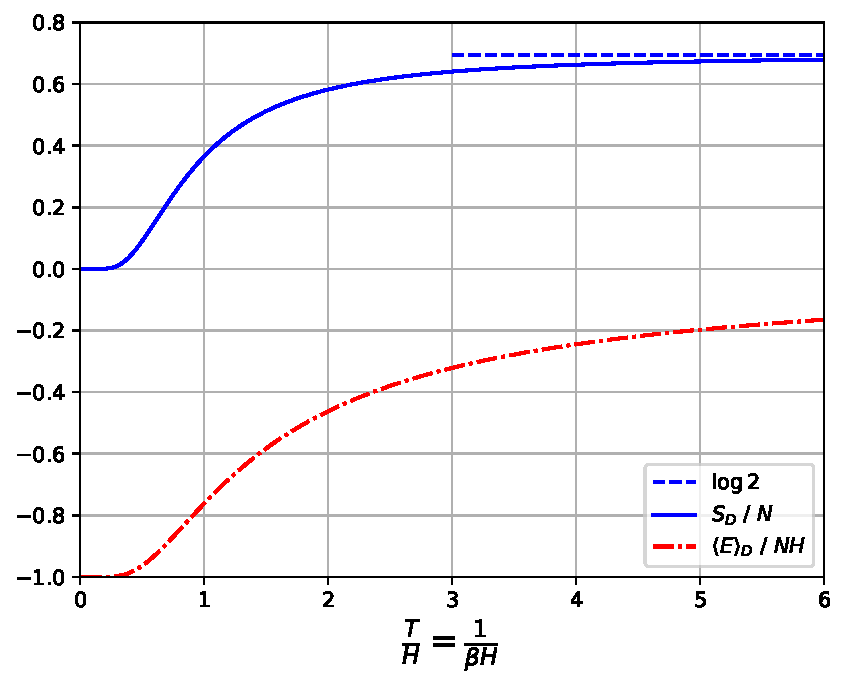
\includegraphics[width=0.9\textwidth]{figs/unit03_distinguish.pdf}
\end{center}

Let's analyse the asymptotic behaviour of these functions, starting with \textbf{low temperatures}.
In contrast to the micro-canonical \eq{eq:spin_temp}, in the canonical ensemble there is no issue with taking the independent variable $T \to 0$.
This corresponds to $\be H \to \infty$ and $\tanh\left(\be H\right) \to 1$, approaching the ``ground-state'' energy $E_{\text{min}} = E_0 = -NH$ you computed in \secref{sec:temp}.
This energy is only produced by the single micro-state in which all the spins are aligned with the magnetic field, $s_n = 1$ for all $n$ (or $n_+ = N$ and $n_- = 0$ in the notation from \secref{sec:temp}).
Correspondingly, $\log\left[2\cosh\left(\be H\right)\right] \to \log e^{\be H} = \be H$ and the two terms in \eq{eq:dist_entropy} cancel out, so that $S_D \to 0$.
This vanishing entropy is a generic consequence of temperatures approaching \textit{absolute zero}.

For low but non-zero temperatures, $\vev{E}_D$ and $S_D$ will be affected by the non-zero probability for the system to adopt micro-states $\om_i$ with higher energies $E_i > E_0$.
These higher-energy configurations are often referred to as ``excited states''.
Note that each energy $E_i > E_0$ may correspond to many different micro-states.
For example, in \secref{sec:temp} you also computed the energy $E_1 = -(N - 2)H$ of the first excited state, which is realized by the $N$ distinct micro-states with $n_- = 1$.
In the case of spin systems, we can instead refer to \textit{energy levels} that are all separated by a constant \textit{energy gap} $\De E \equiv E_{n_- + 1} - E_{n_-} = 2H$.

\newpage % WARNING: FORMATTING BY HAND
We can compute the effects of the higher energy levels at low temperatures $\be H \gg 1$ by expanding $\vev{E}_D$ in powers of $e^{-\be H} \ll 1$.
What is the first temperature-dependent term in this expansion?
\begin{mdframed}
  $\displaystyle \frac{\vev{E}_D}{NH} = $ \\[100 pt]
\end{mdframed}
You should find that the excited-state effects are \textit{exponentially} suppressed by the energy gap $\De E$ at low temperatures,
\begin{equation*}
  \frac{\vev{E}_D}{NH} = -1 + 2e^{-\be \De E} + \cO\left(e^{-2\be \De E}\right).
\end{equation*}
This is a generic feature of canonical systems with a non-zero energy gap, and is due to the exponentially suppressed probability for the system to adopt any of the micro-states with the higher energy,
\begin{equation*}
  \frac{\frac{1}{Z} e^{-\be E_{n_- + 1}}}{\frac{1}{Z} e^{-\be E_{n_-}}} = e^{-\be \De E}.
\end{equation*}

The low-temperature expansion of \eq{eq:dist_entropy} for the entropy in powers of $e^{-\be H} \ll 1$ is similar:
\begin{mdframed}
  $\displaystyle \frac{S_D}{N} = $ \\[100 pt]
\end{mdframed}
Here the leading term includes a linear factor of $\be \De E \gg 1$, but this can't overcome the now-expected exponential suppression:
\begin{equation*}
  \frac{S_D}{N} = \be \De E e^{-\be \De E} + e^{-\be \De E} + \cO\left(\be \De E e^{-2\be \De E}\right).
\end{equation*}

In the limit of \textbf{high temperatures} we should instead expand in powers of the small factor $\be H \ll 1$.
This is straightforward for $\vev{E}_D$:
\begin{equation*}
  \frac{\vev{E}_D}{NH} = -\tanh\left(\be H\right) = -\be H + \frac{\left(\be H\right)^3}{3} + \cO\left(\left[\be H\right]^5\right),
\end{equation*}
which vanishes $\sim$$\frac{1}{T}$ as $T \to \infty$.
This matches the micro-canonical behaviour we saw for this system from \eq{eq:spin_temp}, where the derived temperature diverged as the conserved energy approached zero.

For the entropy, there is a similar connection to micro-canonical behaviour at high temperatures:
\begin{mdframed}
  $\displaystyle \frac{S_D}{N} = $ \\[100 pt]
\end{mdframed}
As $\frac{T}{H} \to \infty$, the result
\begin{equation*}
  \frac{S_D}{N} = \log 2 - \frac{\left(\be H\right)^2}{2} + \cO\left(\left[\be H\right]^4\right)
\end{equation*}
approaches the asymptotic value $S_D \to N\log 2 = \log M$ for the $M = 2^N$ micro-states (with different energies).
Conceptually, in this limit the energy of each spin is negligible compared to the temperature, and the system approximately behaves as though the energy were zero for all micro-states (and hence conserved).
% ------------------------------------------------------------------



% ------------------------------------------------------------------
\subsubsection{Indistinguishable spins in a gas}
Next, let's consider nearly the same setup, with $N$ spins in thermodynamic equilibrium, in an external magnetic field of strength $H$.
The only difference is that now the spins are allowed to move, like particles in a one-dimensional gas.
We demand that they move slowly, so that we can ignore their kinetic energy and the total energy of the system continues to be given by \eq{eq:spin_energy}.
Since the spins don't interact with each other, they can freely move past each other, and even occupy the same space, making it impossible for them to be distinguished from one another. % Could remind that our starting point was noting we can't follow the motion of all the degrees of freedom...

To compute the fundamental canonical partition function (\eq{eq:canon_part_func}), we have to sum over the micro-states of the system.
These micro-states are no longer in one-to-one correspondence with the full configurations $\left\{s\right\}$ of the $N$ spins.
Because the spins are now indistinguishable, certain spin configurations also cannot be distinguished from each other.
The simplest example comes from the two-spin system considered in \secref{sec:replicas}, where the configurations $\downarrow\uparrow$ and $\uparrow\downarrow$ now both correspond to a single micro-state.
In this micro-state, we know only that one spin is $s_i = 1$ while the other is $s_k = -1$; it's not possible to distinguish which is which.

Generalizing, we can conclude that a single distinct micro-state corresponds to all possible permutations of spins with fixed $\left\{n_+, n_-\right\}$.
This means that each micro-state is now in one-to-one correspondence with the energy $E = -H(n_+ - n_-)$, which we can continue to organize as energy levels separated by a constant energy gap $\De E = 2H$.
As a quick example, enumerate the energy levels when $N = 4$ and list the spin configurations associated with the corresponding micro-states.
How many micro-states are there for $N$ spins?
\begin{mdframed}
  \ \\[120 pt]
\end{mdframed}

A convenient way to label these micro-states and energy levels is to define
\begin{equation*}
  E_k = -NH + 2Hk = -H(N - 2k)
\end{equation*}
for micro-state $\om_k$ with $k = n_- = 0, \cdots N$.
To compute the partition function $Z_I$, with the subscript reminding us about the spins' indistinguishability, we now have
\begin{equation}
  Z_I = \sum_{k = 0}^N e^{-\be E_k} = \sum_{k = 0}^N e^{\be H (N - 2k)} = e^{N\be H} \sum_{k = 0}^N \left(e^{-2\be H}\right)^k = e^{N\be H} \frac{1 - e^{-2(N + 1) \be H}}{1 - e^{-2\be H}}.
\end{equation}
The geometric series in the last step can be reconstructed by considering
\begin{equation*}
  \sum_{k = 0}^N x^k = \sum_{k = 0}^{\infty} x^k - \sum_{k = N + 1}^{\infty} x^k = \frac{1}{1 - x} - x^{N + 1} \sum_{\ell = 0}^{\infty} x^{\ell} = \frac{1}{1 - x} - \frac{x^{N + 1}}{1 - x}.
\end{equation*}

The corresponding Helmholtz free energy is
\begin{equation}
  \label{eq:indist_Helm}
  F_I(\be) = -\frac{\log Z_I(\be)}{\be} = -NH - \frac{\log\left[1 - e^{-2(N + 1) \be H}\right]}{\be} + \frac{\log\left[1 - e^{-2 \be H}\right]}{\be}.
\end{equation}
In contrast to \eq{eq:dist_Helm}, $F_I(\be)$ is no longer proportional to $N$.
In a homework assignment you will use $F_I$ to determine the average internal energy $\vev{E}_I$ and entropy $S_I$ shown in the figures on the next page, and also analyse the low- and high-temperature expansions like we did for the distinguishable case above.
Unlike our results for the distinguishable case, you will find that $\frac{\vev{E}_I}{NH}$ and $\frac{S_I}{N}$ depend on $N$, which requires us to fix $N = 4$ in the plots on the next page.
\begin{center} % Don't need centering, but this will provide consistent vertical spacing
  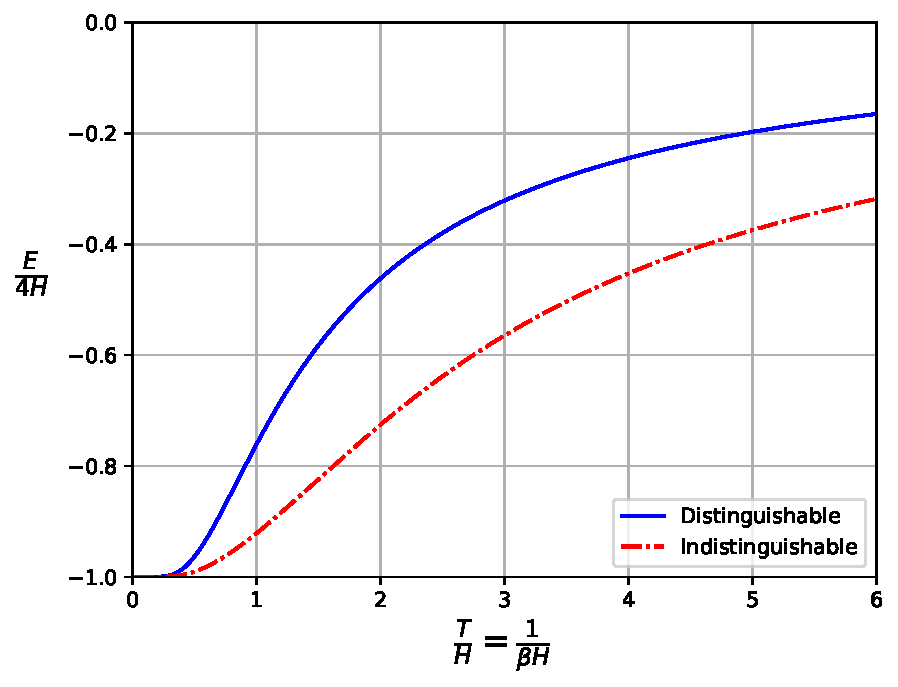
\includegraphics[width=0.475\textwidth]{figs/unit03_energies.pdf}\hfill 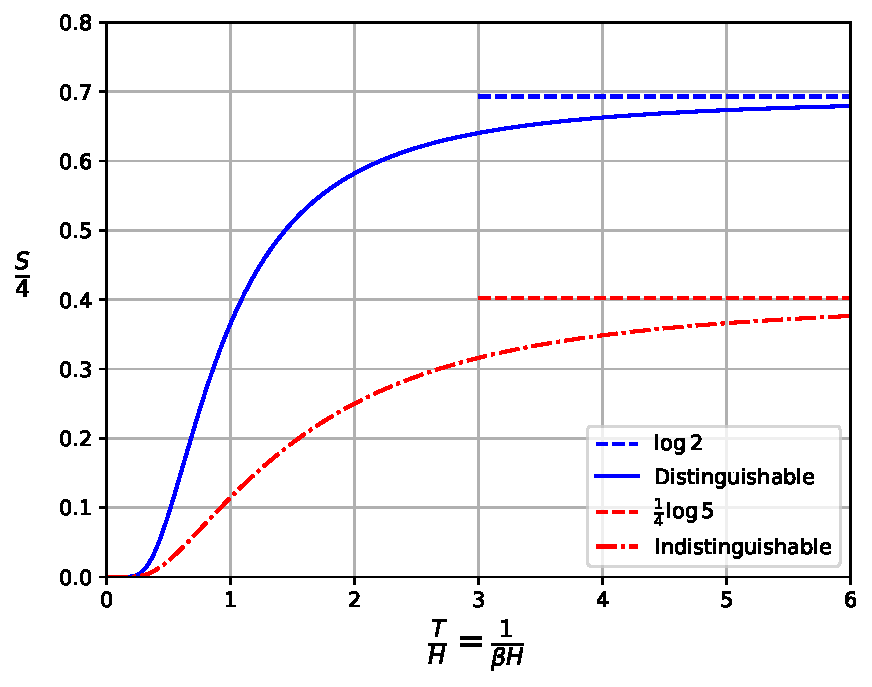
\includegraphics[width=0.475\textwidth]{figs/unit03_entropies.pdf}
\end{center}

The solid blue lines in these figures are exactly the distinguishable-spin results we previously discussed.
The red dash-dotted lines are the new results for indistinguishable spins.
We see that the same $T \to 0$ limits are approached in both cases: $E \to -NH$ and $S \to 0$.
At low temperatures, the indistinguishable results approach these limits more quickly --- they still feature exponential suppression of excited-state effects by the energy gap, $\propto$$e^{-\be \De E}$, but this now comes with additional factors of $N$.

At high temperatures there is an even more striking difference.
While the average internal energy $\vev{E}_I$ continues to vanish $\sim$$\frac{1}{T}$ as $T \to \infty$ (with different $N$ dependence), the entropy approaches the asymptotic value $S_I \to \log\left(N + 1\right) = \log M$ for the $M = N + 1$ micro-states.
This logarithmic dependence on $N$ is very different from the $S_D \to N\log 2$ limit we found for distinguishable spins, and reflects the exponentially smaller number of micro-states that exist for indistinguishable spins, $N + 1$ vs.\ $2^N$.

Finally, away from those low- and high-temperature limits, the left figure above shows a significant difference in the internal energies of the spin systems, depending only on whether or not the spins can be distinguished from each other in principle.
This is a physically measurable effect caused by the intrinsic information content of a statistical system, and a simple illustration of phenomena that remain at the leading edge of ongoing research.
As \href{https://en.wikipedia.org/wiki/Rolf_Landauer}{Rolf Landauer} put it in a famous 1991 essay: \href{https://scottaaronson.blog/?p=3327}{Information is physical}.
% ------------------------------------------------------------------


\newpage
% ------------------------------------------------------------------
\renewcommand{\thisunit}{MATH327 Unit 4}
\renewcommand{\moddate}{Last modified 23 Feb.~2025}
\setcounter{section}{4}
\setcounter{subsection}{0}
\phantomsection
\addcontentsline{toc}{section}{Unit 4: Ideal gases}
\section*{Unit 4: Ideal gases}
\subsection{\label{sec:regulate}Volume, energy levels, and partition function}
We now apply the canonical ensemble to investigate non-relativistic, classical, ideal gases.
Using statistical mechanics we will explore how the large-scale behaviours of such gases emerge from the properties of the particles that compose them.
The key particle properties are specified by the adjectives used above: \\[-24 pt]
\begin{itemize}
  \item \textbf{Classical} systems are those for which we can ignore the effects of quantum mechanics.
        Among other things, this allows us to simultaneously define both the position $(x, y, z)$ and the momentum $\vec p = (p_x, p_y, p_z)$ of each particle with arbitrary precision. % TODO: The `other things' include the possibility of labeling identical particles to distinguish them, which may be too much info to include here...
  \item \textbf{Non-relativistic} particles move with speeds small compared to the speed of light, which allows us to ignore small effects due to special relativity.
        The particles are therefore governed by the laws Isaac Newton published all the way back in 1687.
        In particular, the energy of each particle of mass $m$ is
        \begin{equation*}
          E_n = \frac{1}{2m} p_n^2,
        \end{equation*}
        where $p_n^2 = \vec p_n \cdot \vec p_n = (p_x)_n^2 + (p_y)_n^2 + (p_z)_n^2$ is the inner (or `dot') product of the momentum vector for the $n$th particle in the micro-state of interest.
  \item \textbf{Ideal} gases are those whose constituent particles don't interact with each other.
        As a result, the total energy of the gas is simply the sum of the energies of the $N$ individual particles,
        \begin{equation}
          \label{eq:momentum}
          E = \frac{1}{2m} \sum_{n = 1}^N p_n^2.
        \end{equation}
\end{itemize}

As is now familiar for the canonical ensemble, we consider the gas to be in thermodynamic equilibrium, and in thermal contact with a large external thermal reservoir with which it can exchange energy but not particles.
To prevent particle exchange, we can specify that the gas is enclosed in a cubic box with volume $V = L^3$.
The thermal reservoir fixes the temperature $T$ of the gas.

The starting point for our analysis is to compute the partition function
\begin{equation*}
  Z = \sum_i e^{-E_i / T}.
\end{equation*}
Unfortunately there is a challenge confronting this sum over all possible micro-states $\om_i$ of the $N$-particle system.
These micro-states depend on the momenta $\vec{p}_n$ for all $N$ particles, and it's intuitive to suppose that each component of $(p_x, p_y, p_z)_n$ is a continuously varying real number that can (in principle) be distinguished with arbitrary precision.
This implies an uncountably infinite set of distinct momenta and hence an uncountably infinite set of micro-states, making the summation above ill-defined.

To proceed, we \textit{regularize} the system so that there are a countable number of micro-states we can sum over to define the partition function.
We do this by positing that the particles' momentum components can take only discrete (or `quantized') values that depend on the volume of the box.
Specifically, we declare that the possible momenta are
\begin{align}
  \label{eq:quant_mom}
  \vec p & = (p_x, p_y, p_z) = \hbar \frac{\pi}{L} (k_x, k_y, k_z) &
  k_{x, y, z} & \in \Zbb.
\end{align}
The constant factor $\hbar$ (``h-bar'') is known as the (reduced) Planck constant, named after \href{https://en.wikipedia.org/wiki/Max_Planck}{Max Planck}).
Like the Boltzmann constant $k$, the Planck constant is another unit conversion factor (relating inverse length $\frac{1}{L}$ and momentum $p$), which is just $\hbar = 1$ in natural units.
Despite this, we will retain explicit factors of $\hbar$ in these lecture notes.

What are the energies that correspond to these discretized momenta?
\begin{mdframed}
  \ \\[60 pt] % WARNING: ADJUSTED SIZE BY HAND TO FILL REMAINDER OF PAGE
\end{mdframed}
You should find energies that fall into discrete \textit{energy levels}, somewhat similar to the spin system considered in \secref{sec:spin_info}.
Unlike the spin system, in this case the energy gaps between subsequent energy levels are not constant.

Similar discrete energy levels turn out to be realized in nature, thanks to quantum mechanics --- if you have previously studied quantum physics, you may spot a resemblance with a \href{https://en.wikipedia.org/wiki/Particle_in_a_box}{particle in a box}.
For the purposes of this module we can just adopt \eq{eq:quant_mom} as an ansatz. % TODO: Planck also introduced this ansatz as a desperate measure; a difference with bona fide quantum mechanics is the presence of a zero mode...
Even with this perspective, it will be useful to maximize the similarity with quantum physics.
We can do this by observing that negating any component of the momentum has no effect on the energy $E \propto p^2 \propto k^2$, and hence all non-zero $\pm k_i$ pairs make equal contributions to the partition function.
Therefore, restricting the discrete momenta to non-negative $k_{x, y, z} = 0, 1, 2, \cdots$ only changes $Z$ by a constant factor $C$, which cancels out in the expectation value of any observable that depends only on the inner product $p^2$:
\begin{equation*}
  \vev{f(p^2)} = \frac{\sum_{k_{x, y, z} \in \Zbb} f(p^2) e^{-E_i / T}}{Z} \quad \lra \quad \frac{C\sum_{k_{x, y, z} \in \Nbb} f(p^2) e^{-E_i / T}}{C Z}.
\end{equation*}
For example, the constant factor does not contribute to $\vev{E} = \pderiv{}{\be} \log Z$. % TODO: The entropy does change, due to changing the number of micro-states...

Although there are still an infinite number of possible momenta and energy levels for each particle in the gas, these are now countable, making our partition function well-defined.
Let's start by considering the partition function $Z_1$ for a single particle.
The micro-states for this single-particle system are completely specified by the particle's $p^2$,
\begin{equation*}
  Z_1 = \sum_i \exp\left[-\frac{E_i}{T}\right] = \sum_{\vec p} \exp\left[-\frac{p^2}{2mT}\right] = \sum_{k_{x, y, z} = 0}^{\infty}\exp\left[-\frac{\hbar^2 \pi^2}{2mTL^2}\left(k_x^2 + k_y^2 + k_z^2\right)\right].
\end{equation*}
We can separately sum over each of the independent $(k_x, k_y, k_z)$, and recognize that all three summations are identical:
\begin{align*}
  Z_1 & = \sum_{k_x = 0}^{\infty} \exp\left[-\frac{\hbar^2 \pi^2}{2mTL^2} k_x^2\right] \sum_{k_y = 0}^{\infty} \exp\left[-\frac{\hbar^2 \pi^2}{2mTL^2} k_y^2\right] \sum_{k_z = 0}^{\infty} \exp\left[-\frac{\hbar^2 \pi^2}{2mTL^2} k_z^2\right] \\
      & = \left(\sum_{k_i = 0}^{\infty} \exp\left[-\frac{\hbar^2 \pi^2}{2mTL^2} k_i^2\right]\right)^3.
\end{align*}

Now that the sum over micro-states has been turned into a sum over momenta, our system has been regularized and we are free to switch back from discrete to continuous momenta.\footnote{If we were truly doing quantum physics, this switch would be an approximation that is valid when $\hbar^2 \pi^2 \ll 2mTL^2$, which holds unless $T$ or $L$ is \textit{extremely} small.  In this regime, the function being summed above varies very smoothly as the integer $k_i$ increases, for any $k_i$ small enough to leave the exponential factor non-negligible.  You can find further discussion of this in Section~6.7 of Dan Schroeder's \textit{Introduction to Thermal Physics}.}
We can start by converting from integer $k_i$ to continuous real $\khat_i$:
\begin{equation*}
  \sum_{k_i = 0}^{\infty} \exp\left[-\frac{\hbar^2 \pi^2 k_i^2}{2mTL^2}\right] \to \int_0^{\infty} \exp\left[-\frac{\hbar^2 \pi^2 \khat_i^2}{2mTL^2}\right] \d{\khat_i} = \frac{1}{2} \int_{-\infty}^{\infty} \exp\left[-\frac{\hbar^2 \pi^2 \khat_i^2}{2mTL^2}\right] \d{\khat_i}.
\end{equation*}
The final equality simply notes that the integrand is an even function of $\khat_i$, as it depends only on $\khat_i^2$.
Next we use \eq{eq:quant_mom} to return to the original momenta $p_i = \hbar \frac{\pi}{L} \khat_i$,
\begin{equation*}
  \sum_{k_i = 0}^{\infty} \exp\left[-\frac{\hbar^2 \pi^2}{2mTL^2} k_i^2\right] \to \frac{1}{2} \int \exp\left[-\frac{p_i^2}{2mT}\right]  \left(\frac{L}{\pi\hbar} \d{p_i}\right).
\end{equation*}

We end up with the single-particle partition function
\begin{equation*}
  Z_1 = \left(\frac{L}{2\pi\hbar}\right)^3 \int \exp\left[-\frac{p^2}{2mT}\right] \, d^3p,
\end{equation*}
where $p^2 = p_x^2 + p_y^2 + p_z^2$ and $d^3p = \d{p_x} \d{p_y} \d{p_z}$.
(Some textbooks may skip the formal regularization and simply introduce this expression as a definition, using dimensional analysis to justify the factors of $L$ and $\hbar$.)
We can now account for all $N$ particles in the ideal gas, which are completely independent and don't interact with each other.
Assuming we can distinguish these particles from each other, then each of them simply contributes an independent factor of $Z_1$ to the overall partition function
\begin{equation}
  \label{eq:ideal_dist_int}
  Z_D = \left(\frac{L}{2\pi\hbar}\right)^{3N} \int \exp\left[-\sum_{n = 1}^N \frac{p_n^2}{2mT}\right] \, d^{3N}p,
\end{equation}
where the subscript reminds us of the particles' distinguishability.
We will consider the indistinguishable case below.

We can recognize that each of the $3N$ independent integrations in \eq{eq:ideal_dist_int} is a gaussian integral,
\begin{equation*}
  \frac{L}{2\pi\hbar} \int \exp\left[-\frac{p_i^2}{2mT}\right] \d{p_i} = \frac{L}{2\pi\hbar} \sqrt{2\pi mT} = \sqrt{\frac{mTL^2}{2\pi\hbar^2}} \equiv \frac{L}{\lath(T)}.
\end{equation*}
In the last step we have made the notation more compact by defining the \textit{thermal de~Broglie wavelength} (named after \href{https://en.wikipedia.org/wiki/Louis_de_Broglie}{Louis de Broglie}),
\begin{equation}
  \lath(T) = \sqrt{\frac{2\pi\hbar^2}{mT}}.
\end{equation}
Performing all $3N$ gaussian integrals,
\begin{equation}
  \label{eq:ideal_dist}
  Z_D = \left(\frac{mTL^2}{2\pi\hbar^2}\right)^{3N / 2} = \left(\frac{L}{\lath}\right)^{3N} = \left(\frac{V}{\lath^3}\right)^N,
\end{equation}
since the volume of the box is $V = L^3$.
It is worth emphasizing here that the partition function \emph{depends on the volume of the gas}, in addition to the fixed temperature $T$ and conserved particle number $N$.
This dependence may persist in other quantities derived from the partition function, which we will consider in the next section.

First, let's determine what we would have with indistinguishable particles.
For a classical gas, distinguishability means that we can label the particles and use those labels to tell them apart.
In the simple two-particle example illustrated below, these labels mean we have a different micro-state $\om_1$ when particle $A$ has momentum $\vec p_1$ while particle $B$ has momentum $\vec p_2$, compared to micro-state $\om_2$ in which particle $A$ has momentum $\vec p_2$ while particle $B$ has momentum $\vec p_1$.
\begin{center}
  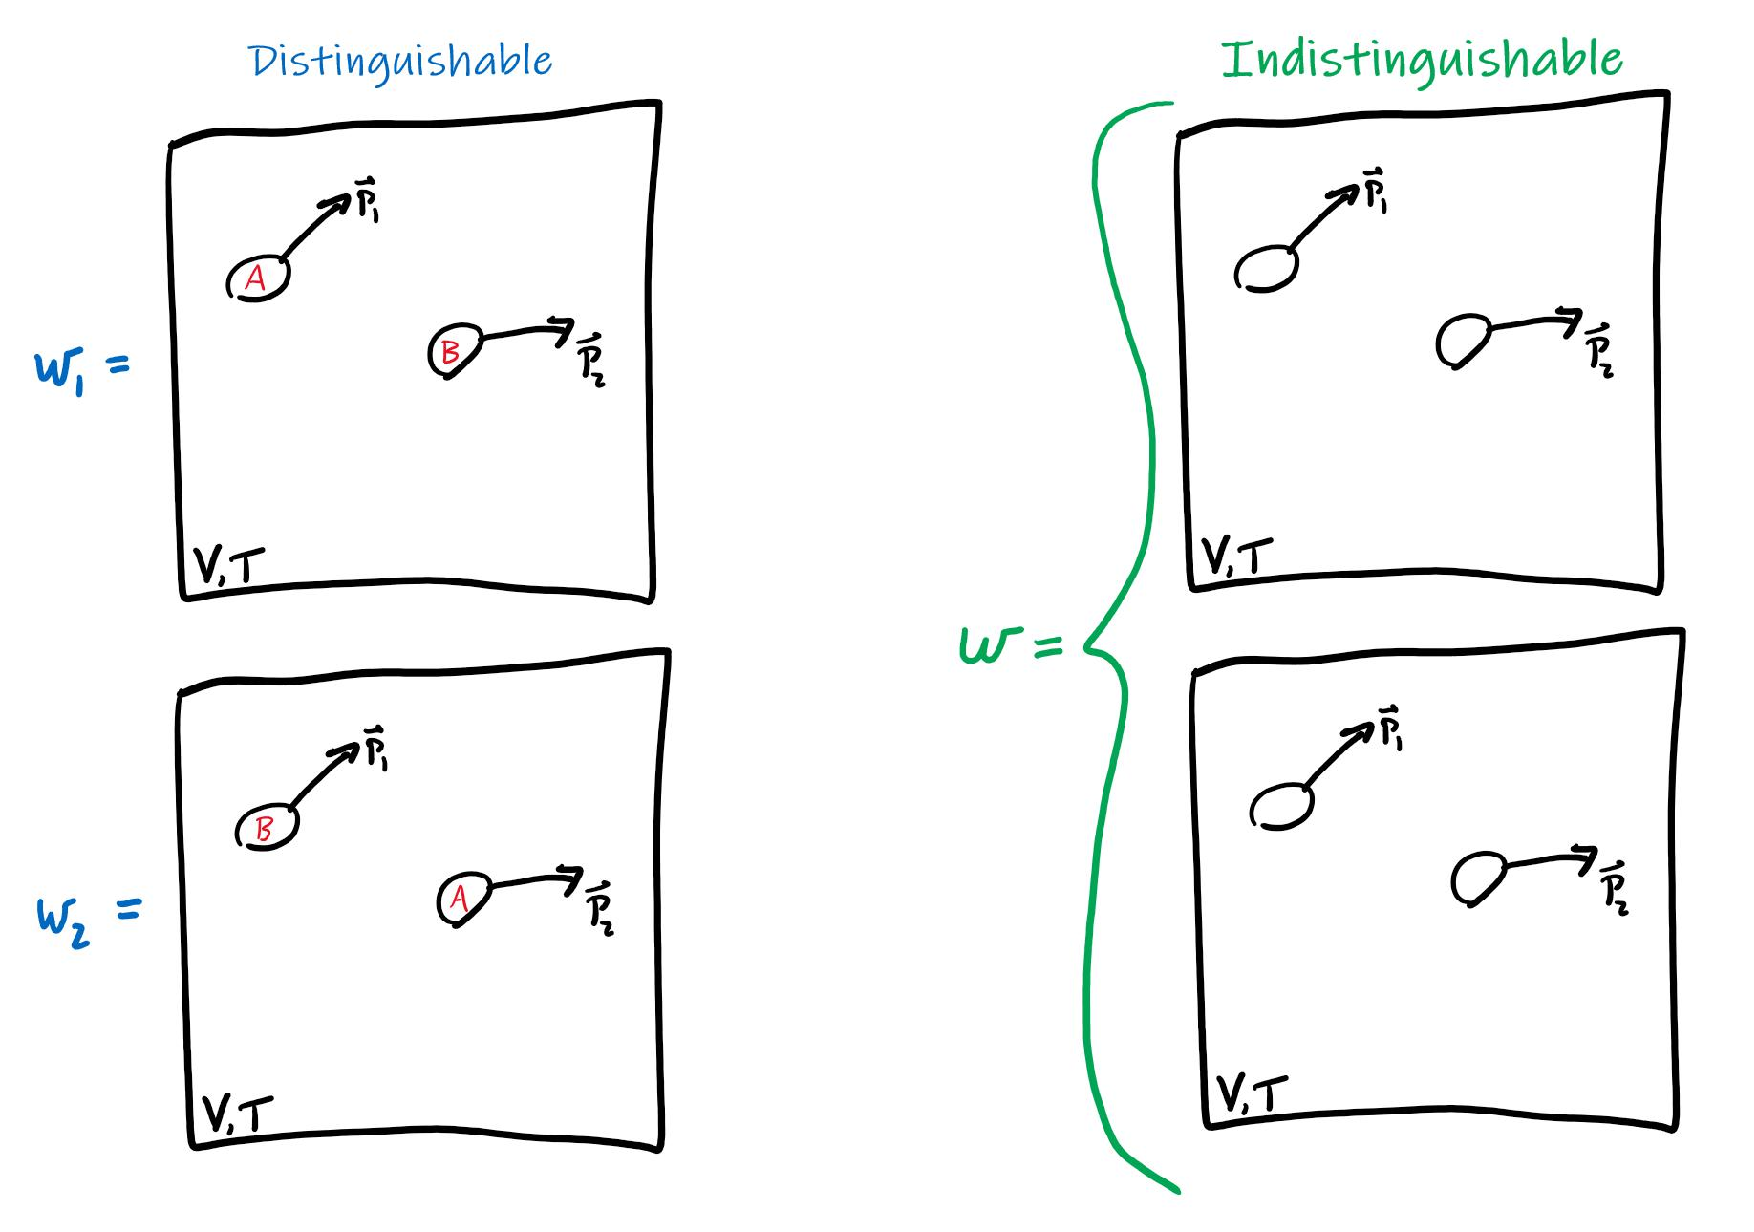
\includegraphics[width=1.0\textwidth]{figs/unit04_distinguish.pdf} % WARNING: ADJUSTED SIZE BY HAND TO FILL PAGE
\end{center}
If the particles are indistinguishable, no such labeling is possible, and there is only one micro-state for these $\left\{\vec p_1, \vec p_2\right\}$, rather than two.
This factor of $2$ is not accidental, as you can explore by counting how many micro-states there are for three distinguishable particles with momenta $\left\{\vec p_1, \vec p_2, \vec p_3\right\}$, compared to the single micro-state for the indistinguishable case:
\begin{mdframed}
  \ \\[100 pt]
\end{mdframed}

Generalizing to $N$ particles, we find that ideal gases with distinguishable particles have $N!$ times more micro-states compared to otherwise-identical ideal gases with indistinguishable particles: There are $N$ possible ways to label the particle with momentum $\vec{p}_1$, then $N - 1$ possible labels for $\vec{p}_2$, and so on.\footnote{This argument assumes the momenta themselves are distinguishable, $\vec{p}_i \neq \vec{p}_k$ for any $i \neq k$.  This is a reliable assumption for classical gases with $L\sqrt{mT} \gg \hbar$, but will need to be revisited when we consider quantum statistics.}
The partition function sums over these micro-states, but depends only on their energies, which are independent of any labeling.
Therefore this factor of $N!$ is the only difference between \eq{eq:ideal_dist} and the partition function for indistinguishable particles,
\begin{equation}
  \label{eq:ideal_indis}
  Z_I = \frac{1}{N!} \left(\frac{mTL^2}{2\pi\hbar^2}\right)^{3N / 2} = \frac{1}{N!} \left(\frac{L}{\lath}\right)^{3N} = \frac{1}{N!} \left(\frac{V}{\lath^3}\right)^N.
\end{equation}
% ------------------------------------------------------------------



% ------------------------------------------------------------------
\subsection{Internal energy, and entropy}
Now that we have the canonical partition function, let's apply our work from Unit~3 to predict the large-scale behaviour of the ideal gas it describes.
Our first targets are the average internal energy $\vev{E}$ and entropy $S$ for the gas, as functions of its fixed temperature $T$, conserved particle number $N$, and the volume $V = L^3$ of the box in which it is contained.
Let's begin with the slightly more complicated case of indistinguishable particles, \eq{eq:ideal_indis}.
Recalling the derivatives in Eqs.~\ref{eq:canon_entropy-F}--\ref{eq:canon_energy-F}, we should keep the temperature dependence explicit in our workings, rather than hidden inside the thermal de~Broglie wavelength $\lath(T)$.

By writing down the Helmholtz free energy,
\begin{equation*}
  F_I = -T \log Z_I = -\frac{3NT}{2}\log\left(\frac{mTL^2}{2\pi\hbar^2}\right) + T \log\left(N!\right),
\end{equation*}
we can quickly extract the internal energy,
\begin{equation*}
  \vev{E}_I = -T^2 \pderiv{}{T}\left(\frac{F_I}{T}\right) = -T^2 \pderiv{}{T}\left(-\frac{3N}{2}\log T + T\mbox{-independent}\right) = \frac{3}{2} NT.
\end{equation*}
This in turn provides the entropy
\begin{equation*}
  S_I = \frac{\vev{E}_I - F_I}{T} = \frac{3}{2} N + \frac{3N}{2}\log\left(\frac{mTL^2}{2\pi\hbar^2}\right) - \log\left(N!\right).
\end{equation*}
We can clean this up by reintroducing the thermal de~Broglie wavelength,
\begin{equation*}
  \frac{3N}{2}\log\left(\frac{mTL^2}{2\pi\hbar^2}\right) = \frac{3N}{2}\log\left(\frac{L^2}{\lath^2}\right) = N\log\left(\frac{V}{\lath^3}\right),
\end{equation*}
and by applying Stirling's formula to find
\begin{equation*}
  S_I = \frac{3}{2} N + N\log\left(\frac{V}{\lath^3}\right) - N\log N + N = \frac{5}{2} N + N\log\left(\frac{V}{N\lath^3}\right).
\end{equation*}
We can interpret $N\lath^3$ as the volume `occupied' by the $N$ particles. % TODO: Can revisit when introducing quantum statistics...

What are the corresponding results for the case of distinguishable particles, starting from \eq{eq:ideal_dist} for the partition function $Z_D$?
\begin{mdframed}
  $\displaystyle F_D = $ \\[50 pt]
  $\displaystyle \vev{E}_D = $ \\[50 pt]
  $\displaystyle S_D = $ \\[50 pt]
\end{mdframed}
You should find that the energy is the same whether or not we can label the particles:
\begin{equation}
  \label{eq:ideal_energy}
  \vev{E}_D = \vev{E}_I = \frac{3}{2} NT.
\end{equation}
This agrees with the argument in the previous section that multiplying $Z$ by a constant factor (here $N!$) does not change the internal energy expectation value.\footnote{The spin system we considered in \secref{sec:spin_info} behaved differently because its number of distinguishable micro-states per indistinguishable micro-state was the energy-dependent binomial coefficient $\binom{N}{n_+}$.  The energy dependence caused $Z_D$ vs.\ $Z_I$ to differ by more than a simple constant factor.}

However, the entropy reflects the extra information that distinguishability provides: % TODO: Could convert this into gap...
\begin{align}
  \label{eq:ideal_entropy}
  S_D & = \frac{3}{2} N + N \log\left(\frac{V}{\lath^3}\right) &
  S_I & = \frac{5}{2} N + N \log\left(\frac{V}{N\lath^3}\right).
\end{align}
The difference $S_I - S_D = N - N\log N \to -\log(N!) < 0$, meaning $S_I < S_D$, as expected.
We can also note that $\lath \to \infty$ as the temperature approaches absolute zero, $T \to 0$, apparently producing negative entropies for fixed $V$.
This is a warning sign that our classical assumptions are breaking down in this regime, and quantum effects would need to be taken into account.
% ------------------------------------------------------------------



% ------------------------------------------------------------------
\subsection{The mixing entropy and the `Gibbs paradox'}
In \secref{sec:heat_ex} we analysed what would happen if we allowed two micro-canonical systems to exchange energy, and then re-isolated them.
We saw that this procedure obeys the second law of thermodynamics --- the entropy never decreases, though we have to be careful to account for all of the entropy after re-isolating the two systems.

We can now carry out a similar thought experiment of allowing two \emph{canonical} systems to exchange \emph{particles}, and then re-separating them.
We demand that both canonical ensembles are in thermodynamic equilibrium with each other, for instance by sharing the same thermal reservoir with temperature $T$.
This procedure is illustrated below, where we simplify the setup by taking the two initial systems to have equal volumes, $V_A = V_B = V$, and numbers of particles, $N_A = N_B = N$. \\[-30 pt]
\begin{center}
  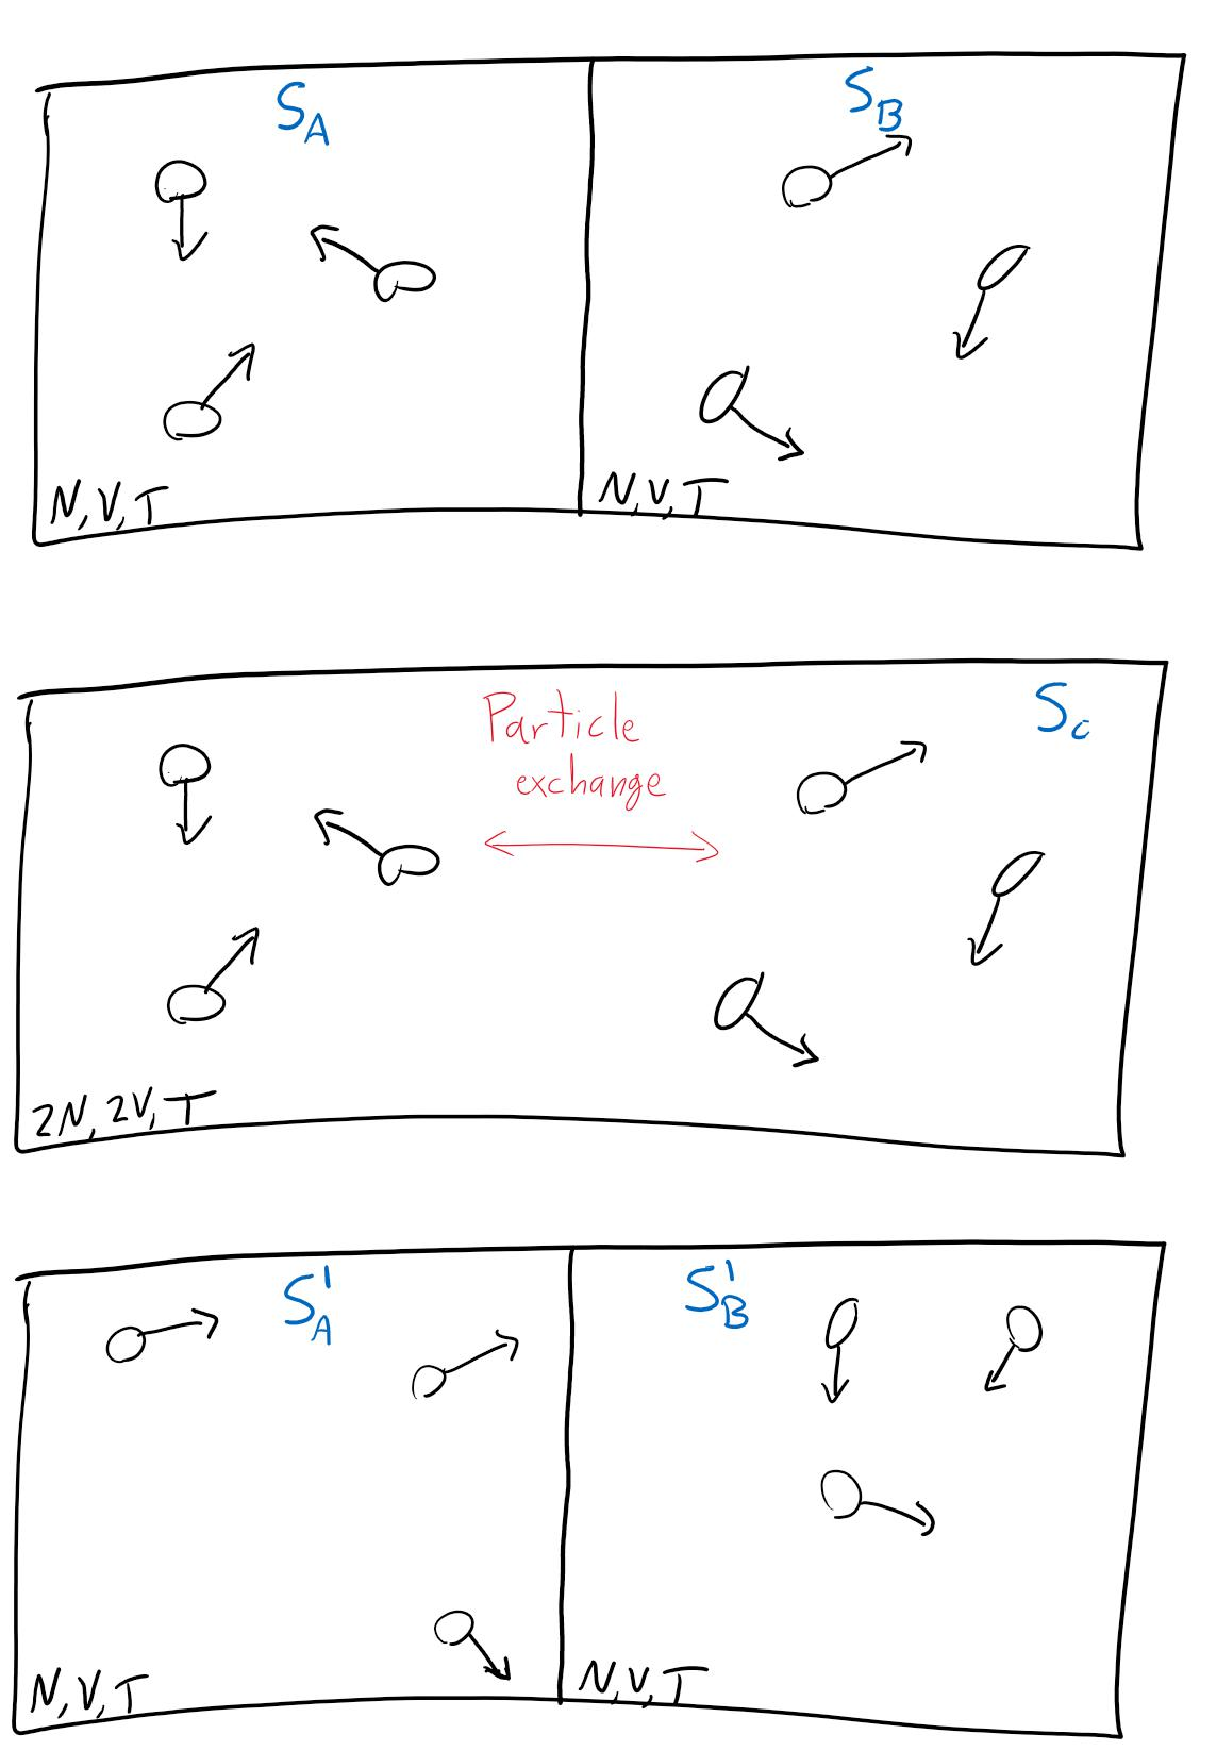
\includegraphics[width=0.64\textwidth]{figs/unit04_mixing.pdf} % WARNING: ADJUSTED SIZE BY HAND TO FIT ON PAGE
\end{center}

We can represent the process of combining and re-separating these systems as
\begin{equation*}
  \Om_A + \Om_B \lra \Om_C \lra \Om_A' + \Om_B'.
\end{equation*}
What is the entropy for each of these three stages?
Since the entropies depend on whether or not the particles in the gas are distinguishable from each other, let's first consider the case of \textit{indistinguishable} particles.

The initial entropy is the sum of the contributions from the two canonical systems, $S_A + S_B$, both of which are the same thanks to our simplification above:
\begin{mdframed}
  $\displaystyle S_A + S_B = $ \\[50 pt]
\end{mdframed}
To find the entropy $S_C$ of the combined system, we just need to consider what happens when we double the volume and also double the number of particles:
\begin{mdframed}
  $\displaystyle S_C = $ \\[50 pt]
\end{mdframed}
You should find $S_C = S_A + S_B$, which is consistent with the second law.

Things are more complicated when we re-separate the systems.
Analogously to our considerations in \secref{sec:heat_ex}, we need to sum over all the possible ways of dividing the $2N$ indistinguishable particles between the two re-separated boxes.
In particular, we need to perform this sum at the stage of computing the partition function $Z'$ for $\Om_A' + \Om_B'$, since this is the fundamental quantity from which the entropy is then derived as $S' = \pderiv{}{T}\left(T\log Z'\right)$. % Just like we computed the total number of micro-states when considering heat exchange in the micro-canonical context
In other words, we have to consider a logarithm of a sum rather than a sum of logarithms.

If $\nu$ particles end up in system $\Om_A'$, then the other system $\Om_B'$ must contain the remaining $2N - \nu$ particles, giving us
\begin{equation*}
  Z_{\nu} = \frac{1}{\nu!} \left(\frac{V}{\lath^3}\right)^{\nu} \times \frac{1}{(2N - \nu)!} \left(\frac{V}{\lath^3}\right)^{2N - \nu} = \frac{1}{\nu! \, (2N - \nu)!} \left(\frac{V}{\lath^3}\right)^{2N}.
\end{equation*}
Summing over all possible values of $0 \leq \nu \leq 2N$,
\begin{align*}
  & Z' = \sum_{\nu = 0}^{2N} Z_{\nu} = \left(\frac{V}{\lath^3}\right)^{2N} \sum_{\nu = 0}^{2N} \frac{1}{\nu! \, (2N - \nu)!} = \left(\frac{V}{\lath^3}\right)^{2N} \frac{1}{(2N)!} \sum_{\nu = 0}^{2N} \binom{2N}{\nu} \cr
  \implies & S_A' + S_B' = 2N \pderiv{}{T}\left(T\log \left[\frac{V}{\lath^3}\right]\right) - \log[(2N)!] + \log\left[\sum_{\nu = 0}^{2N} \binom{2N}{\nu}\right].
\end{align*}
This is a complicated expression.
In the 1870s, Gibbs introduced the following argument that helps to simplify it, which we will explore further in tutorials: For large $N \gg 1$, the entropy of the two subsystems is nearly saturated by the case in which the particles are divided roughly evenly between them, rather than being mostly in one of them.
Equivalently, there are far more micro-states with $N_A' \approx N_B' \approx N$, compared to all other terms in the sum above.

Therefore we can safely set $N_A' = N_B' = N$, which was already incorporated into the illustration above.\footnote{Formally this is only exact in the \textit{thermodynamic limit} $N \to \infty$, a concept we will discuss in Unit~9.}
This means $\Om_A' = \Om_A$ and $\Om_B' = \Om_B$, producing a final entropy of $S_A' + S_B' = S_A + S_B$ that satisfies the second law:
\begin{equation*}
  S_A' + S_B' = S_C = S_A + S_B.
\end{equation*}
This is just what we would expect from everyday experience: Opening a door between two identical rooms doesn't produce any observable effects, nor does reversing that process by closing the door.

Something interesting happens when we repeat this analysis for the case of \textit{distinguishable} particles, using our result for $S_D(N, V)$ in \eq{eq:ideal_entropy}.
If we consider the difference between the combined entropy $S_C$ and the initial entropy $S_A + S_B$,
\begin{align}
  \De S_{\mathrm{mix}} & = S_C - (S_A + S_B) = S_D(2N, 2V) - 2S_D(N, V) \cr
                       & = 3N + 2N \log\left(\frac{2V}{\lath^3}\right) - \left[3N + 2N \log\left(\frac{V}{\lath^3}\right)\right] = 2N\log 2 > 0, \label{eq:mixing_entropy}
\end{align}
we find the entropy increases upon combining the two initial systems.
This $\De S_{\mathrm{mix}} > 0$ is known as the \textbf{mixing entropy}.

This result $S_C > S_A + S_B$ is to be expected from the second law of thermodynamics.
However, repeating the argument above --- that we should have $N_A' \approx N_B' \approx N$ leading to $S_A' + S_B' = S_A + S_B$ after re-separating the systems --- would produce the prediction $S_A' + S_B' < S_C$, indicating a \textit{decrease} in the entropy by $\De S_{\mathrm{mix}}$ and an apparent violation of the second law.
This is known as the `Gibbs paradox', though Gibbs himself explained how a paradox is avoided. % `Paradoxes' in mathematical sciences typically indicate you've done something wrong...

The explanation is that because the particles are now distinguishable, $N_A' = N_A$ no longer suffices to establish $\Om_A' = \Om_A$ and $S_A' = S_A$.
Recovering $\Om_A$ would additionally require that the $N_A'$ particles in the re-separated system are the \emph{same} distinguishable particles that were initially in $\Om_A$.
While we can still expect $N_A' \approx N_B' \approx N$, the vast majority of the resulting micro-states will not correspond to micro-states of $\Om_A$ and $\Om_B$.
Summing over these additional possibilities ensures $S_A' + S_B' > S_A + S_B$, and it turns out $S_A' + S_B' \geq S_C$ as well, obeying the second law of thermodynamics.

These thought experiments provide another example of behaviour that depends on the intrinsic information content of the system --- whether or not the particles in an ideal gas can be distinguished from each other in principle.
Mixing gases of distinguishable particles introduces a positive mixing entropy, \eq{eq:mixing_entropy}, but for gases of indistinguishable particles there is no change in entropy when we let two subsystems mix, or when we reverse that process and re-separate them.
Due to the second law, processes that produce an increase in entropy are \href{https://en.wikipedia.org/wiki/Irreversible_process}{irreversible}. % Could connect this to the illustration of diffusion of dye in water from the first lecture
% ------------------------------------------------------------------



% ------------------------------------------------------------------
\subsection{\label{sec:ideal_gas}Pressure, ideal gas law, and equations of state}
Below \eq{eq:ideal_dist} we emphasized that the ideal gas partition function depends on the volume of the gas, $V$, in addition to the fixed temperature $T$ and conserved particle number $N$ that always characterize systems governed by the canonical ensemble.
Parameters like $V$ that appear in the partition function are called \textbf{control parameters}, with the idea that they can (in principle) be controlled in experiments.
Control parameters generally enter the partition function through the definition of the energies $E_i$ for the micro-states $\om_i$.
Another example is the magnetic field strength $H$ for the spin systems we considered earlier.

Focusing on ideal gases for now, we see that all dependence on $V$ drops out in our results for the average internal energy, \eq{eq:ideal_energy}.
On the other hand, the entropies in \eq{eq:ideal_entropy} do depend on the volume.
For both cases of distinguishable and indistinguishable particles, the entropy $S$ depends on the same combination of volume and temperature: $V \lath^{-3} \propto V T^{3/2}$.
If we keep $N$ fixed and consider using our experimental control to change the volume and the temperature of the system, the entropy will typically change as a consequence, unless the following relation is satisfied:
\begin{equation*}
  V T^{3/2} = \mbox{constant} \qquad \implies \qquad S = \mbox{constant.}
\end{equation*}

Such \textbf{constant-entropy (or isentropic) processes} will be important in our upcoming analyses of thermodynamic cycles.\footnote{The term \emph{isentropic} is based on the Greek word $\iota\sigma o\varsigma$ (``isos''), meaning ``equal''.}
These cycles will involve making changes to control parameters, which is a topic we have already started to consider through the micro-canonical temperature (\eq{eq:temperature}) and the canonical heat capacity (\eq{eq:heat_cap}).
The pressure of an ideal gas is similarly connected to a change in its volume, which we can motivate by thinking about squeezing an inflated balloon into a small box.

\begin{shaded}
  The \textbf{pressure} is defined to be
  \begin{equation}
    \label{eq:pressure}
    P = -\left. \pderiv{}{V} \vev{E}\right|_S,
  \end{equation}
  with constant entropy $S$.
  In words, the pressure is the isentropic response of the system's internal energy to a change in its volume.
\end{shaded}

In Unit~5 we will look in detail at processes that change some or all of the pressure, volume, temperature, or internal energy of an ideal gas, with $N$ fixed.
Although changing the temperature departs from the assumptions of the canonical ensemble, we will be able to analyse such a process as a change from one canonical system (in thermodynamic equilibrium with a thermal reservoir that fixes the initial temperature $T_0$) to another (in thermodynamic equilibrium with a different thermal reservoir that fixes the final temperature $T_f$).

If we consider an isentropic process with $N$ fixed, then the temperature and volume are related,
\begin{equation*}
  V T^{3/2} = c^{3/2} \qquad \lra \qquad T = c V^{-2 / 3},
\end{equation*}
with $c$ a constant.
By inserting this into \eq{eq:ideal_energy}, we can relate the average internal energy to the volume,
\begin{equation*}
  \vev{E} = \frac{3}{2} NT = \frac{3c}{2} N V^{-2 / 3} \qquad \mbox{for constant entropy}.
\end{equation*}
Using this constant-entropy expression, what is the pressure for the ideal gas?
\begin{mdframed}
  $\displaystyle P = -\left. \pderiv{}{V} \vev{E}\right|_S = $ \\[100 pt]
\end{mdframed}

\begin{shaded}
  You should find the \textbf{ideal gas law},
  \begin{equation}
    \label{eq:ideal_gas_law}
    PV = NT,
  \end{equation}
  which is an example of an \textbf{equation of state}.
\end{shaded}

The ``state'' referred to by this terminology is different from the micro-states that we have mostly discussed up until now.
Whereas each micro-state is defined by detailed information about the microscopic degrees of freedom that constitute the system, this \textbf{macro-state} concerns only the large-scale (\textit{macroscopic}) properties of the system, such as its pressure, volume, temperature, entropy, or internal energy.
(Macro-states are sometimes called ``system states'' or ``thermodynamic states''.)
Equations of state are relations between these large-scale properties.

Historically, equations of state were observed empirically and studied experimentally well before the mathematical development of statistical mechanics.
In the 1660s, for instance, \href{https://en.wikipedia.org/wiki/Robert_Boyle}{Robert Boyle} experimented with changing the pressure of a gas while holding its temperature fixed, finding a special case of the ideal gas law,
\begin{equation*}
  PV = \mbox{constant} \qquad\qquad \mbox{for constant } N \mbox{ and } T,
\end{equation*}
which became known as ``\href{https://en.wikipedia.org/wiki/Boyle's_law}{Boyle's law}''.
(I include the quotation marks to emphasize the limitations of assigning an individual sole credit for advances arising from the work of broad scientific communities.)

Other equations of state reflecting different aspects of the ideal gas law were uncovered during the Industrial Revolution:
 \\[-24 pt]
\begin{itemize}
  \item $\displaystyle \frac{V}{T} = \mbox{constant}$ \qquad\qquad for constant $N$ and $P$ (1787, ``\href{https://en.wikipedia.org/wiki/Charles's_law}{Charles's law}'') %, attributed to \href{https://en.wikipedia.org/wiki/Jacques_Charles}{Jacques Charles}
  \item $\displaystyle \frac{P}{T} = \mbox{constant}$ \qquad\qquad for constant $N$ and $V$ (1802, ``\href{https://en.wikipedia.org/wiki/Gay-Lussac's_law}{Gay-Lussac's law}'') %, attributed to \href{https://en.wikipedia.org/wiki/Joseph_Louis_Gay-Lussac}{Joseph Gay-Lussac}
  \item $\displaystyle \frac{V}{N} = \mbox{constant}$ \qquad\qquad for constant $P$ and $T$ (1812, ``\href{https://en.wikipedia.org/wiki/Avogadro's_law}{Avogadro's law}'') %, attributed to \href{https://en.wikipedia.org/wiki/Amedeo_Avogadro}{Amedeo Avogadro}
\end{itemize}
In the 1830s \href{https://en.wikipedia.org/wiki/Benoit_Paul_Emile_Clapeyron}{\'Emile Clapeyron} combined these empirical results into the ideal gas law itself, which \href{https://en.wikipedia.org/wiki/August_Kroenig}{August Kr{\"o}nig} and \href{https://en.wikipedia.org/wiki/Rudolf_Clausius}{Rudolf Clausius} independently derived on the basis of statistical mechanics in the 1850s.
These historical considerations are useful to illustrate how progress in scientific and mathematical understanding went hand-in-hand with industrial developments, including the design of engines and related machines, which are connected to our next topic of thermodynamic cycles.
% ------------------------------------------------------------------


\newpage
% ------------------------------------------------------------------
\renewcommand{\thisunit}{MATH327 Unit 5}
\renewcommand{\moddate}{Last modified 4 Mar.~2025}
\setcounter{section}{5}
\setcounter{subsection}{0}
\phantomsection
\addcontentsline{toc}{section}{Unit 5: Thermodynamic cycles}
\section*{Unit 5: Thermodynamic cycles}
\subsection{\label{sec:work}Work, pressure and force}
In the previous section we defined the pressure of an ideal gas in the canonical ensemble as the thermodynamic response of the internal energy to an isentropic change in the volume (\eq{eq:pressure}).
We motivated this definition by thinking about `squeezing' the system --- exerting a force on it --- which suggests a connection between pressure and force.
Here we make this connection explicit by considering how the energy of an object changes when a force acts on it.

Let's begin by considering a single object at position $\vec r = (x, y, z)$, which is displaced by a vector $\d{\vec r}$ due to a force $\vec F(\vec r)$.
The \emph{work} done by this force is defined to be the resulting change in the energy of the object.
Infinitesimally, $W = \d{E} = \vec F\cdot \d{\vec r}$, which generalizes to the line integral $W = \De E = \int \vec F(r)\cdot d\vec r$.

A famous example is an object falling due to the force of the Earth's gravity.
That force is $\vec F = (0, 0, -mg)$, where $m$ is the mass of the object, $g \approx 9.8~\mathrm{m}/\mathrm{s}^2$ (metres per second per second) is the strength of gravity near the surface of the Earth, and the negative sign indicates that the gravitational force is directed downward.
Suppose the object starts from rest, with initial kinetic energy $E_0 = 0$, and falls downward, parallel to $\vec F$, from a height $h$.
Its final energy $E_f$ upon hitting the ground comes from the work done by the Earth's gravity:
\begin{align*}
  W & = \int \vec F(r)\cdot d\vec r = -mg \int_h^0 dz = mgh > 0 \\
  E_f & = E_0 + \De E = 0 + W = mgh = \frac{p_z^2}{2m} \qquad \lra \qquad p_z = -m\sqrt{2gh},
\end{align*}
where \eq{eq:momentum} relates the energy to the momentum $\vec p = (p_x, p_y, p_z)$.

\begin{shaded}
  Generalizing to $N \gg 1$ objects in a statistical system governed by the canonical ensemble, we define the \textbf{work} done by a force to be the resulting change in the system's average internal energy \textit{due to that force}, $W = \De\!\vev{E}_{\text{force}}$.
  In practice, the volume is the control parameter that such a force will change.
\end{shaded}

This change in $\vev{E}$ due to a change in volume suggests that the work is related to the pressure defined by \eq{eq:pressure}.
We can formalize this relation by considering the setup shown below (from Schroeder's \textit{Introduction to Thermal Physics}). \\[-24 pt]
\begin{center}
  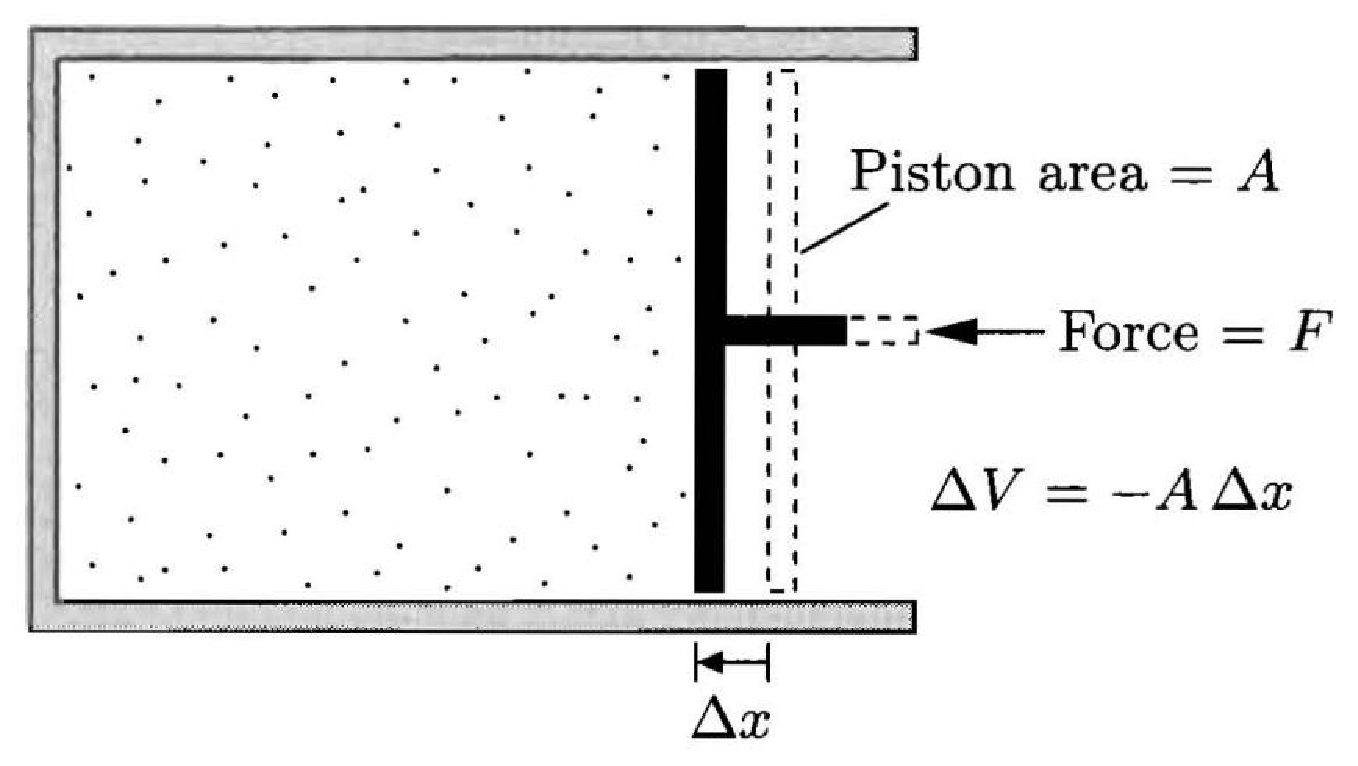
\includegraphics[width=0.54\textwidth]{figs/unit05_piston.pdf} % WARNING: ADJUSTED SIZE BY HAND TO FIT ON PAGE
\end{center}

Here we have an ideal gas in a container of volume $V$, with one wall of that container being a piston that we can move by applying a force $F$.
Let's demand that this process leaves the entropy of the gas constant.
The displacement $\De x > 0$ shown in the figure reduces the volume of the gas, by $\De V = -A\De x < 0$ where $A$ is the surface area of the piston.
Since the force $F$ is parallel to the piston's displacement $\De x$, it does positive work $W = F\De x > 0$.
Therefore the internal energy of the gas increases by $\De\!\vev{E} = W$, at the same time as its volume decreases isentropically, so from \eq{eq:pressure}
\begin{equation}
  P = -\left. \pderiv{}{V} \vev{E}\right|_S = -\frac{W}{\De V} = \frac{F\De x}{A\De x} = \frac{F}{A}.
\end{equation}
This identifies the pressure of an ideal gas in a container as the force per unit area that the gas exerts on the container wall, in agreement with our everyday experiences.

Rearranging the expressions above, we can obtain an expression for the work \textit{done on the gas by its surroundings} --- that is, by the external force applied to move the piston and change the volume.
Still assuming a constant-entropy (isentropic) process, this input work must match the increase in the gas's average internal energy,
\begin{align*}
  W & = \De\!\vev{E} = -P \De V & & \mbox{for constant entropy.}
\end{align*}
If the entropy is allowed to change, this relation between work and pressure will still hold.
However, as we will see in the next section, the non-constant entropy will introduce an additional change in the average internal energy unrelated to a force, leading to $W \neq \De\!\vev{E}$ and leaving only the relation
\begin{align}
  \label{eq:work_constP}
  W & = -P \De V & & \mbox{more generally.}
\end{align}
Later we will be interested in thermodynamic engines where work is \textit{done by the gas on its surroundings}.
This removes energy from the gas, corresponding to a negative $W < 0$, and we will need to be careful to keep track of the negative signs and their physical meaning.

Of course, as we change the volume of the gas, the pressure itself may change as described by the gas's equation of state --- such as the ideal gas law, \eq{eq:ideal_gas_law}.
In all these considerations we will keep the particle number $N$ fixed, though in principle it could change in the same way as discussed below \eq{eq:pressure} for the temperature.
With the equation of state providing an expression $P(V)$ for the pressure as a function of the volume, \eq{eq:work_constP} generalizes to
\begin{equation}
  \label{eq:work}
  W = -\int_{V_0}^{V_f} P(V) \d{V}.
\end{equation}
% ------------------------------------------------------------------



% ------------------------------------------------------------------
\subsection{Heat and entropy}
Now let's switch things up by changing the temperature $T$ of an ideal gas while keeping its volume $V$ and particle number $N$ constant.
Since the volume is constant, \eq{eq:work} indicates that no work is done, $W = 0$.
Even so, from \eq{eq:ideal_energy} we have $\vev{E} = \frac{3}{2} NT$ and can see that the average internal energy still changes,
\begin{equation}
  \label{eq:dE_dT}
  \d{\!\vev{E}} = \frac{3}{2} N \d{T}.
\end{equation}

In order to remain consistent with our discussion in the previous section, we should expect a change in the entropy to accompany this change in the internal energy that occurs with no work done.
Indeed, both distinguishable and indistinguishable particles lead to the same the temperature dependence in \eq{eq:ideal_entropy} for the entropy:
\begin{equation*}
  S = N\log\left(\lath^{-3}\right) + T\mbox{-independent} = N\log\left(T^{3 / 2}\right) + T\mbox{-independent}.
\end{equation*}
What is the change in entropy that results from changing the temperature by $dT$?
\begin{mdframed}
  $\displaystyle \d{S} = $ \\[50 pt]
\end{mdframed}
Looking back to \eq{eq:dE_dT}, you should find $\d{\!\vev{E}} = T \d{S}$, which leads us to another important definition.

\begin{shaded}
  The \textbf{heat} added to or removed from a statistical system is defined to be
  \begin{equation}
    \label{eq:heat_def}
    Q = T \d{S},
  \end{equation}
  and corresponds to the change in the average internal energy of the system when the volume and particle number are kept constant.
\end{shaded}

In the same way as our considerations of the work $W$ in the previous section, we can generalize this infinitesimal definition to
\begin{equation}
  \label{eq:heat}
  Q = \int_{S_0}^{S_f} T(S) \d{S},
\end{equation}
with $Q = \De\!\vev{E}$ when the volume is constant.
Here we assume it is possible to invert the usual canonical relation that expresses the entropy as a function of the temperature, $S(T)$.
Some textbooks may refer to infinitesimal heat and work as ``$\d{Q}$'' and ``$\d{W}$'', but this notation can easily be misinterpreted as describing a `change' in heat or work.
Instead, heat and work are themselves changes in the internal energy.

Like the work $W$, the heat $Q$ is positive when energy is added to the system to increase $\vev{E}$, and negative when energy is removed.
Recalling that the canonical ensemble involves placing the system in thermal contact with a large external thermal reservoir, we can recognize that this energy is not being created or destroyed, but is instead flowing back and forth between the system and the reservoir.
When considering heat, we will also demand that no \emph{entropy} is created or destroyed --- a positive $\d{S}$ will indicate entropy flowing into the system from the reservoir, while a negative value reflects entropy moving from the system to the reservoir.
Because the total entropy of the system plus its reservoir is constant, these processes are reversible, making it possible for the system to return to its starting macro-state.\footnote{In the case of irreversible processes, there must be sources of entropy creation, which change \eq{eq:heat_def} to $Q < T \d{S}$.  The \href{https://en.wikipedia.org/wiki/Clausius_theorem}{Clausius inequality} $Q \leq T \d{S}$ covers both reversible and irreversible cases.}

We have already considered isentropic processes with $\d{S} = 0$, for example in the definition of pressure in \eq{eq:pressure}.
With our assumption of reversibility, the definition of heat provides a new perspective on such processes:

\begin{shaded}
  We define an \textbf{adiabatic} process to be a change in the control parameters of a system that occurs without transferring heat, $Q = 0$.
  When this process is reversible, \eq{eq:heat_def} guarantees that it also does not change the system's entropy.
\end{shaded}

Since the canonical ensemble requires thermal contact between the system and its surroundings, the practical way to avoid heat exchange is to change the control parameters quickly.
That is, \textbf{adiabatic processes are fast} enough that the system does not have time to exchange heat (and hence entropy) with its surroundings.
The opposite extreme would be a process slow enough that any and all possible heat exchange can be completed while it is underway.
Based on our work in \secref{sec:heat_ex}, we can see that such heat exchange will keep the system's temperature equal to the temperature of its surroundings.
Taking that surrounding temperature to be constant, we reach the conclusion that \textbf{constant-temperature (or isothermal) processes are slow}.
Real processes generally exist in between these two extremes, usually closer to the adiabatic limit.
% ------------------------------------------------------------------



% ------------------------------------------------------------------
\subsection{Thermodynamic cycles}
Now we can generalize our considerations in the previous two sections to address simultaneous changes in the temperature $T$ and the volume $V$ of an ideal gas, still with fixed particle number $N$.
We are used to working with the internal energy $\vev{E}\!(T, V)$ and entropy $S(T, V)$ as functions of the temperature and volume.
Inverting the latter relation allows us to instead express the temperature $T(S, V)$ as a function of the entropy and volume, which carries through to the internal energy $\vev{E} = \frac{3}{2}NT$,
\begin{equation*}
  \vev{E}\!(T, V) \ \to \ \vev{E}\!(S, V).
\end{equation*}
Let's expand this to first order in a multi-variable Taylor expansion:
\begin{equation*}
  \vev{E}\!(S, V) \approx \vev{E}\!(S_0, V_0) + (S - S_0) \left.\pderiv{\vev{E}}{S}\right|_V + (V - V_0) \left.\pderiv{\vev{E}}{V}\right|_S.
\end{equation*}
This approximation becomes exact in the limit of infinitesimal changes
\begin{align*}
  \vev{E}\!(S, V) - \vev{E}\!(S_0, V_0) & \to \d{\!\vev{E}} \qquad &
  S - S_0 & \to \d{S} \qquad &
  V - V_0 & \to \d{V}. &
\end{align*}
At the same time, we can recognize the temperature from \eq{eq:temperature} and the (negative) pressure from \eq{eq:pressure}, to obtain
\begin{equation}
  \label{eq:first_law}
  d\!\vev{E} = T \d{S} - P \d{V} = Q + W.
\end{equation}
This is a generalized form of the \textbf{first law of thermodynamics}: Any change in the internal energy of a canonical system must be matched by (either or both) heat exchange with its surroundings or work done by or on those surroundings.

\begin{shaded}
  We now have all the concepts and \textbf{key equations} needed to consider a variety of ways to manipulate a canonical, classical, non-relativistic ideal gas in a container: \\[-24 pt]
  \begin{itemize}
    \item \eq{eq:ideal_energy} for the internal energy: \hfill $\vev{E} = \frac{3}{2} NT$
    \item \eq{eq:ideal_entropy} for the condition of constant entropy: \hfill $V T^{3/2} = \mbox{constant}$
    \item \eq{eq:ideal_gas_law} for the equation of state (ideal gas law): \hfill $PV = NT$
    \item \eq{eq:first_law} for the first law of thermodynamics: \hfill $d\!\vev{E} = T \d{S} - P \d{V} = Q + W$
  \end{itemize}
\end{shaded}

As examples of manipulations we can carry out by changing the system's control parameters, the piston we considered in \secref{sec:work} allows us to compress or expand the gas.
This change in volume could be fast to keep the entropy constant (adiabatic), or slow to keep the temperature constant (isothermal).
Alternatively, we can clamp the piston in place to keep the volume constant, and add heat to the gas to increase its temperature --- according to the ideal gas law, this will also increase the pressure of the gas.
Or we can add heat while keeping the pressure constant by applying a constant force to the piston.
The ideal gas law then implies the volume will increase, pushing out the piston and potentially doing work on the surroundings.

It's possible to carry out a sequence of such manipulations that cause the system to end up in the same thermodynamic (macro-)state in which it started, with the same pressure, volume, temperature and internal energy. % TODO: Could comment that this is related to our assumption of reversibility...
This sequence can then be repeated over and over again, always returning to the same starting point.
Such a repeatable process is known as a \textbf{thermodynamic cycle}.
As we will see in the next section, these cycles can make use of heat to have the system do work on its surroundings (providing an \textit{engine}), or make use of work to remove heat from the system (providing a \textit{refrigerator}), among other applications.

With $N$ fixed, the key equations above allow us to specify the full macro-state for an ideal gas solely in terms of the pressure $P$ and the volume $V$.
The ideal gas law provides the temperature $T = \frac{PV}{N}$, which then determines the internal energy $\vev{E} \propto NT$.
This makes it convenient to represent the system's macro-state as a point in a \textbf{pressure--volume} (or $\mathbf{PV}$) \textbf{diagram} --- a graph with the volume on the horizontal axis and the pressure on the vertical axis.
The manipulations discussed above correspond to lines in $PV$~diagrams.
In the case of a thermodynamic cycle, the lines must meet up to form a closed path for the system to go around as the cycle is repeated.

For example, the left figure on the next page shows the $PV$~diagram for isothermal expansion of the gas, which is slow enough for heat to enter the system to keep the temperature fixed despite the expansion.
\begin{center} % Don't need centering, but this will provide consistent vertical spacing
  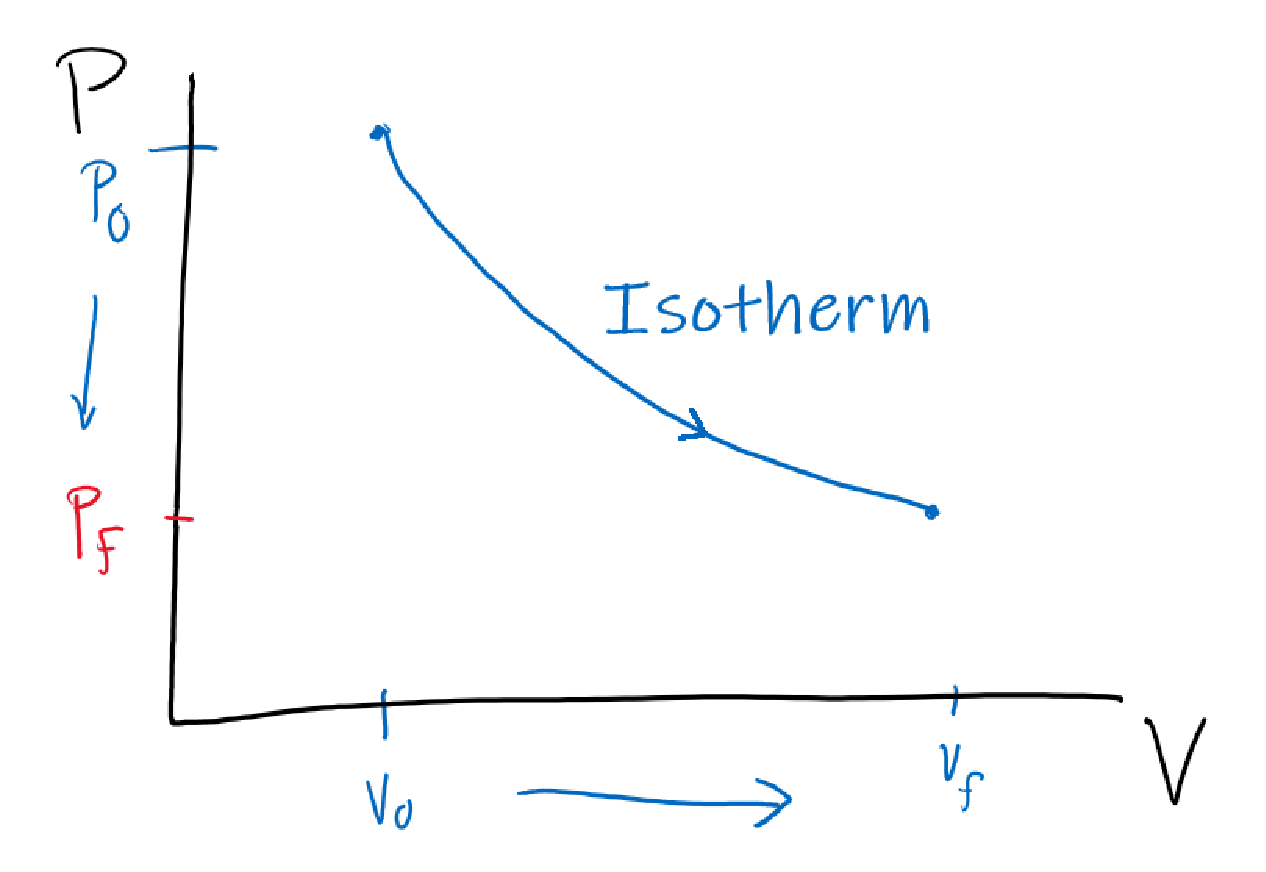
\includegraphics[width=0.475\textwidth]{figs/unit05_isotherm.pdf}\hfill 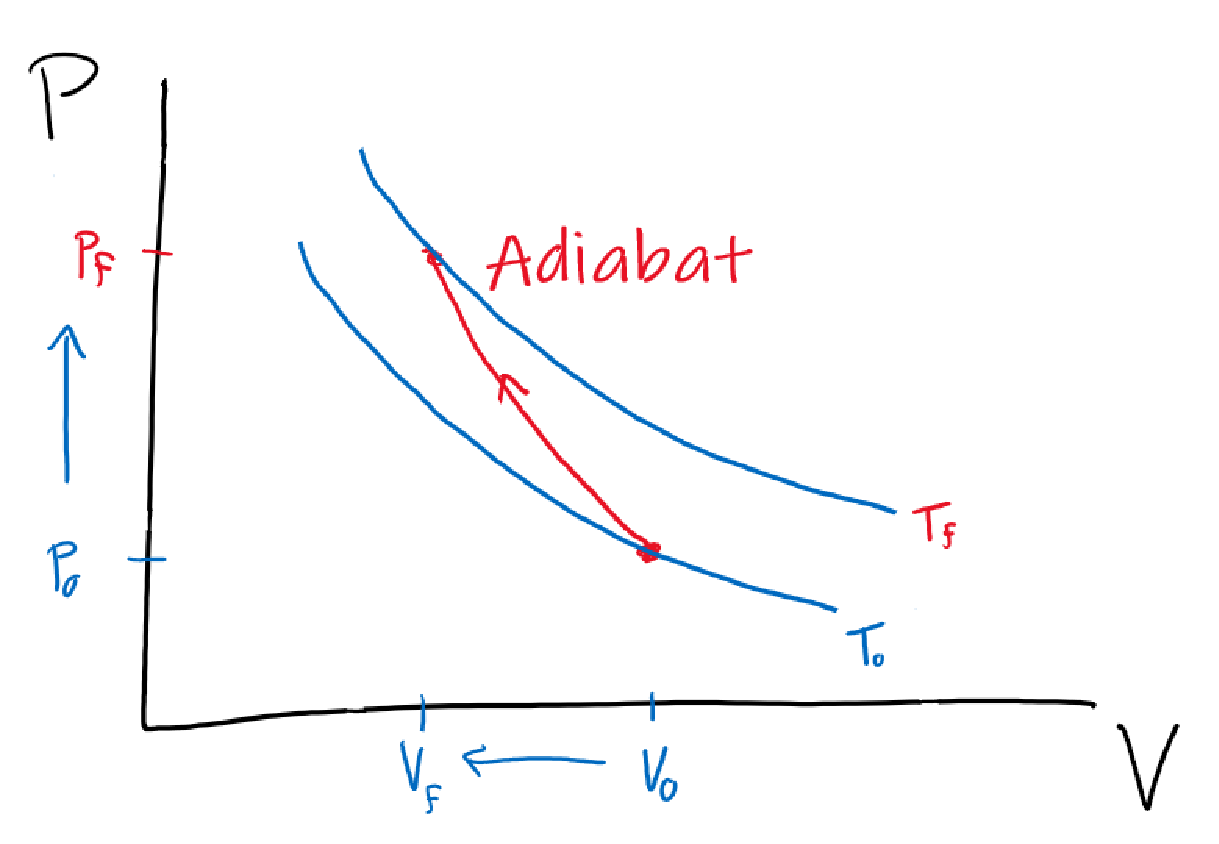
\includegraphics[width=0.475\textwidth]{figs/unit05_adiabat.pdf}
\end{center}
The line in a $PV$~diagram for an isothermal process is known as an \textit{isotherm}.
As the volume expands from $V_0$ to $V_f$, the temperature (and therefore $PV$) is constant.
What is the change in pressure $\De P = P_f - P_0$ in terms of $P_0$, $V_0$ and $V_f$?
What would it mean if two isotherms were to cross in a $PV$~diagram?
\begin{mdframed}
  \ \\[100 pt]
\end{mdframed}

Similarly, we can consider the $PV$~diagram on the right for adiabatic compression of the gas, which occurs too quickly for heat to be exchanged.
In this case both the pressure and temperature change, while the entropy (and therefore $VT^{3 / 2}$) is constant.
What are $\De P$ and the change in the temperature $\De T = T_f - T_0$ in terms of $P_0$, $V_0$, $V_f$ and the fixed number of particles $N$?
Can you convince yourself that two distinct reversible adiabats never cross? % physics.stackexchange.com/a/427582/34991 --- both adiabats intersect isotherms, but getting back to same entropy around cycle forbids heat flow to keep temperature constant on that isotherm
\begin{mdframed}
  \ \\[120 pt]
\end{mdframed}
% ------------------------------------------------------------------



% ------------------------------------------------------------------
\subsection{The Carnot cycle}
A famous thermodynamic cycle was proposed by \href{https://en.wikipedia.org/wiki/Nicolas_Leonard_Sadi_Carnot}{Sadi Carnot} in 1824, and laid the groundwork for subsequent development of engines and refrigerators later in the nineteenth century.
The key idea is to propose that the ideal gas in its container can exchange energy with either of \emph{two} different thermal reservoirs: a hot reservoir with a higher temperature $T_H$ and a cold reservoir with a lower temperature $T_L$. % Note 'C' reserved to refer to a point on the PV diagram below
The Carnot cycle consists of four stages, which are first shown below in the form of a $PV$~diagram, then illustrated in a sketch (adapted from Schroeder's \textit{Introduction to Thermal Physics}) that provides a more concrete picture of the physical processes, and finally summarized in words.

\begin{center}
  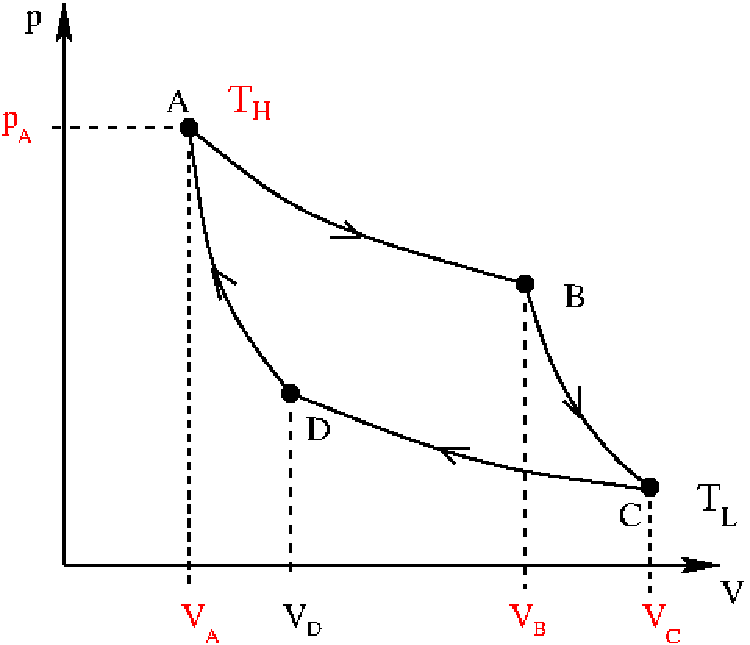
\includegraphics[width=0.75\textwidth]{figs/unit05_carnot-PV.pdf} \\[36 pt]
  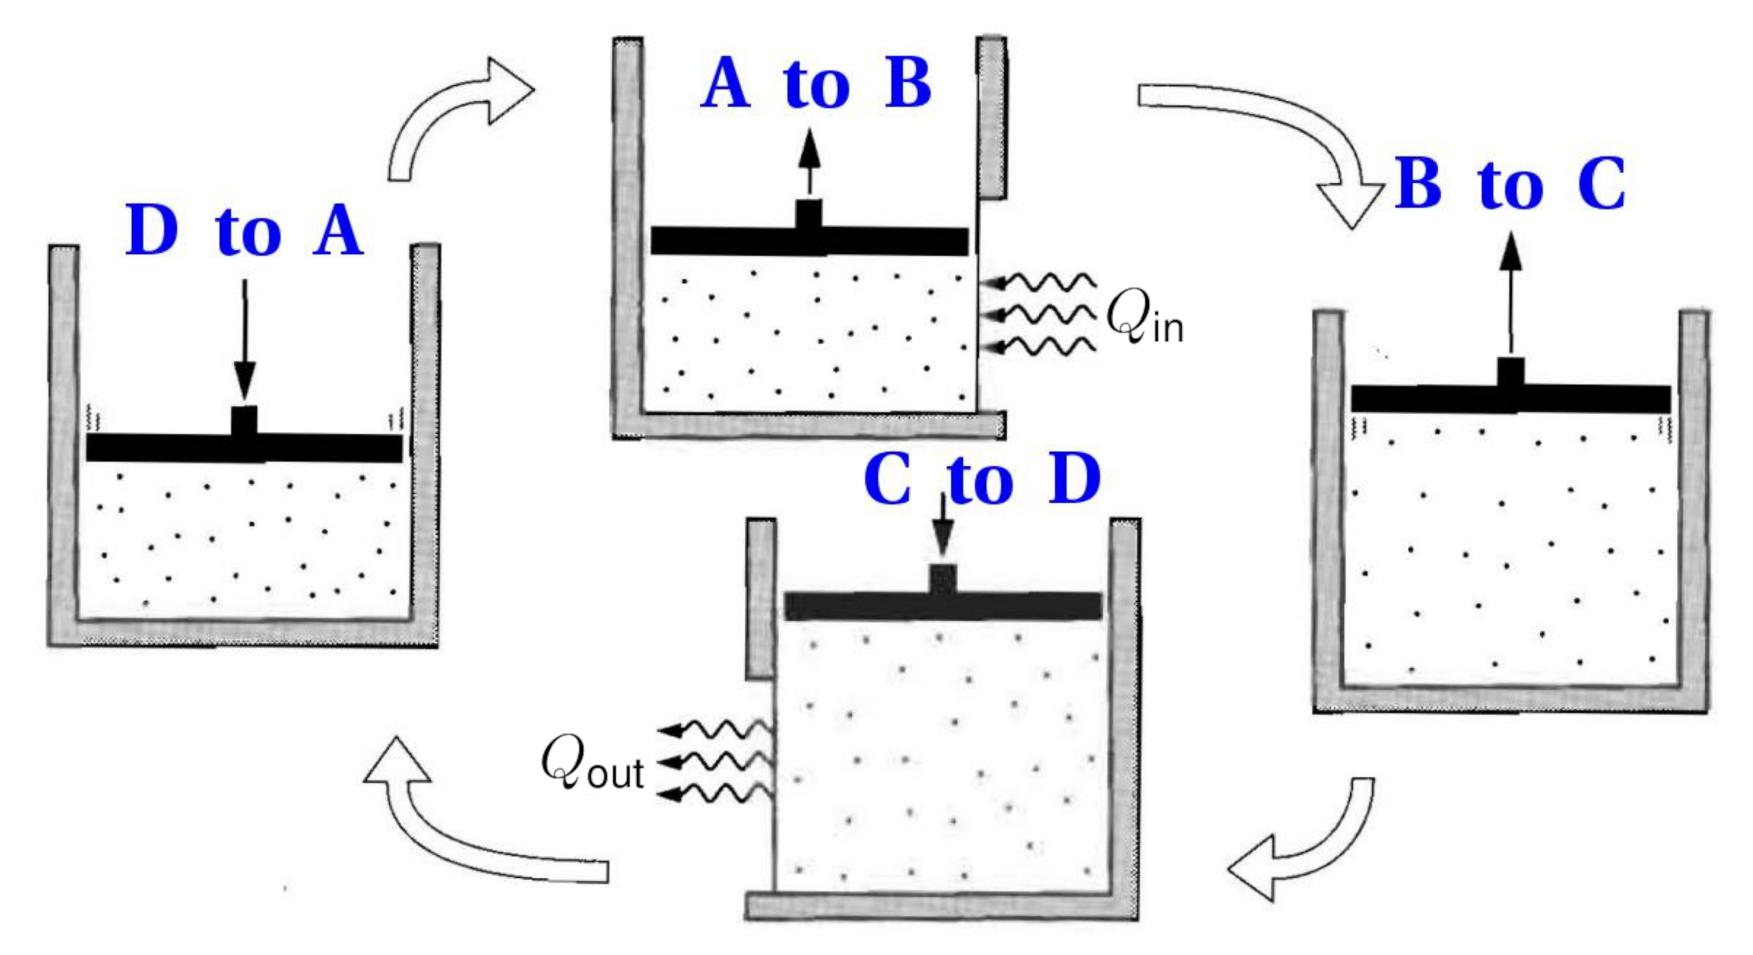
\includegraphics[width=\textwidth]{figs/unit05_carnot.pdf}
\end{center}

The illustration above supposes that the hot reservoir is located to the right of the system, while the cold reservoir is on its left.
In words, the four stages are the following: \\[-24 pt]
\begin{itemize}
  \item From point $A$ to point $B$ the system undergoes slow isothermal expansion, bringing in heat $Q_{\text{in}}$ from the hot reservoir in order to keep its temperature $T_H$ fixed.
  \item From point $B$ to point $C$ the system undergoes fast adiabatic expansion, with no heat exchange, until its temperature falls from $T_H$ down to $T_L$.
  \item From point $C$ to point $D$ the system undergoes slow isothermal compression, expelling heat $Q_{\text{out}}$ into the cold reservoir to keep its temperature $T_L$ fixed.
  \item From point $D$ to point $A$ the system undergoes fast adiabatic compression, with no heat exchange, until its temperature rises from $T_L$ back up to $T_H$.
\end{itemize}

We need to make sure that these processes really do produce a self-consistent closed cycle that our system could repeatedly follow.
In a real experiment, we would have full control over the four input variables $\left\{P_A, V_A, V_B, V_C\right\}$ coloured red in the $PV$~diagram above. % Could alternatively control temperatures...
Specifically, we can prepare our $N$-particle system in initial macro-state $A$ with our choice of pressure $P_A$ and volume $V_A$, which sets the higher temperature $T_H = \frac{P_A V_A}{N}$ of the hot reservoir.
We can then freely choose the volume $V_B > V_A$ at which to switch from isothermal expansion to adiabatic expansion, and similarly choose the volume $V_C > V_B$ at which we stop expanding and start compressing.
These choices of $V_B$ and $V_C$ set the lower temperature $T_L$ of the cold reservoir.

At this point, however, we are no longer free to choose an arbitrary volume $V_D < V_C$ at which to switch from isothermal compression to adiabatic compression --- this switch needs to happen at precisely the correct point in order for the final stage to bring the system back to its initial macro-state $A$.
While we can expect that this will be possible for the Carnot cycle, a priori there is no guarantee that a given sequence of processes will close to form a self-consistent thermodynamic cycle.

In order to confirm the self-consistency of the Carnot cycle, we need to express the unknown quantities $\left\{P_B, P_C, T_L, P_D, V_D\right\}$ in terms of the four inputs described above, along with the fixed number of particles $N$.
At point $B$, we know the system's temperature remains $T_H = P_A V_A / N$.
What is the pressure $P_B$ in terms of $\left\{P_A, V_A, V_B, V_C, N\right\}$?
\begin{mdframed}
  \ \\[100 pt]
\end{mdframed}

\newpage % WARNING: FORMATTING BY HAND
At point $C$, we know the system's entropy is the same as at point $B$.
What are the temperature $T_L$ and pressure $P_C$ in terms of $\left\{P_A, V_A, V_B, V_C, N\right\}$?
\begin{mdframed}
  \ \\[100 pt]
\end{mdframed}

At point $D$, we know the system's temperature remains $T_L$.
We have to demand that its entropy is the same as at point $A$, in order for the final adiabatic stage to connect points $D$ and $A$.
What are the resulting pressure $P_D$ and volume $V_D$ in terms of $\left\{P_A, V_A, V_B, V_C, N\right\}$?
\begin{mdframed}
  \ \\[100 pt]
\end{mdframed}

You should find that all of $\left\{P_B, P_C, T_L, P_D, V_D\right\}$ can be consistently specified by the inputs under our control, which confirms that the Carnot cycle is a valid thermodynamic cycle (as expected).
We now also have the ingredients needed to investigate how much net work (if any) this cycle can do on its surroundings, compared to the amount of heat it would transfer from the hot reservoir to the cold reservoir.
It will simplify this calculation to use the following positive quantities, with subscripts (rather than negative signs) indicating whether energy is flowing into or out of the gas: \\[-25 pt]
\begin{itemize}
  \setlength{\itemsep}{6pt}
  \setlength{\parskip}{0pt}
  \setlength{\parsep}{0pt}
  \item When work is done on the system by its surroundings, $W_{\text{in}} = W > 0$ from \eq{eq:work}
  \item When work is done by the system on its surroundings, $W_{\text{out}} = -W > 0$
  \item When heat enters the system, $Q_{\text{in}} = Q > 0$ from \eq{eq:heat}
  \item When heat leaves the system, $Q_{\text{out}} = -Q > 0$ \\[-25 pt]
\end{itemize}
We can now define a convenient combination of heat and work to consider.

\begin{shaded}
  The \textbf{efficiency} $\eta$ of a thermodynamic engine is defined to be
  \begin{equation}
    \label{eq:efficiency}
    \eta = \frac{W_{\text{done}}}{Q_{\text{in}}} = \frac{W_{\text{out}} - W_{\text{in}}}{Q_{\text{in}}},
  \end{equation}
  where $W_{\text{done}} = W_{\text{out}} - W_{\text{in}}$ is the \textit{net} amount of work done by each repetition of the cycle, while $Q_{\text{in}}$ is the \textit{total} amount of heat that enters the system in each repetition.
\end{shaded}

By specifying a thermodynamic \textit{engine}, we assume $W_{\text{out}} > W_{\text{in}}$, so that the overall cycle does more work on its surroundings than it requires to operate.
This corresponds to $\eta > 0$, and we can also put an upper bound on the efficiency, due to the first law of thermodynamics, \eq{eq:first_law}.
Because the system returns to its initial macro-state after each repetition of the cycle, we have
\begin{align}
  \De\!\vev{E} = 0 & = Q_{\text{in}} - Q_{\text{out}} + W_{\text{in}} - W_{\text{out}} \cr
                   & \Lra W_{\text{out}} - W_{\text{in}} = Q_{\text{in}} - Q_{\text{out}} \leq Q_{\text{in}}, \label{eq:cycle_heat_work}
\end{align}
or $\eta \leq 1$, with equality occurring when no `waste' heat is expelled during the cycle, so that $Q_{\text{out}} = 0$.
All together, $0 < \eta \leq 1$ lets us interpret the efficiency as the fraction of the incoming heat that the engine is able to use to do work on its surroundings.

We can illustrate these ideas by computing the efficiency of the Carnot cycle.
It is useful to divide this calculation into smaller pieces by considering the contributions to $W_{\text{done}}$ and $Q_{\text{in}}$ from each of the cycle's four stages.

First, in the isothermal expansion from point $A$ to point $B$, the ideal gas law provides $P(V)$ to insert into \eq{eq:work}:
\begin{mdframed}
  $\displaystyle W_{AB} = -\int_{V_A}^{V_B} P(V) \d{V} = $ \\[75 pt]
\end{mdframed}
You should find $W_{AB} < 0$, meaning the system does work on its surroundings during this stage.
At the same time, the constant temperature means $\De\!\vev{E} \propto \De T = 0$ from \eq{eq:ideal_energy}, so that $Q_{AB} = -W_{AB} > 0$, in agreement with our earlier observation of heat flowing into the system during this stage.

Next, in the adiabatic expansion from point $B$ to point $C$, we know $Q_{BC} = 0$, which lets us use the first law of thermodynamics to compute the work:
\begin{mdframed}
  $\displaystyle W_{BC} = $ \\[75 pt]
\end{mdframed}
You should find that the system continues doing work on its surroundings during this stage, $W_{BC} < 0$.

Finally, the computations for the two compression stages are directly analogous to those for the two expansion stages considered above.
For the isothermal compression from point $C$ to point $D$, the ideal gas law again provides $P(V)$:
\begin{mdframed}
  $\displaystyle W_{CD} = -\int_{V_C}^{V_D} P(V) \d{V} = $ \\[75 pt]
\end{mdframed}
Now you should find $W_{CD} > 0$, meaning this compression requires work to be done on the system by its surroundings, while $Q_{CD} = -W_{CD} < 0$ means heat flows out of the system.
For the adiabatic compression from point $D$ to point $A$, we know $Q_{DA} = 0$ while the change in temperature is exactly opposite the $\De T$ of the $B \to C$ adiabatic expansion.
Therefore $W_{DA} = -W_{BC} > 0$ and more work has to be done on the system to complete the cycle.

Putting everything together,
\begin{align}
  W_{\text{out}} & = -W_{AB} - W_{BC} \cr
  W_{\text{in}} & = W_{CD} + W_{DA} = W_{CD} - W_{BC} \cr
  Q_{\text{in}} & = Q_{AB} = -W_{AB} \cr
  \eta & = \frac{-W_{AB} - W_{BC} - W_{CD} + W_{BC}}{-W_{AB}} = 1 + \frac{W_{CD}}{W_{AB}} = 1 - \frac{T_L}{T_H}.
\end{align}
We can check that our result $\eta = 1 - \frac{T_L}{T_H}$ for the efficiency of the Carnot cycle makes sense.
Since $T_L < T_H$, we have $\eta > 0$.
If the temperatures of the hot and cold reservoirs approach each other, $\frac{T_L}{T_H} \to 1$, then the cycle would collapse to a single isotherm with $W_{\text{out}} = W_{\text{in}}$ and vanishing efficiency $\eta \to 0$.
In the opposite limit of a large difference in the temperatures $T_L \ll T_H$, the efficiency would improve, with $\eta \to 1$ as $\frac{T_L}{T_H} \to 0$.

It turns out to be generic for heat engines to operate more efficiently as the temperature difference between their hot and cold reservoirs increases, and they always cease performing net work as $\frac{T_L}{T_H} \to 1$.
The Carnot cycle is special because its efficiency $\eta = 1 - \frac{T_L}{T_H}$ is the theoretical maximum allowed by the second law of thermodynamics.
We can show this by using \eq{eq:cycle_heat_work} to rewrite
\begin{equation*}
  \eta = \frac{Q_{\text{in}} - Q_{\text{out}}}{Q_{\text{in}}} = 1 - \frac{Q_{\text{out}}}{Q_{\text{in}}} = 1 - \frac{T_L \De S_{\text{out}}}{T_H \De S_{\text{in}}},
\end{equation*}
where the last equality uses \eq{eq:heat} and the fact that the input heat $Q_{\text{in}} = T_H \De S_{\text{in}}$ enters the engine from the hot reservoir with temperature $T_H$, while the waste heat $Q_{\text{out}} = T_L \De S_{\text{out}}$ is expelled to the cold reservoir with temperature $T_L$.
After each repetition of the cycle, the gas returns to its original macro-state, with its original entropy, after absorbing entropy $\De S_{\text{in}}$ from its surroundings and expelling $\De S_{\text{out}}$ back out again.
The second law therefore demands $\De S_{\text{out}} \geq \De S_{\text{in}}$, so that
\begin{equation*}
  \eta = 1 - \frac{T_L}{T_H} \frac{\De S_{\text{out}}}{\De S_{\text{in}}} \leq 1 - \frac{T_L}{T_H}
\end{equation*}
in principle, for any thermodynamic engine. % TODO: Equality implied for any completely reversible process --- otherwise would need additional entropy to close cycle, for instance by burning fuel

Finally, if we were to operate the Carnot cycle in reverse, with isothermal expansion at temperature $T_L$ and compression at $T_H$, we would do work on the system in order to bring heat in from the cold reservoir (i.e., $Q_{\text{in}} = T_L \De S_{\text{in}}$) and expel it into the hot reservoir ($Q_{\text{out}} = T_H \De S_{\text{out}}$).
In other words, we would have a refrigerator rather than an engine.
The `efficiency' of a refrigerator is called its \textit{coefficient of performance}, and defined as
\begin{equation*}
  \mathrm{COP} = \frac{Q_{\text{in}}}{W_{\text{in}} - W_{\text{out}}} = \frac{Q_{\text{in}}}{Q_{\text{out}} - Q_{\text{in}}} = \frac{1}{Q_{\text{out}} / Q_{\text{in}} - 1} \leq \frac{1}{T_H / T_L - 1} = \frac{T_L}{T_H - T_L},
\end{equation*}
which can be greater than one.
The reversed Carnot cycle provides the best possible $\mathrm{COP}$ for a refrigerator.
Despite its efficiency, the Carnot cycle does not provide a practical engine or refrigerator, simply because its slow isothermal stages take too long!
Real engines and refrigerators sacrifice efficiency for functionality.
% ------------------------------------------------------------------


\newpage
% ------------------------------------------------------------------
\renewcommand{\thisunit}{MATH327 Unit 6}
\renewcommand{\moddate}{Last modified 12 Mar.~2025}
\setcounter{section}{6}
\setcounter{subsection}{0}
\phantomsection
\addcontentsline{toc}{section}{Unit 6: Grand-canonical ensemble}
\section*{Unit 6: Grand-canonical ensemble}
\subsection{The particle reservoir and chemical potential}
Now that we have had some fun with applications of the canonical ensemble, we will complete our more formal development of statistical ensembles by considering the grand-canonical ensemble.
Recall that statistical ensembles are probability spaces describing the micro-states that a system can adopt as it evolves in time, subject to certain constraints.
Back in Unit~2 we first considered the micro-canonical ensemble, for which these constraints are conservation of the internal energy $E$ and particle number $N$.
We then introduced the canonical ensemble in Unit~3 by allowing the system's internal energy to fluctuate, while keeping its temperature $T$ fixed through thermal contact with a large external thermal reservoir.

Building on this pattern, the next step is to allow \textit{both} the system's energy and its particle number to fluctuate.
Generalizing our earlier work on the canonical ensemble, these fluctuations occur through contact between the system and a large external reservoir.
This is now a \textbf{particle reservoir}, with which the system can exchange both energy and particles.

In the same way that energy exchange leads to a fixed temperature, we expect there to be some quantity that will be fixed due to particle exchange.
Recall that we initially defined the temperature in the context of the micro-canonical ensemble in thermodynamic equilibrium (\eq{eq:temperature}), as the dependence of the entropy on the internal energy for a fixed number of degrees of freedom:
\begin{equation*}
  \frac{1}{T} = \left. \pderiv{S}{E}\right|_N.
\end{equation*}
The quantity we are now interested in comes from interchanging the roles of $E$ and $N$.

\begin{shaded}
  In thermodynamic equilibrium, the \textbf{chemical potential} in the micro-canonical ensemble is defined by
  \begin{equation}
    \label{eq:chem_pot}
    \mu = -T \left. \pderiv{S}{N}\right|_E.
  \end{equation}
\end{shaded}

This definition is not very intuitive, and unlike the temperature the chemical potential is not a familiar concept from everyday experiences.
To gain some insight into the chemical potential, we can first note that $\mu$ has dimensions of energy. % TODO: Could add a reminder that k=1...
It is also an intensive quantity, like the temperature --- it is independent of the extent of the system, and remains the same if we consider only a part of a larger system.
Finally, we can expect the chemical potential to be negative, at least for `natural' systems with $T > 0$.
This is because the partial derivative $\pderiv{S}{N}$ is generally positive --- systems with more degrees of freedom typically have more entropy, reflecting the greater amount of information they can contain even with the energy fixed.
This can be checked explicitly from \eq{eq:CLT_states} for the micro-canonical spin system we considered in \secref{sec:temp}.

The presence of the negative sign in \eq{eq:chem_pot} is really a choice we have made.
The motivation for this choice comes from considering a net flow of particles between two systems $\Om_A$ and $\Om_B$ with the same temperature $T > 0$ but different
\begin{equation*}
  \pderiv{S_A}{N_A} > \pderiv{S_B}{N_B} > 0 \qquad \Lra \qquad \mu_A < \mu_B < 0.
\end{equation*}
Due to the negative sign in \eq{eq:chem_pot}, the system with the larger partial derivative has the smaller (more-negative) chemical potential.
Particle exchange between these two systems, $\De N_A = -\De N_B$, causes the (extensive) entropy to change by
\begin{equation*}
  \De S = \De S_A + \De S_B = \left(\pderiv{S_A}{N_A}\right) \De N_A + \left(\pderiv{S_B}{N_B}\right) \De N_B = \left[\pderiv{S_A}{N_A} - \pderiv{S_B}{N_B}\right] \De N_A.
\end{equation*}
According to the second law of thermodynamics, $\De S \geq 0$, and since the term in square brackets is positive we must also have $\De N_A \geq 0$.
Equivalently, we can note that more entropy is gained by adding each particle to system $\Om_A$ than is lost by removing it from system $\Om_B$, ensuring that the total entropy of the universe doesn't decrease.

In other words, the choice of sign in \eq{eq:chem_pot} ensures that particles flow \textit{from} systems with larger chemical potentials \textit{to} systems with smaller chemical potential.
This is similar to heat flowing from hotter systems with larger temperatures to colder systems with smaller temperatures, allowing us to reuse our intuition based on the temperature.
Had we instead chosen to make $\mu$ positive for natural systems, we would have ended up with counter-intuitive flow of particles from small to large chemical potential.
This connection to particle flow also implies that we should consider only systems of indistinguishable particles when working with a chemical potential. % TODO: Could elaborate and clarify...

\begin{shaded}
  We are now able to define the \textbf{grand-canonical ensemble} to be a statistical ensemble characterized by its fixed temperature $T$ and fixed chemical potential $\mu$, with the temperature and chemical potential held fixed through contact with a particle reservoir.
\end{shaded} % Sometimes called macro-canonical, but this terminology may misleadingly imply dependence on thermodynamic macro-states rather than micro-states
% ------------------------------------------------------------------



% ------------------------------------------------------------------
\subsection{\label{sec:Zg}The grand-canonical partition function}
Let's now place the grand-canonical ensemble on a more concrete mathematical foundation, by following the same procedure we used for the canonical ensemble.
That is, we introduce a well-motivated ansatz for the form of the particle reservoir $\Om_{\text{res}}$, then show that the form of the reservoir is ultimately irrelevant.
This will allow us to work directly with the system of interest, $\Om$, independent of the details of the particle reservoir that fixes its temperature and chemical potential.

As before, our ansatz is to take $\Om_{\text{tot}} = \Om_{\text{res}} \otimes \Om$ to consist of many ($R \gg 1$) identical replicas of the system \Om that we're interested in.
All of these replicas are in thermodynamic equilibrium, and can exchange both energy and particles with each other.
The overall system $\Om_{\text{tot}}$ is governed by the micro-canonical ensemble, with conserved total energy \Etot and conserved total particle number $\Ntot$.
An extremely small example of this setup is illustrated by the figure on the next page, where the system of interest is an ideal gas in a volume $V$.

\begin{center}
  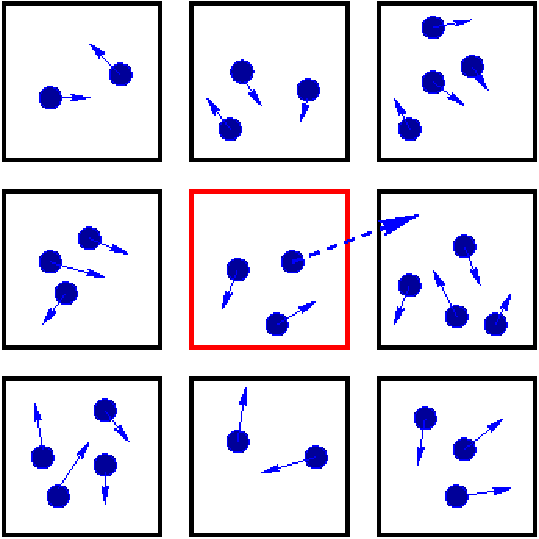
\includegraphics[width=0.7\textwidth]{figs/unit06_reservoir.pdf}
\end{center}

Although we draw a box around each replica (and colour one red to highlight the system \Om we will consider), these boxes are now merely mental constructions, and don't interfere with particles moving from one replica to another.
For example, we could take our system to be a cubic centimetre of air in a room, with the rest of the room forming its reservoir.
As in \secref{sec:replicas}, we assume that this system $\Om = \left\{\om_1, \om_2, \cdots, \om_M\right\}$ has a finite number of $M$ possible micro-states, where now different micro-states may involve different numbers of particles.

This again allows us to analyze the overall system of $R$ replicas in terms of occupation numbers $n_i$ and the corresponding occupation probabilities $p_i$.
Recall that $n_i$ is the number of replicas that adopt the micro-state $\om_i \in \Om$ in any given micro-state of the overall system $\Om_{\text{tot}}$, so that $\sum_i n_i = R$.
Similarly, $p_i = n_i / R$ is the probability that a randomly chosen replica will be in micro-state $\om_i$, with $\sum_i p_i = 1$ as usual.
In terms of $n_i$ and $p_i$, the total number of micro-states of $\Om_{\text{tot}}$, and the corresponding entropy, are the same as we derived in \secref{sec:canon_part},
\begin{equation*}
  M_{\text{tot}} = \frac{R!}{n_1! \; n_2! \; \cdots \; n_M!} \qquad \lra \qquad S(\Etot, \Ntot) = -R \sum_{i = 1}^M p_i \log p_i,
\end{equation*}
assuming $R \gg 1$ and $n_i \gg 1$ for all $i = 1, \cdots, M$.
In this expression, the dependence on both \Etot and \Ntot now enters through the occupation probabilities $p_i$, since the micro-states $\om_i$ may involve different numbers of particles in addition to different energies.

As before, we want to determine the (intensive) temperature and chemical potential of the micro-canonical system $\Om_{\text{tot}}$ through Eqs.~\ref{eq:temperature} and \ref{eq:chem_pot}, which requires expressing $S$ directly in terms of \Etot and $\Ntot$.
We again proceed by maximizing the entropy subject to the constraints on the conserved quantities of $\Om_{\text{tot}}$.
Labelling the energy and particle number of each replica $E_r$ and $N_r$, respectively, as in \eq{eq:canon_Etot} we can rearrange sums over replicas into sums over the micro-states of $\Om$:
\begin{align}
  1 & = \sum_{i = 1}^M p_i & \Etot = \sum_{r = 1}^R E_r = \sum_{i = 1}^M n_i E_i & = R \sum_{i = 1}^M p_i E_i \cr
    &                      & \Ntot = \sum_{r = 1}^R N_r = \sum_{i = 1}^M n_i N_i & = R \sum_{i = 1}^M p_i N_i, \label{eq:grand_constraint}
\end{align}
where $E_i$ and $N_i$ are the energies and particle numbers of the $M$ micro-states $\om_i \in \Om$.
The first two constraints, on the occupation probabilities and the total energy, are the same as we had in \secref{sec:canon_part}.
The third constraint, on the total particle number, is the new ingredient for us to incorporate.

Writing everything in terms of occupation probabilities, we see that we need to maximize the modified entropy
\begin{align*}
  \Sbar = -R \sum_{i = 1}^M p_i \log p_i & + \al\left(\sum_{i = 1}^M p_i - 1\right) \\
                                         & - \be\left(R \sum_{i = 1}^M p_i E_i - \Etot\right) + \ga\left(R \sum_{i = 1}^M p_i N_i - \Ntot\right),
\end{align*}
adding the Lagrange multiplier \ga to the \al and (negative) \be we previously had in \secref{sec:canon_part}.
What is the occupation probability $p_k$ that maximizes $\Sbar$?
\begin{mdframed}
  $\displaystyle 0 = \pderiv{\Sbar}{p_k} = $ \\[140 pt]
\end{mdframed}

You should find a probability of the form
\begin{equation}
  \label{eq:grand_Lagrange}
  p_k = \frac{1}{Z_g} e^{-\be E_k + \ga N_k},
\end{equation}
defining $Z_g = \exp\left[1 - \frac{\al}{R}\right]$ to work in terms of the parameters $\left\{Z_g, \be, \ga\right\}$.
As usual, we fix these three parameters by demanding that the three constraints above are satisfied.

\newpage % WARNING: FORMATTING BY HAND
Using the first constraint, what is $Z_g$ in terms of \be and $\ga$?
\begin{mdframed}
  $\displaystyle 1 = \sum_{i = 1}^M p_i = $ \\[50 pt]
\end{mdframed}

Analogously to \eq{eq:canon_aveE} in \secref{sec:canon_part}, the other two constraints
\begin{align*}
  \Etot & = R \sum_i p_i E_i &
  \Ntot & = R \sum_i p_i N_i
\end{align*}
now produce complicated relations between $\left\{\be, \ga\right\}$ and $\left\{\Etot, \Ntot\right\}$:
\begin{align}
  \Etot & = R \frac{\sum_{i = 1}^M E_i \; e^{-\be E_i + \ga N_i}}{\sum_{j = 1}^M e^{-\be E_j + \ga N_j}} = -\frac{R}{Z_g} \pderiv{}{\be} \sum_{i = 1}^M e^{-\be E_i + \ga N_i} = -R \pderiv{}{\be} \log Z_g(\be, \ga) \label{eq:grand_be_deriv} \\
  \Ntot & = R \frac{\sum_{i = 1}^M N_i \; e^{-\be E_i + \ga N_i}}{\sum_{j = 1}^M e^{-\be E_j + \ga N_j}} =  \frac{R}{Z_g} \pderiv{}{\ga} \sum_{i = 1}^M e^{-\be E_i + \ga N_i} =  R \pderiv{}{\ga} \log Z_g(\be, \ga). \label{eq:grand_ga_deriv}
\end{align}
These relations between $\left\{\Etot, \Ntot\right\}$ and partial derivatives of $\log Z_g$ will be useful when we consider the partial derivatives of the entropy that define the temperature and chemical potential.
Of course, in order to consider those partial derivatives, we need to express the entropy itself in terms of $\Etot$, \Ntot and the parameters
\begin{equation*}
  \left\{Z_g(\be, \ga), \qquad \be(\Etot, \Ntot), \qquad \ga(\Etot, \Ntot)\right\}
\end{equation*}
that we have now related to \Etot and $\Ntot$.
What do you obtain upon inserting \eq{eq:grand_Lagrange} for $p_i$ into the formula for the entropy?
\begin{mdframed}
  $\displaystyle S(\Etot, \Ntot) = -R \sum_{i = 1}^M p_i \log p_i = $ \\[120 pt]
\end{mdframed}

\newpage % WARNING: FORMATTING BY HAND
Taking the derivative of the resulting entropy with respect to $\Etot$, keeping \Ntot fixed, gives the temperature from \eq{eq:temperature}.
Thanks to Eqs.~\ref{eq:grand_be_deriv} and \ref{eq:grand_ga_deriv}, the result should simplify in a pleasant way:
\begin{mdframed}
  $\displaystyle \frac{1}{T} = \left. \pderiv{S}{\Etot}\right|_{\Ntot} = $ \\[100 pt]
\end{mdframed}
In the same way, the derivative with respect to $\Ntot$, keeping $\Etot$ fixed, gives the chemical potential with similar simplifications:
\begin{mdframed}
  $\displaystyle \mu = \left. -T \pderiv{S}{\Ntot}\right|_{\Etot} = $ \\[100 pt]
\end{mdframed}
In the end you should find
\begin{align}
  \be & = \frac{1}{T} &
  \ga & = \be \mu = \frac{\mu}{T},
\end{align}
meaning that (as desired) all information about the particle reservoir has dropped out, with no remaining reference to $R$, \Etot or $\Ntot$.
This large external reservoir is still present to fix the temperature $T$ and chemical potential $\mu$ that characterize the grand-canonical system $\Om$, but beyond that nothing about it is relevant (or even knowable) in the grand-canonical approach.

Every aspect of \Om can now be specified in terms of its fixed temperature $T$ and chemical potential $\mu$, starting with the parameters $\be = 1 / T$ and $\ga = \mu / T$.
In particular, the thermodynamic equilibrium probability that \Om adopts micro-state $\om_i$ with (non-conserved) internal energy $E_i$ and particle number $N_i$ is
\begin{equation}
  \label{eq:grand_prob}
  p_i = \frac{1}{Z_g} e^{-\be (E_i - \mu N_i)} = \frac{1}{Z_g} e^{-(E_i - \mu N_i) / T}.
\end{equation}
Since the particle number $N_i$ is dimensionless, the combination $E_i - \mu N_i$ that appears here reflects our observation below \eq{eq:chem_pot} that the chemical potential $\mu$ has dimensions of energy.

\begin{shaded}
  These micro-state probabilities are normalized by the \textbf{grand-canonical partition function}
  \begin{equation}
    \label{eq:grand_part_func}
    Z_g(T, \mu) = \sum_{i = 1}^M e^{-\be (E_i - \mu N_i)} = \sum_{i = 1}^M e^{-(E_i - \mu N_i) / T}.
  \end{equation}
  Analogously to the canonical partition function, this $Z_g$ is a fundamental quantity in the grand-canonical ensemble, from which many other derived quantities can be obtained.
\end{shaded}
% ------------------------------------------------------------------



% ------------------------------------------------------------------
\subsection{\label{sec:grand_pot}The grand-canonical potential, internal energy, entropy, and particle number}
The development of the grand-canonical ensemble we have seen so far closely resembles our earlier work setting up the canonical ensemble.
We have generalized the thermal reservoir to a particle reservoir that fixes both the temperature $T$ and chemical potential $\mu$, while allowing the system's internal energy and particle number to vary between different micro-states $\om_i$.
By adapting the replica ansatz to this setup, we determined the micro-state probabilities $p_i$ and the grand-canonical partition function $Z_g$, confirming that they are independent of the details of the particle reservoir.

We now continue by considering a similar set of derived quantities for the grand-canonical ensemble in thermodynamic equilibrium.
In addition to the expectation value of the internal energy introduced in \secref{sec:canon_derived}, the fluctuations of the particle number mean that we also need to consider its expectation value,
\begin{align*}
  \vev{E}\!(T, \mu) & = \sum_{i = 1}^M E_i \; p_i = \frac{1}{Z_g} \sum_{i = 1}^M E_i \; e^{-\be (E_i - \mu N_i)} \\
  \vev{N}\!(T, \mu) & = \sum_{i = 1}^M N_i \; p_i = \frac{1}{Z_g} \sum_{i = 1}^M N_i \; e^{-\be (E_i - \mu N_i)}.
\end{align*}
Looking back to Eqs.~\ref{eq:grand_be_deriv} and \ref{eq:grand_ga_deriv}, we can expect both of these derived quantities to be related to derivatives of the logarithm of the grand-canonical partition function.
In \secref{sec:Helmholtz}, similar relations led us to define the Helmholtz free energy for the canonical ensemble, which we can also generalize to the grand-canonical case.

\begin{shaded}
  We define the \textbf{grand-canonical potential} of a grand-canonical ensemble to be
  \begin{equation}
    \label{eq:grand_pot}
    \Phi(T, \mu) = -T \log Z_g(T, \mu) = -\frac{\log Z_g(\be, \mu)}{\be},
  \end{equation}
  where $Z_g$ is the grand-canonical partition function of the ensemble.
  In terms of this quantity, Eqs.~\ref{eq:grand_prob} and \ref{eq:grand_part_func} are
  \begin{align*}
    Z_g & = e^{-\Phi / T} &
    p_i & = e^{(\Phi - E_i + \mu N_i) / T}.
  \end{align*}
\end{shaded}

The grand-canonical potential is sometimes called the \textit{Landau free energy}, named after \href{https://en.wikipedia.org/wiki/Lev_Landau}{Lev Landau}, to highlight its similarity with the Helmholtz free energy.
As mentioned above, we want to consider derivatives of the grand-canonical potential, the simplest of which is with respect to the chemical potential,
\begin{mdframed}
  $\displaystyle \pderiv{}{\mu} \Phi(\be, \mu) = $ \\[120 pt]
\end{mdframed}
The derivative with respect to the temperature is a little messier, but can be simplified by recalling $\pderiv{}{T} = -\be^2 \pderiv{}{\be}$ from \eq{eq:beta_T}.
As in \secref{sec:Helmholtz}, it involves $\pderiv{}{T} \log Z_g$, which is again worth collecting in advance,
\begin{mdframed}
  $\displaystyle -\pderiv{}{T}\left[\frac{\Phi(T, \mu)}{T}\right] = \pderiv{}{T} \log Z_g(T, \mu) = $ \\[100 pt]
  $\displaystyle \pderiv{}{T} \Phi(T, \mu) = $ \\[80 pt]
\end{mdframed}
You should find
\begin{equation*}
  \pderiv{\Phi}{T} = \frac{\Phi - \vev{E} + \mu\vev{N}}{T} = -\log Z_g - \be\vev{E} + \be\mu\vev{N},
\end{equation*}
\newpage % WARNING: FORMATTING BY HAND
\noindent which we can connect to the entropy by inserting the probabilities $p_i$ from \eq{eq:grand_prob} into the general definition of the entropy from \eq{eq:entropy}:
\begin{mdframed}
  $\displaystyle S(T, \mu) = -\sum_{i = 1}^M p_i \log p_i = $ \\[100 pt]
\end{mdframed}

\begin{shaded}
  From this work we can read off the following relations involving the grand-canonical potential $\Phi(T, \mu)$:
  \begin{align}
    \vev{N}\!(T, \mu) & = -\pderiv{}{\mu} \Phi \label{eq:N_grand} \\
            S(T, \mu) & = -\pderiv{}{T} \Phi \\
    \vev{E}\!(T, \mu) & = -T^2 \pderiv{}{T} \left[\frac{\Phi}{T}\right] + \mu \vev{N} \label{eq:E_grand} \\
         \Phi(T, \mu) & = -T \, S + \vev{E} - \mu \vev{N} \label{eq:grand_relation}
  \end{align}
\end{shaded}

Finally, the connections between the energy, entropy and particle number provided by these relations motivate a further extension of the generalized first law of thermodynamics we derived in \eq{eq:first_law}.
To make the notation less cumbersome here, we write $\vev{E}$ and $\vev{N}$ as $E$ and $N$, keeping in mind that these are properties of the system's thermodynamic macro-state rather than its fluctuating micro-state.
In this notation, \eq{eq:first_law} reads $\d{E} = T \d{S} - P \d{V} = Q + W$, and relates any changes in the internal energy of a canonical system to changes in its entropy (heat) or volume (work).

Extending this to the grand-canonical ensemble, we can express the entropy as a function of the internal energy, volume and particle number, $S(E, V, N)$, and consider the change in entropy due to changes in each of these three parameters,
\begin{equation*}
  \d{S} = \left.\pderiv{S}{E}\right|_{V, N} \d{E} + \left.\pderiv{S}{V}\right|_{E, N} \d{V} + \left.\pderiv{S}{N}\right|_{V, E} \d{N} = \frac{1}{T} \d{E} + \left.\pderiv{S}{V}\right|_{E, N} \d{V} - \frac{\mu}{T} \d{N}.
\end{equation*}
We can interpret the remaining partial derivative by considering \eq{eq:first_law} in the case of fixed internal energy $E$.
This equation already incorporates the fixed particle number $N$, since it was derived in the framework of the canonical ensemble:
\begin{equation*}
  \d{E} = 0 = T \d{S} - P \d{V} \qquad \Lra \qquad \left.\pderiv{S}{V}\right|_{E, N} = \frac{P}{T}.
\end{equation*}

Putting things together, we obtain the generalized thermodynamic identity
\begin{equation}
  \label{eq:thermo_ident}
  \d{E} = T \d{S} - P \d{V} + \mu \d{N}.
\end{equation}
Due to this result, the term $\mu \d{N}$ is sometimes referred to as ``chemical work'', in analogy to the mechanical work $W = - P \d{V}$ done on a system by changing its volume.
This thermodynamic identity provides a convenient way to remember (or derive) relations between the internal energy, entropy, volume and particle number in thermodynamic equilibrium, by considering processes in which any two of these are fixed.
For example, fixing $N$ and $V$ gets us back to \eq{eq:temperature} for the temperature,
\begin{equation*}
  \d{E} = T \d{S} \qquad \Lra \qquad \frac{1}{T} = \left.\pderiv{S}{E}\right|_{N, V},
\end{equation*}
while fixing $N$ and $S$ gives \eq{eq:pressure} for the pressure,
\begin{equation*}
  \d{E} = -P \d{V} \qquad \Lra \qquad P = -\left.\pderiv{E}{V}\right|_{N, S}.
\end{equation*}

If we fix the entropy $S$ and volume $V$, we end up with another way of understanding the chemical potential,
\begin{equation}
  \label{eq:mu_E}
  \d{E} = \mu \d{N} \qquad \Lra \qquad \mu = \left.\pderiv{E}{N}\right|_{S, V}.
\end{equation}
That is, the chemical potential is the change in the internal energy when we change the number of particles in the system, without changing its entropy or volume.
If we consider adding particles to the system, $\De N > 0$, we argued below \eq{eq:chem_pot} that we should generically expect an increase in the entropy.
In order to keep the entropy fixed in this process, we therefore need the change in the energy to decrease the entropy by the corresponding amount.
For natural systems with positive temperatures, this requires decreasing the energy, $\De E < 0$.
Similarly, keeping the entropy fixed as we decrease $N$ would require increasing $E$, so that \eq{eq:mu_E} confirms our earlier finding that for natural systems the chemical potential is negative in general.
% ------------------------------------------------------------------


\newpage
% ------------------------------------------------------------------
\renewcommand{\thisunit}{MATH327 Unit 7}
\renewcommand{\moddate}{Last modified 17 Mar.~2025}
\setcounter{section}{7}
\setcounter{subsection}{0}
\phantomsection
\addcontentsline{toc}{section}{Unit 7: Quantum statistics}
\section*{Unit 7: Quantum statistics}
\subsection{\label{sec:quantum}Quantized energy levels and their micro-states}
Now that we have defined the grand-canonical ensemble, we will apply it to investigate quantum statistical systems.
The first step is to introduce quantum statistics itself --- it is worth reiterating that no prior knowledge of quantum physics is assumed, nor will this module attempt to teach quantum mechanics.
We will simply consider quantum behaviour as an ansatz (that turns out to be realized in nature), and analyse the resulting systems by making use of the statistical mechanics tools we have developed.

Quantum physics was mentioned in passing during our derivation of the canonical partition function for a classical (non-quantum) ideal gas in \secref{sec:regulate}.
You may have felt that this derivation involved seemingly circular reasoning.
First, because the partition function is defined as a sum over micro-states $\om_i$,
\begin{equation*}
  Z = \sum_i e^{-E(\vec{p}_i) / T},
\end{equation*}
we regularized the system by supposing that the gas particles' momenta $\vec{p}_i$ are \textit{quantized} and can take only particular discrete values, rather than varying continuously.
These quantized momenta produce a countable number of discrete \textit{energy levels}, leading to a countable number of micro-states and hence a well-defined partition function that involves sums over all possible discrete momenta for each particle.
Second, after the system was regularized, we switched back to continuously varying momenta, converting sums to integrals while retaining the dimensionful factors we had derived along the way.

Two changes are required to define quantum statistics.
First, not surprisingly, we need to retain discrete energy levels rather than approximating these as continuous.
This will allow our calculations to remain valid even in the quantum regime where $L\sqrt{mT} \sim \hbar$ (or equivalently $\lath^3 \sim V$).
The second change is more subtle, and is connected to the fundamental indistinguishability of identical particles governed by quantum mechanics --- a fact about nature that we will take as given.
The issue is how to handle micro-states in which multiple indistinguishable particles occupy the same energy level.

To build up to this issue, we will first see what happens when we ignore it and apply our usual classical approach to compute the grand-canonical partition function for a system with discrete energy levels.
Despite the quantized energy levels, this calculation will still produce a non-quantum result known as \textbf{Maxwell--Boltzmann} (MB) statistics, named after \href{https://en.wikipedia.org/wiki/James_Clerk_Maxwell}{James Clerk Maxwell} and Ludwig Boltzmann.
We will then consider how this approach can break down, and use this insight to develop true quantum statistics in the following sections.
Finally, we will wrap up this unit by confirming that Maxwell--Boltzmann statistics remains an excellent approximation to quantum statistics in the classical limit.
% ------------------------------------------------------------------



% ------------------------------------------------------------------
\subsubsection{Maxwell--Boltzmann statistics}
Let's begin our classical derivation of the grand-canonical partition function for a system with discrete energy levels by defining some necessary notation.
We label the discrete energy levels $\cE_{\ell}$ for $\ell = 0$, $1$, $\cdots$, $\cL$, where $\cL$ can be taken to infinity while retaining a countable number of micro-states and hence well-defined partition functions.
The energy level $\cE_{\ell}$ may be characterized by extra information in addition to the actual value of its energy, $E_{\ell}$.
As we saw in \secref{sec:regulate}, it is therefore possible for distinct energy levels $\left\{\cE_m, \cE_n\right\}$ to have the same energy $E_m = E_n$ for $m \neq n$. % TODO: This was for permutations of momentum components.  Another example could be different locations...
Such energy levels with the same value of the energy are said to be \textit{degenerate}.
We will label energy levels so that $E_m \leq E_n$ for $m < n$.
Without loss of generality, we can take $E_{\ell} \geq E_0 \geq 0$.

Now starting from the general expression for the grand-canonical partition function, \eq{eq:grand_part_func},
\begin{equation*}
  Z_g(\be, \mu) = \sum_i e^{-\be (E_i - \mu N_i)},
\end{equation*}
we just need to define the micro-states $\om_i$ with energy $E_i$ and particle number $N_i$.
In the classical Maxwell--Boltzmann approach, we arrange this into a series of sums with fixed particle numbers:
\begin{equation*}
  \ZMB(\be, \mu) = \sum_{i, N_i = 0} e^{-\be E_i} + \sum_{j, N_j = 1} e^{-\be (E_j - \mu)} + \sum_{k, N_k = 2} e^{-\be (E_k - 2\mu)} + \cdots,
\end{equation*}
where the micro-states labelled $\left\{\om_i, \om_j, \om_k, \cdots\right\}$ are those that have $N = 0$, $1$, $2$, $\cdots$ particles, respectively.
We can recognize $N$-particle canonical partition functions $Z_N(\be)$ in the expression above:
\begin{equation}
  \label{eq:fugacity_exp}
  \ZMB(\be, \mu) = Z_0(\be) + e^{\be\mu} Z_1(\be) + e^{2\be\mu} Z_2(\be) + \cdots = \sum_{N = 0}^{\infty} \left[e^{\be\mu}\right]^N Z_N(\be).
\end{equation}
This is a general result known as the \textit{fugacity expansion}, where $e^{\be\mu}$ is called the fugacity.
Organizing the calculation in this way allows us to take advantage of our experience with the canonical ensemble.

In particular, because we continue to consider only `ideal' systems in which the particles don't interact with each other, each $Z_N(\be)$ is simply the product of the single-particle partition functions $Z_1(\be)$ for all $N$ independent particles,
\begin{equation*}
  Z_N(\be) = \frac{1}{N!} \left[Z_1(\be)\right]^N,
\end{equation*}
with the factor of $N!$ included to correct for over-counting indistinguishable particles.
This is exactly the derivation we performed in \secref{sec:regulate}, to obtain \eq{eq:ideal_indis} for the classical ideal gas.
Inserting this $Z_N$ into \eq{eq:fugacity_exp}, we have
\begin{equation*}
  \ZMB(\be, \mu) = \sum_{N = 0}^{\infty} \left[e^{\be\mu}\right]^N \frac{1}{N!} \left[Z_1(\be)\right]^N = \sum_{N = 0}^{\infty} \frac{1}{N!} \left[e^{\be\mu} Z_1(\be)\right]^N = \exp\left[e^{\be\mu} Z_1(\be)\right].
\end{equation*}
In the case of a system with discrete energy levels $\cE_{\ell}$, the single-particle partition function is simply
\begin{equation*}
  Z_1(\be) = \sum_{\ell = 0}^{\cL} e^{-\be E_{\ell}},
\end{equation*}
where each micro-state has the particle in a different energy level.
This gives us the Maxwell--Boltzmann grand-canonical partition function
\begin{equation}
  \label{eq:partfunc_MB_nonfactor}
  \ZMB(\be, \mu) = \exp\left[e^{\be\mu} \sum_{\ell = 0}^{\cL} e^{-\be E_{\ell}} \right] = \exp\left[\sum_{\ell = 0}^{\cL} e^{-\be\left(E_{\ell} - \mu\right)}\right].
\end{equation}
% ------------------------------------------------------------------



% ------------------------------------------------------------------
\subsubsection{Over-counting and quantum statistics}
The problem with the derivation above was already mentioned in the footnote accompanying \eq{eq:ideal_indis}.
Recall that the factor of $\frac{1}{N!}$ comes from the $N!$ different ways the $N$ particles could be labeled --- since indistinguishable particles cannot be labeled, we have only a single micro-state rather than the $N!$ micro-states arising from $Z_1^N$ itself.
We will see that this analysis is only correct when each of the particles is in a different energy level.
When the particles' energies can vary continuously it is practically impossible for two of them to have exactly the same energy, making it safe to assume a different energy level for each particle.
More generally, this assumption can remain an excellent approximation whenever there are many more accessible energy levels than there are particles to occupy them.
Here we are interested in situations where there is a non-negligible chance of multiple particles occupying the same energy level, which we can call the `quantum regime').

Let's illustrate the problem by considering a simple system with $N = 2$ particles that can each occupy any of five energy levels, $\cE_0$ through $\cE_4$.
The canonical partition function for this system sums over all possible ways these particles can occupy the available energy levels --- equivalent to the ways $N = 2$ balls can be placed into $\cL + 1 = 5$ boxes.
We can represent possible micro-states by drawing these balls and boxes, for example $\boxzero\boxone\boxzero\boxzero\boxone$ and $\boxzero\boxzero\boxtwo\boxzero\boxzero$.
How many terms are there in the sum for the distinguishable partition function, $Z_D$?
\begin{mdframed}
  \ \\[24 pt]
\end{mdframed}
For indistinguishable particles, our earlier derivation predicts there are half as many ($\frac{1}{2!}$) terms in the sum for the indistinguishable partition function, $Z_I$, but this would be a non-integer number of terms and therefore cannot be correct.

We can see where the derivation goes wrong by explicitly writing down all the micro-states in both cases of distinguishable and indistinguishable particles.
In the distinguishable case, we can suppose that the balls are red ($\textcolor{red}{\bullet}$) and blue ($\textcolor{blue}{\bullet}$), and compactly represent micro-states by recording whether each box is empty (``$0$'') or contains the red ball (``$R$''), the blue ball (``$B$'') or both balls (``$2$''):
\begin{align*}
  \boxzero\boxzero\boxed{\textcolor{red}{\bullet}}\boxzero\boxed{\textcolor{blue}{\bullet}} & = 00R0B &
  \boxzero\boxzero\boxed{\textcolor{red}{\bullet}\textcolor{blue}{\bullet}}\boxzero\boxzero & = 00200.
\end{align*}
The full set of micro-states is then
\begin{align*}
  RB000 & & 0R0B0 & & BR000 & & 0B0R0 & & 20000 \\
  R0B00 & & 0R00B & & B0R00 & & 0B00R & & 02000 \\
  R00B0 & & 00RB0 & & B00R0 & & 00BR0 & & 00200 \\
  R000B & & 00R0B & & B000R & & 00B0R & & 00020 \\
  0RB00 & & 000RB & & 0BR00 & & 000BR & & 00002
\end{align*}

If we now consider indistinguishable particles where we can only know the number of particles in each box ($R, B \to 1$), we see that the third and fourth columns above duplicate the first two columns.
This is exactly the over-counting that the usual factor of $\frac{1}{N!} = \frac{1}{2}$ corrects.
On the other hand, the micro-states in the final column, with both particles in the same energy level, were not over-counted, and must not be divided by $N!$.
This leaves us with $15$ micro-states, rather than $25/2$:
\begin{align*}
  11000 & & 01010 & & 20000 \\
  10100 & & 01001 & & 02000 \\
  10010 & & 00110 & & 00200 \\
  10001 & & 00101 & & 00020 \\
  01100 & & 00011 & & 00002
\end{align*}

We can generalize this simple exercise by systematically labeling the micro-states for indistinguishable particles by \textit{occupation numbers} $n_{\ell}$, similar to those that we encountered when using replicas to set up the canonical ensemble in \secref{sec:reservoir} and the grand-canonical ensemble in \secref{sec:Zg}.
In this case the occupation number $n_{\ell}$ is simply the number of particles in energy level $\cE_{\ell}$.
This new approach is the second change promised above, and the final ingredient needed for the following definition.

\begin{shaded}
  In \textbf{quantum statistics}, the micro-states are defined by considering each energy level $\cE_{\ell}$ in turn, and summing over the possible occupation numbers $n_{\ell}$ that it could have.
  This differs from the classical approach in which the micro-states were defined by considering each particle in turn, and summing over the possible energies (etc.) that it could have.
\end{shaded}

Because quantum mechanics requires all particles of the same type to be indistinguishable, the classical approach forces us to correct for over-counting, and we have now seen how this becomes non-trivial whenever multiple particles can occupy the same energy level.
The quantum approach of summing over the occupation numbers of the quantized energy levels avoids this issue, and doesn't encounter any over-counting that would require correction.
% ------------------------------------------------------------------



% ------------------------------------------------------------------
\subsection{\label{sec:spin}Bosons and fermions}
In Sections~\ref{sec:bose} and \ref{sec:fermi} we will carry out explicit computations to show how the quantum statistics defined above work in practice.
In preparation, we will take into account some additional information about nature, specifically concerning the occupation numbers $n_{\ell}$ that are possible for each energy level $\cE_{\ell}$.
As before, for the purposes of this module we can simply consider this information to be part of our ansatz.

Using quantum mechanics and special relativity, it is possible to prove that all particles in three spatial dimensions fall into two distinct classes.
(\href{https://en.wikipedia.org/wiki/Anyon}{More exotic behaviour} is possible for particles confined to two-dimensional surfaces.)
This result is known as the \href{https://en.wikipedia.org/wiki/Spin-statistics_theorem}{spin--statistics theorem}, while the two types of particles it describes are called \textbf{bosons} (named after \href{https://en.wikipedia.org/wiki/Satyendra_Nath_Bose}{Satyendra Nath Bose}) and \textbf{fermions} (named after \href{https://en.wikipedia.org/wiki/Enrico_Fermi}{Enrico Fermi}).
These two classes of particles obey different rules for their possible occupation numbers, and therefore give rise to distinct quantum statistics.

Any non-negative number of identical bosons can simultaneously occupy the same energy level, corresponding to occupation numbers $n_{\ell} = 0$, $1$, $2$, $\cdots$.
Physical examples of bosons include photons (particles of light), pions, helium-$4$ atoms and the famous Higgs particle.

In contrast, it is impossible for multiple identical fermions to occupy the same energy level, meaning that their only possible occupation numbers are $n_{\ell} = 0$ and $1$.
This behaviour is known as the \textit{Pauli exclusion principle} (named after \href{https://en.wikipedia.org/wiki/Wolfgang_Pauli}{Wolfgang Pauli}) and has extremely important consequences, including the existence of chemistry and life.
Physical examples of fermions include electrons, protons, neutrons, neutrinos and helium-$3$ atoms.

The reason multiple identical fermions cannot occupy the same energy level is due to a feature of quantum mechanics, and not because they physically repel each other.
This paragraph will imprecisely describe how this works, for those who may be curious, and can be skipped without any problem.
Consider a system of identical quantum particles occupying various energy levels.
Loosely speaking, all observable properties of this system depend on the \emph{square} of the quantum function that defines it.
Interchanging any pair of indistinguishable particles must leave all these observable properties unchanged.
Just as $\sqrt{1} = \pm 1$, there are two ways the underlying quantum function can behave to leave its square unchanged: it can be completely symmetric or completely antisymmetric under all possible interchanges.
Bosons correspond to the symmetric case, while fermions correspond to the antisymmetric case.
At the same time, if two identical particles occupy the same energy level, then the quantum function itself is unchanged (i.e., symmetric) when they are interchanged.
In the fermionic case, the resulting quantum function must therefore be simultaneously symmetric and antisymmetric, which is only possible if it is exactly zero.
In other words no systems with multiple identical fermions in the same energy level can possibly exist.

Looking back at the example system of $N = 2$ particles with five energy levels in the previous section, all $15$ micro-states we wrote down are possible if the particles are bosons.
How many micro-states are allowed if the particles are fermions?
\begin{mdframed}
  \ \\[15 pt]
\end{mdframed}
This difference in the possible micro-states ensures that bosons and fermions exhibit different quantum statistics.
We will now consider each case in turn.
% ------------------------------------------------------------------



% ------------------------------------------------------------------
\subsection{\label{sec:bose}Bose--Einstein statistics}
The quantum statistics of bosons is known as \textbf{Bose--Einstein} (BE) statistics, named after Satyendra Nath Bose and Albert Einstein.
As described above, to carry out the sum over all micro-states in the grand-canonical partition function
\begin{equation*}
  Z_g(\be, \mu) = \sum_i e^{-\be (E_i - \mu N_i)},
\end{equation*}
we first sum over all energy levels $\cE_{\ell}$, and then over all possible occupation numbers $n_{\ell} \in \Nbb_0$ for each energy level.

Consider first the simple case of a system that only has a single energy level $\cE_0$, with energy $E_0$.
In this case, each micro-state $\om_i$ is uniquely described by its particle number $N_i$, which is just the occupation number of $\cE_0$.
What is the energy $E_i$ of micro-state $\om_i$ with occupation number $n_0 = N_i$?
\begin{mdframed}
  $E_i = $ \\[24 pt]
\end{mdframed}
Summing over all possible occupation numbers for this single energy level, the Bose--Einstein grand-canonical partition function for this system is
\begin{equation}
  \label{eq:BEsingle}
  \ZBE(\be, \mu) = \sum_{n_0 = 0}^{\infty} e^{-\be (E_0 - \mu) n_0} = \sum_{n_0 = 0}^{\infty} \left[e^{-\be (E_0 - \mu)}\right]^{n_0} = \frac{1}{1 - e^{-\be (E_0 - \mu)}}.
\end{equation}
In the last step we recognized the geometric series
\begin{equation*}
  \frac{1}{1 - x} = 1 + x + x^2 + \cdots,
\end{equation*}
which only converges for $x = e^{-\be (E_0 - \mu)} < 1$.
For natural systems with $\be = 1 / T > 0$, this condition requires $E_0 - \mu > 0$ or equivalently $\mu < E_0$.
Since we can take all $E_{\ell} \geq 0$ without loss of generality, this constraint is consistent with the negative chemical potential $\mu < 0$ that we discussed in Unit~6.

At this point, it is straightforward to generalize to multiple energy levels $\cE_{\ell}$ with $\ell = 0$, $1$, $\cdots$, $\cL$.
For systems of non-interacting particles, the micro-state $\om_i$ defined by the set of occupation numbers $\left\{n_{\ell}\right\}$ has energy and particle number
\begin{align}
  \label{eq:total_energy_levels}
  E_i & = \sum_{\ell = 0}^{\cL} E_{\ell} \, n_{\ell} &
  N_i & = \sum_{\ell = 0}^{\cL} n_{\ell}.
\end{align}
The general Bose--Einstein grand-canonical partition function is therefore
\begin{equation*}
  \ZBE(\be, \mu) = \sum_{n_0 = 0}^{\infty} \sum_{n_1 = 0}^{\infty} \cdots \sum_{n_{\cL} = 0}^{\infty} \exp\left[-\be\sum_{\ell = 0}^{\cL} \left(E_{\ell} - \mu\right) n_{\ell}\right].
\end{equation*}
We can apply the identity $e^{\sum_i x_i} = \prod_i e^{x_i}$ to rewrite
\begin{equation*}
  \exp\left[-\be\sum_{\ell = 0}^{\cL} \left(E_{\ell} - \mu\right) n_{\ell}\right] = \left(e^{-\be (E_0 - \mu) n_0}\right) \left(e^{-\be (E_1 - \mu) n_1}\right)\cdots \left(e^{-\be (E_L - \mu) n_L}\right).
\end{equation*}
Recalling $\mu < E_{\ell}$ for all $\ell$, by rearranging the terms we find
\begin{align}
  \ZBE(\be, \mu) & = \left(\sum_{n_0 = 0}^{\infty} e^{-\be (E_0 - \mu) n_0}\right) \left(\sum_{n_1 = 0}^{\infty} e^{-\be (E_1 - \mu) n_1}\right)\cdots \left(\sum_{n_{\cL} = 0}^{\infty} e^{-\be (E_{\cL} - \mu) n_{\cL}}\right) \cr
                 & = \prod_{\ell = 0}^{\cL} \frac{1}{1 - e^{-\be (E_{\ell} - \mu)}}. \label{eq:partfunc_BE}
\end{align}

This grand-canonical partition function defines the quantum Bose--Einstein statistics of bosons.
Its structure as the product of an independent contribution for each energy level is reminiscent of the result $Z_N \propto Z_1^N$ for the classical $N$-particle canonical partition function discussed above.
In such situations we say that the calculation \textit{factorizes} into a product of many simpler terms, allowing us to build up the full result on the basis of much easier computations.
Looking back to \eq{eq:partfunc_MB_nonfactor}, we can also observe factorization in the classical Maxwell--Boltzmann grand-canonical partition function,
\begin{equation}
  \label{eq:partfunc_MB}
  \ZMB(\be, \mu) = \exp\left[\sum_{\ell = 0}^{\cL} e^{-\be\left(E_{\ell} - \mu\right)}\right] = \prod_{\ell = 0}^{\cL} \exp\left[e^{-\be\left(E_{\ell} - \mu\right)}\right].
\end{equation}
In both cases factorization results from working with non-interacting particles.
Starting in Unit~9 we will consider non-ideal systems in which the particles can interact with each other, where the absence of factorization will make analyses much more difficult.
% ------------------------------------------------------------------



% ------------------------------------------------------------------
\subsection{\label{sec:fermi}Fermi--Dirac statistics}
Next, the quantum statistics of fermions is known as \textbf{Fermi--Dirac} (FD) statistics, named after Enrico Fermi and \href{https://en.wikipedia.org/wiki/Paul_Dirac}{Paul Dirac}.
The derivation of the Fermi--Dirac grand-canonical partition function is very similar to the Bose--Einstein case above.
We again proceed by summing over all energy levels $\cE_{\ell}$, and just have to account for the more limited possible occupation numbers $n_{\ell} \in \left\{0, 1\right\}$ for each energy level.

Taking the same approach of first considering a simple system with only a single energy level, \eq{eq:BEsingle} would just change to
\begin{equation*}
  \ZFD(\be, \mu) = \sum_{n_0 = 0}^1 e^{-\be (E_0 - \mu) n_0} = 1 + e^{-\be (E_0 - \mu)}.
\end{equation*}
Generalizing to multiple energy levels $\cE_{\ell}$ with $\ell = 0$, $1$, $\cdots$, $\cL$, the micro-state energies $E_i = \sum_{\ell} E_{\ell} \, n_{\ell}$ and particle numbers $N_i = \sum_{\ell} n_{\ell}$ remain the same as in \eq{eq:total_energy_levels}, and the computation again factorizes,
\begin{align}
  \ZFD(\be, \mu) & = \sum_{n_0 = 0}^1 \sum_{n_1 = 0}^1 \cdots \sum_{n_{\cL} = 0}^1 \exp\left[-\be\sum_{\ell = 0}^{\cL} \left(E_{\ell} - \mu\right) n_{\ell}\right] \cr
                 & = \left(\sum_{n_0 = 0}^1 e^{-\be (E_0 - \mu) n_0}\right) \left(\sum_{n_1 = 0}^1 e^{-\be (E_1 - \mu) n_1}\right)\cdots \left(\sum_{n_{\cL} = 0}^1 e^{-\be (E_{\cL} - \mu) n_{\cL}}\right) \cr
                 & = \prod_{\ell = 0}^{\cL} \left[1 + e^{-\be (E_{\ell} - \mu)}\right]. \label{eq:partfunc_FD}
\end{align}
This grand-canonical partition function defines the quantum Fermi--Dirac statistics of fermions.
In both this case and the case of classical Maxwell--Boltzmann statistics there is no constraint on $\be (E_{\ell} - \mu)$.

In Unit~8 we will take \ZBE and \ZFD as starting points to analyse quantum gases of bosons and fermions, respectively.
Before beginning those more detailed analyses, let's quickly compare the three types of statistics that we have derived in this unit, while they are all close to hand.
% ------------------------------------------------------------------



% ------------------------------------------------------------------
\subsection{\label{sec:quantum_classical}The classical limit}
In \secref{sec:quantum} we claimed that if the probability of multiple particles occupying the same energy level is negligible, then the classical Maxwell--Boltzmann statistics can be an excellent approximation to quantum statistics --- both bosonic and fermionic.
We will wrap up this unit by demonstrating this result and clarifying the conditions that correspond to this `classical limit' of quantum statistics.

It is useful to start by asking when we should expect classical statistics to predict a non-negligible probability for multiple particles to occupy the same energy level, leading to the over-counting problems that are solved by quantum statistics.
This is actually a question we have already considered, back in \secref{sec:spin_info}.
There we used the canonical ensemble to analyse classical spin systems with discrete energy levels, finding that at low temperatures the systems are dominated by their lowest-energy micro-states, with only exponentially suppressed corrections coming from any higher-energy micro-states.
In the present context, this corresponds to a classical prediction of exponentially small probabilities for particles to occupy any energy levels with $E_{\ell} > E_0$ --- effectively guaranteeing that the lowest energy level $\cE_0$ will be occupied by multiple particles and classical statistics will break down.

In short, the low-temperature regime is where quantum and classical statistics disagree, while \textbf{high temperatures correspond to the classical limit} of quantum statistics.
If you are not convinced by the argument leading to this conclusion, you can find a more detailed derivation based on the equation of state and thermal de~Broglie wavelength in Section~3.5 of David Tong's \href{https://www.damtp.cam.ac.uk/user/tong/statphys.html}{\textit{Lectures on Statistical Physics}}.

For now, we want to consider the grand-canonical ensemble at high temperatures, to see whether the quantum and classical statistics we derived in the previous sections become equivalent in this regime.
However, it can be subtle to work with the grand-canonical ensemble at high temperatures, due to the dependence of the average number of particles on the temperature.
To demonstrate this subtlety, let's compute the average particle number $\vev{N}\!(T, \mu)$ starting from the grand-canonical partition function, for both classical and quantum statistics.

For convenience, let's collect our earlier results for the grand-canonical partition functions corresponding to classical Maxwell--Boltzmann statistics (\eq{eq:partfunc_MB}), the quantum Bose--Einstein statistics of bosons (\eq{eq:partfunc_BE}) and the quantum Fermi--Dirac statistics of fermions (\eq{eq:partfunc_FD}):
\begin{equation*}
  \ZMB = \prod_{\ell = 0}^{\cL} \exp\left[e^{-\be\left(E_{\ell} - \mu\right)}\right]
\end{equation*}
\begin{align*}
  \ZBE & = \prod_{\ell = 0}^{\cL} \frac{1}{1 - e^{-\be (E_{\ell} - \mu)}} &
  \ZFD & = \prod_{\ell = 0}^{\cL} \left[1 + e^{-\be (E_{\ell} - \mu)}\right].
\end{align*}
Recalling $\log\left[\prod_i x_i\right] = \sum_i \log x_i$, the three corresponding grand-canonical potentials $\Phi = -T \log Z_g$ are
\begin{equation*}
  \Phi_{\text{MB}} = -T \sum_{\ell = 0}^{\cL} e^{-\be\left(E_{\ell} - \mu\right)}
\end{equation*}
\begin{align*}
  \Phi_{\text{BE}} & =  T \sum_{\ell = 0}^{\cL} \log\left[1 - e^{-\be (E_{\ell} - \mu)}\right] &
  \Phi_{\text{FD}} & = -T \sum_{\ell = 0}^{\cL} \log\left[1 + e^{-\be (E_{\ell} - \mu)}\right].
\end{align*}

We are now ready to compute the average particle numbers.
Using the result we derived in \secref{sec:grand_pot},
\begin{equation*}
  \vev{N} = -\pderiv{\Phi}{\mu},
\end{equation*}
what are the average particle numbers resulting from the three grand-canonical potentials above?
\begin{mdframed}
  $\displaystyle \vev{N}_{\text{MB}} = $ \\[52 pt]
  $\displaystyle \vev{N}_{\text{BE}} = $ \\[52 pt]
  $\displaystyle \vev{N}_{\text{FD}} = $ \\[52 pt]
\end{mdframed}

You should find that the average particle number in all three cases can be expressed as a sum over the average occupation numbers,
\begin{equation*}
  \vev{N} = \sum_{\ell = 0}^{\cL} \vev{n_{\ell}},
\end{equation*}
where the corresponding average occupation numbers are
\begin{equation*}
  \nMB = \frac{1}{e^{\be (E_{\ell} - \mu)}}
\end{equation*}
\begin{align*}
  \nBE & = \frac{1}{e^{\be (E_{\ell} - \mu)} - 1} &
  \nFD & = \frac{1}{e^{\be (E_{\ell} - \mu)} + 1}.
\end{align*}
Note that $\vev{n_{\ell}} \geq 0$ in all cases, and also $\nFD \leq 1$, as required for fermions.
From these results we see that the classical limit $\nBE \approx \nFD \approx \nMB$ corresponds to
\begin{equation*}
  e^{\be (E_{\ell} - \mu)} \pm 1 \approx e^{\be (E_{\ell} - \mu)} \qquad \Lra \qquad e^{\be (E_{\ell} - \mu)} \gg 1.
\end{equation*}
We can also confirm that this limit corresponds to $\vev{n_{\ell}} \ll 1$ for all energy levels $\cE_{\ell}$ and all three types of statistics, confirming our starting point of very small probabilities for multiple particles to occupy the same energy level.

Now we can appreciate the subtlety promised above, because
\begin{equation}
  \label{eq:highT_ratio}
  \be (E_{\ell} - \mu) = \frac{E_{\ell} - \mu}{T} \gg 1.
\end{equation}
does not look like a high-temperature limit!
Indeed, if we consider the naive high-temperature limit $\be = 1 / T \to 0$ with fixed $(E_{\ell} - \mu)$, we would find large average occupation numbers,
\begin{align*}
  \nMB & \approx 1 &
  \nBE & \to \infty & 
  \nFD & \approx \frac{1}{2}.
\end{align*}
In addition to implying non-negligible probabilities for multiple particles to occupy the same energy level, this result indicates that higher temperatures in the grand-canonical ensemble lead to larger particle numbers in total --- at least when $(E_{\ell} - \mu)$ is fixed. % Could note smaller mu/T implies less entropy response to change in particle number...

In order to balance this effect, we need to adjust the other parameter offered by the grand-canonical ensemble: the chemical potential $\mu$.
Specifically, in order to satisfy \eq{eq:highT_ratio} in the high-temperature limit, we need $E_{\ell} - \mu \gg T$, which requires that $\mu \to -\infty$ as $T \to \infty$.
Making the chemical potential more negative reduces the probability of having large numbers of particles in the system, at the same time as the smaller \be increases the number of energy levels that these particles can occupy with non-negligible probability.
Taken together, these two effects guarantee that there are many more accessible energy levels than there are particles, allowing us to conclude that the true high-temperature limit in which quantum statistics becomes classical is
\begin{equation}
  -\mu \gg T \gg E_{\ell} \qquad \Lra \qquad \frac{E_{\ell} - \mu}{T} \gg 1.
\end{equation}
This corresponds to the right edge of the plot on the next page, where we can confirm that all three sets of statistics predict essentially the same average occupation number $\vev{n_{\ell}}$ for any energy level $\cE_{\ell}$.

\begin{center}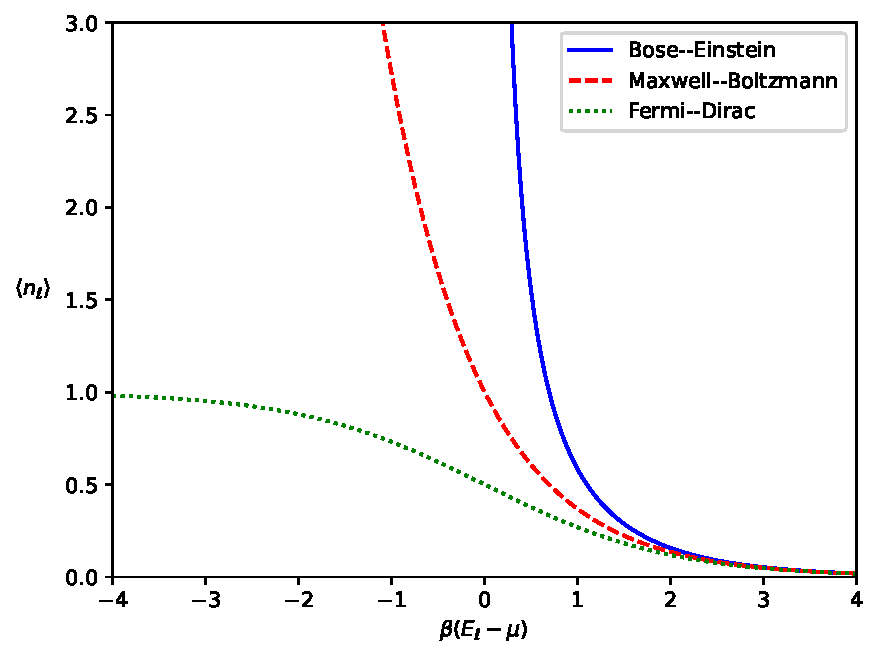
\includegraphics[width=\textwidth]{figs/unit07_dist.pdf}\end{center}

In the low-temperature regime $\frac{E_{\ell} - \mu}{T} \ll 1$ corresponding to the left portion of the plot, we see dramatically different behaviour for the three cases.
The classical Maxwell--Boltzmann prediction for the average occupation number grows exponentially, while the quantum Bose--Einstein prediction diverges as either $E_{\ell} \to \mu$ or $\be \to 0$ with $(E_{\ell} - \mu)$ fixed, and the Fermi--Dirac prediction slowly approaches its maximum possible value $\nFD \to 1$.
In the next unit we will explore these results in more detail by considering specific examples of quantum gases of bosons and fermions.
% ------------------------------------------------------------------


\newpage
% ------------------------------------------------------------------
\renewcommand{\thisunit}{MATH327 Unit 8}
\renewcommand{\moddate}{Last modified 2 Apr.~2025}
\setcounter{section}{8}
\setcounter{subsection}{0}
\phantomsection
\addcontentsline{toc}{section}{Unit 8: Quantum gases}
\section*{Unit 8: Quantum gases}
\subsection{\label{sec:photon}The photon gas}
\subsubsection{Massive bosons in a box}
In \secref{sec:bose} we derived the grand-canonical partition function (\eq{eq:partfunc_BE}) that defines quantum Bose--Einstein statistics for systems of non-interacting bosons,
\begin{equation*}
  \ZBE(\be, \mu) = \prod_{\ell = 0}^{\cL} \frac{1}{1 - e^{-\be (E_{\ell} - \mu)}}.
\end{equation*}
Following the quantum approach, we obtained this result by considering in turn each energy level $\cE_{\ell}$ with energy $E_{\ell}$, and summing over all possible occupation numbers that it could have.
For bosons, $n_{\ell} \in \Nbb_0$ produces sums that only converge if $\mu < E_{\ell}$ for all $\ell$.
The corresponding grand-canonical potential is
\begin{equation*}
  \Phi_{\text{BE}} = -T \log \ZBE = T \sum_{\ell = 0}^{\cL} \log\left[1 - e^{-\be (E_{\ell} - \mu)}\right],
\end{equation*}
from which we can determine the large-scale properties of the system, including its average internal energy $\vev{E}$, average particle number $\vev{N}$, entropy $S$, and pressure $P$.

To do so, we have to specify the energy levels of the particles that compose the system of interest, including any degenerate energy levels $\left\{\cE_m, \cE_n\right\}$ with the same energy $E_m = E_n$ for $m \neq n$.
One example of this that we have already considered is the analysis of non-relativistic ideal gas particles in \secref{sec:regulate}.
For a single particle with mass $m$ in a volume $V = L^3$, we adopted an ansatz for the quantized energies,
\begin{align}
  \label{eq:nonrel_energy}
  E(k_x, k_y, k_z) & = \frac{\hbar^2 \pi^2}{2mL^2}\left(k_x^2 + k_y^2 + k_z^2\right) = \eps k^2 \qquad &
  \eps & \equiv \frac{\hbar^2 \pi^2}{2mL^2},
\end{align}
where the positive integers $k_{x, y, z} = 1, 2, \cdots$ specify the possible momentum magnitude of the particle, $p = \hbar \frac{\pi}{L} k$.

Compared to \secref{sec:regulate}, where $k_{x, y, z} = 0$ was allowed, here we have adjusted our ansatz to require strictly positive values.
This adjustment is required by another feature of quantum mechanics, which this paragraph will imprecisely describe for the curious.
This description can be skipped without any problem, with the adjusted ansatz simply taken as input.
The feature at play here is known as \href{https://en.wikipedia.org/wiki/Uncertainty_principle}{Heisenberg's uncertainty principle} (named after \href{https://en.wikipedia.org/wiki/Werner_Heisenberg}{Werner Heisenberg}), which relates the precision with which the position and momentum of each particle can simultaneously be \emph{defined}:
\begin{equation*}
  \left(\De x\right) \left(\De p_x\right) \gtrsim \hbar
\end{equation*}
and similarly for $y$ and $z$.
The `$\gtrsim$' sign here hints that we're ignoring irrelevant factors of $2$ and $\pi$, while `$\De$' refers to the precision (or uncertainty) with which $x$ and $p_x$ are defined.
Since the particle is within a volume $V = L^3$, we know $\De x \lesssim L$.
Therefore the uncertainty principle requires $\De p_x \gtrsim \hbar / L$, which is only possible if $p_x$ is non-zero, corresponding to $k_x \geq 1$.
Note that smaller lengths $L$ imply larger momenta and therefore larger energies.

With this adjusted ansatz, $k_{x, y, z} \geq 1$, we can adapt an exercise from \secref{sec:regulate} and ask: What are the lowest energies and the degeneracies of the corresponding energy levels?
\begin{mdframed}
  \ \\[100 pt]
\end{mdframed}

\subsubsection{Massless photons}
Now we will adapt these considerations to analyse a gas of \textit{photons}, massless bosonic quantum particles of light.
For our purposes, with no prior knowledge of particle physics, we can define photons simply by specifying their energy levels.
Clearly $E \propto 1 / m$ from \eq{eq:nonrel_energy} is problematic for massless particles with $m = 0$.
Instead, a photon's energy is proportional to the magnitude of its momentum,
\begin{equation*}
  \Eph(p) = cp = c \sqrt{p_x^2 + p_y^2 + p_z^2}.
\end{equation*}
Here the speed of light $c$ is really just a unit conversion factor (like the Boltzmann constant) that we could set to $c = 1$ by working in appropriate units.

This relation is connected to the non-relativistic energy $E = \frac{p^2}{2m}$ that we considered in \secref{sec:regulate} through the general expression
\begin{equation*}
  E^2 = \left(mc^2\right)^2 + \left(pc\right)^2,
\end{equation*}
which is sometimes called Einstein's triangle.
When $m = 0$, or $m \ll p / c$ more generally, this reproduces the \emph{ultra-relativistic} relation above.
For stationary particles with $p = 0$ it reduces to the famous `mass-energy' $E = mc^2$, while the non-relativistic kinetic energy is recovered for $m \gg p / c$: % Could mention $v \ll c$ is non-relativistic, but this may lead to students assuming $v \gg c$ is ultra-relativistic...
\begin{mdframed}
  \ \\[80 pt]
\end{mdframed}

For photons in a volume $V = L^3$, we again have quantized energies,
\begin{align}
  \label{eq:photon_Ek}
  \Eph(k) & = \hbar c \frac{\pi}{L} k = \hbar c \frac{\pi}{L} \sqrt{k_x^2 + k_y^2 + k_z^2} \qquad &
  k_{x, y, z} = 1, 2, \cdots,
\end{align}
with the same $p = \hbar \frac{\pi}{L} k$ as in \eq{eq:nonrel_energy}.
Another feature of photons is that each `wavenumber' $(k_x, k_y, k_z)$ corresponds to two degenerate energy levels with the same $\Eph(k)$.
This arises from photons' connection to electric and magnetic fields, which allows each photon to be \href{https://en.wikipedia.org/wiki/Photon_polarization}{polarized} in two different ways.
If there is interest we can discuss this further in a tutorial, but it is not relevant to the statistical mechanics of photons, for which we can take this double degeneracy as input.
Note that this factor of two multiplies all other degeneracies, for instance from permutations of $(k_x, k_y, k_z)$.

Because light is an electromagnetic wave, it is convenient to work in terms of photons' wavelength \la and angular frequency $\om = 2\pi f$ (not to be confused with generic micro-states $\om_i$).
Together, the wavelength and frequency determine the speed of the wave's propagation, in this case the speed of light % TODO: In vacuum, or at least linear medium...
\begin{equation*}
  c = \frac{\la \om}{2\pi}.
\end{equation*}
In quantum physics, a particle's momentum is related to its de~Broglie wavelength, implying that in a volume $V = L^3$ the wavelengths are also quantized as illustrated in the picture below (from Schroeder's \textit{Introduction to Thermal Physics}). \\[-24 pt]
\begin{center}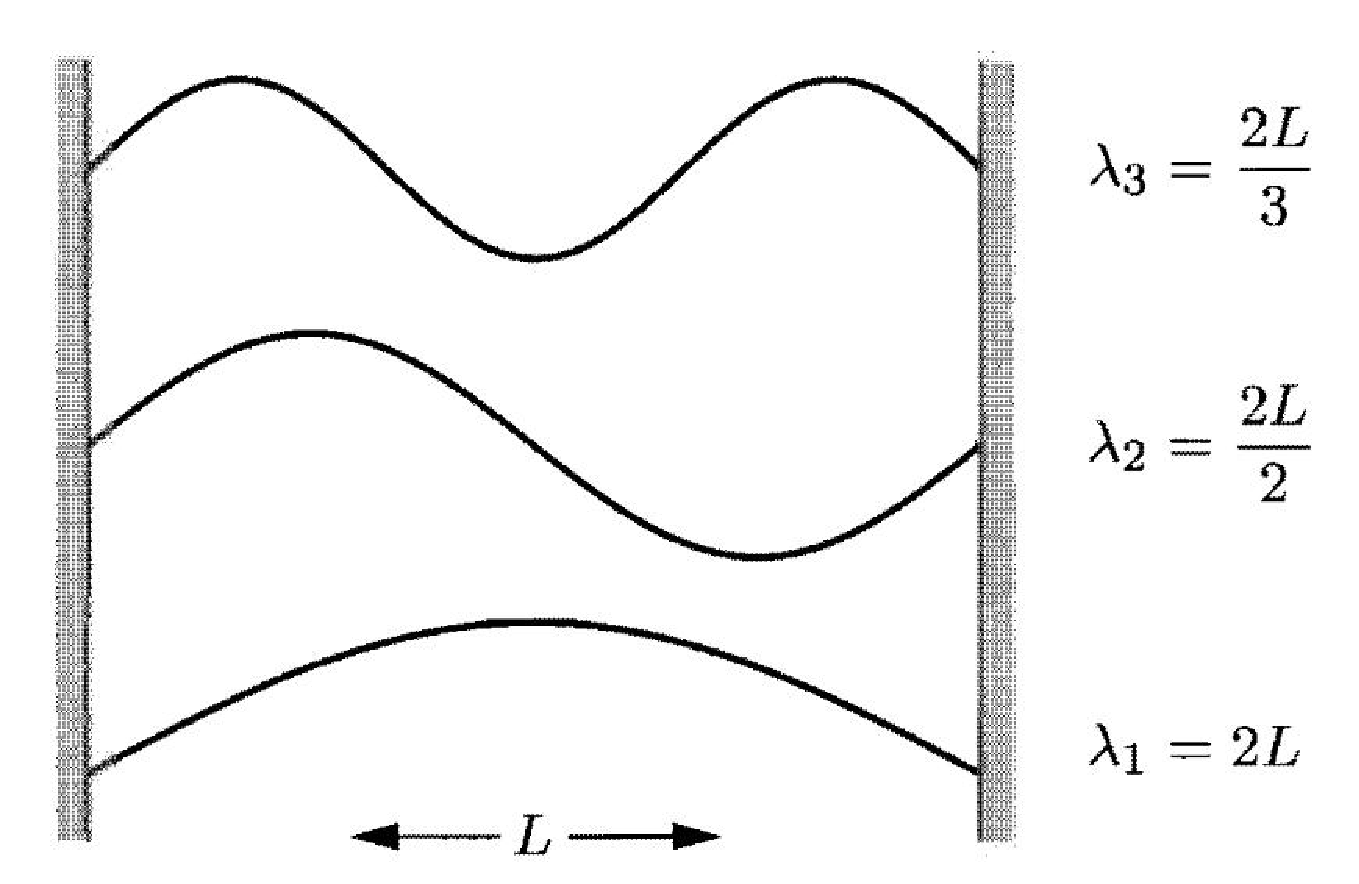
\includegraphics[width=0.65\textwidth]{figs/unit08_wavelengths.pdf}\end{center}

Specifically, the length $L$ must be an integer multiple of half a wavelength,
\begin{equation*}
  L = k \frac{\la}{2} \qquad \Lra \qquad c = \frac{L}{k} \frac{\om}{\pi} = \frac{\om}{\frac{\pi}{L} k},
\end{equation*}
and we can rewrite \eq{eq:photon_Ek} as
\begin{equation}
  \label{eq:photon_omega}
  \Eph(\om) = \hbar \om.
\end{equation}
Since $\la \propto c / \om$, we can observe the relation between length and energy scales mentioned above, in the discussion of Heisenberg's uncertainty principle.
Low (\textit{infrared}) frequencies correspond to small energies and long wavelengths, while high (\textit{ultraviolet}) frequencies correspond to large energies and short wavelengths.

We are now ready to write down the grand-canonical potential for a photon gas:
\begin{equation*}
  \Phi_{\text{ph}} = T \sum_{\ell = 0}^{\cL} \log\left[1 - e^{-\be (E_{\ell} - \mu)}\right] = 2T \sum_{\vec k} \log\left[1 - e^{-\be (\Eph(k) - \mu)}\right],
\end{equation*}
where the factor of $2$ in the final expression accounts for the doubly degenerate energy levels.
We can simplify this expression by appreciating that photons are easy to create and absorb. % TODO: Make sure it's clear that vanishing chemical potential enables large fluctuations in particle number...
For example, every time a light is turned on, it starts emitting a constant flood of photons (with wavelengths of several hundred nanometres).
Similarly, food in a microwave oven gets hot by absorbing many lower-energy photons (with longer wavelengths around $12$~centimetres).
In general an enormous number of photons is required to make even a small change in energy, so that \eq{eq:mu_E} implies the chemical potential of a photon gas is negligible,\footnote{If you are not convinced by the argument leading to this conclusion, you can find alternative analyses in Section~VI.C of ``\href{https://canvas.liverpool.ac.uk/courses/76365/files/12294000}{The elusive chemical potential}'' by Ralph Baierlein.}
\begin{equation*}
  \mu = \left.\pderiv{E}{N}\right|_S \approx 0 \qquad \Lra \qquad \Phi_{\text{ph}} \approx 2T \sum_{\vec k} \log\left[1 - e^{-\be \Eph(k)}\right].
\end{equation*}
Since we have $k_{x, y, z} \geq 1$, the strictly positive energies $\Eph(k) \propto k / L > 0$ ensure Bose--Einstein statistics is still convergent even with $\mu = 0$.

Another simplification comes from considering the photon gas in a volume that is large compared to the typical wavelengths of the photons. % Can expect to have some long-wavelength photons but not much effect from them due to their low energy...
Then the energies $\Eph(k) \propto k / L$ are very closely spaced, and we can approximate the sums over integer $k_{x, y, z}$ as integrals over continuous real $\khat_{x, y, z}$,\footnote{We mentioned this approximation in a footnote in \secref{sec:regulate}, and you can find further discussion in Section~6.7 of Dan Schroeder's \textit{Introduction to Thermal Physics}.} % TODO: Mention Poisson resummation?...
\begin{equation*}
  \Phi_{\text{ph}} \approx 2T \int \log\left[1 - e^{-\be \Eph(\khat)}\right] \d{\khat_x} \d{\khat_y} \d{\khat_z}.
\end{equation*}
Since the energy $\Eph(\khat)$ depends only on the magnitude $\khat$, we can profit from converting to spherical coordinates.
When we do so, we have to keep in mind that $k_{x, y, z} > 0$ corresponds to the positive octant of the sphere,
\begin{equation*}
  \int_0^{\infty} d\khat_x \int_0^{\infty} d\khat_y \int_0^{\infty} d\khat_z = \int_0^{\infty} \khat^2 \d{\khat} \int_0^{\pi / 2} \sin\theta \d{\theta} \int_0^{\pi / 2} d\phi = \frac{\pi}{2} \int_0^{\infty} \khat^2 \d{\khat},
\end{equation*}
so that
\begin{equation*}
  \Phi_{\text{ph}} \approx \pi T \int_0^{\infty} \khat^2 \log\left[1 - e^{-\be \Eph(\khat)}\right] \d{\khat}.
\end{equation*}
We can finally change variables to integrate over the angular frequency $\om = c \frac{\pi}{L} k$, with $\Eph = \hbar \om$, to find
\begin{equation}
  \label{eq:photon_grand}
  \Phi_{\text{ph}} \approx \pi T \left(\frac{L}{c \pi}\right)^3 \int_0^{\infty} \om^2 \log\left[1 - e^{-\be \hbar \om}\right] \d{\om} = \frac{VT}{\pi^2 c^3} \int_0^{\infty} \om^2 \log\left[1 - e^{-\be \hbar \om}\right] \d{\om},
\end{equation}
recognizing $L^3 = V$.
With this grand-canonical potential derived, we just need to take the appropriate derivatives to determine the thermodynamics and equation of state for the photon gas.
% ------------------------------------------------------------------



% ------------------------------------------------------------------
\newpage % TODO: Hack to push footnotes down to bottom of previous page...
\subsection{\label{sec:planck}The sun and the void}
It will be very interesting to use $\Phi_{\text{ph}}$ in \eq{eq:photon_grand} to analyse the average internal energy for a photon gas.
With $\mu = 0$, \eq{eq:E_grand} from \secref{sec:grand_pot} becomes
\begin{equation*}
  \vev{E}_{\text{ph}} = -T^2 \pderiv{}{T} \left[\frac{\Phi_{\text{ph}}}{T}\right] = \pderiv{}{\be} \left[\be \Phi_{\text{ph}}\right].
\end{equation*}
To begin, let's consider the energy density, as an integral over photon frequencies:
\begin{equation*}
  \frac{\vev{E}_{\text{ph}}}{V} = \int_0^{\infty} P(\om) \d{\om},
\end{equation*}
where the function $P(\om)$ is known as the \textit{spectral density}, or simply the \textit{spectrum}.
(It's not the pressure!)
What is the spectrum for a photon gas?
\begin{mdframed}
  \ \\[150 pt]
\end{mdframed}

You should find
\begin{equation}
  \label{eq:Planck_omega}
  P(\om) = \left(\frac{\hbar}{\pi^2 c^3}\right) \frac{\om^3}{e^{\be \hbar \om} - 1},
\end{equation}
which is known as the Planck spectrum, named after Max Planck.
We can equally well consider the Planck spectrum $P(\la)$ as a function of the wavelength $\la = 2\pi c / \om$, by changing variables in the expression above:
\begin{mdframed}
  \ \\[150 pt]
\end{mdframed}

You should find
\begin{equation}
  \label{eq:Planck_la}
  P(\la) = \left(\frac{16\pi^2 \hbar c}{\la^5}\right) \frac{1}{e^{2\pi\be \hbar c / \la} - 1},
\end{equation}
which is plotted for three temperatures $T = 1 / \be$ in the figure below, which comes from \href{https://commons.wikimedia.org/wiki/File:Black_body.svg}{Wikimedia Commons}.
(The plot divides our $P(\la)$ by $4\pi$~steradian and multiplies it by $c$ to convert from a spectral density to a spectral power per unit area per unit of solid angle.  For our purposes only the functional form is significant.) \\[-24 pt]
\begin{center}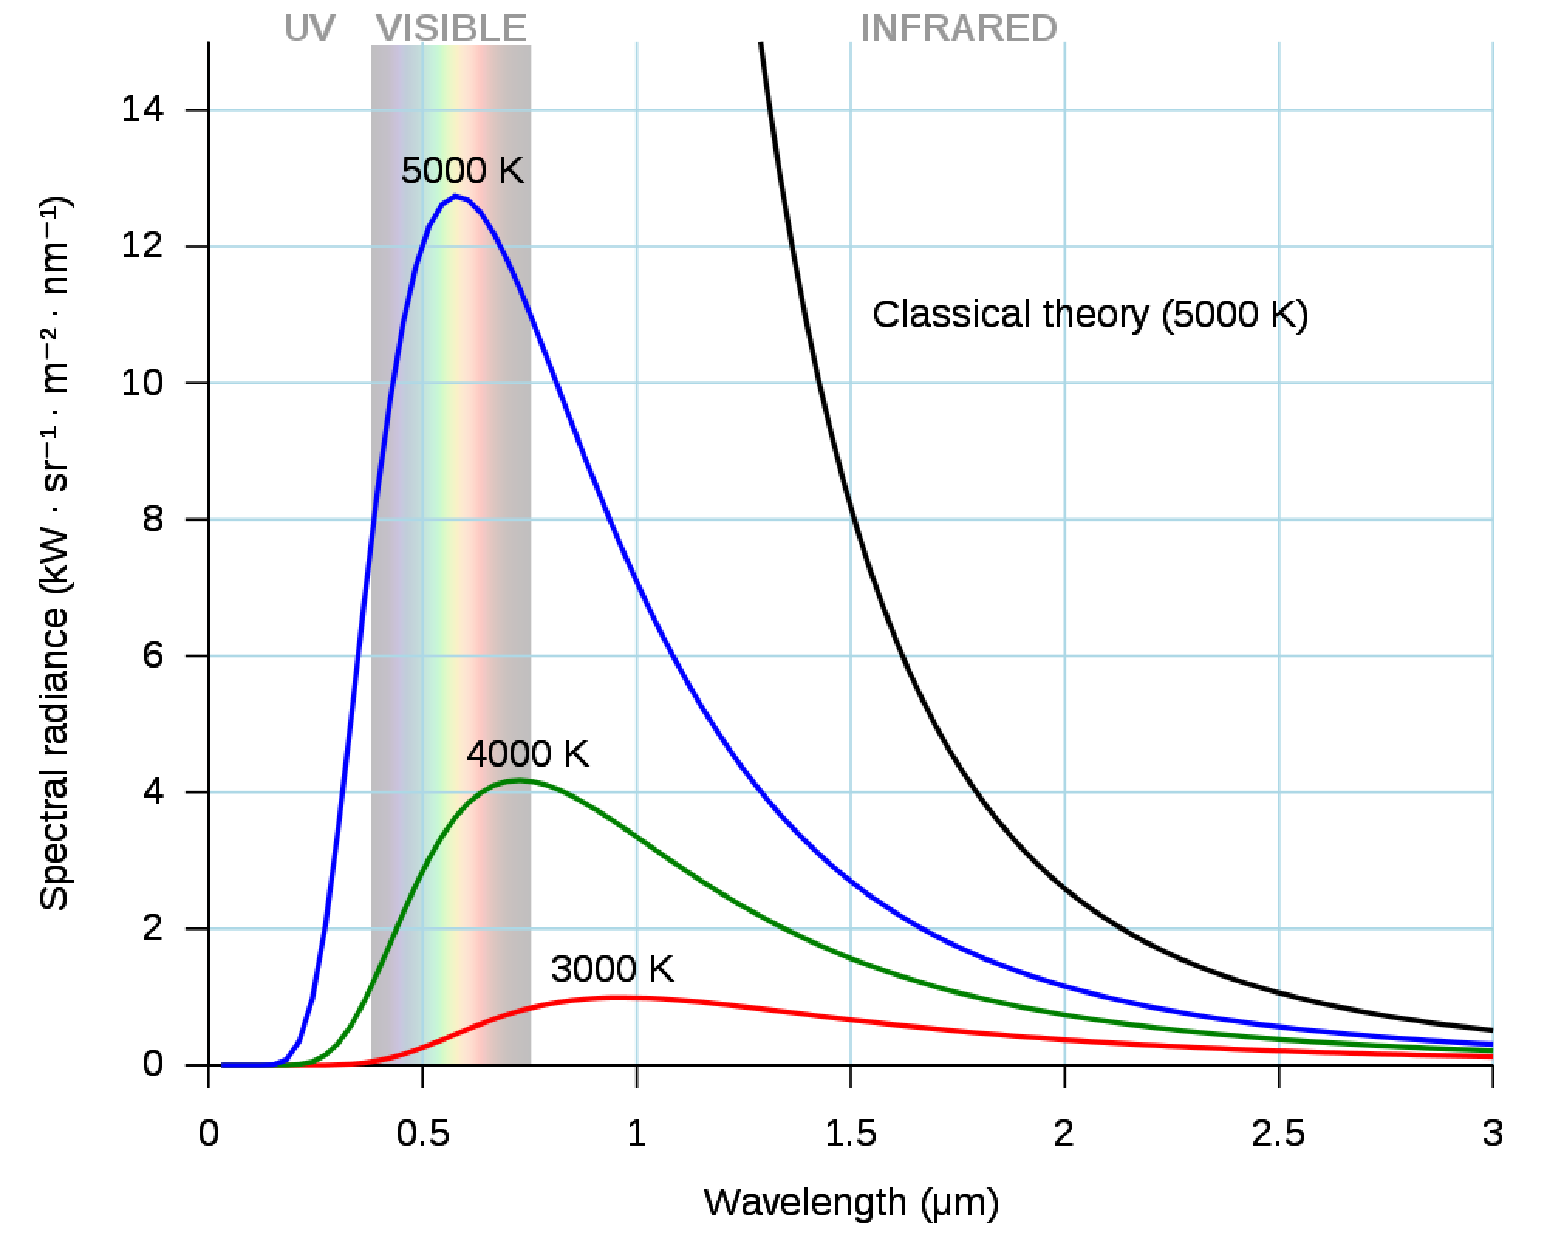
\includegraphics[width=0.8\textwidth]{figs/unit08_spectrum.pdf}\end{center}

Considering the high-energy ultraviolet (UV) limit of short wavelengths $\la$, we can see from \eq{eq:Planck_la} that $P(\la)$ is exponentially suppressed, which overwhelms the diverging factor $\propto 1 / \la^5$ in parentheses.
In the low-energy infrared (IR) limit, the large $\la$ has the same effect that a large temperature ($\be \ll 1$) would have: $e^{2\pi\be \hbar c / \la} - 1 \approx 2\pi\be \hbar c / \la$ and
\begin{equation*}
  P(\la) \approx \left(\frac{16\pi^2 \hbar c}{\la^5}\right) \frac{\la}{2\pi\be \hbar c} = \frac{8\pi T}{\la^4}.
\end{equation*}
The connection to large temperatures indicates that this is what classical statistical mechanics would predict for the spectrum of light.
It is known as the Rayleigh--Jeans spectrum, named after \href{https://en.wikipedia.org/wiki/John_William_Strutt,_3rd_Baron_Rayleigh}{the third Baron Rayleigh} and \href{https://en.wikipedia.org/wiki/James_Jeans}{James Jeans}.
Recall that the classical approach sums over all possible energies for each degree of freedom, corresponding to a light-emitting object (historically known as a \textit{black body}) emitting light of all wavelengths $\la$.
According to the classical Rayleigh--Jeans spectrum, in the limit $\la \to 0$ this light would carry an infinite amount of energy, a problem that became known as the \textit{ultraviolet catastrophe}.
Planck described his 1900 derivation of the UV-suppressed $P(\la)$ as ``an act of desperation'' to avoid this problem; it turned out to be one of the first steps towards quantum physics.

Another noteworthy feature of the Planck spectrum shown above is that as the temperature increases, the maximum of $P(\la)$ moves to shorter wavelengths and correspondingly larger energies.
It is not a coincidence that the peak of the spectrum for $T \approx 5000$~K falls within the wavelengths of visible light, roughly $400$--$700$~nm.
As shown in the figure below, also from \href{https://commons.wikimedia.org/wiki/File:Solar_spectrum_en.svg}{Wikimedia Commons}, the amount of sunlight that reaches the surface of the earth is also largest for visible wavelengths, which are visible to us because we have evolved to use this sunlight.

Taking into account the absorption of some sunlight by molecules in the atmosphere, we can see from the figure below that the energy spectrum of the sunlight reaching the top of the atmosphere is quite close to a Planck (or `blackbody') spectrum with temperature $T \approx 5778$~K.
The agreement isn't perfect, which is to be expected since the Planck spectrum relies on the non-trivial assumption of an ideal gas of non-interacting particles.
Despite that caveat, numerically fitting the measured sunlight to the Planck spectrum is how this `effective' surface temperature of the sun is determined.
This same fitting procedure can even be done for distant stars, with red stars corresponding to relatively low temperatures $T \lesssim 3500$~K and blue stars corresponding to relatively high temperatures $T \gtrsim 10\,000$~K. \\[-24 pt]
\begin{center}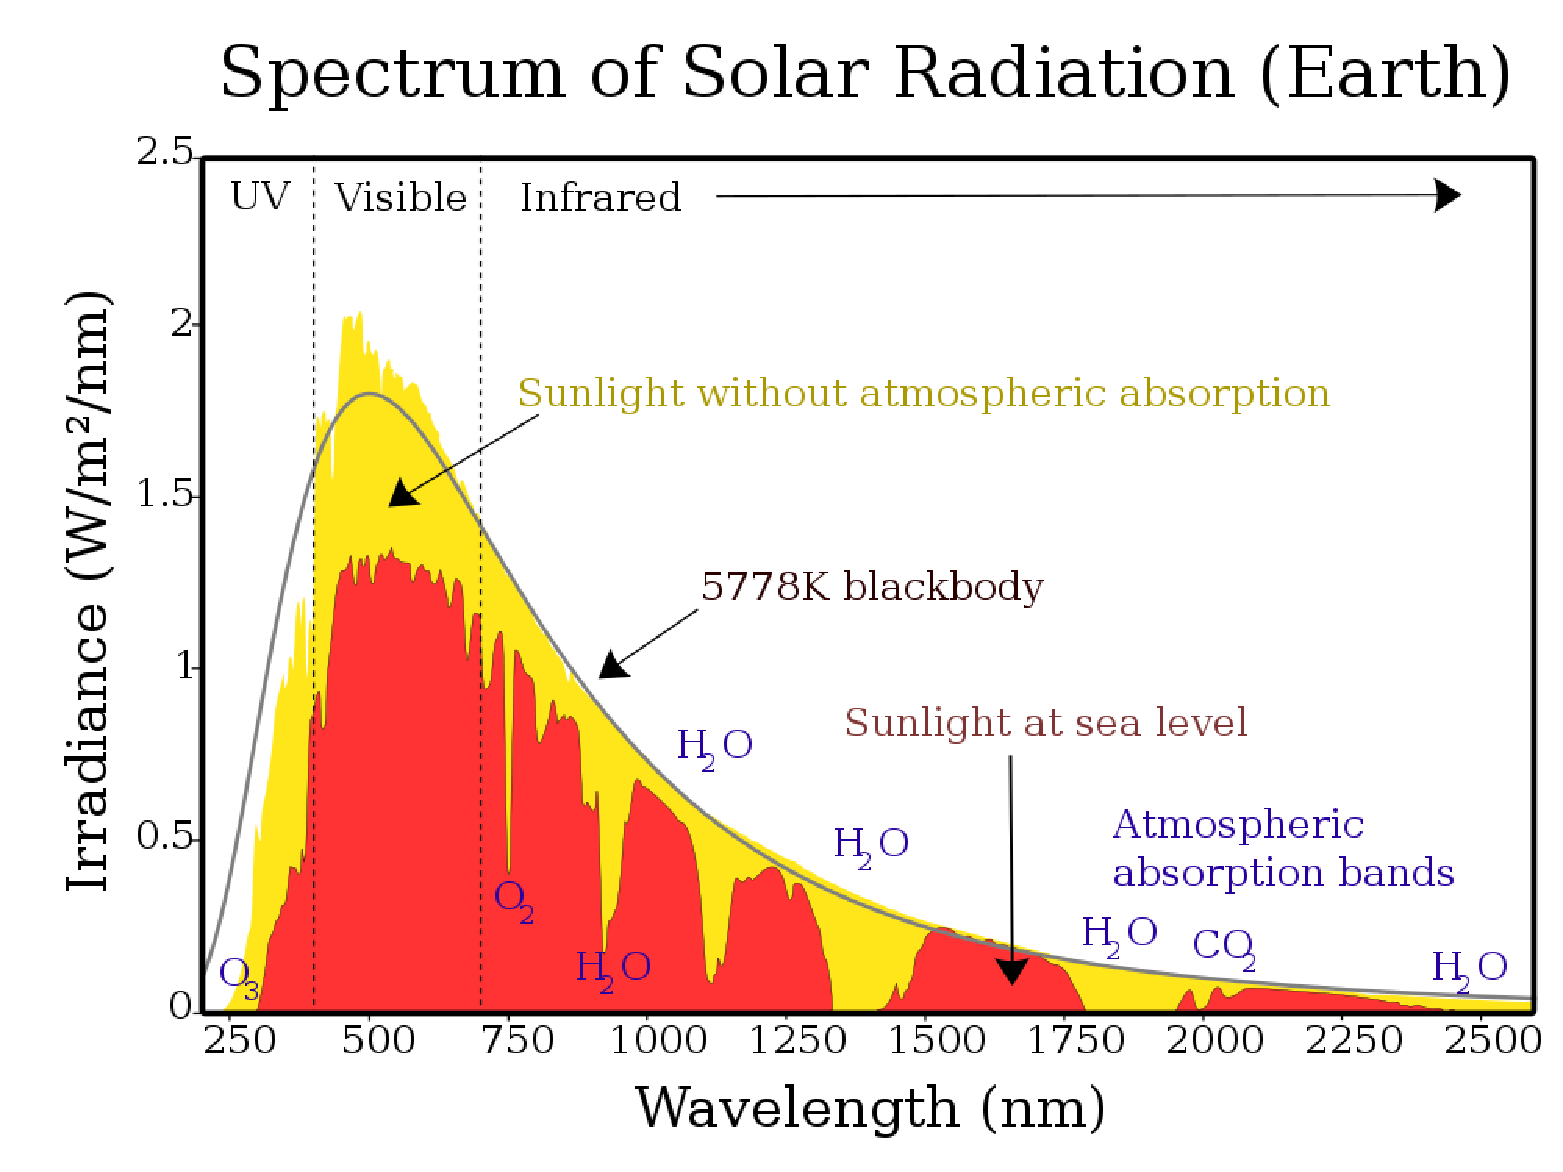
\includegraphics[width=0.8\textwidth]{figs/unit08_sun.pdf}\end{center}

Even more remarkably, we can use the Planck spectrum to determine the temperature of intergalactic space.
Rather than being empty, these voids are actually permeated by a very low-temperature photon gas left over from the Big Bang roughly $14$~billion years ago.
This photon gas is known as the \href{https://en.wikipedia.org/wiki/Cosmic_microwave_background}{cosmic microwave background} (CMB), and carries information about the early evolution of the universe, including some of the strongest evidence for the existence of dark matter.

The picture below is a famous visualization of the CMB, provided by the \href{http://www.esa.int/ESA_Multimedia/Images/2013/03/Planck_CMB}{European Space Agency} and produced from measurements taken by their `Planck' satellite. % Can compare with WMAP from wmap.gsfc.nasa.gov/media/101080/
For each point in the sky the satellite measures the photon spectrum reaching it from that direction.
The contributions from stars and galaxies are subtracted, and the remaining data are fit to the Planck spectrum to find the temperature of the intergalactic CMB photon gas at that point.
From point to point, there are only small temperature fluctuations around the average $T_{\text{CMB}} \approx 2.725$~K.
That average temperature is subtracted and the fluctuations themselves are shown below, with warmer red-coloured regions only $\De T \approx 0.0002$~K hotter than the cooler blue-coloured regions. \\[-24 pt]
\begin{center}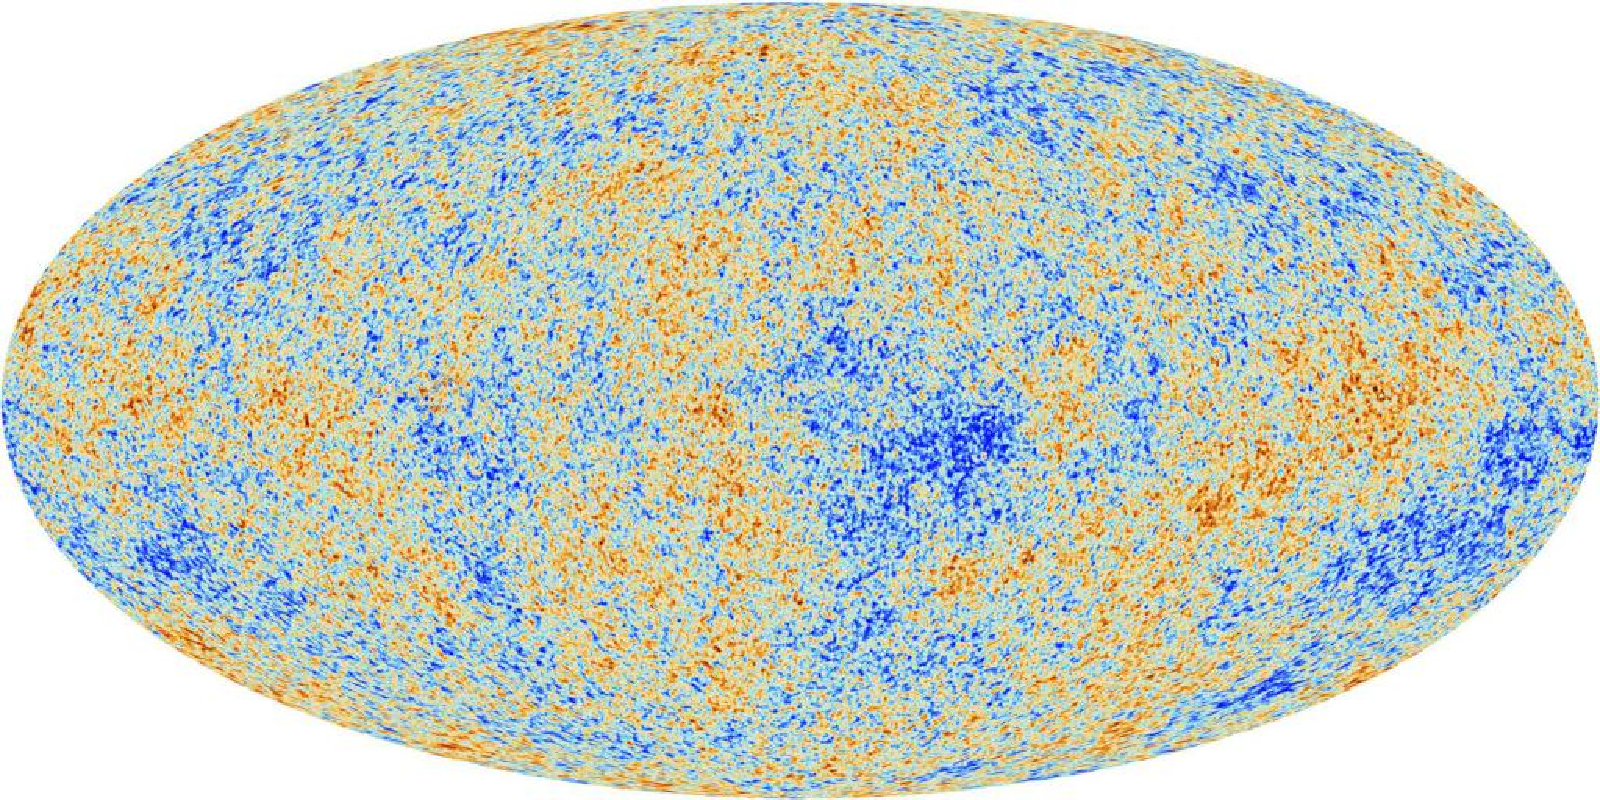
\includegraphics[width=0.8\textwidth]{figs/unit08_CMB.pdf}\end{center}

The final figure below illustrates such a fit of CMB data to the Planck spectrum, using measurements taken by the Cosmic Background Explorer (COBE) satellite and \href{https://doi.org/10.1086/185717}{published in 1990}.
(This version of the figure is adapted from that publication, and copied from Schroeder's \textit{Introduction to Thermal Physics}.)
The squares are the measured data, and their size represents a cautious estimate of uncertainties.
They are plotted with the frequency $f = \om / (2\pi)$ on the horizontal axis, where $f \approx 3\times 10^{11}~\text{s}^{-1}$ corresponds to a low-energy wavelength $\la = c / f \approx 1$~mm, roughly $1000$ times longer than the wavelengths of visible light.
The solid line is a fit to the data, which produces $T_{\text{CMB}} = 2.735 \pm 0.060$~K.
While more recent satellites have increased the precision with which we know $T_{\text{CMB}}$, this first result was awarded the 2006 Nobel Prize in Physics. \\[-24 pt]
\begin{center}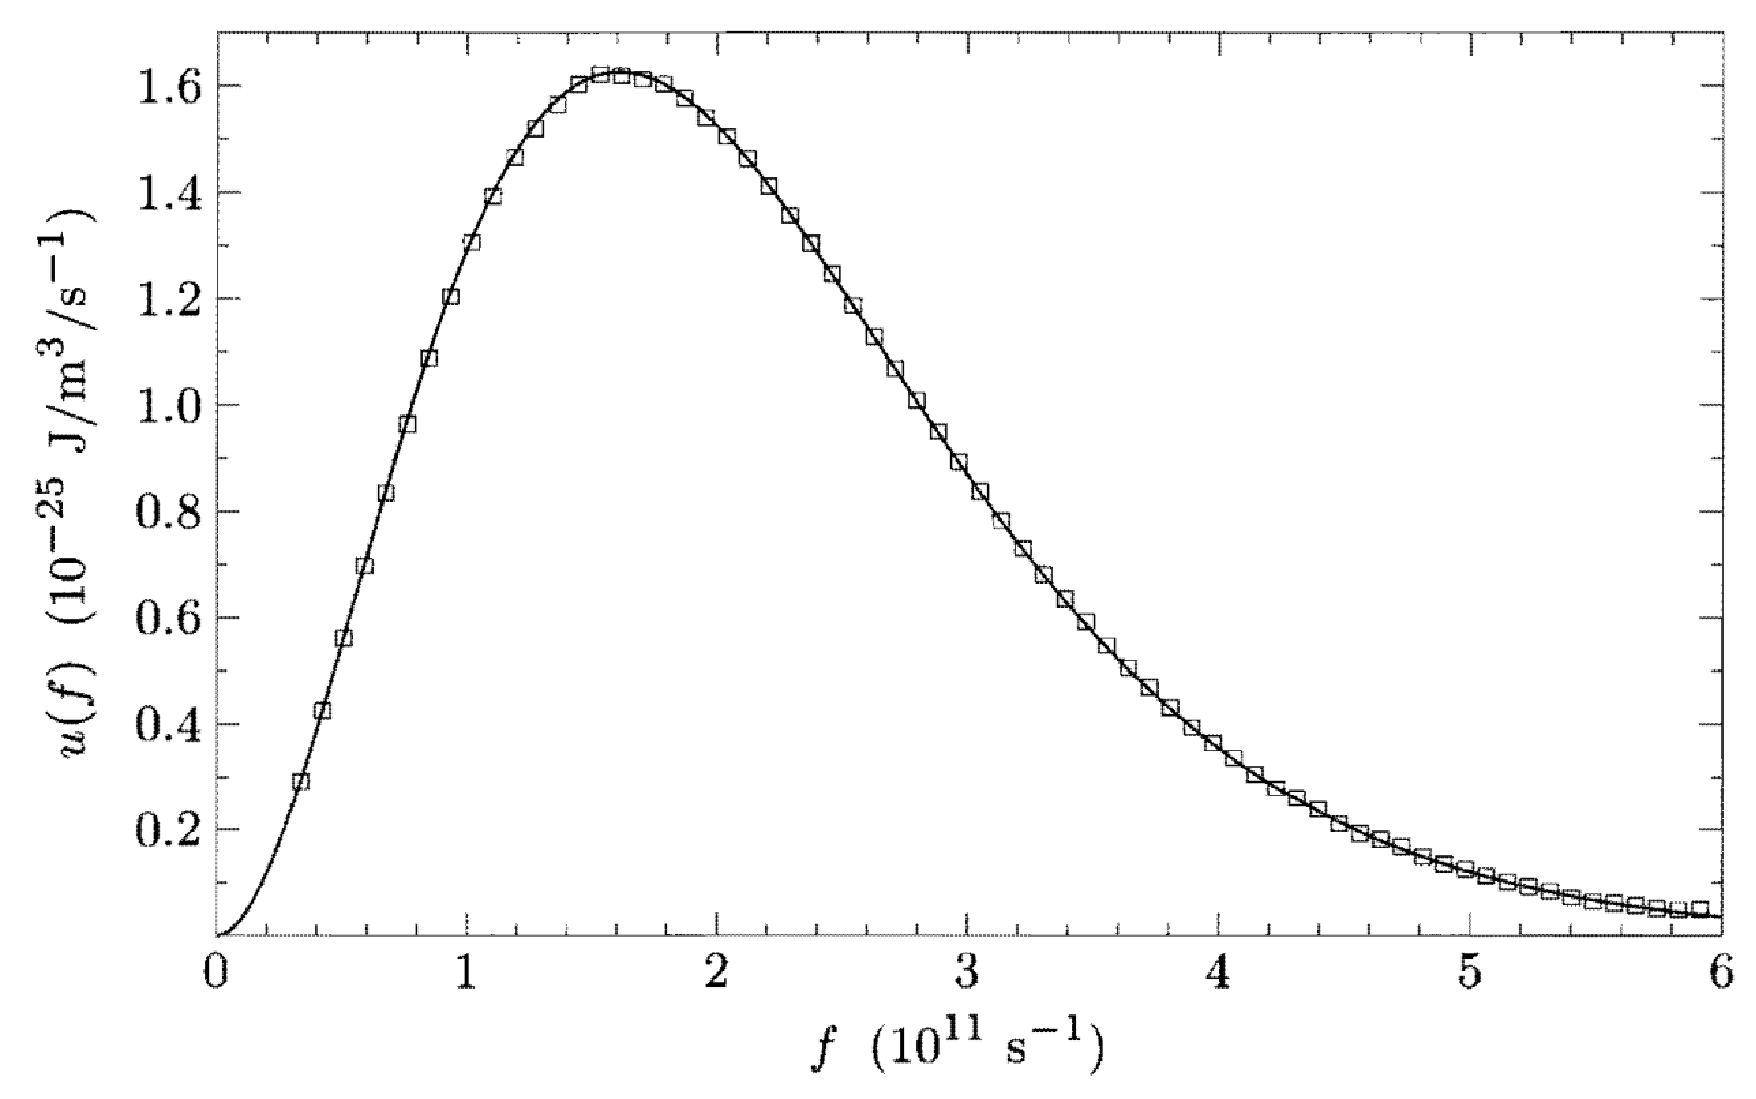
\includegraphics[width=0.8\textwidth]{figs/unit08_COBE.pdf}\end{center}

\begin{shaded}
  Even though we derived the Planck spectrum by assuming an ideal gas of non-interacting photons, we see that it provides an excellent mathematical model for real physical systems, stretching from the hottest to the coldest places in the universe.
\end{shaded}
% ------------------------------------------------------------------



% ------------------------------------------------------------------
\subsection{\label{sec:photon_eos}Equation of state for the photon gas}
Having looked in some detail at the integrand for the photon gas energy density, \eq{eq:Planck_omega}, let's complete the integration, which is related to the Riemann zeta function:
\begin{equation*}
  \int_0^{\infty} \frac{x^3}{e^x - 1} \d{x} = \Gamma(4) \zeta(4) = \frac{\pi^4}{15}.
\end{equation*}
Using this result, what is the average energy density for an ideal photon gas?
\begin{mdframed}
  \ \\[85 pt]
\end{mdframed}

You should find a result proportional to $T^4$, which appears significantly more complicated than \eq{eq:ideal_energy} for the energy of an $N$-particle non-relativistic ideal gas in the canonical ensemble.
This is related to the fluctuating particle number now that we are working in the grand-canonical ensemble.
It's possible to simplify the current situation by computing the average photon number from \eq{eq:N_grand},
\begin{equation*}
  \vev{N}_{\text{ph}} = -\left. \pderiv{}{\mu} \Phi_{\text{ph}}\right|_{\mu = 0} = -\left. \frac{VT}{\pi^2 c^3} \int_0^{\infty} \om^2 \pderiv{}{\mu} \log\left[1 - e^{-\be \hbar \om} e^{\be \mu}\right] \d{\om} \right|_{\mu = 0},
\end{equation*}
recalling $\mu = 0$ for photon gases.
The calculation is quite similar to that for the average internal energy density, now involving the integral
\begin{equation*}
  \int_0^{\infty} \frac{x^2}{e^x - 1} \d{x} = \Gamma(3) \zeta(3) = 2\zeta(3).
\end{equation*}
Using this result, what is the average particle number density for an ideal photon gas?
\begin{mdframed}
  \ \\[80 pt]
\end{mdframed}

You should find a result proportional to $VT^3 \propto \vev{E}_{\text{ph}} / T$, so that
\begin{equation}
  \label{eq:photon_gas_energy}
  \vev{E}_{\text{ph}} = \frac{\pi^2}{15 \hbar^3 c^3} VT^4 = \frac{\pi^4}{30\zeta(3)} \vev{N}_{\text{ph}} T.
\end{equation}
The functional form is the same as \eq{eq:ideal_energy}, with a larger numerical factor
\begin{equation*}
  \frac{\pi^4}{30\zeta(3)} = \frac{\Gamma(4) \zeta(4)}{\Gamma(3) \zeta(3)} \approx 2.7
\end{equation*}
compared to $\frac{3}{2}$ for the classical non-relativistic case.

To get the rest of the way to the equation of state for the photon gas, we need to compute the \textit{radiation pressure}
\begin{equation*}
  P_{\text{ph}} = -\left. \pderiv{}{V} \vev{E}_{\text{ph}} \right|_{S_{\text{ph}}},
\end{equation*}
which requires first figuring out the condition of constant entropy $S_{\text{ph}}$ for a photon gas.
From \eq{eq:grand_relation} with $\mu = 0$, we have
\begin{equation*}
  S_{\text{ph}} = \frac{\vev{E}_{\text{ph}} - \Phi_{\text{ph}}}{T}.
\end{equation*}
Looking back to \eq{eq:photon_grand} for the grand-canonical potential, we see
\begin{equation*}
  \frac{\Phi_{\text{ph}}}{T} = \frac{V}{\pi^2 c^3} \int_0^{\infty} \om^2 \log\left[1 - e^{-\be \hbar \om}\right] \d{\om} = \frac{VT^3}{\pi^2 \hbar^3 c^3} \int_0^{\infty} x^2 \log\left[1 - e^{-x}\right] \d{x},
\end{equation*}
changing variables to $x = \be \hbar \om = \hbar \om / T$.
The final factor in this expression is yet another delightful integral,
\begin{equation*}
  \int_0^{\infty} x^2 \log\left[1 - e^{-x}\right] \d{x} = -2\zeta(4) = -\frac{\pi^4}{45}.
\end{equation*}
Since this gives us $S \propto VT^3$, we can conclude that the condition of constant entropy for a photon gas is $V T^3 = \mbox{constant}$, in contrast to the $V T^{3/2}$ dependence of \eq{eq:ideal_entropy} for classical non-relativistic particles.

At this point it is straightforward to take the derivative of the average internal energy if we express the constant-entropy condition as $T = b V^{-1 / 3}$, with $b$ a constant:
\begin{mdframed}
  \ \\[120 pt]
\end{mdframed}
For the resulting equation of state for the photon gas, you should find
\begin{equation}
  \label{eq:photon_eos}
  P_{\text{ph}} V = \frac{1}{3} \vev{E}_{\text{ph}} = \frac{\pi^4}{90\zeta(3)} \vev{N}_{\text{ph}} T.
\end{equation}
The functional form is the same as the (classical, non-relativistic) ideal gas law, with just an additional numerical factor of
\begin{equation*}
  \frac{\pi^4}{90\zeta(3)} = \frac{\zeta(4)}{\zeta(3)} \approx 0.9004.
\end{equation*}
% ------------------------------------------------------------------



% ------------------------------------------------------------------
\subsection{\label{sec:fermi_nonrel}Non-relativistic ideal fermion gas}
For the remainder of this unit we will apply the grand-canonical ensemble to investigate ideal gases of non-interacting fermions.
We again take the approach of quantum statistics, defining micro-states by summing over the possible occupation numbers $n_{\ell}$ for each energy level $\cE_{\ell}$ with (possibly not unique) energy $E_{\ell}$.
In contrast to the bosonic case considered above, the only possible occupation numbers are now $n_{\ell} = 0$ and $1$, since the Pauli exclusion principle prevents multiple identical fermions from occupying the same energy level.

In \secref{sec:fermi} we derived the grand-canonical partition function (\eq{eq:partfunc_FD}) that defines quantum Fermi--Dirac statistics for systems of non-interacting fermions,
\begin{equation*}
  \ZFD(\be, \mu) = \prod_{\ell = 0}^{\cL} \left[1 + e^{-\be (E_{\ell} - \mu)}\right],
\end{equation*}
in terms of the inverse temperature $\be = 1 / T$ and chemical potential $\mu$.
Recall that it is possible for systems of fermions to have any value for the chemical potential, either positive or negative, in contrast to the systems of bosons we considered above.
From the corresponding grand-canonical potential,
\begin{equation*}
  \Phi_{\text{FD}} = -T\log \ZFD = -T \sum_{\ell = 0}^{\cL} \log\left[1 + e^{-\be (E_{\ell} - \mu)}\right]
\end{equation*}
we can determine the large-scale properties of the system, including its average internal energy $\vev{E}$, average particle number $\vev{N}$, entropy $S$, and pressure $P$, along with the equation of state relating these quantities.

Concrete calculations require specifying the energy levels of the system, including the degeneracies of any distinct energy levels $\left\{\cE_m, \cE_n\right\}$, $m \neq n$, with the same energy $E_m = E_n$.
In this section we'll consider non-relativistic particles, expanding on our review of such systems in \secref{sec:photon}.
In a volume $V = L^3$, the energy levels are defined by the non-zero quantized energies
\begin{align*}
  E(k) & = \eps \left(k_x^2 + k_y^2 + k_z^2\right) \qquad &
  \eps & \equiv \frac{\hbar^2 \pi^2}{2mL^2} \qquad &
  k_{x, y, z} & = 1, 2, \cdots.
\end{align*}
In addition to the usual degeneracies coming from permutations of $(k_x, k_y, k_z)$ that we have already analysed, for each distinct $\vec k$ typical fermions such as electrons have two degenerate energy levels with the same energy $E(k)$.
This arises from a quantum property called \textit{spin}, rather than the two polarizations for photons discussed in \secref{sec:photon}: `spin-up' and `spin-down' electrons with everything else the same (including their energies) occupy distinct, degenerate energy levels.
This property of spin is related to the spin--statistics theorem mentioned in \secref{sec:spin}, and is another topic we can discuss further in a tutorial if there is interest.
For our statistical mechanics purposes it will suffice simply to incorporate this information into our ansatz as input.

Thus the grand-canonical potential for an ideal gas of non-relativistic fermions is
\begin{equation*}
  \Phi_{\text{f}} = -T \sum_{\ell = 0}^{\cL} \log\left[1 + e^{-\be (E_{\ell} - \mu)}\right] = -2T \sum_{\vec k} \log\left[1 + \exp\left(-\frac{\hbar^2 \pi^2 k^2}{2mL^2 T} + \frac{\mu}{T}\right)\right].
\end{equation*}
We can again proceed by considering the gas in a large volume and approximating the sum over discrete integer $k_{x, y, z}$ by integrals over continuous real $\khat_{x, y, z}$:
\begin{equation*}
  \Phi_{\text{f}} \approx -2T \int \log\left[1 + \exp\left(-\frac{\hbar^2 \pi^2 \khat^2}{2mL^2 T} + \frac{\mu}{T}\right)\right] \d{\khat_x} \d{\khat_y} \d{\khat_z}.
\end{equation*}
Converting to spherical coordinates and carrying out the angular integrations over the $\frac{\pi}{2}$ solid angle of the octant of the sphere with $k_{x, y, z} > 0$, we have
\begin{equation*}
  \Phi_{\text{f}} \approx -\pi T \int_0^{\infty} \khat^2 \log\left[1 + \exp\left(-\frac{\hbar^2 \pi^2 \khat^2}{2mL^2 T} + \frac{\mu}{T}\right)\right] \d{\khat}.
\end{equation*}
In the same spirit as the change of variables we carried out to integrate over photon frequencies $\om$, let's now work in terms of the fermion energy $E = \displaystyle \frac{\hbar^2 \pi^2}{2mL^2}\khat^2$:
\begin{mdframed}
  \ \\[100 pt]
\end{mdframed}

As for the case of a photon gas, \eq{eq:photon_grand}, you should find $\Phi_{\text{f}} \propto VT$.
It will be convenient to keep this grand-canonical potential in the form of an integral over the energy $E$, which we will evaluate after taking appropriate derivatives to determine the thermodynamics and equation of state for non-relativistic fermions.
% ------------------------------------------------------------------



% ------------------------------------------------------------------
\subsection{\label{sec:fermi_lowT}Low-temperature equation of state}
In contrast to the photon gas, we need to retain the chemical potential in our analyses of non-relativistic fermions, which makes these calculations more complicated.
To achieve a different simplification, we can focus on the low-temperature regime where we expect quantum Fermi--Dirac statistics to differ significantly from the classical case we considered back in \secref{sec:regulate}.
As we saw in \secref{sec:quantum_classical}, it is only at high temperatures, with large negative chemical potential, that the classical approach provides a good approximation to the true quantum physics.

To see how low temperatures simplify the analysis of the non-relativistic fermion gas, it will prove profitable to first consider the average particle number
\begin{equation*}
  \vev{N}_{\text{f}} = -\pderiv{}{\mu} \Phi_{\text{f}},
\end{equation*}
using the grand-canonical potential we computed above.
In analogy to the Planck spectrum we derived for the photon gas in \secref{sec:planck}, we first express the average particle number density as an integral over energies,
\begin{equation}
  \label{eq:N_fermi}
  \frac{\vev{N}_{\text{f}}}{V} = \frac{\sqrt{2m^3}}{\pi^2 \hbar^3} \int_0^{\infty} F(E) \sqrt{E} \d{E},
\end{equation}
where the function $F(E)$ is known as the Fermi function.
In contrast to the Planck spectrum, some constant factors are kept separate from $F(E)$, so that it more closely resembles the average occupation numbers $\vev{n_{\ell}}$ we computed in \secref{sec:quantum_classical}:
\begin{mdframed}
  \ \\[100 pt]
\end{mdframed}

As usual in the grand-canonical approach, the average particle number density and Fermi function depend on the inverse temperature \be and the chemical potential $\mu$.
Expressing $F(E)$ in terms of the dimensionless ratios $E / \mu$ and $T / \mu$,
\begin{equation*}
  F(E) = \frac{1}{\exp\left[\frac{E - \mu}{T}\right] + 1} = \frac{1}{\exp\left[\frac{\mu}{T}\left(\frac{E}{\mu} - 1\right)\right] + 1} = \frac{1}{\left(\exp\left[\frac{E}{\mu} - 1\right]\right)^{\mu / T} + 1},
\end{equation*}
we can highlight the two main features of the figure on the next page, which plots the Fermi function against $E / \mu$ for various temperatures $T / \mu$.
Here we assume a positive chemical potential, $\mu > 0$, which we will soon show is required for low-temperature non-relativistic fermion gases.

First, we can see that the point $E = \mu$, where $F(E) = 1 / 2$ for any temperature, is a threshold at which the behaviour of the Fermi function changes.
For larger energies $E > \mu$, the factor $\exp\left[\frac{E}{\mu} - 1\right] > 1$ and drives $F(E) \to 0$ as the energy increases.
For smaller energies $E < \mu$, the factor $\exp\left[\frac{E}{\mu} - 1\right] < 1$ and becomes negligible if raised to a sufficiently large power $\frac{\mu}{T}$, leaving $F(E) \to 1$.
These two asymptotic limits reflect the possible energy level occupation numbers for fermions, $n_{\ell} = 0$ and $1$.
Second, smaller temperatures cause much more rapid approach to these two limits, with the exponential factor either enhanced (if $E > \mu$) or suppressed (if $E < \mu$) by a power $\mu / T \gg 1$. \\[-24 pt]
\begin{center}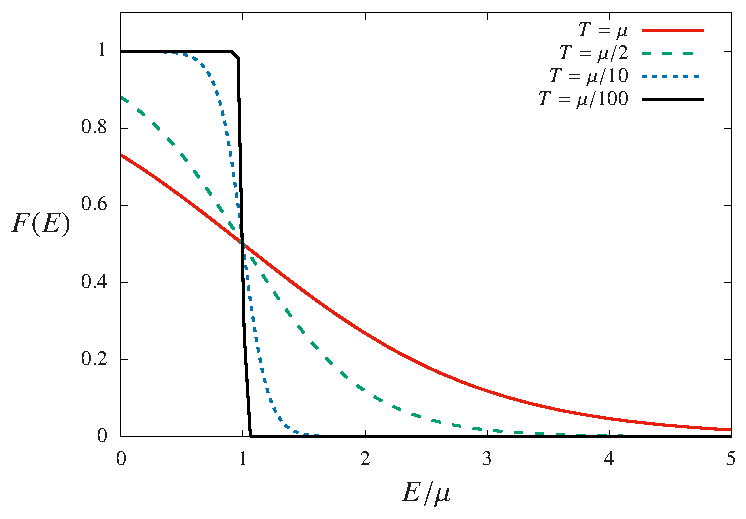
\includegraphics[width=0.8\textwidth]{figs/unit08_dist.pdf}\end{center}

Therefore, for small temperatures $T \ll \mu$, we can simplify our calculations by approximating the Fermi function as a step function,
\begin{equation}
  \label{eq:Fermi_step}
  F(E) \approx \left\{\begin{array}{l}1 \qquad \mbox{for } \ 0 \leq E < \mu \\
                                      0 \qquad \mbox{otherwise}\end{array}\right. .
\end{equation}
Using this approximation, what is the resulting average particle number density?
\begin{mdframed}
  \ \\[100 pt]
\end{mdframed}

You should find a result proportional to $\mu^{3 / 2}$ but independent of $T$.
The temperature independence turns out to be the leading-order behaviour of a more general result that can be organized in powers of $T / \mu \ll 1$, through a method known as the \textit{Sommerfeld expansion} (named after \href{https://en.wikipedia.org/wiki/Arnold_Sommerfeld}{Arnold Sommerfeld}).
The $\mu^{3 / 2}$ dependence on the chemical potential is something we could have predicted before doing the explicit calculation.
This is because the step function in \eq{eq:Fermi_step} corresponds to a single fermion occupying each and every energy level with $E_{\ell} < \mu$, while all energy levels with $E_{\ell} > \mu$ are unoccupied.
Since $E(k) \propto k^2$, summing over all $k_{x, y, z}$ for which $E(k) < \mu$ corresponds to computing (a portion of) the volume of a sphere of radius $r_k = \sqrt{\mu}$.
This volume is proportional to $r_k^3 = \mu^{3 / 2}$, in agreement with our result above.
Inverting that result defines the \textbf{Fermi energy}, the maximum fermion energy at zero temperature:
\begin{equation}
  \label{eq:Fermi_energy}
  E_F = \mu = \frac{\hbar^2}{2m}\left(\frac{3\pi^2 \vev{N}_{\text{f}}}{V}\right)^{2 / 3}.
\end{equation}
Like the step-function approximation to the Fermi function, this equality between the Fermi energy and the chemical potential is only exact at zero temperature, with $0 < T \ll E_F$ introducing small corrections discussed in \secref{sec:Sommerfeld}. % TODO: Could elaborate on Fermi energy as radius of energy sphere into which all N particles could be packed...

Let's compute the average energy density of the non-relativistic fermion gas at low temperatures.
Rather than taking another derivative of the grand-canonical potential, we can note from \eq{eq:total_energy_levels} and from our work on the photon gas in \secref{sec:photon_eos} that
\begin{equation}
  \frac{\vev{E}_{\text{f}}}{V} = \frac{\sqrt{2m^3}}{\pi^2 \hbar^3} \int_0^{\infty} E \; F(E) \sqrt{E} \d{E}.
\end{equation}
That is, instead of simply counting the number of fermions in the system, we need to add up their energies, introducing an extra factor of $E$ compared to \eq{eq:N_fermi}.
Still using the low-temperature step-function approximation for the Fermi function in \eq{eq:Fermi_step}, what is the average energy density?
\begin{mdframed}
  \ \\[100 pt]
\end{mdframed}
You should find
\begin{equation}
  \label{eq:fermi_E_N}
  \vev{E}_{\text{f}} = \frac{3}{5} \mu \vev{N}_{\text{f}},
\end{equation}
which means that the average energy of each fermion in the low-temperature ideal gas, $\vev{E}_{\text{f}} / \vev{N}_{\text{f}}$, is three-fifths of the Fermi energy $E_F = \mu$.

\begin{shaded}
  In particular, we find that ideal gases of non-relativistic fermions have positive internal energy even as the temperature approaches absolute zero, $T \to 0$.
\end{shaded}

This can be understood by recalling that the lowest-energy pair of degenerate energy levels can each hold only a single fermion, forcing any additional fermions to `fill' energy levels with larger energies $E_{\ell} > 0$, up to the Fermi energy.
It is a stark contrast to the $\vev{E} = \frac{3}{2} N T$ we found for classical ideal gases in the canonical ensemble in \eq{eq:ideal_energy}, as well as the $\vev{E}_{\text{ph}} \approx 2.7 \vev{N}_{\text{ph}} T \propto T^4$ we more recently computed in \eq{eq:photon_gas_energy} for a grand-canonical quantum gas of photons.
In both of those cases the average energy vanishes in the zero-temperature limit.
This is because all the particles in those classical and bosonic systems are able to occupy the lowest energy level at low temperatures, with exponentially small probabilities $\propto e^{-E_{\ell}/ T}$ for particles to occupy any energy levels with $E_{\ell} > E_0$.

This picture of fermions filling energy levels up to the Fermi energy also clarifies why the chemical potential for a fermion gas must be positive at low temperatures.
Recall \eq{eq:mu_E} for the chemical potential,
\begin{equation*}
  \mu = \left.\pderiv{E}{N}\right|_{S, V},
\end{equation*}
which we derived from the generalized thermodynamic identity in \secref{sec:grand_pot}.
Let's use this to consider what happens when we increase the number of particles in a zero-temperature fermion gas.
In this limit $T \to 0$, there is only the single quantum micro-state described above, with all energy levels filled below the Fermi energy $E_F$ and empty above $E_F$. % Ignore irrelevant complication from possibility that only a portion of the degenerate energy levels at $E_F$ are filled
Adding particles, $\De N > 0$, doesn't increase the number of accessible micro-states, and therefore doesn't increase the entropy $S_{\text{f}} = -\sum_{i = 1}^M p_i \log p_i = 0$, satisfying the constant-entropy condition required by this equation.
However, it does increase the energy, because the added particles must fill the first available energy levels, just above the Fermi energy.
That is, $\De E = E_F \De N > 0$, and we find $\mu = E_F > E_0 \geq 0$ as claimed earlier in this section.
It is an interesting but lengthy exercise (discussed in \secref{sec:Sommerfeld}) to show that the chemical potential becomes negative as the temperature increases and we approach the classical limit.

To get the rest of the way to the low-temperature equation of state for ideal gases of non-relativistic fermions, we need to compute the pressure
\begin{equation*}
  P_{\text{f}} = -\left. \pderiv{}{V} \vev{E}_{\text{f}} \right|_{N, S_{\text{f}}}.
\end{equation*}
As we just discussed, the single accessible micro-state for $T \to 0$ automatically satisfies the condition of constant entropy, $S_{\text{f}} = 0$.
Applying \eq{eq:Fermi_energy} that relates the chemical potential to the average particle number density, we have
\begin{equation*}
  \vev{E}_{\text{f}} = \frac{3}{5} \mu \vev{N}_{\text{f}} = \frac{3}{5} \left(\frac{\hbar^2}{2m}\right) \left(\frac{3\pi^2}{V}\right)^{2 / 3} \vev{N}_{\text{f}}^{5 / 3}.
\end{equation*}
This is all we need to determine the pressure, which we can relate to the energy density, the Fermi energy $E_F = \mu$ and the particle number density:
\begin{mdframed}
  \ \\[85 pt]
\end{mdframed}
In particular, we can see that the pressure (like the energy) remains positive even as the temperature approaches absolute zero, with
\begin{equation}
  \label{eq:degen_pressure}
  P_{\text{f}} = \left(3\pi^2\right)^{2 / 3} \frac{\hbar^2}{5m} \rho_{\text{f}}^{5 / 3},
\end{equation}
where we define the density $\rho_{\text{f}} = \vev{N}_{\text{f}} / V$.
This positive pressure in the $T \to 0$ limit is not due to any direct force between the fermions, which remain non-interacting in this ideal gas.
It is a purely quantum effect resulting from the Pauli exclusion principle.

As we saw earlier in this section, the temperature independence of the pressure $P_{\text{f}}$ is due to approximating the low-temperature Fermi function as a step function in \eq{eq:Fermi_step}, and systematic corrections to this approximation can be computed through a Sommerfeld expansion.
Even without getting into such detailed calculations, we know that in the high-temperature classical regime the quantum ideal gas of massive fermions will be well approximated by the classical ideal gas we considered in \secref{sec:ideal_gas}, with equation of state
\begin{equation}
  PV = NT \qquad \Lra \qquad P = \frac{N}{V} T = \rho T.
\end{equation}
In words, at high temperatures the pressure depends linearly on the temperature, with the slope corresponding to the density $\rho$.
The plot below (produced by \href{https://github.com/daschaich/MATH327_2025/blob/main/lecture_notes/unit08_pressure.py}{this Python code}) shows how the pressure changes from a positive constant as $T \to 0$ to this linear behaviour at higher temperatures. \\[-24 pt]
\begin{center}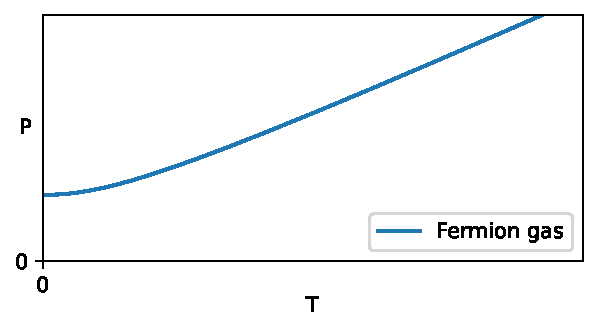
\includegraphics[width=0.8\textwidth]{figs/unit08_pressure.pdf}\end{center}
% ------------------------------------------------------------------



% ------------------------------------------------------------------
\subsection{Type-{\textrm I}a supernovas}
The positive pressure that remains for a fermion gas even at zero temperature, \eq{eq:degen_pressure}, is known as the \textit{degeneracy pressure}.
(This use of the word `degeneracy' is unrelated to its other use describing multiple energy levels with the same value of the energy.)
The degeneracy pressure plays a key role in a certain type of supernova explosions of stars --- a famous astrophysical phenomenon.

To begin exploring this, note that the temperature doesn't need to be exactly zero in order for the degeneracy pressure to be significant.
The temperature just needs to be small compared to the Fermi energy, $T \ll E_F$.
From \eq{eq:Fermi_energy} we see that $E_F \propto \rho_{\text{f}}^{2 / 3}$ increases for larger densities $\rho_{\text{f}} = \vev{N}_{\text{f}} / V$.
While the densities of stars can be very large, due to the enormous amount of matter that is squeezed together by gravitational attraction, these extreme conditions can also create very high temperatures.

For reference, everyday solids have densities around $10^{28}$--$10^{29}$ atoms per cubic metre (roughly Avogadro's number per cubic centimetre).
In the case of metals, the density of conducting electrons (a gas of fermions that are not bound to particular atoms) is similar, leading to Fermi energies $E_F \sim 10^4$~K, very large compared to everyday temperatures. % 2--10 eV with eV~1.16e4 K being the Boltzmann constant
Perhaps surprisingly, the average density of the sun is not much different, around $10^{30}$ atoms per cubic metre, corresponding to $E_F \sim 10^5$~K.
This is because the sun's much larger gravitational forces are counter-balanced by the radiation pressure coming from the fusion of hydrogen and helium nuclei.
That fusion also heats up the core of the sun to $T \sim 10^7~\mbox{K} \gg E_F$, making our low-temperature derivations above inapplicable.

Something interesting happens when this hydrogen and helium `fuel' is exhausted and the radiation pressure decreases precipitously.
This causes stars to be gravitationally compressed into much denser and more compact objects.
The precise chain of events depends on the mass of the star.
Stars with masses comparable to our sun turn into \textit{white dwarfs} with radii comparable to the radius of the earth, roughly a hundred times smaller than that of the sun.
In other words, the density of a white dwarf is $\rho \sim (100)^3 \rho_{\text{sun}} \sim 10^{36}$ atoms per cubic meter, equivalent to a mass density around one tonne per cubic centimetre. % ~10^(−27) kg per amu times 10^(36) / (10^2)^3 particles gives ~1000 kg per cc

The corresponding white dwarf Fermi energy is
\begin{equation*}
  E_F \sim \left(\frac{\rho}{\rho_{\text{sun}}}\right)^{2 / 3} E_F^{(\text{sun})} \sim \left(10^6\right)^{2 / 3} 10^5 \sim 10^9~\mbox{K}.
\end{equation*}
Even for a young white dwarf that retains its initial core temperature of roughly ten million kelvin, we have $T \sim 10^7~\mbox{K} \ll E_F$ and can accurately describe the star using the low-temperature ideal (non-interacting) fermion gas we analysed above. % 0.3 MeV ~ 10^5 eV with eV~1.16e4 K being the Boltzmann constant
In particular, the degeneracy pressure, \eq{eq:degen_pressure}, coming from the electrons in the white dwarf is what stabilizes these stars and prevents them from collapsing further into even denser objects such as neutron stars or black holes.

That gravitational collapse could trigger a supernova explosion, but won't happen for a white dwarf in isolation --- these stars will happily cool for trillions of years, supported by their degeneracy pressure, until they reach thermal equilibrium with the $\sim$$2.725$~K cosmic microwave background radiation we discussed in \secref{sec:planck}.
(The coldest known white dwarfs have cooled to temperatures of thousands of kelvin over the past $\sim$$14$~billion years.)
Things become more interesting for a white dwarf in a binary system with a companion star.
If this companion star is still burning hydrogen or helium through nuclear fusion, it will emit matter that is then captured by the white dwarf, slowly increasing the white dwarf's mass.
Such a binary system is pictured on the next page, in an artist's illustration provided by the \href{https://www.esa.int/ESA_Multimedia/Images/2014/09/Artist_s_impression_of_Type_Ia_supernova}{European Space Agency}.

\begin{center}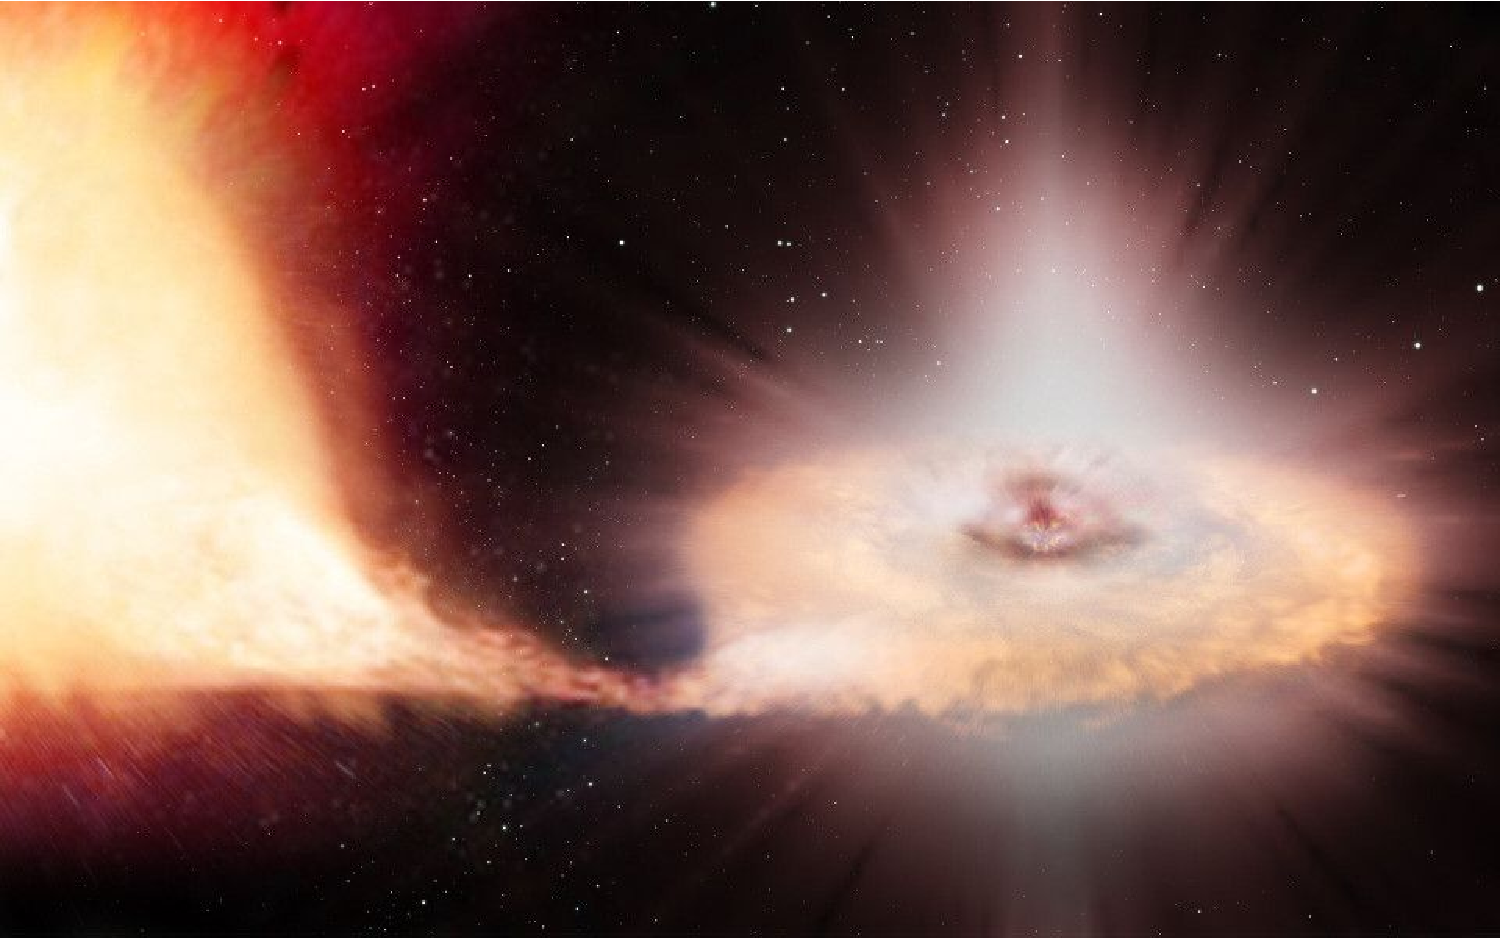
\includegraphics[width=0.7\textwidth]{figs/unit08_nova.pdf}\end{center}

As the white dwarf accumulates the matter emitted by its companion, its mass and its density steadily increase.
As the mass of the white dwarf approaches a value roughly 40\% larger than the mass of our sun, known as the \textit{Chandrasekhar limit} (named after \href{https://en.wikipedia.org/wiki/Subrahmanyan_Chandrasekhar}{Subrahmanyan Chandrasekhar}), its density becomes large enough for new types of nuclear fusion reactions to occur.
Instead of hydrogen or helium, which the white dwarf has already burned, these new fusion reactions involve carbon and oxygen, which remain present in abundance.
In just a few seconds, these fusion reactions run away, increase the temperature of the white dwarf to billions of kelvin, and blast it apart in a supernova explosion about five billion times brighter than the sun.

For obscure historical reasons, these particular stellar explosions are known as \textit{type-{\textrm I}a} (``one-A'') \textit{supernovas}.
The degeneracy pressure of low-temperature fermion gases plays a crucial role in these supernovas, by ensuring that a specific amount of mass has to build up in order to trigger the explosion.
The resulting regularity of type-{\textrm I}a supernovas allows them to be used as ``standard candles'' providing a consistent measure of astronomical distances.
This in turn enabled the discovery that the expansion of the universe is accelerating (a phenomenon popularly called `dark energy'), which was awarded the 2011 Nobel Prize in Physics.
% ------------------------------------------------------------------



% ------------------------------------------------------------------
\subsection{Relativistic ideal fermion gas}
Gases of relativistic fermions also play important roles in nature.
In fact, by changing units we can appreciate that the white dwarf Fermi energy discussed above, $E_F \sim 10^9~\text{K} \sim 0.3$~MeV is comparable to the $0.511$~MeV mass-energy of electrons, suggesting that relativistic effects may be non-negligible in white dwarfs. % eV~1.16^4 K is the Boltzmann constant
Such effects are indeed crucial to the computation of the Chandrasekhar limit mentioned above.

While full calculations for massive relativistic particles are beyond the scope of this module, we can take advantage of our earlier analyses of gases of massless photons to quickly obtain results for similar gases of massless fermions.
\textit{Neutrinos} (denoted `$\nu$') are physical examples of fermions whose masses are so small that they can be very well approximated as massless.
In fact, for many years neutrinos were thought to be exactly massless --- the discovery that neutrinos have non-zero masses was awarded the 2015 Nobel Prize in Physics.

In the same way as photons, massless fermions would travel at the speed of light, $c$, and have energies determined by their angular frequencies, $E_{\nu} = cp = \hbar \om$.
In a volume $V = L^3$, these energies are quantized as usual,
\begin{equation*}
  \om = \frac{2\pi c}{\la} = c \frac{\pi}{L} k,
\end{equation*}
where $k^2 = k_x^2 + k_y^2 + k_z^2$ and $k_{x, y, z} > 0$ are positive integers.
Just as for the non-relativistic case considered in \secref{sec:fermi_nonrel}, typical massless fermions, including neutrinos, have two degenerate energy levels for each distinct $\vec k$, with opposite spin.

The computations required to analyse a gas of massless fermions are very similar to the work we recently did for photon gases.
In particular, massless fermions are also easy to create and absorb, implying a vanishing chemical potential, $\mu \approx 0$.
Again approximating sums over discrete integer $k_{x, y, z}$ by integrals over continuous real $\khat_{x, y, z}$, and changing variables to integrate over the angular frequency, we end up with the grand-canonical potential
\begin{align}
  \Phi_{\nu} = -\frac{VT}{\pi^2 c^3} \int_0^{\infty} \om^2 \log\left[1 + e^{-\be \hbar \om}\right] \d{\om}. \label{eq:neutrino_grand}
\end{align}
The only changes here compared to \eq{eq:photon_grand} for the photon $\Phi_{\text{ph}}$ are a couple of negative signs, precisely as we would expect from comparing the Bose--Einstein and Fermi--Dirac grand-canonical potentials in \secref{sec:quantum_classical}.

Due to these negative signs, when we take derivatives of the potential to compute quantities like $\vev{E}_{\nu} = \pderiv{}{\be} \left[\be \Phi_{\nu}\right]$ and $\vev{N}_{\nu} = -\left. \pderiv{}{\mu} \Phi_{\nu}\right|_{\mu = 0}$, we will encounter slightly different but equally enjoyable integrals: % Fermi--Dirac integral involving polylog of -1 related to Dirichlet eta function...
\begin{align*}
  \int_0^{\infty} \frac{x^3}{e^x + 1} \d{x} & = \left(1 - \frac{1}{2^3}\right) \Gamma(4) \zeta(4) = \frac{7\pi^4}{120}, \\
  \int_0^{\infty} \frac{x^2}{e^x + 1} \d{x} & = \left(1 - \frac{1}{2^2}\right) \Gamma(3) \zeta(3) = \frac{3}{2} \zeta(3).
\end{align*}
Using these results, what are the average particle number and the average internal energy for a gas of massless fermions?
\begin{mdframed}
  \ \\[110 pt]
\end{mdframed}

You should again find $\vev{E}_{\nu} \propto \vev{N}_{\nu} T \propto VT^4$, and by noting that
\begin{equation*}
  \frac{\Phi_{\nu}}{T} = -\frac{V}{\pi^2 c^3} \left(\frac{T}{\hbar}\right)^3 \int_0^{\infty} x^2 \log\left[1 + e^{-x}\right] \d{x} \propto VT^3,
\end{equation*}
we can see that the entropy $S_{\nu} = \left(\vev{E}_{\nu} - \Phi_{\nu}\right) / T$ is constant when $V T^3 = \mbox{const}$.
Applying this, what is the pressure for a gas of massless fermions?
\begin{mdframed}
  \ \\[100 pt]
\end{mdframed}
You should find an equation of state with the usual functional form and just a new numerical factor:
\begin{equation*}
  P_{\nu} V = \frac{1}{3} \vev{E}_{\nu} = \frac{7\pi^4}{540\zeta(3)} \vev{N}_{\nu} T = \frac{(7/8)\zeta(4)}{(3/4)\zeta(3)} \vev{N}_{\nu} T \approx 1.05 \vev{N}_{\nu} T.
\end{equation*}
% ------------------------------------------------------------------



% ------------------------------------------------------------------
\subsection{\label{sec:Sommerfeld}Density of states \& Sommerfeld expansion}
In \eq{eq:fermi_E_N} we found that the average internal energy of a non-relativistic fermion gas becomes independent of the temperature in the limit $T \to 0$.
This means that its heat capacity,
\begin{equation*}
  c_v = \left. \pderiv{}{T} \vev{E} \right|_{N,V},
\end{equation*}
vanishes in this limit, which we could also see by considering the fluctuation--dissipation relation $c_v \propto \vev{\left(E - \vev{E}\right)^2}$ with only a single micro-state. % Again ignore irrelevant complication from possibility that only a portion of the degenerate energy levels at $E_F$ are filled

To derive the non-trivial heat capacity for a gas with a small but non-zero temperature, we need to move beyond approximating the Fermi function
\begin{equation*}
  F(E) = \frac{1}{e^{\be(E - \mu)} + 1}
\end{equation*}
as a step function, and return to the full \eq{eq:N_fermi} for the average particle number,
\begin{equation}
  \label{eq:number}
  \vev{N}_{\text{f}} = V \frac{\sqrt{2m^3}}{\pi^2 \hbar^3} \int_0^{\infty} F(E) \sqrt{E} \d{E} \equiv \int_0^{\infty} g(E) \; F(E) \d{E}.
\end{equation}
Here we have defined the \textbf{density of states}
\begin{equation*}
  g(E) \equiv V \frac{\sqrt{2m^3}}{\pi^2 \hbar^3} \sqrt{E} \equiv g_0 \; \sqrt{E}
\end{equation*}
as the number of energy levels per unit energy, each of which can hold at most a single fermion.
We can read \eq{eq:number} as saying that the total number of particles is given by integrating over the single-particle energy levels, $g(E)$, times the probability $F(E)$ that each of these energy levels is occupied.

The figures below, from Schroeder's \textit{Introduction to Thermal Physics}, illustrate this integral in the case of $T = 0$ (left) and $T > 0$ (right).
As we have already seen, when $T \to 0$ all energy levels with $E < E_F$ are occupied while all those with $E > E_F$ are unoccupied.
With $T > 0$, there is an exponentially suppressed probability for some energy levels with $E > E_F$ to be occupied.
Because the Fermi energy is set by the number of particles,
\begin{equation*}
  E_F = \frac{\hbar^2}{2m}\left(\frac{3\pi^2 \vev{N}_{\text{f}}}{V}\right)^{2 / 3},
\end{equation*}
having some of these particles occupy energy levels with $E > E_F$ requires that an equal number of energy levels with $E < E_F$ be unoccupied.

\noindent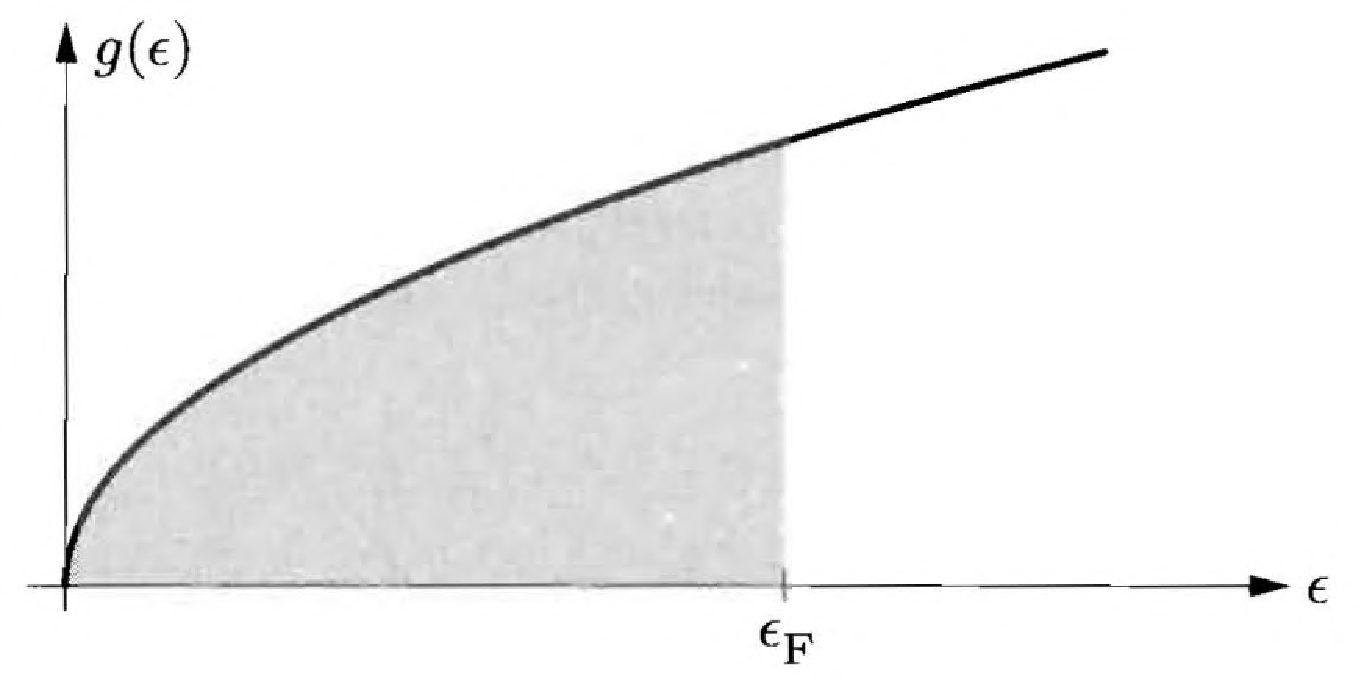
\includegraphics[width=0.45\textwidth]{figs/unit08_zero.pdf}\hfill 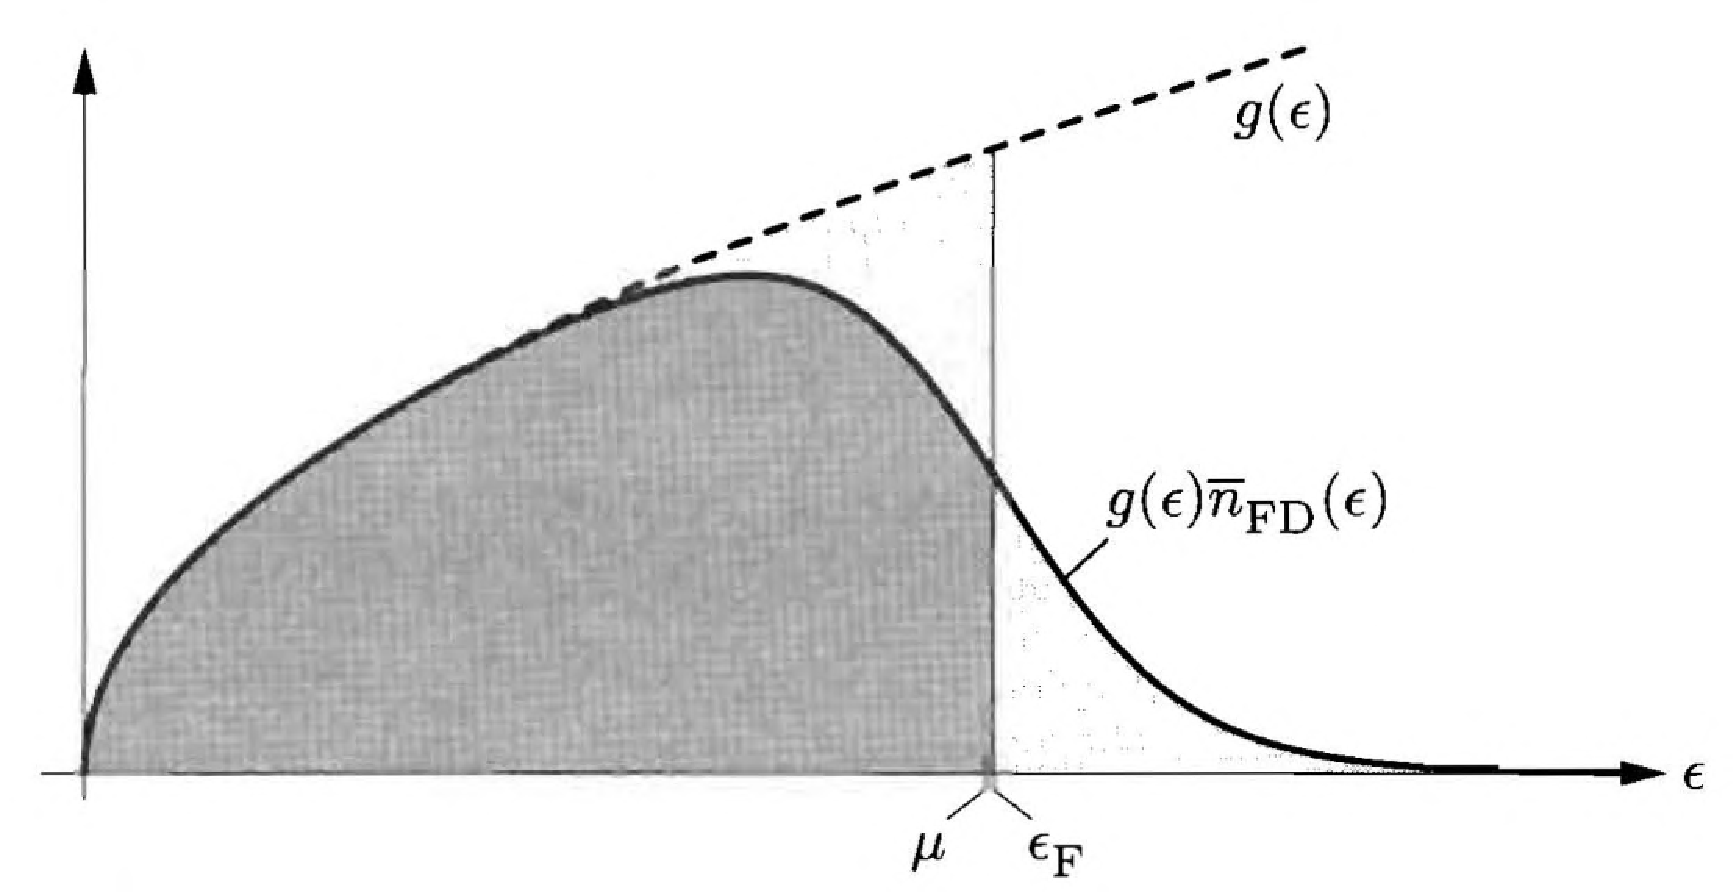
\includegraphics[width=0.45\textwidth]{figs/unit08_nonzero.pdf}

Note that $E = \mu$ is the point where the Fermi function $F(E) = \frac{1}{2}$.
We will see below that $\mu \leq E_F$, as shown in the right figure above, with equality when $T = 0$.

In order to determine the particle number and internal energy, we need to evaluate the integrals
\begin{align}
  \label{eq:DoS_full}
  \vev{N}_{\text{f}} & = g_0 \int_0^{\infty} F(E) \sqrt{E} \d{E} \qquad &
  \vev{E}_{\text{f}} & = g_0 \int_0^{\infty} E \; F(E) \sqrt{E} \d{E}
\end{align}
without approximating the Fermi function as a step function.
For $T \ll E_F$, we can do this through a \textbf{Sommerfeld expansion}.
Let's begin by considering the particle number.
The first step in the Sommerfeld expansion is integrating by parts:
\begin{mdframed}
  \ \\[120 pt]
\end{mdframed}

Changing variables to $x \equiv \be(E - \mu)$, you should find
\begin{equation*}
  \vev{N}_{\text{f}} = \frac{2}{3} g_0 \int_{-\be\mu}^{\infty} \frac{e^x}{\left(e^x + 1\right)^2} E^{3 / 2} \d{x}.
\end{equation*}
This is not obviously simpler than the expression we started with (especially because $E$ depends on $x$), but has the benefit of being exponentially suppressed for \textit{both}
\begin{align*}
                   x \gg 1  \qquad \Lra \qquad & \frac{e^x}{\left(e^x + 1\right)^2} \approx \frac{e^x}{e^{2x}} = \frac{1}{e^x} \\
  \mbox{and} \quad x \ll -1 \qquad \Lra \qquad & \frac{e^x}{\left(e^x + 1\right)^2} \approx \frac{e^x}{1} = \frac{1}{e^{-x}}.
\end{align*}
The additional $E^{3 / 2}$ factor is far too mild to overcome this exponential suppression.
In other words, non-negligible contributions to the integral as a whole come only from a region centered at $E = \mu$, which becomes narrower in $E$ as the temperature decreases (corresponding to larger $\be = 1 / T$).
This is illustrated by the plot below, which shows the exponential suppression setting in when $|E - \mu|$ is larger than a few times the temperature, and certainly for $|E - \mu| \gtrsim 5 / \be = 5T$. \\[-24 pt]
\begin{center}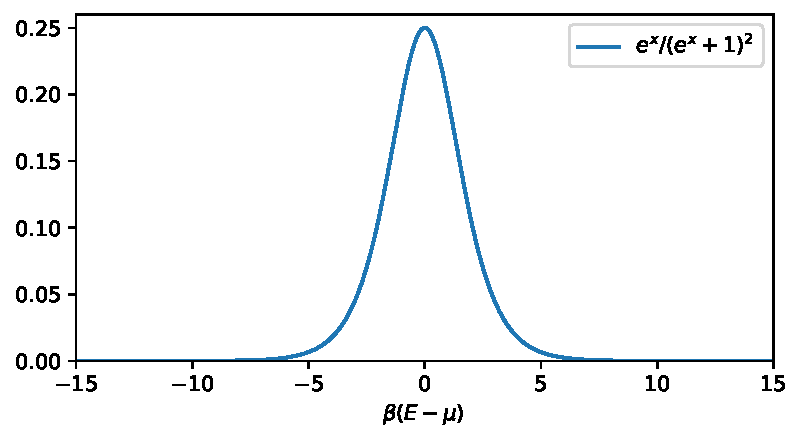
\includegraphics[width=0.7\textwidth]{figs/unit08_Sommerfeld.pdf}\end{center}

These considerations justify two low-temperature approximations.
First, recalling $\mu > 0$ at low temperatures, for large \be we are free to extend the lower limit of the integral to obtain a more convenient domain of integration,
\begin{equation*}
  \vev{N}_{\text{f}} = \frac{2}{3} g_0 \int_{-\be\mu}^{\infty} \frac{e^x}{\left(e^x + 1\right)^2} E^{3 / 2} \d{x} \approx \frac{2}{3} g_0 \int_{-\infty}^{\infty} \frac{e^x}{\left(e^x + 1\right)^2} E^{3 / 2} \d{x}.
\end{equation*}
Second, we can expand $E^{3 / 2}$ in a Taylor series around $E = \mu$, and truncate after the first few terms:
\begin{align*}
  E^{3 / 2} & \approx \mu^{3 / 2} + (E - \mu) \left. \pderiv{}{E} E^{3 / 2}\right|_{E = \mu} + \frac{1}{2} (E - \mu)^2 \left. \ppderiv{}{E} E^{3 / 2}\right|_{E = \mu} \\
            & = \mu^{3 / 2} + \frac{3}{2} (E - \mu) \mu^{1 / 2} + \frac{3}{8} (E - \mu)^2 \mu^{-1 / 2} = \mu^{3 / 2} + \frac{3}{2} \frac{x \mu^{1 / 2}}{\be} + \frac{3}{8} \frac{x^2 \mu^{-1 / 2}}{\be^2}.
\end{align*}

Switching to work with $T = 1 / \be$, the Sommerfeld expansion has given us a series of manageable integrals we can consider one by one:
\begin{equation*}
  \vev{N}_{\text{f}} \approx \frac{2}{3} g_0 \mu^{3 / 2} \cI_0 + g_0 T \mu^{1 / 2} \cI_1 + \frac{g_0 T^2}{4\mu^{1 / 2}} \cI_2.
\end{equation*}
\begin{mdframed}
  $\displaystyle \cI_0 = \int_{-\infty}^{\infty} \frac{e^x}{\left(e^x + 1\right)^2} \d{x} = $ \\[70 pt]
  $\displaystyle \cI_1 = \int_{-\infty}^{\infty} \frac{x e^x}{\left(e^x + 1\right)^2} \d{x} = $ \\[70 pt]
  $\displaystyle \cI_2 = \int_{-\infty}^{\infty} \frac{x^2 e^x}{\left(e^x + 1\right)^2} \d{x} = $ \\[70 pt]
\end{mdframed}
Collecting the results and restoring $g_0 = V \frac{\sqrt{2m^3}}{\pi^2 \hbar^3}$, you should find
\begin{equation*}
  \vev{N}_{\text{f}} \approx \frac{2}{3} g_0 \mu^{3 / 2} + g_0 \frac{\pi^2 T^2}{12\mu^{1 / 2}} = V \frac{(2m\mu)^{3 / 2}}{3\pi^2\hbar^3} + V \frac{\sqrt{2m^3}}{12\hbar^3 \mu^{1 / 2}} T^2.
\end{equation*}
The first term reproduces what we found with the step-function approximation in \secref{sec:fermi_lowT}, while the second term provides the promised leading-order temperature dependence in the Sommerfeld expansion.
This becomes more interesting if we rearrange \eq{eq:Fermi_energy} to work in terms of the Fermi energy:
\begin{mdframed}
  \ \\[100 pt]
\end{mdframed}

The result
\begin{equation*}
  \frac{\mu}{E_F} \approx \left[1 - \frac{\pi^2 T^2}{8 E_F^{3 / 2} \mu^{1 / 2}}\right]^{2 / 3}
\end{equation*}
can be simplified through one final low-temperature approximation.
Because $T$ is small, just in the second term above we can set $E_F \approx \mu$ (the zero-temperature relation).
Then
\begin{equation}
  \label{eq:mu_vs_T}
  \frac{\mu}{E_F} \approx 1 - \frac{\pi^2 T^2}{12 E_F^2},
\end{equation}
which confirms our earlier claim $\mu \leq E_F$, and reveals that the leading correction to the zero-temperature relation is quadratic in $\frac{T}{E_F} \ll 1$.

The calculation is essentially the same for the internal energy from \eq{eq:DoS_full}.
With $E^{3 / 2}$ in place of $E^{1 / 2}$, integrating by parts just gives
\begin{equation*}
  \vev{E}_{\text{f}} = g_0 \int_0^{\infty} \frac{E^{3 / 2}}{e^{\be(E - \mu)} + 1} \d{E} \approx \frac{2}{5} g_0 \int_{-\infty}^{\infty} \frac{e^x}{\left(e^x + 1\right)^2} E^{5 / 2} \d{x}
\end{equation*}
with the same $x = \be(E - \mu)$ and extended limit of integration.
The Taylor expansion
\begin{equation*}
  E^{5 / 2} \approx \mu^{5 / 2} + \frac{5}{2} (E - \mu) \mu^{3 / 2} + \frac{15}{8} (E - \mu)^2 \mu^{1 / 2} = \mu^{5 / 2} + \frac{5}{2} \frac{x \mu^{3 / 2}}{\be} + \frac{15}{8} \frac{x^2 \mu^{1 / 2}}{\be^2}
\end{equation*}
also produces the same integrals, with different coefficients:
\begin{equation*}
  \vev{E}_{\text{f}} \approx \frac{2}{5} g_0 \mu^{5 / 2} \cI_0 + g_0 T \mu^{3 / 2} \cI_1 + \frac{3}{4} g_0 T^2 \mu^{1 / 2} \cI_2 = \frac{2}{5} g_0 \mu^{5 / 2} + \frac{1}{4} g_0 \pi^2 T^2 \mu^{1 / 2}.
\end{equation*}
Inserting $g_0 = \frac{3\vev{N}_{\text{f}}}{2E_F^{3 / 2}}$, we have
\begin{equation*}
  \vev{E}_{\text{f}} \approx \frac{3}{5} \vev{N}_{\text{f}} \frac{\mu^{5 / 2}}{E_F^{3 / 2}} + \frac{3}{8} \vev{N}_{\text{f}} \pi^2 T^2 \frac{\mu^{1 / 2}}{E_F^{3 / 2}},
\end{equation*}
which we can simplify by applying \eq{eq:mu_vs_T} and dropping $\cO\left(T^3\right)$ terms:
\begin{mdframed}
  \ \\[100 pt]
\end{mdframed}
From your result you should obtain the heat capacity
\begin{equation*}
  c_v = \left. \pderiv{}{T} \vev{E} \right|_{N,V} \approx \frac{\pi^2}{2} \frac{\vev{N}_{\text{f}}}{E_F} T.
\end{equation*}
This low-temperature linear dependence on $T$ agrees with experimental heat capacity measurements, as we have seen in tutorials.

As a final comment in this section, let's consider what would happen to $\vev{N}_{\text{f}}$ at higher temperatures $T^2 \sim E_F^2$, for which the two terms in \eq{eq:mu_vs_T} would cancel out, leaving $\cO(T^4 / E_F^4)$ effects non-negligible.
In this regime, there's no guarantee that the low-temperature Sommerfeld expansion would even converge, so we need to work with the full integral from \eq{eq:DoS_full}.
Fortunately, it is not hard to numerically evaluate this integral, which is done by \href{https://github.com/daschaich/MATH327_2025/blob/main/lecture_notes/unit08_fermi-gas.py}{this Python code}.
For the purpose of numerical analysis, it's best to express everything in terms of dimensionless ratios, such as
\begin{align*}
  t & \equiv \frac{T}{E_F} \qquad &
  c & \equiv \frac{\mu}{E_F} \qquad &
  x & \equiv \frac{E}{T} = \be E.
\end{align*}
Also inserting $g_0 = \frac{3\vev{N}_{\text{f}}}{2E_F^{3 / 2}}$, we have
\begin{equation*}
  \vev{N}_{\text{f}} = \frac{3\vev{N}_{\text{f}}}{2E_F^{3 / 2}} \int_0^{\infty} \frac{\sqrt{E}}{e^{\be(E - \mu)} + 1} dE = \frac{3\vev{N}_{\text{f}}}{2} t^{3 / 2} \int_0^{\infty} \frac{\sqrt{x} e^{-x}}{e^{-c / t} + e^{-x}} \d{x},
\end{equation*}
working with small $e^{-\be E} = e^{-x}$ rather than large $e^x$ to avoid numerical overflow.

As in \eq{eq:mu_vs_T}, $\vev{N}_{\text{f}}$ drops out, and we end up with the consistency condition
\begin{equation}
  1 = \frac{3}{2} t^{3 / 2} \int_0^{\infty} \frac{\sqrt{x} e^{-x}}{e^{-c / t} + e^{-x}} \d{x}.
\end{equation}
If we fix the temperature $t = T / E_F$ in units of the Fermi energy, by numerically evaluating this integral with different values of $c = \mu / E_F$ we can determine the self-consistent value of the chemical potential, also in units of the Fermi energy.
The red $\times$'s in the figure below are results of such work for eleven temperatures $0.1 \leq t \leq 2$, compared to the $\cO\!\left(t^2\right)$ result from the Sommerfeld expansion, \eq{eq:mu_vs_T}.
This leading-order Sommerfeld expansion clearly deviates from the full results by the time $T \sim E_F$.
The more interesting result is that the chemical potential continues to decrease as the temperature increases, becoming negative for $T \gtrsim E_F$ and approaching the expected high-temperature classical limit.

\begin{center}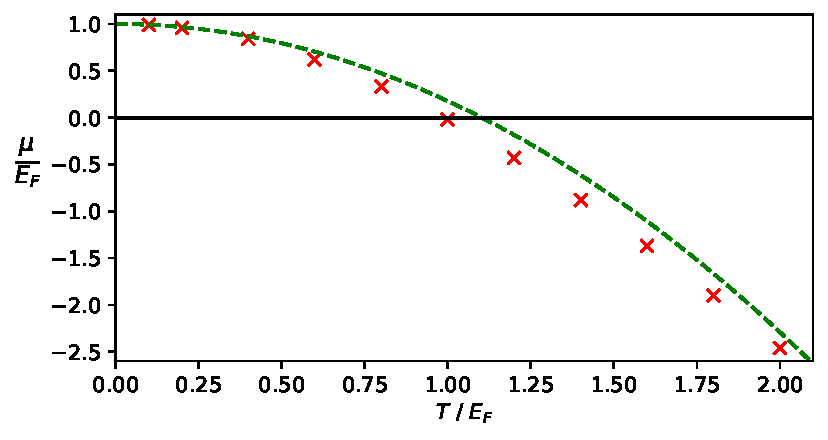
\includegraphics[width=0.8\textwidth]{figs/unit08_fermi-gas.pdf}\end{center}
% ------------------------------------------------------------------


\newpage
% ------------------------------------------------------------------
\renewcommand{\thisunit}{MATH327 Unit 9}
\renewcommand{\moddate}{Last modified 1 May~2025}
\setcounter{section}{9}
\setcounter{subsection}{0}
\phantomsection
\addcontentsline{toc}{section}{Unit 9: Interacting systems}
\section*{Unit 9: Interacting systems}
\subsection{\label{sec:Ising}The Ising model}
So far in this module we have considered `ideal' systems whose degrees of freedom do not interact with each other.
While we have seen that statistical mechanics employing this approximation of non-interacting particles can provide excellent descriptions of real physical systems ranging from the low-temperature heat capacities of solids to solar radiation and the cosmic microwave background, there are crucial emergent phenomena that this approach fails to predict.

An important class of examples, which we investigate in this unit, are \textit{phase transitions}.
These occur when interactions allow extremely different large-scale behaviours to arise from the same set of degrees of freedom, depending on control parameters such as the temperature or pressure.
Phase transitions occur in both everyday and extreme situations.
Everyday examples include the liquid--gas transition of H$_2$O molecules from water to steam upon boiling a kettle, as well as the transition from liquid water to solid ice as the temperature decreases.
In the extreme conditions following the big bang, matter in the universe existed as a charged plasma of quarks and gluons.
Once the universe was a few micro-seconds old, it cooled enough for this matter to transition into the protons and neutrons we are made out of today. % Strictly speaking, this was almost certainly a crossover rather than a true phase transition...

An intermediate example in between the everyday and the extreme involves two layers of graphene as illustrated in the figure below.\footnote{Heather M. Hill, ``\href{https://doi.org/10.1063/PT.3.4384}{Twisted bilayer graphene enters a new phase}'', \textit{Physics Today} \textbf{73}:18, 2020.}
Graphene is an amazing material (recognized by the 2010 Nobel Prize in Physics) that consists of a single-atom-thick sheet of carbon atoms arranged in a hexagonal `honeycomb' lattice.
Under most conditions, graphene is an electrical insulator.
However, if two graphene sheets are stacked and rotated with respect to each other by a small ``magic angle'' $\theta \approx 1.1^{\circ}$, the system transitions into a superconducting phase at low temperatures $T \lesssim 1.7$~K.
Superconductivity allows electrical current to flow with no resistance, meaning that no energy is lost to the production of waste heat.
If we could discover or design materials that exhibit superconductivity at everyday temperatures $T \sim 300$~K rather than low $T \sim \cO(1)$~K, it would revolutionize the energy efficiency of electronics and the power grid.

\begin{center}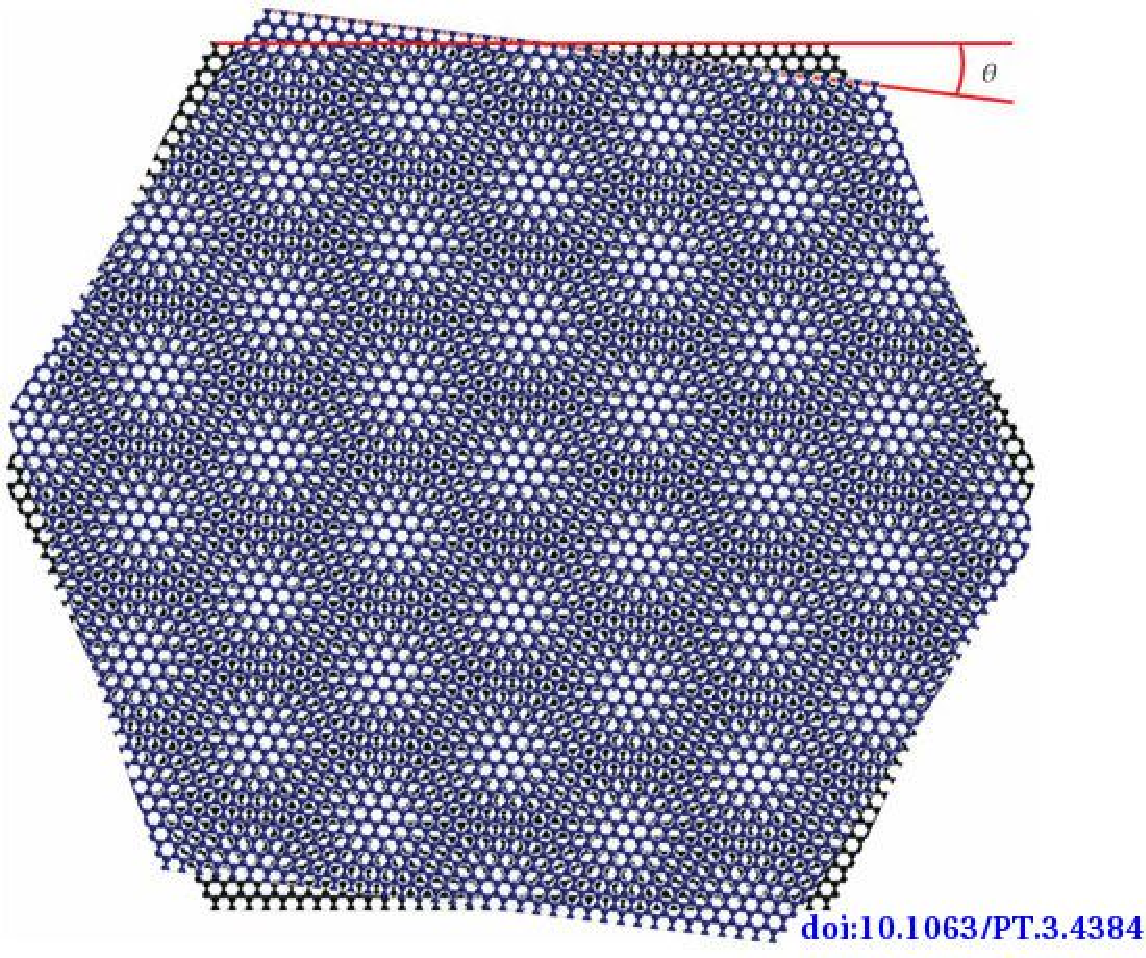
\includegraphics[width=0.475\textwidth]{figs/unit09_graphene.pdf}\end{center}

With this motivation for investigating phase transitions, let's step back to introduce interactions and explore their effects using simple spin systems of the sort we considered in units $2$ and $3$.
In the non-interacting case we previously analysed (\eq{eq:spin_energy}), the internal energy of the system is
\begin{equation*}
  E_i = -H \sum_{n = 1}^N s_n \qquad \mbox{(non-interacting)}
\end{equation*}
for micro-state $\om_i$ specified by the $N$ spins $\left\{s_n\right\}$ (and, as always for this module, in thermodynamic equilibrium).
Here $H > 0$ is the constant strength of an external magnetic field and the orientation of the $n$th spin, $s_n$, takes one of only two possible values: $s_n = 1$ if the spin is aligned parallel to the field and $s_n = -1$ if the spin is aligned anti-parallel to the field.
The ground state of the system features all $N$ spins aligned parallel to the magnetic field, with minimal energy $E_0 = -NH$.

In this unit we will only consider systems of distinguishable spins that we label by their fixed position in a $d$-dimensional simple cubic \textbf{lattice}.
The $d = 1$ case of a one-dimensional lattice is precisely the system of spins arranged in a line that we analysed in \secref{sec:spin_chain}.
This and the case of $d = 2$ are both easy to visualize and draw on a sheet of paper:
\begin{mdframed}
  \ \\[100 pt]
\end{mdframed}
While we can only have physical lattices with $d = 1$, $2$ or $3$ in nature, the mathematical construction works just as well for any integer $d \geq 1$.

We can see that the total internal energy of the non-interacting system can easily be written as a sum over energies $\eps_n$ for each individual spin,
\begin{align*}
  \eps_n & = -H s_n &
  E_i & = \sum_{n = 1}^N \eps_n \qquad \mbox{(non-interacting)}.
\end{align*}
This is a generic feature of non-interacting systems, and an aspect of the \textbf{factorization} that enormously simplifies calculations --- in this case by causing the $N$-particle partition function (\eq{eq:spin_part_func}) to take the form of a product of $N$ identical terms, $Z_N = \left[2\cosh\left(\be H\right)\right]^N = Z_1^N$.
However, it is possible to have non-factorizable systems in which the internal energy can be expressed as a sum of this sort.
A stronger condition needs to be satisfied in order to guarantee factorization, and this conditions rigorously defines what it means for a system to be non-interacting.

\begin{shaded}
  Let $\De E_j$ be the change in the system's internal energy caused by changing its $j$th degree of freedom.
  Then the system is defined to be \textbf{non-interacting} if and only if $\De E_j$ is independent of all other degrees of freedom $k \ne j$. % for an arbitrary $j$...
\end{shaded}

For our system of $N$ distinguishable spins, the only possible change we can make to a degree of freedom is to negate it, $s_j \to -s_j$, which corresponds to flipping its alignment relative to the external magnetic field.
It is easy to check that the change in the internal energy resulting from such a spin flip satisfies our definition of a non-interacting system:
\begin{mdframed}
  \ \\[80 pt]
\end{mdframed}

Now let's make things more interesting by considering a different spin system that includes a simple two-spin contribution to the internal energy:
\begin{equation}
  \label{eq:Ising_energy}
  E_i = -\sum_{(jk)} s_j s_k - H \sum_{n = 1}^N s_n.
\end{equation}
The first sum runs over all pairs of nearest-neighbour spins in the lattice, denoted $(jk)$.
What is the change in energy $\De E_j$ from \eq{eq:Ising_energy} upon negating $s_j \to -s_j$?
Does this indicate an interacting or non-interacting system?
\begin{mdframed}
  \ \\[100 pt]
\end{mdframed}

The pictures on the next page illustrate nearest-neighbour pairs for simple cubic lattices in $d = 2$ and $3$ dimensions, while also introducing some additional lattice terminology.
Instead of drawing up- and down-pointing arrows, these pictures identify the spins with \textit{sites} in the lattice represented as points (or larger filled circles).
In simple cubic lattices, all sites are positioned in a regular grid, separated by a constant distance along each basis vector.
We can also draw \textit{links} as solid lines connecting these nearest-neighbour sites, with each link corresponding to a term in $\sum_{(jk)}$.
The picture of a two-dimensional lattice on the left highlights the four links (with red hatch marks) that correspond to the four nearest neighbours (circled in red) of a particular site (circled in blue).
For $d \geq 2$, the elementary unit of surface area is called a \textit{plaquette}, while for $d \geq 3$ the elementary unit of volume is called a \textit{cube}.

\begin{center}
  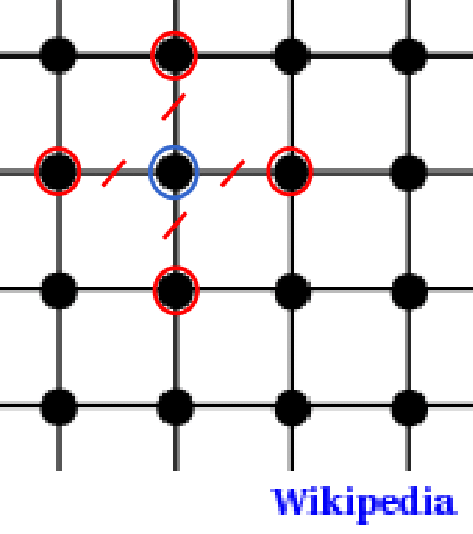
\includegraphics[height=0.4\textwidth]{figs/unit09_lattice_2d.pdf}\hfill
  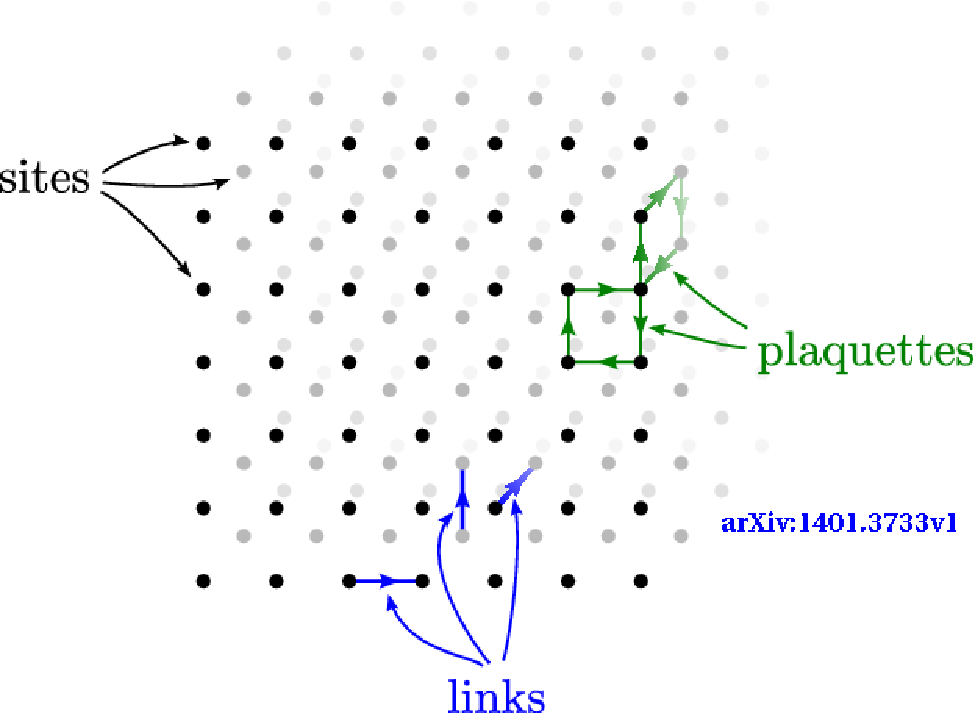
\includegraphics[height=0.4\textwidth]{figs/unit09_lattice_3d.pdf}
\end{center}

The nearest-neighbour pairs appearing in the energy, \eq{eq:Ising_energy}, correspond to the links in the lattice, $\ell = (jk)$.
Assuming a finite lattice, the presence of any edges will make analyses more complicated, since sites on the edges or in the corners will have a different number of nearest neighbours than other sites.
We can avoid this complication by imposing \textbf{periodic boundary conditions}, which remove these edges by adding links between each site on the left edge of the lattice and the corresponding site on the right edge, and similarly in all other dimensions.
This is illustrated below for the simple case of the one-dimensional lattice, drawn as a circle to emphasize that all $N$ sites remain separated by a constant distance.
In higher dimensions, periodic boundary conditions produce flat (zero-curvature) $d$-dimensional tori that preserve the simple cubic lattice structure. \\[-24 pt]
\begin{center}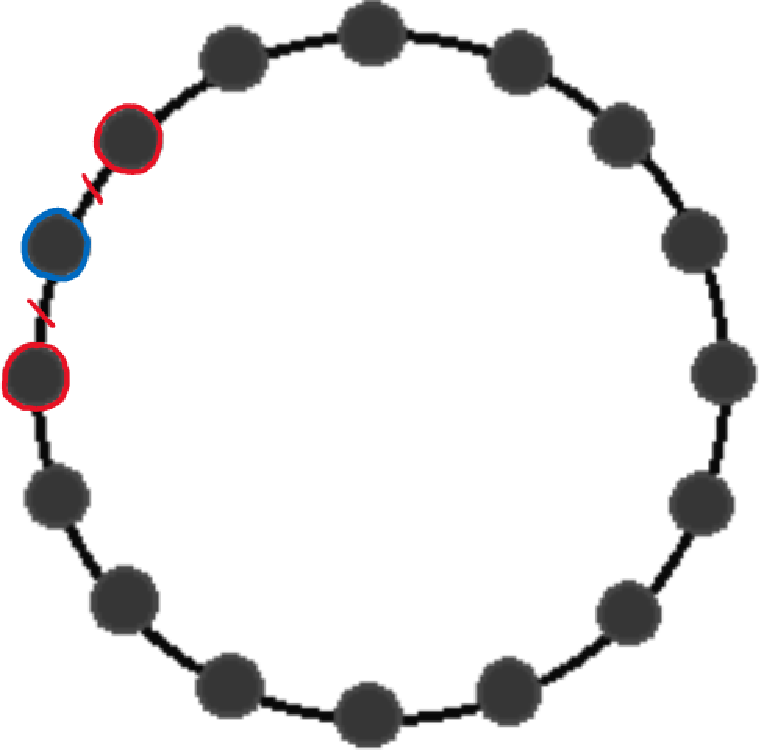
\includegraphics[width=0.4\textwidth]{figs/unit09_lattice_1d.pdf}\end{center}

Periodic boundary conditions cause the one-dimensional lattice drawn above to have the same number of links as sites:
Each site has two links connecting it to its two nearest neighbours, and each of those links is shared between two sites, so that $\#\ell = 2N / 2 = N$.
Looking back to the two-dimensional lattice drawn farther above, the four links per site produce $\#\ell = 4N / 2 = 2N$.
How many terms are there in the sum $\sum_{(jk)}$ in \eq{eq:Ising_energy} for $N$-site lattices with periodic boundary conditions in $d$ dimensions?
\begin{mdframed}
  \ \\[50 pt]
\end{mdframed}

The energy of interacting spins given by \eq{eq:Ising_energy}, with a lattice structure specifying which spins form the nearest-neighbour pairs $(jk)$, defines a famous system known as the $d$-dimensional \textbf{Ising model}.
Since the 1960s, the Ising model has been the basis of thousands of scientific studies analysing everything from ferromagnetism to neural networks to urban segregation.\footnote{For a brief discussion, see Charlie Wood, ``\href{https://www.quantamagazine.org/the-cartoon-picture-of-magnets-that-has-transformed-science-20200624/}{The Cartoon Picture of Magnets That Has Transformed Science}'', \textit{Quanta Magazine}, 2020.}
The model was proposed in 1920 by \href{https://en.wikipedia.org/wiki/Wilhelm_Lenz}{Wilhelm Lenz}, whose PhD student \href{https://en.wikipedia.org/wiki/Ernst_Ising}{Ernst Ising} solved the one-dimensional system for his thesis in 1924.
Exactly solving the two-dimensional case (with $H = 0$) took another twenty years, culminating in renowned work by \href{https://en.wikipedia.org/wiki/Lars_Onsager}{Lars Onsager} in 1944.
The three-dimensional Ising model remains an open mathematical question, with no known exact solution.

In this context, `solving' the Ising model means deriving a closed-form expression for its canonical partition function,
\begin{equation*}
  Z(\be, N, H) = \sum_{\left\{s_n\right\}} \exp\left[-\be E(s_n)\right] = \sum_{\left\{s_n\right\}} \exp\left[\be\sum_{(jk)} s_j s_k + \be H \sum_n s_n\right].
\end{equation*}
As in \secref{sec:spin_info}, the partition function sums over all possible spin configurations $\left\{s_n\right\}$, which amounts to a sum of $2^N$ exponential factors for $N$ spins, with $\cO(N)$ terms within each exponential.
Now that the system is interacting, the partition function no longer factorizes into the $N$ identical $\cosh$ factors of \eq{eq:spin_part_func}, making it extremely difficult to evaluate.
This is why there is no known exact solution for the three-dimensional Ising model, and it also makes `brute-force' numerical computations impractical.
Even for a system of $N = 1023$ spins, twenty orders of magnitude smaller than our typical $N \sim 10^{23}$, there are roughly $2^{1023} \sim 10^{310}$ terms in the partition function, far beyond the capabilities of existing or foreseeable supercomputers.
% ------------------------------------------------------------------



% ------------------------------------------------------------------
\subsection{\label{sec:Ising_phases}Ising model phases and phase transition}
Even without exactly solving the Ising model, we can still make robust predictions for its large-scale behaviour by considering the simplified limits of high and low temperature, much as we did for non-interacting spin systems in \secref{sec:spin_info}.
We can also simplify the system by setting $H = 0$ in this section, and considering just
\begin{align}
  \label{eq:Ising_zero_field}
  E_i & = -\sum_{(jk)} s_j s_k &
  Z(\be, N) & = \sum_{\left\{s_n\right\}} \exp\left[\be\sum_{(jk)} s_j s_k\right].
\end{align}
We will see that the behaviour of this zero-field Ising model is qualitatively different at high temperatures compared to low temperatures.
In other words, the system exhibits at least two distinct phases for different temperatures.
This is a necessary but not sufficient condition for there to be a true phase transition --- it leaves open the possibility of a gradual \textit{crossover} between these two phases, as opposed to a rapid transition.
In this section we will use the Ising model to more rigorously define what exactly constitutes a phase transition, and how this can be distinguished from a crossover.

First, though, let's consider the \textbf{high-temperature} limit $\be \to 0$, where the Ising model partition function becomes extremely simple:
\begin{mdframed}
  \ \\[40 pt]
\end{mdframed}
In this limit, all $2^N$ spin configurations are adopted with the same probability $p_i = 1 / 2^N$, regardless of their internal energy from \eq{eq:Ising_zero_field}.
In effect, that energy has become negligible compared to the temperature.

There is a simple observable we can use to characterize this high-temperature phase.
This is the \textbf{magnetization} $M = n_+ - n_-$, retaining our definition of $n_{\pm}$ as the number of spins with value $\pm 1$, even without an external field for them to align with or align against.
It is convenient to normalize the magnetization by the number of spins,
\begin{equation}
  \label{eq:Ising_magnet}
  m \equiv \frac{M}{N} = \frac{n_+ - n_-}{n_+ + n_-},
\end{equation}
so that $-1 \leq m \leq 1$ for any value of $N$.
In addition, without an external field to distinguish between $\pm 1$ spins, it is also convenient to consider the absolute magnitude $0 \leq |m| \leq 1$.

Our task is now to determine the expectation value of the magnetization at high temperatures.
Above we found that all spin configurations are equally probable in this regime, so $\vev{|m|}$ will be determined by how many of these equally probable micro-states have a particular magnetization.
For example, there are only two micro-states with $|m| = 1$, corresponding to $(n_+, n_-) = (N, 0)$ and $(0, N)$.
In general, just as we saw in \eq{eq:spin_states}, there are
\begin{equation*}
  \binom{N}{n_+} = \binom{N}{n_-} = \frac{N!}{n_+! \; n_-!}
\end{equation*}
equally probable micro-states with a given $n_+ = N - n_-$.
For large $N \gg 1$ this binomial coefficient has a factorially narrow peak around
\begin{equation*}
  n_+ = n_- = \frac{1}{2} N \qquad \lra \qquad |m| = 0.
\end{equation*}
This characterizes a \textbf{disordered phase} with similar numbers of up- and down-pointing spins producing a small magnetization.
In the \textit{thermodynamic limit} $N \to \infty$, the expectation value of the magnetization in the disordered phase vanishes exactly, $\vev{|m|} \to 0$.

We next need to determine $\vev{|m|}$ in the \textbf{low-temperature} limit $\be \to \infty$.
In this regime, as we saw in \secref{sec:spin_chain}, the Boltzmann factor $\exp\left[\be\sum_{(jk)} s_j s_k\right]$ makes it exponentially more likely for the system to adopt micro-states with lower energies.
In particular, we can expect the ground state to dominate the expectation value of the magnetization, $\vev{|m|}$, up to exponentially suppressed corrections from excited states.
With $H = 0$, the Ising model has two degenerate ground states corresponding to the two ways all the spins can be aligned with each other: $(n_+, n_-) = (N, 0)$ and $(0, N)$.
What is the ground-state energy of the $N$-site Ising model in $d$ dimensions?
\begin{mdframed}
  \ \\[50 pt]
\end{mdframed}

As mentioned above, both of these degenerate ground states have the maximal magnetization $|m| = 1$.
Let's check what effect the first excited state would have on the overall magnetization of the system.
For $d > 1$, the first excited energy level is obtained by flipping a single spin, negating its value.
Starting from the two degenerate ground states, this produces all possible micro-states with $(n_+, n_-) = (N - 1, 1)$ and $(1, N - 1)$.
Because any one of the $N$ spins in the lattice could be flipped, the degeneracy of this first excited energy level grows with $N$:
\begin{equation*}
  \binom{N}{1} + \binom{N}{N - 1} = 2N.
\end{equation*}
At the same time, as $N$ increases the magnetization of each of these micro-states gets closer to that of the ground state,
\begin{equation*}
  |m| = \frac{N - 2}{N} = 1 - \frac{2}{N}.
\end{equation*}
The key factor is the probability for the system to be in one of these micro-states, which depends on the value of the energy $E_1$ for the first excited energy level.
What is this $E_1$ for the $N$-site Ising model in $d$ dimensions?
\begin{mdframed}
  \ \\[75 pt]
\end{mdframed}

Let's bring everything together by computing the relative probability for the $d$-dimensional Ising model to be in its ground state with $|m| = 1$ compared to its first excited state with $|m| = 1 - \frac{2}{N}$.
We just need to multiply the degeneracy of each energy level times the corresponding Boltzmann factor, while the $\frac{1}{Z}$ normalization cancels out in the ratio
\begin{equation*}
  \frac{P(E_0)}{P(E_1)} = \frac{2\cdot \exp\left[\be d\cdot N\right]}{2N\cdot \exp\left[\be \left(d\cdot N - 4d\right)\right]} = \frac{\exp\left[4\be d\right]}{N}.
\end{equation*}
For any fixed $N$, a sufficiently low temperature will cause the ground state to dominate, with exponentially suppressed contributions from higher energy levels, just as we previously found for simpler non-interacting systems.
This characterizes an \textbf{ordered phase} with essentially all spins aligned in the same direction, producing a large expectation value for the magnetization, $\vev{|m|} \to 1$.

We have now seen how the behaviour of the magnetization $\vev{|m|}$ distinguishes the high- and low-temperature phases of the zero-field Ising model in $d > 1$ dimensions.
In the high-temperature disordered phase, the magnetization is small and $\vev{|m|} \to 0$ in the thermodynamic limit $N \to \infty$.
In the low-temperature ordered phase, the magnetization is large and $\vev{|m|} \to 1$ as $T \to 0$.

This contrast between ordered and disordered phases is typical behaviour for interacting statistical systems.
These two phases are distinguished by an \textbf{order parameter} --- an observable (related to a derivative of the free energy) that is zero in the disordered phase but non-zero in the ordered phase.\footnote{There are atypical (but interesting and important) \textit{topological phase transitions} that are not characterized by such an order parameter.  The most famous example is the BKT phase transition named after \href{https://en.wikipedia.org/wiki/Vadim_Berezinskii}{Vadim Berezinskii}, \href{https://en.wikipedia.org/wiki/J._Michael_Kosterlitz}{J.\ Michael Kosterlitz} and \href{https://en.wikipedia.org/wiki/David_J._Thouless}{David Thouless}, which was recognized by the 2016 Nobel Prize in Physics.  It is also possible for a single system to have multiple distinct phase transitions, each characterized by a different order parameter.}
The magnetization is the order parameter for the Ising model, and we will relate it to the free energy in the next section.
Note that the order parameter need not reach its maximum value in the ordered phase --- it only needs to be non-zero.
The details of how the order parameter changes between zero and non-zero values distinguish crossovers from true transitions.

\begin{shaded}
  A \textbf{phase transition} is defined by a discontinuity or divergence in the order parameter or its derivative(s), in the $N \to \infty$ thermodynamic limit.
  The value(s) of the control parameter(s) at which the discontinuity occurs define the \textit{critical point} corresponding to the transition.
\end{shaded}

For the zero-field Ising model, since we have set $H = 0$, the only remaining control parameter is the temperature $T$.
Any phase transition would therefore occur at a \textbf{critical temperature} $T_C$.
The sketches on the next page illustrate the most common types of phase transitions.
When the order parameter (OP) itself is discontinuous (shown by a dashed line), the transition is said to be a \textit{first-order} phase transition. % TODO: Leads to non-zero latent heat...
When the order parameter is continuous at $T_C$ but its first derivative with respect to the control parameter is discontinuous (typically divergent), the transition is said to be a \textit{second-order} phase transition.
Historically, this naming scheme was extended to $n$th-order phase transitions for which discontinuities don't occur until the $(n-1)$th derivative of the order parameter (related to an $n$th derivative of the free energy).
At present it is more common for any phase transition with a continuous order parameter to be called simply a second-order transition.

\begin{center}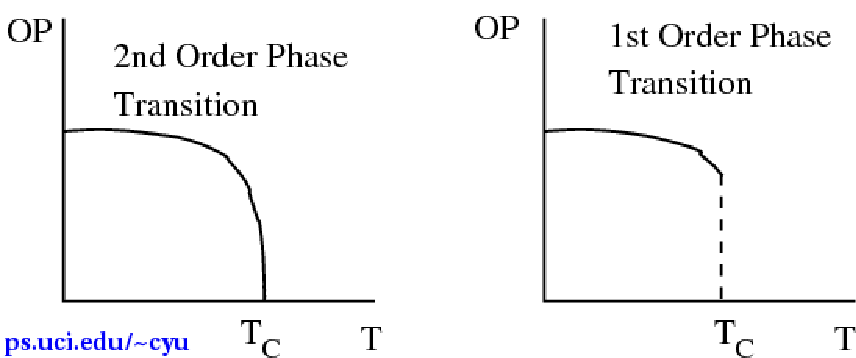
\includegraphics[width=\textwidth]{figs/unit09_transitions.pdf}\end{center}

In practice, any system with a finite number of degrees of freedom will not exhibit a true discontinuity or divergence in any observable.
As a result, it is sometimes said that true phase transitions only occur in the $N \to \infty$ thermodynamic limit, but I consider this excessively pedantic, especially given the finite number of atoms in the observable universe.
We are still able to distinguish crossovers from true phase transitions when considering a finite number of degrees of freedom, by analysing the way in which the system approaches the thermodynomic limit.
If there is time and interest, we can explore such \textit{finite-size scaling}, but first we will develop a useful approximation technique, and apply it to the Ising model to investigate its (dimensionality-dependent) phase transition in more detail.
% ------------------------------------------------------------------



% ------------------------------------------------------------------
\subsection{\label{sec:mean_field}The mean-field approximation}
Having identified the low-temperature ordered phase and high-temperature disordered phase of the zero-field Ising model, let's now restore a non-zero external magnetic field, $H > 0$.
This will allow us to gain a deeper appreciation of the magnetization (now with no absolute value) by noting that \eq{eq:Ising_magnet} means it is just the average spin:
\begin{equation*}
  m = \frac{M}{N} = \frac{1}{N}\left(n_+ - n_-\right) = \frac{1}{N} \sum_{n = 1}^N s_n.
\end{equation*}
We can benefit from this observation in two ways.
First, we can recognize the magnetization in the internal energy of the full Ising model with $H >0$:
\begin{equation*}
  E_i = -\sum_{(jk)} s_j s_k - H \sum_{n = 1}^N s_n = -\sum_{(jk)} s_j s_k - H N m = -\sum_{(jk)} s_j s_k - H M.
\end{equation*}
The corresponding canonical partition function is
\begin{equation*}
  Z = \sum_{\left\{s_n\right\}} \exp\left[\be \sum_{(jk)} s_j s_k + \be H M\right].
\end{equation*}
\newpage
\noindent Based on this expression, and our earlier experience with the entropy and internal energy, we can anticipate that $\vev{m} = \vev{M} / N$ is related to the derivative of the Helmholtz free energy $F = -T\log Z$ with respect to the field strength $H$:
\begin{mdframed}
  \ \\[100 pt]
\end{mdframed}
As promised in the previous section, this relation ensures that the magnetization is an appropriate order parameter for the Ising model phase transition.

The second way we can benefit from relating the magnetization to the average spin is to express the Ising model in terms of the expectation value
\begin{equation*}
  \vev{m} = \frac{1}{Z} \sum_{\left\{s_n\right\}} m \; e^{-\be E(s_n)} = \frac{1}{N} \sum_{n = 1}^N \vev{s_n}.
\end{equation*}
The expectation value of the average spin, $\frac{1}{N} \sum_{n = 1}^N \vev{s_n}$, is independent of the spin configuration $\left\{s_n\right\}$ and is simply a function of the inverse temperature \be and magnetic field strength $H$.
By adding and subtracting factors of $\vev{m}$, we can exactly rewrite each nearest-neighbour term in the Ising model energy, \eq{eq:Ising_energy}, as
\begin{align}
  s_j s_k & = \left[\left(s_j - \vev{m}\right) + \vev{m}\right] \times \left[\left(s_k - \vev{m}\right) + \vev{m}\right] \cr
          & = \left(s_j - \vev{m}\right) \left(s_k - \vev{m}\right) + \left(s_j + s_k\right)\vev{m} - \vev{m}^2. \label{eq:MF_start}
\end{align}

This is beneficial because we can note that the factors of $\left(s_j - \vev{m}\right)$ correspond to the spins' fluctuations around their mean value $\vev{m}$.
By conjecturing that these fluctuations are small \textit{on average}, we can approximate the Ising model energy by neglecting the first term in \eq{eq:MF_start} when summing over all links:
\begin{equation*}
  E_i = -\sum_{(jk)} s_j s_k - H \sum_{n = 1}^N s_n \quad \lra \quad \EMF = -\sum_{(jk)} \left[\left(s_j + s_k\right)\vev{m} - \vev{m}^2\right] - H \sum_{n = 1}^N s_n.
\end{equation*}
The sum over the links $\ell = (jk)$ in $d$ dimensions simply counts $d\cdot N$ factors of the constant $\vev{m}^2$.
Similarly, since the first term includes both spins $\left(s_j + s_k\right)$ on each end of the link, every individual spin appears $2d$ times in the sum over links.
Therefore this term just gives us $2d\vev{m}$ times another sum over the spins $s_n$, which we can combine with the final term above:
\begin{equation}
  \label{eq:MF_energy}
  \EMF = d\cdot N \vev{m}^2 - \left(2d\vev{m} + H\right) \sum_{n = 1}^N s_n \equiv d\cdot N \vev{m}^2 - H_{\text{eff}} \sum_{n = 1}^N s_n.
\end{equation}

In this expression we define an effective magnetic field $H_{\text{eff}} = 2d\vev{m} + H$ that depends on the mean spin.
This approach of neglecting the squared fluctuations $\left(s_j - \vev{m}\right) \left(s_k - \vev{m}\right)$ is therefore known as the \textbf{mean-field approximation}.
It can be applied to generic lattice systems, not just the Ising model, and essentially supposes that we can average over all $2d$ nearest neighbours of each lattice site and end up with an approximately constant factor that behaves like a modification of the magnetic field.
Given the resulting mean-field energy \EMF from \eq{eq:MF_energy}, let's check the change in this energy, $\De E_j$, upon negating any $s_j \to -s_j$:
\begin{mdframed}
  \ \\[100 pt]
\end{mdframed}

Your result should suggest that the mean-field approximation producing \eq{eq:MF_energy} makes it very easy to compute the corresponding canonical partition function
\begin{align}
  \ZMF & = \sum_{\left\{s_n\right\}} \exp\left[-\be \EMF\right] = \exp\left[-\be d\cdot N \vev{m}^2\right] \sum_{s_1 = \pm 1} \cdots \sum_{s_N = \pm 1} \exp\left[-x \sum_{n = 1}^N s_n\right] \cr
       & = \exp\left[-\be d\cdot N \vev{m}^2\right] \left(2\cosh\left[\be H_{\text{eff}}\right]\right)^N \nonumber \\
       & = \exp\left[-\be d\cdot N \vev{m}^2\right] \left(2\cosh\left[\be \left(2d\vev{m} + H\right)\right]\right)^N,
\end{align}
where we defined $x \equiv -\be H_{\text{eff}}$ to put the sums into the same form as in \eq{eq:spin_part_func}.
Although this factorized result is far simpler than the partition function for the full Ising model, it does involve some complicated dependence on $\vev{m}$ --- especially when we recall that $\vev{m}$ itself is related to a derivative of $\log \ZMF$. % TODO: So we haven't truly ``solved'' the approximate system --- $\vev{m}$ is now essentially both degree of freedom and prediction...
With
\begin{equation*}
  \log \ZMF = N\log \cosh\left[\be \left(2d\vev{m} + H\right)\right] + \left\{H\mbox{-independent terms}\right\},
\end{equation*}
the relation we derived above gives us
\begin{equation*}
  \vev{m} = \frac{1}{N\be} \pderiv{}{H}\log \ZMF = \frac{1}{\be} \frac{1}{\cosh\left[\be \left(2d\vev{m} + H\right)\right]} \pderiv{}{H}\cosh\left[\be \left(2d\vev{m} + H\right)\right].
\end{equation*}
Simplifying, we obtain a \textbf{self-consistency condition} for the Ising model magnetization in the mean-field approximation:
\begin{equation}
  \label{eq:consistency}
  \vev{m} = \tanh\left[\be \left(2d\vev{m} + H\right)\right].
\end{equation}
Solving this equation for $\vev{m}$ is equivalent to finding the roots of the transcendental equation $\tanh\left[\be (2d\cdot x + H)\right] - x = 0$.

A straightforward way to inspect such solutions is by plotting both
\begin{align*}
  f(\vev{m}) & = \vev{m} &
  g(\vev{m}) & = \tanh\left[\be (2d\vev{m} + H)\right]
\end{align*}
and monitoring the intersections of these two functions.
Fixing $d = 2$, the plot on the next page considers the simplest case $\be = \frac{1}{4}$ and $H = 0$ for which $g(\vev{m}) = \tanh\left[\vev{m}\right]$ (the solid line).
There is only a single intersection between this function and $f(\vev{m})$ (the dashed line), at $\vev{m} = 0$, which suggests the disordered phase. \\[-24 pt]
\begin{center}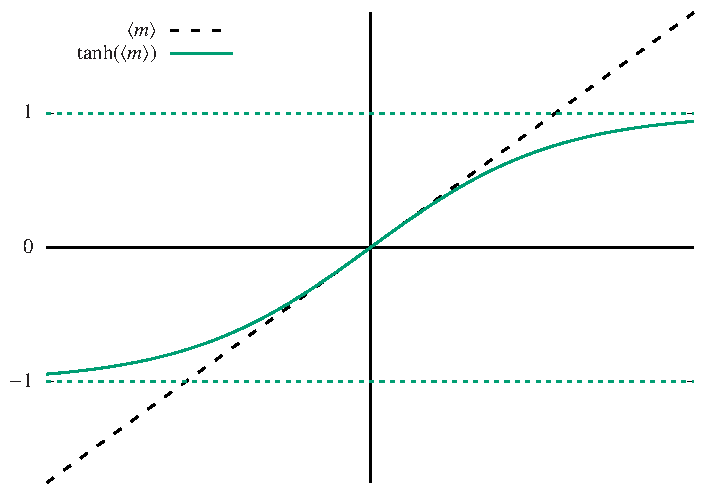
\includegraphics[width=0.69\textwidth]{figs/unit09_consistency.pdf}\end{center}

To confirm our interpretation of this result, let's check how the intersections depend on \be and $H$.
In the next plot below we keep the same temperature $T = 1 / \be = 4$ while comparing two non-zero values for the external magnetic field.
A positive $H = 2$ simply shifts $g(\vev{m})$ to the left (the green line), while a negative $H = -2$ shifts it to the right (the blue line).
In both cases there is still only a single intersection, at $\vev{m} \approx \pm 0.88$ for $H = \pm 2$.
We can interpret this non-zero result as an indication that the system is in an ordered phase where the spins tend to align with the external field. \\[-24 pt]
\begin{center}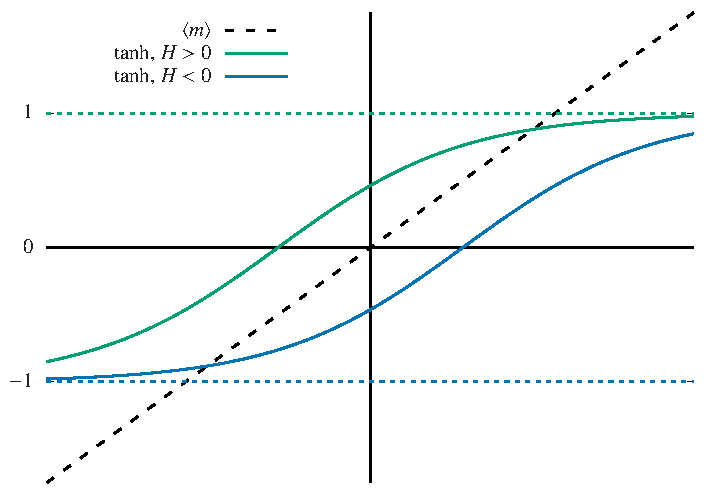
\includegraphics[width=0.69\textwidth]{figs/unit09_consistency_H.pdf}\end{center}

From our work in the previous section, we can expect that the spins' alignment will increase --- reflecting the minimum-energy ground states --- as the temperature decreases.
Decreasing the temperature increases $\be$, which causes the argument of the $\tanh$ to vary more rapidly with $\vev{m}$, making $g(\vev{m})$ a steeper function that more rapidly approaches its limiting values $\pm 1$.
The plot below illustrates this for $T = 1 / \be = 2$.
For this temperature with magnetic field $H = \pm 2$, the intersection is $\vev{m} \approx \pm 1$ to a very good approximation.
We can also appreciate that $-1 \leq \tanh x \leq 1$ ensures that the mean-field self-consistency condition can only ever be satisfied for $-1 \leq \vev{m} \leq 1$, reassuringly consistent with the definition of the magnetization. \\[-24 pt]
\begin{center}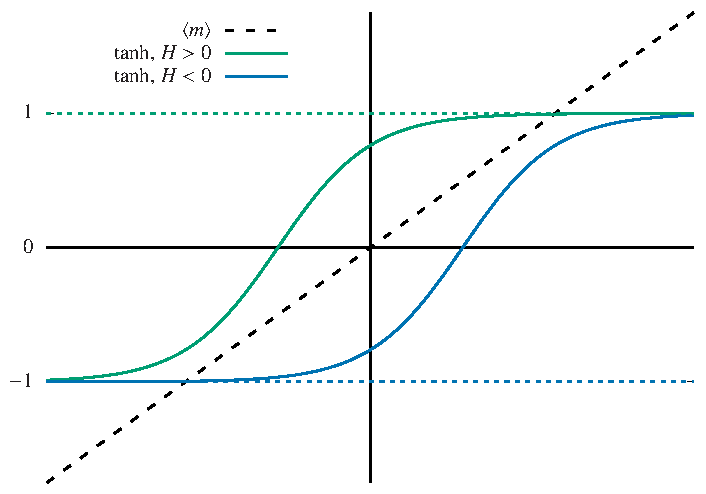
\includegraphics[width=0.69\textwidth]{figs/unit09_consistency_H-beta.pdf}\end{center}

Also in the previous section, we saw that the Ising model spins should align at low temperatures, even without an external field to promote one direction over the other.
To check whether this behaviour is preserved by the mean-field approximation, we can consider the self-consistency condition for various temperatures with $H = 0$.
The plot below shows the results, considering a low temperature $T = 2$ (the blue line), the same $T = 4$ green curve shown in the first plot above, and a high temperature $T = 8$ (the red line).
While the $\vev{m} = 0$ expected in the disordered phase is always a possible solution, something interesting happens at lower temperatures, where the steeper $\tanh$ function introduces two additional solutions at non-zero $\vev{m} = \pm m_0$ corresponding to the ordered phase.
As $T \to 0$, this magnetization approaches its maximum value $m_0 \to 1$. \\[-24 pt]
\begin{center}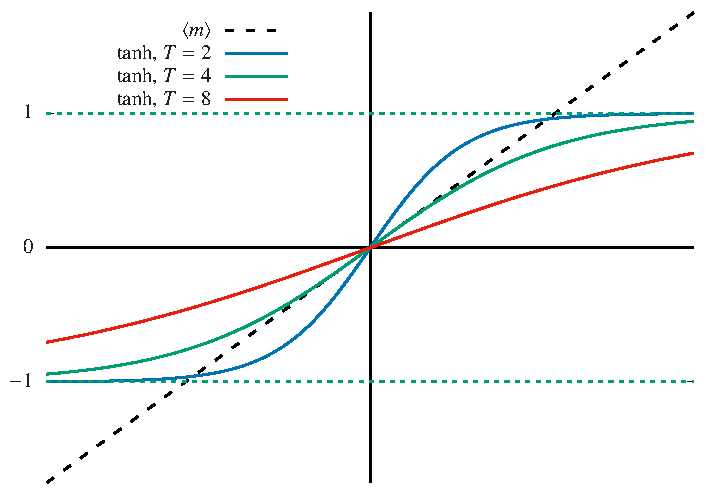
\includegraphics[width=0.69\textwidth]{figs/unit09_consistency_beta.pdf}\end{center}

When there are three solutions $\vev{m} = \left\{-m_0, 0, m_0\right\}$ at low temperatures, we can determine that the $\vev{m} = 0$ solution is actually \textit{unstable}.
Here we are venturing briefly into non-equilibrium territory, and thinking of the mean-field system as a `blind' process that attempts to satisfy the self-consistency condition $\vev{m} = \tanh\left[2\be d\vev{m}\right]$, based only on whether the expectation value of the magnetization is too small or too large compared to the $\tanh$.
Once the magnetization is self-consistent, the system can happily settle into thermodynamic equilibrium.

From the figure above we can see that with $H = 0$ we can have three solutions only when the slope of the $\tanh$ at $\vev{m} = 0$ is greater than $1$.
Any positive value $\vev{m} = \varepsilon > 0$ would then produce $\tanh\left[2\be d\vev{m}\right] > \vev{m}$, which the system `feels' as a magnetization that is too small to be self-consistent.
This drives the system to continue increasing its magnetization, until it eventually settles at the non-zero solution $\vev{m} = m_0$.
Similarly, any negative magnetization $\vev{m} = -\varepsilon < 0$ would drive $\vev{m}$ away from zero and to the $\vev{m} = -m_0$ solution.

This argument can be visualized more easily by plotting $\tanh\left[2\be d\vev{m}\right] - \vev{m}$ vs.\ $\vev{m}$ as shown in the final plot below.
When this difference is negative, $\vev{m}$ is larger than the self-consistency condition allows, driving the system to smaller $\vev{m}$ as shown by the arrows pointing to the left.
Conversely, when the difference is positive, the system `seeks' self-consistency by increasing $\vev{m}$ as shown by the arrows pointing to the right.
For the low temperature $T = 2$, we see that the arrows move the system away from the unstable solution $\vev{m} = 0$ and to the stable solutions $\vev{m} = \pm m_0$.

\begin{center}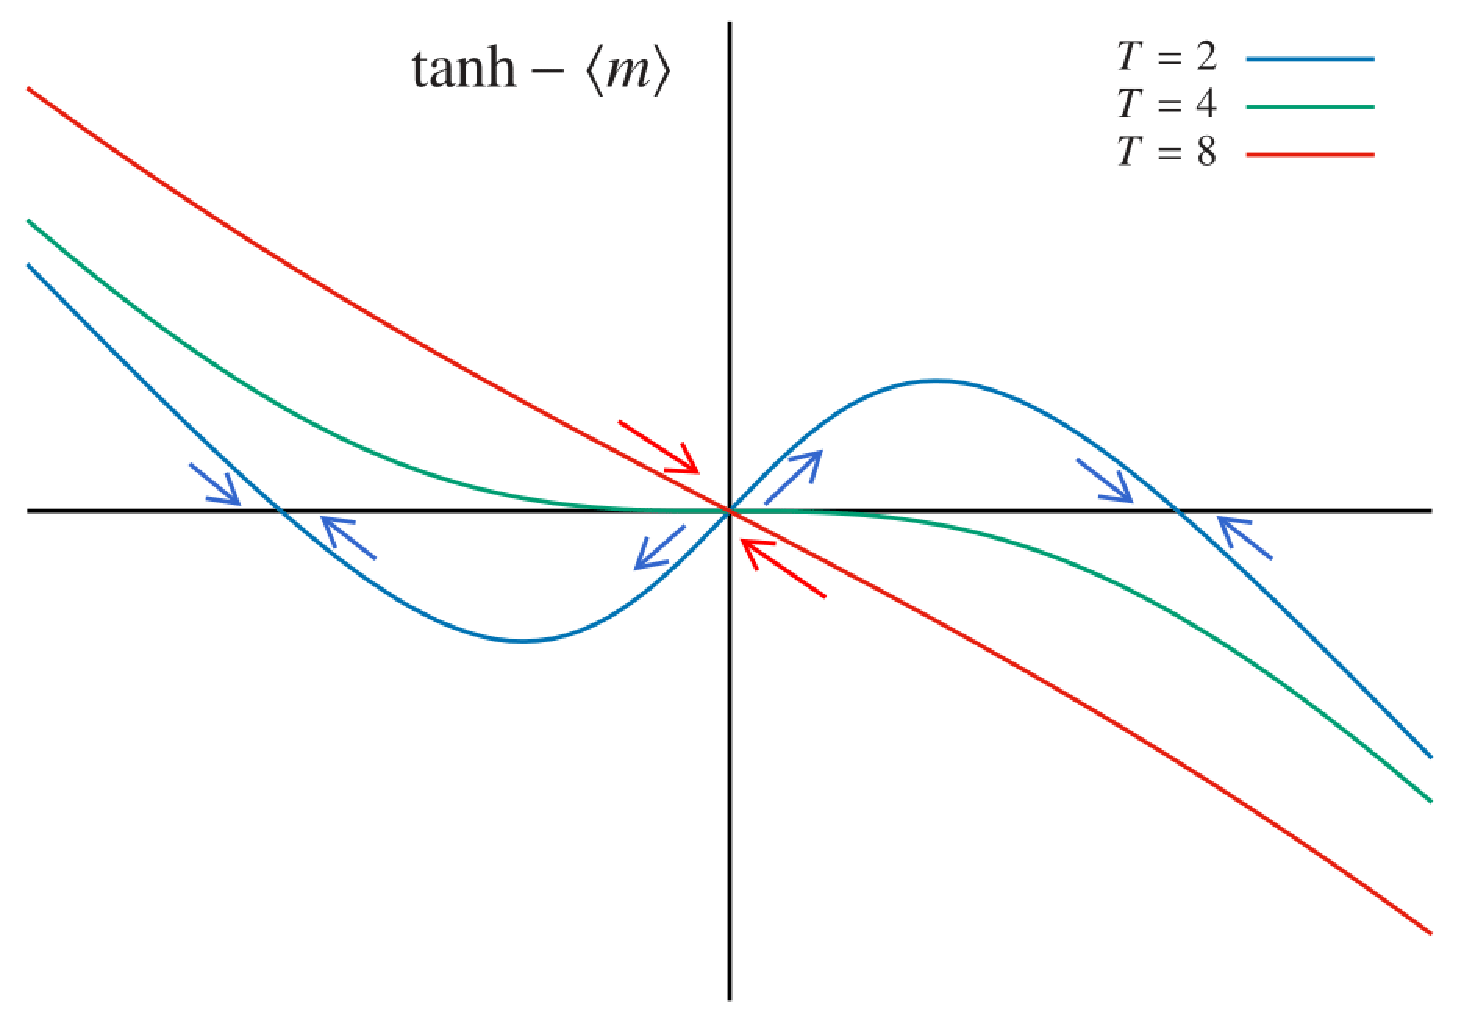
\includegraphics[width=0.7\textwidth]{figs/unit09_consistency_flow.pdf}\end{center}

At this point we can conclude that the non-interacting mean-field approximation successfully captures at least the high- and low-temperature limits of the interacting zero-field Ising model that we determined in the previous section.
For high temperatures the mean-field self-consistency condition demands $\vev{m} = 0$ in the disordered phase, while for low temperatures it produces $\vev{m} = \pm m_0 \ne 0$ in the ordered phase.

Going further, now that we have a more tractable non-interacting system we can determine the value of the temperature at which its $\vev{m} = \pm m_0$ solutions appear and the $\vev{m} = 0$ solution becomes unstable.
As described above, this occurs whenever the slope of the $\tanh$ function at $\vev{m} = 0$ is greater than $1$.
Let's call the corresponding temperature $T_c$, though it remains to be determined whether it is really the critical temperature of a true phase transition.
Expanding $\tanh(x)$ for $x \approx 0$, what is $T_c$?
\begin{mdframed}
  \ \\[50 pt]
\end{mdframed}

You should find that the change from the high-temperature disordered phase to the low-temperature ordered phase occurs at $T_c = 2d$ in $d$ dimensions, or equivalently $\be_c = \frac{1}{2d}$ --- corresponding to the green lines in the two figures above with $d = 2$.
In order to determine whether or not this is a true critical temperature, we need to check whether the order parameter $\vev{m}$ or its $T$-derivatives are discontinuous at $T_c$.
We can do this by considering the self-consistency condition for a temperature $T$ lower than but very near to $T_c = 2d$, which would produce $0 < |\vev{m}| \ll 1$ and allow us to expand $\tanh(x) = x - \frac{x^3}{3} + \cO\left(x^5\right)$.
What is the resulting prediction for $\vev{m}$?
\begin{mdframed}
  \ \\[100 pt]
\end{mdframed}

Making the approximation $\left(\frac{T}{T_c}\right)^2 \approx 1$, your result should resemble
\begin{equation*}
  \vev{m} = \pm \sqrt{3} \left(\frac{T_c - T}{T_c}\right)^{1 / 2} \qquad \mbox{for } \ T \lesssim T_c.
\end{equation*}
From this, we can see that the order parameter $\vev{m}$ is continuous at $T_c$:
\begin{equation}
  \vev{m} \propto \left\{\begin{array}{cl} \left(T_c - T\right)^{1 / 2} & \mbox{for } \ T \lesssim T_c \\[3 pt]
                                           0                            & \mbox{for } \ T \gtrsim T_c\end{array}\right. .
\end{equation}
However, its first derivative
\begin{equation*}
  \frac{d\vev{m}}{dT} \propto \frac{1}{\left(T_c - T\right)^{1 / 2}}
\end{equation*}
diverges as $T \to T_c$ from below.
This is the situation we discussed at the end of the previous section, which predicts a second-order phase transition with critical temperature $T_c = 2d$ in $d$ dimensions.
The power-law dependence $\vev{m} \propto \left(T_c - T\right)^b$ with $0 < b < 1$ is a generic feature of second-order phase transitions.
The power $b$ is known as a \textbf{critical exponent}, in this case $b = 1 / 2$.

At this point we have invested some effort to find that the mean-field approximation of the $d$-dimensional Ising model, with $H = 0$, predicts a second-order phase transition at $T_c = 2d$ with critical exponent $1 / 2$.
Let's wrap up this section with some quick comments on the reliability of the mean-field approximation and the accuracy of these results it has given us.

The accuracy of the mean-field results turns out to depend on the number of dimensions.
For the one-dimensional Ising model that Ising himself solved, there is no phase transition at all, as we will derive in the next section.
In other words, the mean-field approximation simply fails for $d = 1$.

The situation improves for the two-dimensional Ising model.
Onsager's exact $H = 0$ solution features a second-order phase transition, at an inverse critical temperature $\be_c = \frac{1}{2} \log\left(1 + \sqrt{2}\right) \approx 0.44$ that had been exactly determined a few years before his work.
For $T \lesssim T_c$, the magnetization vanishes as $\vev{m} \propto \left(T_c - T\right)^{1 / 8}$, corresponding to a critical exponent $1 / 8$.
While the mean-field prediction of a second-order phase transition is now qualitatively correct, at a quantitative level its predicted $\be_c = \frac{1}{2d} = 0.25$ is off by almost a factor of $2$, while the mean-field critical exponent $b = 1 / 2$ is four times larger than the true $b = 1 / 8$.

For higher dimensions $d \geq 3$ there is no known exact solution for the Ising model, but the existence of a second-order phase transition can be established and the corresponding critical temperature and critical exponents can be computed numerically, as we will discuss in Unit~10.
In three dimensions the mean-field $T_c = 2d = 6$ and $b = 1 / 2$ are still significantly different from the true $T_c \approx 4.5$ and $b \approx 0.32$. % From Tong and arXiv:1806.03558
The mean-field prediction for the critical exponent $b = 1 / 2$ turns out to be correct for $d \geq 4$, while the critical temperature $T_c = 2d$ gradually approaches the true value as the number of dimensions increases.
Numerical computations find $T_c \approx 6.7$, $8.8$, $10.8$, $12.9$ and $14.9$ for $d = 4$, $5$, $6$, $7$ and $8$, respectively, so that the mean-field result improves from being $\sim$$19\%$ too high for $d = 4$ to only $\sim$$7\%$ too high for $d = 8$. % From arXiv:1202.3031, arXiv:1502.07613 and arXiv:0807.2546
Formally, the mean-field approximation exactly reproduces the Ising model in the abstract limit of infinite dimensions, $d \to \infty$.
Roughly speaking, the greater reliability of the mean-field approach in higher dimensions is due to the larger number of nearest neighbours for each site, $2d$.
The larger number of nearest-neighbour spins produces a more reliable approximation of the mean spin in the effective field seen by each site in the mean-field approach.
% ------------------------------------------------------------------



% ------------------------------------------------------------------
\subsection{Exact results for the Ising model}
If time permits, it is not too hard to prove some of the exact results mentioned above, for the Ising model in one and two dimensions where the mean-field approximation is least reliable.

\subsubsection{One-dimensional partition function and magnetization}
The special property of the one-dimensional Ising model that helps us derive a closed-form expression for its partition function is the fact that it has exactly as many links as it has sites.
Looking back to the illustration on page~130, we can rewrite the nearest-neighbour interaction term as
\begin{equation*}
  \sum_{(jk)} s_j s_k = \sum_{n = 1}^N s_n s_{n + 1},
\end{equation*}
where the periodic boundary conditions identify $s_{N + 1} = s_1$.
If we also rewrite the magnetic-field term as $H \sum_{n = 1}^N s_n = \frac{H}{2} \sum_{n = 1}^N \left(s_n + s_{n + 1}\right)$, then the full internal energy is
\begin{equation*}
  E_i = -\sum_{n = 1}^N \left[s_n s_{n + 1} + \frac{H}{2}\left(s_n + s_{n + 1}\right)\right].
\end{equation*}
Inserting this into the partition function $Z(\be, N, H) = \sum_{\left\{s_n\right\}} \exp\left[-\be E(s_n)\right]$, we can convert the exponential of the sum into a product of exponentials,
\begin{equation*}
  Z = \sum_{s_1 = \pm 1} \cdots \sum_{s_N = \pm 1} \prod_{n = 1}^N \exp\left[\be s_n s_{n + 1} + \frac{\be H}{2}\left(s_n + s_{n + 1}\right)\right].
\end{equation*}

Similarly to \eq{eq:spin_part_func} for the non-interacting case, we are going to distribute the summations.
Now, however, we have to keep track of the fact that a given spin $s_j$ will appear both when $n = j$ and when $n + 1 = j$, and for each spin configuration it must have the same value both times it appears.
An elegant way to account for all allowed possibilities is through matrix multiplication.
Use the $2\times 2$ matrix
\begin{equation}
  T_n = \begin{pmatrix} e^{\be + \be H} & e^{-\be} \\ e^{-\be} & e^{\be - \be H} \end{pmatrix}
\end{equation}
to collect the exponential factors for the four possibilities
\begin{equation*}
  \left\{s_n, s_{n + 1}\right\} = \begin{pmatrix} \left\{1, 1\right\} & \left\{1, -1\right\} \\ \left\{-1, 1\right\} & \left\{-1, -1\right\} \end{pmatrix}.
\end{equation*}
The matrix product $T_n \cdot T_{n + 1}$ then provides the sum over all contributions with consistent values for $s_{n + 1}$.
Repeating this for all terms in $\prod_{n = 1}^N$, the periodic boundary conditions produce the (cyclic) trace, making the exact partition function simply
\begin{equation*}
  Z = \mbox{Tr}\left[\prod_{n = 1}^N T_n \right].
\end{equation*}
What's more, since $T_n \equiv T$ is actually independent of $n$, this simplifies further to
\begin{equation}
  Z = \mbox{Tr}\left[T^N \right].
\end{equation}

$T$ is known as the \textbf{transfer matrix} --- roughly speaking, it `transfers' information about the values of the spins from one link to the next.
At this point we can appreciate that our earlier rewriting of the magnetic-field term in the energy just helped to make $T$ more symmetric.
If we now diagonalize
\begin{equation*}
  T = \begin{pmatrix} e^{\be} e^{\be H} & e^{-\be} \\ e^{-\be} & e^{\be} e^{-\be H} \end{pmatrix} \quad \lra \quad \begin{pmatrix} \la_+ & 0 \\ 0 & \la_- \end{pmatrix},
\end{equation*}
the partition function will become simply
\begin{equation*}
  Z = \mbox{Tr}\left[\begin{pmatrix} \la_+ & 0 \\ 0 & \la_- \end{pmatrix}^N\right] = \mbox{Tr}\begin{pmatrix} \la_+^N & 0 \\ 0 & \la_-^N \end{pmatrix} = \la_+^N + \la_-^N.
\end{equation*}
\newpage
\noindent What are the two eigenvalues $\la_{\pm}$ of $T$?
\begin{mdframed}
  \ \\[120 pt]
\end{mdframed}

With $\be \geq 0$ and $H \geq 0$, we can check that both eigenvalues are real and $\la_+ > \la_-$.
For asymptotically high temperatures, $\be \to 0$, the eigenvalues reduce to $\la_+ = 2$ and $\la_- = 0$ independent of $H$.
In the special case $H = 0$, the eigenvalues are $\la_+ = 2\cosh\be$ and $\la_- = 2\sinh\be$, while $H > 0$ typically produces $\la_+ \gg \la_-$.
Because $\la_- / \la_+ < 1$, for sufficiently large $N \gg 1$ we can further simplify
\begin{equation*}
  Z = \la_+^N\left[1 + \left(\frac{\la_-}{\la_+}\right)^N \right] \approx \la_+^N = e^{N\be} \cosh^N(\be H)\left[1 + \sqrt{1 - \frac{2\sinh(2\be)}{e^{2\be}\cosh^2(\be H)}}\right]^N.
\end{equation*}

So there we have it --- the solution of the Ising model in one dimension.
As usual, the partition function $Z$ is not so revelatory in and of itself.
Its principal value lies in enabling us to predict observables like the magnetization --- so let's do that, returning to the zero-field case for which we computed the mean-field critical temperature and critical exponent in the previous section:
\begin{mdframed}
  \ \\[80 pt]
\end{mdframed}
Note that we set $H = 0$ only \textit{after} computing the derivative of the free energy, which allows us to consider $\vev{m}$ rather than $\vev{|m|}$.
Upon setting $H = 0$, something remarkable happens: $\vev{m} = 0$ for all temperatures!

As claimed at the end of the previous section, the zero-field one-dimensional Ising model has no phase transition at all.
It is always in the disordered phase, even in the limit of absolute zero $T \to 0$.
In addition to showing that the mean-field approximation fails in one dimension, this result also reveals how the balance of energy level degeneracy vs.\ Boltzmann factor considered in \secref{sec:Ising_phases} depends on the lattice structure.

Specifically, for the case of a one-dimensional lattice, the first excited energy level with energy $E_1$ includes more micro-states than the $2N$ we get by flipping a single spin to oppose the full alignment of the ground state.
Suppose we start from the ground state and flip spin $s_j$ to reach the first excited energy level.
Relative to the ground-state energy $E_0 = -N$, the energy of this micro-state is increased to $E_1 = -N + 4$ due to the positive contributions from the $s_{j - 1} s_j$ and $s_j s_{j + 1}$ links.
But if we now consider \textit{also} flipping spin $s_{j + 1}$, the $s_j s_{j + 1}$ link goes back to providing a negative contribution while the positive contribution shifts to the $s_{j + 1} s_{j + 2}$ link.
This gives us an additional $2N$ micro-states featuring a flipped nearest-neighbour \textit{pair} of spins, with the same energy $E_1$ but a smaller magnetization $|m| = 1 - \frac{4}{N}$.
And we can continue this process, finding more degenerate micro-states with a flipped block of \textit{any} number of neighbouring spins up to $N - 1$, and hence any magnetization, including $m = 0$.

The non-existence of an ordered phase in one dimension also holds for more general interacting systems beyond just the Ising model.
A useful way to analyse this sort of behaviour is to describe all of the micro-states in the first excited energy level as consisting of two \textit{domains} separated by two \textbf{domain walls} (recalling the periodic boundary conditions).
For the Ising model, one domain will contain only up spins while the other will contain only down spins.
The two domain walls are able to move freely through the lattice without changing the energy, but as the domain walls move the magnetization samples the full range of values $-\left(1 - \frac{2}{N}\right) \leq m \leq 1 - \frac{2}{N}$.

\subsubsection{Two-dimensional critical temperature}
While the zero-field Ising model on the $d = 2$ square lattice has also been exactly solved, both Onsager's original calculation and subsequent re-derivations using simpler techniques are much too complicated to cover here.
However, a few years before Onsager published his famous result, \href{https://en.wikipedia.org/wiki/Hans_Kramers}{Hans Kramers} and \href{https://en.wikipedia.org/wiki/Gregory_Wannier}{Gregory Wannier} were able to determine the exact $d = 2$ critical temperature \href{https://doi.org/10.1103/PhysRev.60.252}{in 1941}.
They did this by identifying a relation between two Ising model partition functions, without actually evaluating either sum over micro-states:
\begin{equation}
  \label{eq:dual_Z}
  \frac{Z(\be)}{2^N \cosh^{2N} \be} = \frac{Z(\betw)}{2e^{2N\betw}},
\end{equation}
where the two inverse temperatures \be and \betw are related by
\begin{equation}
  \label{eq:dual_beta}
  \sinh(2\be) = \frac{1}{\sinh(2\betw)}.
\end{equation}
This relation is now known as \href{https://en.wikipedia.org/wiki/Kramers-Wannier_duality}{Kramers--Wannier duality}, and the general concept of \textbf{duality} has become a powerful tool in modern theoretical physics.
Note that small \be implies large \betw and vice versa --- the duality relates one $d = 2$ Ising model at a high temperature to another one at a low temperature.

Although it can be useful to explicitly compare such high- and low-temperature partition functions, by computing series expansions as we did for the non-interacting spin system in \secref{sec:spin_info} and for the Einstein solid in tutorial exercises, we'll skip that exercise, to keep this section from becoming too long.
Those who are interested can find related discussions in Sections~5.3.2 and 5.3.3 of David Tong's \href{https://www.damtp.cam.ac.uk/user/tong/statphys.html}{\textit{Lectures on Statistical Physics}}.
Some of the manipulations below, which may seem to come out of thin air, can be motivated by considering these expansions.

The first manipulation is to express the zero-field partition function as
\begin{equation*}
  Z = \sum_{\left\{s_n\right\}} \exp\left[\be\sum_{(jk)} s_j s_k\right] = \sum_{\left\{s_n\right\}} \prod_{(jk)} \exp\left[\be s_j s_k\right] = \sum_{\left\{s_n\right\}} \prod_{(jk)} \left[\cosh \be + s_j s_k \sinh \be\right],
\end{equation*}
which relies on the fact $s_j s_k = \pm 1$ for the Ising model.
It's easy to check the relation $e^{\be s_j s_k} = \cosh \be + s_j s_k \sinh \be$ for both $s_j s_k = 1$ and $s_j s_k = -1$:
\begin{mdframed}
  \ \\[80 pt]
\end{mdframed}
Next, we write the sum over the $\cosh$ and $\sinh$ as a summation,
\begin{equation*}
  Z = \sum_{\left\{s_n\right\}} \prod_{(jk)} \left[\cosh \be + s_j s_k \sinh \be\right] = \sum_{\left\{s_n\right\}} \prod_{(jk)} \sum_{p_{jk} = 0, 1} C_{p_{jk}}(\be) (s_j s_k)^{p_{jk}},
\end{equation*}
by defining $C_0(\be) \equiv \cosh \be$ and $C_1(\be) \equiv \sinh \be$ while raising $s_j s_k$ to the corresponding power $p_{jk}$.
Recall that the nearest-neighbour pairs $(jk)$ correspond to all $2N$ links in the $d = 2$ lattice.
To make the language a little less awkward, we can say that $p_{jk} = 1$ corresponds to link $jk$ being `on' while $p_{jk} = 0$ when it is turned `off'.
The product and sum above account for all possible configurations of links that are turned on and off, which we can more conveniently represent as another configuration sum,
\begin{equation*}
  \sum_{\left\{p\right\}} \equiv \sum_{p_1 = 0, 1} \cdots \sum_{p_{2N} = 0, 1}.
\end{equation*}

Our partition function is now written in terms of two configuration sums, but we can expect only one to be necessary.
We will aim to eliminate the sum over all spin configurations, by pulling out everything independent of the spins:
\begin{equation*}
  Z = \sum_{\left\{s_n\right\}} \sum_{\left\{p\right\}} \prod_{(jk)} C_{p_{jk}}(\be) (s_j s_k)^{p_{jk}} = \sum_{\left\{p\right\}} \left[\prod_{(jk)} C_{p_{jk}}(\be)\right] \sum_{\left\{s_n\right\}} \left[\prod_{(jk)} s_j^{p_{jk}} s_k^{p_{jk}}\right].
\end{equation*}
The final factor can be converted from a product over links to a product over sites.
For $d = 2$, any spin $s_n$ will appear four times in the product, once for each of the four links connected to it.
The product of these four factors can be rewritten as
\begin{align*}
  \prod_{(nk)} s_n^{p_{nk}} & = s_n^{P_n}, &
  \mbox{defining } \ P_n & \equiv \sum_{(nk)} p_{nk}.
\end{align*}

We are now left with a product over individual $s_n$:
\begin{equation*}
  Z = \sum_{\left\{p\right\}} \left[\prod_{(jk)} C_{p_{jk}}(\be)\right] \sum_{\left\{s_n\right\}} \left[\prod_{n = 1}^N s_n^{P_n}\right].
\end{equation*}
Although each $s_n$ is raised to a power that depends on $p_{nk}$ for all four of its links to its nearest neighbours, consider what happens when we sum over the two values $s_n = \pm 1$.
There are two possibilities: If $P_n$ is odd, then the $s_n = 1$ and $s_n = -1$ contributions cancel --- making the entire product over sites vanish!
Otherwise, if $P_n$ is even, they add up to give twice the product over the other sites.
Repeating for all sites, the only non-zero contribution must have $N$ factors of $2$:
\begin{equation}
  \label{eq:constrained_Ising}
  Z = \sum_{\left\{p\right\}} \prod_{(jk)} C_{p_{jk}}(\be) \prod_{n = 1}^N 2\de_2(P_n) = 2^N \sum_{\left\{p\right\}} \prod_{(jk)} C_{p_{jk}}(\be) \prod_{n = 1}^N \de_2\left(\Sigma_{(nk)} p_{nk}\right),
\end{equation}
where the `mod-$2$' Kronecker delta $\de_2(P_n)$ vanishes if $P_n$ is odd and equals one if $P_n$ is even.

We have successfully eliminated the spin configuration sum $\left\{s_n\right\}$ in \eq{eq:constrained_Ising}, which no longer explicitly refers to our original degrees of freedom at all!
In its place we now have a configuration sum over all on-or-off links --- $p_{jk} = 1$ or $0$, respectively.
And there is a very tricky set of $N$ inter-dependent constraints coming from the product of $\de_2$ factors, which require that an even number of links be turned on at \textit{every} lattice site, in order to get a non-zero contribution to the partition function.
This is a sign that our new variables $p_{jk}$ aren't entirely independent of each other --- which makes sense, since we have $2N$ of them, but started off with only $N$ degrees of freedom.

What we can do about these constraints?
Well, the constraints arose as a result of eliminating a configuration sum over $s_n = \pm 1$, so it is at least plausible that we can unwind them by introducing a \textit{different} set of spin variables, $\stw_n = \pm 1$.
We want the $\pm 1$ values of $\stw_n$ to be related to the $\left\{0, 1\right\}$ values of $p_{jk}$, which we can achieve by implicitly defining $\stw_n$ via
\begin{align*}
  p_{12} & = \frac{1 - \stw_1 \stw_2}{2} &
  p_{13} & = \frac{1 - \stw_2 \stw_3}{2} \\
  p_{14} & = \frac{1 - \stw_3 \stw_4}{2} &
  p_{15} & = \frac{1 - \stw_1 \stw_4}{2}
\end{align*}
and so on for all $2N$ links.
A convenient way to keep track of the subscripts above is to identify these $\stw_n$ with the \textbf{dual lattice} drawn on the next page.
Each $\stw_n$ is identified with one of the $N$ plaquettes of the original lattice, and pairs $\stw_a$ and $\stw_b$ determine $p_{jk}$ for the link passing between them. \\[-24 pt]
\begin{center}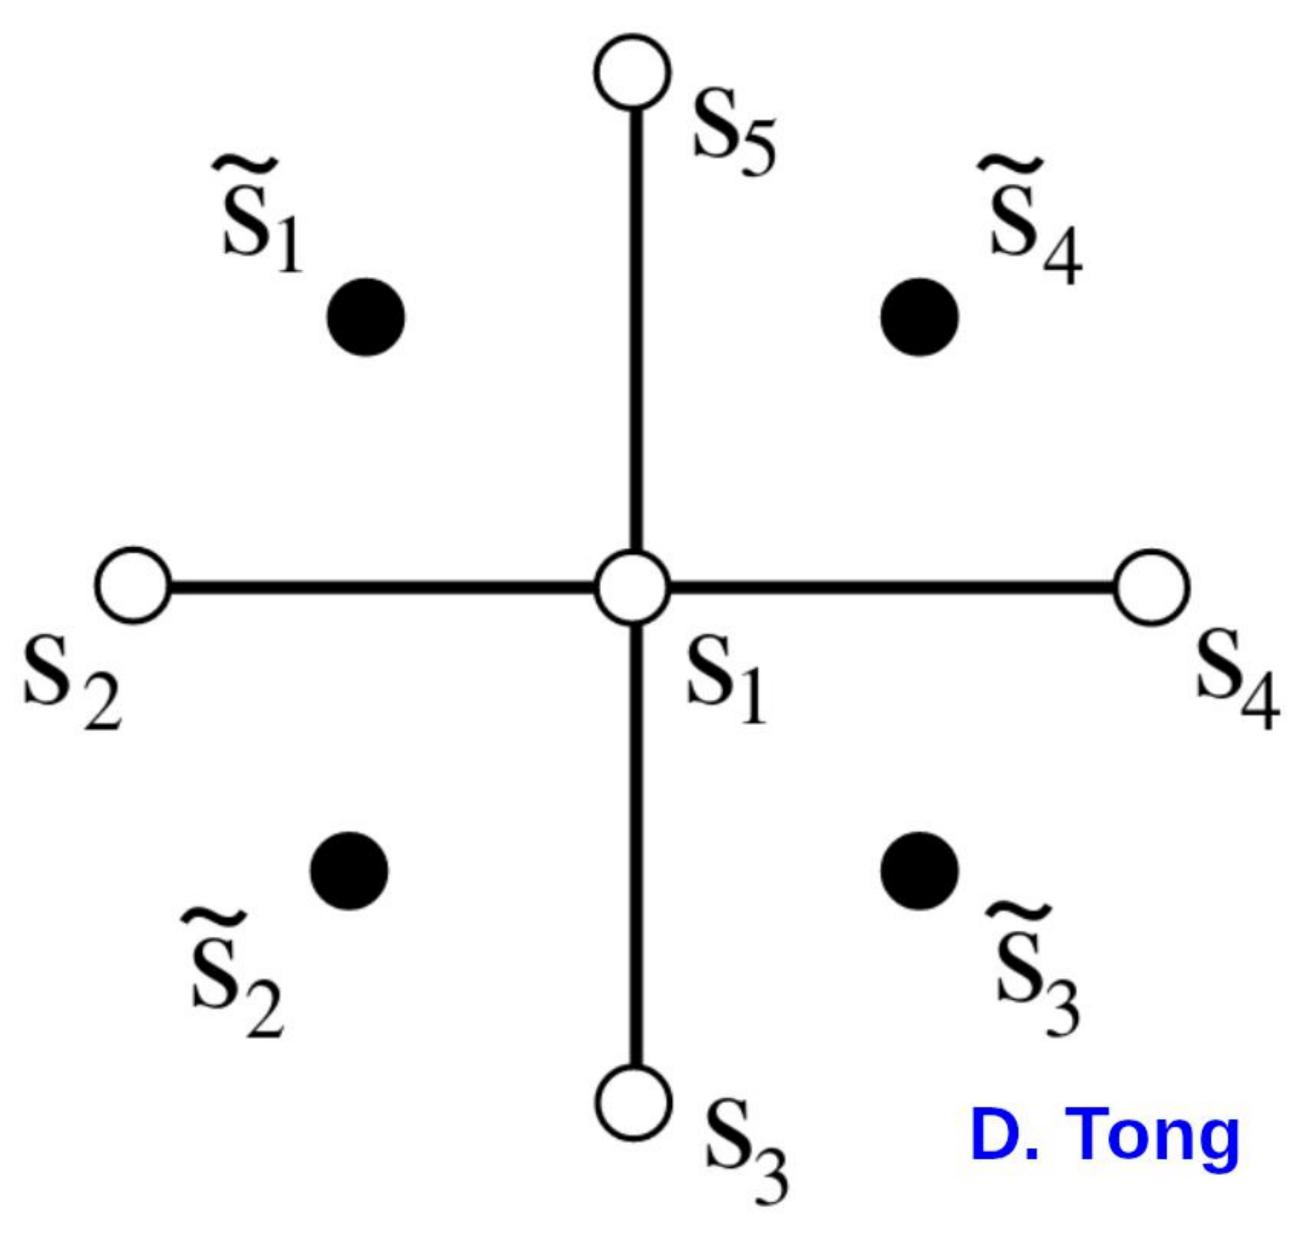
\includegraphics[width=0.46\textwidth]{figs/unit09_dual_lattice.pdf}\end{center}

This provides another way to see that $p_{jk}$ aren't completely independent variables: Both $p_{12}$ and $p_{15}$ depend on $\stw_1$, both $p_{12}$ and $p_{13}$ depend on $\stw_2$, and so on.
Delightfully, these patterns of dependence are precisely what we need to handle the $\de_2$ factors that are still in our partition function.
If we consider
\begin{align*}
  P_1 & = p_{12} + p_{13} + p_{14} + p_{15} = 2 - \frac{\stw_1 \stw_2 + \stw_2 \stw_3 + \stw_3 \stw_4 + \stw_1 \stw_4}{2} \\
      & = 2 - \frac{(\stw_1 + \stw_3)(\stw_2 + \stw_4)}{2} \in \left\{0, 2, 4\right\},
\end{align*}
we see that working in terms of $\stw_n$ automatically turns on an even number of links at every site, producing $\prod_{n = 1}^N \de_2(P_n) = 1$!

In order to replace $\sum_{\left\{p\right\}}$ by $\sum_{\left\{\stw\right\}}$, we need to confirm that the latter accounts for all possible $P_n = \left\{0, 2, 4\right\}$.
It turns out that the dual-spin configuration sum provides all values of $P_n$ twice, which we can check for the simple case $P_1 = 4$: % TODO: 1+6+1 ways of getting P_1 = 0, 2, 4 account for all 2+12+2=16 = 2^4 combinations of spins...
\begin{mdframed}
  \ \\[50 pt]
\end{mdframed}
This generalizes to the full $N$-spin system: Negating all $\stw_n \to -\stw_n$ leaves all $P_n$ unchanged.\footnote{This is discussed in more detail by Robert Savit, ``\href{https://doi.org/10.1103/RevModPhys.52.453}{Duality in field theory and statistical systems}'', \textit{Reviews of Modern Physics} \textbf{52} (1980), 453.}
Therefore converting the partition function from \eq{eq:constrained_Ising} into a configuration sum over $\left\{\stw\right\}$ gives us
\begin{equation*}
  Z = \frac{1}{2} 2^N \sum_{\left\{\stw\right\}} \prod_{(jk)} C_{(1 - \stw_j \stw_k) / 2}(\be),
\end{equation*}
where $(jk)$ now refers to the dual lattice.

The final step is to express $C_0(\be) = \cosh \be$ and $C_1(\be) = \sinh \be$ in terms of the dual variables $\stw_n$ that we're now working with.
The trick here is to write
\begin{equation*}
  C_p(\be) = \left(\cosh \be\right) \exp\left[p \log \tanh \be\right] = \left(\cosh \be\right) \exp\left[\frac{1 - \stw_j \stw_k}{2} \log \tanh \be\right],
\end{equation*}
substituting $p = (1 - \stw_j \stw_k) / 2$.
Breaking up the exponential gives us
\begin{equation*}
  C_p(\be) = \left(\cosh\be \sinh\be\right)^{1 / 2} \exp\left[-\frac{1}{2} \stw_j \stw_k \log \tanh \be\right].
\end{equation*}
Inserting this into the partition function, the product over all links just provides $2N$ factors of the $\stw_n$-independent first term, and we can then convert the product of exponentials into an exponential of the sum, producing
\begin{equation*}
  Z = \frac{1}{2} \left(2\cosh\be \sinh\be\right)^N \sum_{\left\{\stw\right\}} \exp\left[-\frac{\log \tanh \be}{2} \sum_{(jk)} \stw_j \stw_k\right].
\end{equation*}

By defining $\betw \equiv -\frac{1}{2}\log \tanh \be$, we can recognize the sum over $\left\{\stw\right\}$ configurations as simply a zero-field Ising model partition function $Z(\betw)$, \eq{eq:Ising_zero_field}.
We can also confirm that this definition of \betw is equivalent to \eq{eq:dual_beta}:
\begin{mdframed}
  \ \\[100 pt]
\end{mdframed}
Using similar manipulations, we can express the spin-independent prefactor in terms of either \be or $\betw$,
\begin{equation*}
  2\cosh\be \sinh\be = \sinh(2\be) = \frac{1}{\sinh(2\betw)},
\end{equation*}
or in the mixed form that reproduces \eq{eq:dual_Z}:
\begin{equation*}
  2\cosh\be \sinh\be = 2\cosh^2 \be \tanh\be = \frac{2\cosh^2 \be}{e^{2\betw}} \quad \implies \quad \frac{Z(\be)}{\left(2\cosh^2\be\right)^N} = \frac{Z(\betw)}{2e^{2N\betw}}.
\end{equation*}

We have successfully derived Kramers--Wannier duality!
Now let's briefly interpret what it means.
It's a worthwhile \textbf{exercise} to show that multiplying a partition function by an overall spin-independent factor, $Z(\be) \to c(\be) Z(\be)$, has no effect on expectation values.
(Try it!)
Therefore the relation above identifies a $d = 2$ Ising system at temperature $1 / \be$ with another such system at temperature $1 / \betw$, where small \be corresponds to large \betw and vice versa.

This does \textit{not} mean that $d = 2$ Ising model behaves the same at low and high temperatures.
Indeed, we saw already in \secref{sec:Ising_phases} that it changes between qualitatively different ordered and disordered phases in these two regimes.
What Kramers--Wannier duality is telling us is that the ordered phase of Ising spins in two dimensions, characterized by their order parameter, is secretly equivalent to the disordered phase of the \textit{dual} spins --- a different set of degrees of freedom, which can be characterized by a `disorder parameter'.
Similarly, the disordered phase of the original system maps onto the ordered phase of the dual system.

If we assume there is a single phase transition where the ordered and disordered phases coincide (which \href{https://en.wikipedia.org/wiki/Rudolf_Peierls}{Rudolf Peierls} had established in 1936), then Kramers--Wannier duality implies this must occur when $\be = \betw$.
In other words,
\begin{equation*}
  \sinh^2(2\be_c) = 1 \quad \Lra \quad \be_c = \frac{1}{2} \mathrm{arcsinh}(1) = \frac{\log\left(1 + \sqrt{2}\right)}{2} = 0.440686\dots,
\end{equation*}
recalling (or looking up) that $\mathrm{arcsinh}(x) = \log\left(x + \sqrt{x^2 + 1}\right)$.
Because this exact critical temperature $T_c = 2 / \log\left(1 + \sqrt{2}\right) = 2.269185\dots$ was predicted three years before Onsager analytically solved the $d = 2$ Ising model, the fact that his solution reproduced it was an important check of correctness.

As mentioned at the start of this subsection, dualities of this sort are central to theoretical physics in the 21st century.
In general, these dualities are much more complicated than Kramers--Wannier duality, in two main ways.
First, the dual degrees of freedom are typically different --- and have different interactions --- than the original degrees of freedom.
For example, if we were to carry out a similar analysis of the three-dimensional Ising model, we would find that the dual system is \textit{not} just another Ising model. % TODO: It is a Z2 gauge theory, sometimes (perhaps confusingly) called an `Ising gauge model'...
The $d = 2$ Ising model is a special case of a \textbf{self-dual} system, which we exploited to determine $T_c$.

Second, the Ising model is special in that we were able to explicitly derive the duality it exhibits, which is typically not (yet) possible.
Instead, most dualities have to be conjectured and then checked by subjecting them to as many tests as possible.
For example, this is the case for \textit{holographic dualities} that are conjectured to relate certain theories of quantum gravity to non-gravitational quantum systems that can be much easier to analyse mathematically.
As an aside, the fully connected lattice encountered in a tutorial also makes an appearance in holography --- the behaviour of interacting fermions on this fully connected lattice (known as the \href{https://en.wikipedia.org/wiki/Sachdev-Ye-Kitaev_model}{SYK model}, named after Subir Sachdev, Jinwu Ye and Alexei Kitaev) is conjected to be dual to the gravitational dynamics of quantum black holes.
\href{https://inspirehep.net/literature/342314}{More than 1500} scientific studies related to the SYK model and its conjectured holographic duality have been published since 2016!
% ------------------------------------------------------------------


\newpage
% ------------------------------------------------------------------
\renewcommand{\thisunit}{MATH327 Unit 10}
\renewcommand{\moddate}{Last modified 6 May~2025}
\setcounter{section}{10}
\setcounter{subsection}{0}
\phantomsection
\addcontentsline{toc}{section}{Unit 10: Synthesis and broader applications}
\section*{Unit 10: Synthesis and broader applications} % TODO: Synthesizing interacting systems with numerical techniques used for computer assignment...
\subsection{\label{sec:MonteCarlo}Monte Carlo importance sampling}
Although we have now seen how to derive some exact results for the Ising model in one and two dimensions, it's worth recalling that for $3 \leq d < \infty$ no exact solution is known even for this simple system.
In general, interacting statistical systems are not exactly solvable.
In order to explore their broad applications throughout the mathematical sciences and beyond, we therefore need to analyse them either through systematic approximation schemes (such as \emph{perturbation theory}) or by numerical computations.
Numerical approaches have become increasingly important over the past fifty years, and in this section we'll outline the general methods they employ.

Our goal is to compute expectation values that may be experimentally observed, which are formally defined by sums over all micro-states.
Considering the canonical ensemble for simplicity,
\begin{equation*}
  \vev{\cO} = \sum_{i = 1}^M \cO_i \; p_i = \frac{1}{Z} \sum_{i = 1}^M \cO_i \; e^{-\be E_i} = \frac{\sum_{i = 1}^M \cO_i \; e^{-\be E_i}}{\sum_{i = 1}^M e^{-\be E_i}}.
\end{equation*}
We already saw, at the end of \secref{sec:Ising}, that enormous computational resources would be required to explicitly carry out such sums over micro-states.
Even for tiny Ising systems with $N \sim 1000$ spins, the largest existing or foreseeable supercomputers would have to run for far longer than the age of the universe in order to evaluate the roughly $2^{1000} \sim 10^{300}$ terms in the partition function.
To quantify `tiny', consider that $N \sim 1000$ would correspond to a $10\times 10\times 10$ lattice in three dimensions or a $6\times 6\times 6\times 6$ lattice in four dimensions, both very far from the $N \to \infty$ thermodynamic limit of interest for phase transitions.

And yet, at the end of \secref{sec:mean_field} we were able to quote numerical results for the Ising model critical temperature for $3 \leq d \leq 8$, along with a $d = 3$ critical exponent.
These results are obtainable because practical numerical computations do not perform a `brute-force' evaluation of every single micro-state.
Instead, they proceed by (pseudo-)randomly \textbf{sampling} a very small subset of those micro-states, and using this subset to compute results for the average energy, magnetization, and other thermodynamic quantities.
As long as this sampling is done appropriately, without \textit{bias}, the law of large numbers allows us to treat these averages as controlled approximations to the true ensemble expectation values.

As we saw in the computer assignment, such numerical calculations employ pseudo-random numbers rather than complete randomness, which allows them to be reproducible up to very high precision by different people using different computers.
Due to the role of randomness, these numerical approaches have become known as \textbf{Monte Carlo} methods --- a whimsical reference to the famous gambling centre in Monaco.
Monte Carlo methods are crucial in statistical mechanics, and related disciplines, because they are very broadly applicable to interacting systems that no longer benefit from dramatic simplifications through factorization.

We can gain some intuition about how Monte Carlo methods work by using such pseudo-random sampling to numerically evaluate a simple integral.
The idea is that the integral can be numerically approximated by evaluating its integrand at randomly sampled points in the integration domain, and normalizing by the number of samples.
An amusing example is to compute
\begin{align*}
  \pi & = \int_{-1}^1 dx \int_{-1}^1 dy \ H\!\left(1 - \left\{x^2 + y^2\right\}\right) \qquad &
  H(r) & = \left\{\begin{array}{l}1 \qquad \mbox{for } \ r \geq 0 \\
                                  0 \qquad \mbox{for } \ r < 0\end{array}\right. ,
\end{align*}
where the Heaviside step function $H(r)$ picks out a disk with radius $R = 1$ in a square integration domain with area $4$, as shown below.
Since the integrand is either $0$ or $1$ for each randomly sampled point in that domain, simply counting the fraction of the $S$ samples that lie in the disk provides an unbiased numerical determination of $\pi$, with a \textit{statistical uncertainty} that vanishes $\propto 1 / \sqrt{S}$.
In just a few minutes, \href{https://github.com/daschaich/MATH327_2025/blob/main/lecture_notes/unit10_pi.py}{this Python code} predicts $\pi = 3.14163 \pm 0.00022$ purely from sampling pseudo-random numbers.

\begin{center}\includegraphics[width=0.6\textwidth]{figs/unit10_pi.pdf}\end{center}

Of course, numerically computing $\pi$ can be done far more efficiently with other, more specialized, techniques.
Monte Carlo integration is most useful when we need to consider very high-dimensional integrals --- such as canonical partition functions of interacting statistical systems, interpreted as $N$-dimensional integrals over the system's $N$ degrees of freedom.
To illustrate the scale of computations that can currently be carried out, ongoing theoretical physics research here in Liverpool routinely uses Monte Carlo methods to numerically evaluate roughly billion-dimensional integrals.

At this point, you should be concerned that such sampling can account for only an extremely small fraction of the possible micro-states for the systems under consideration, suggesting a risk of inaccurate results from insufficient sampling.
This is a new manifestation of the obstacle we encountered when considering brute-force computations above.
If the brute-force evaluation of every single micro-state takes far longer than the age of the universe, then the fraction we could sample in days --- or even years --- is almost vanishingly small.

As a concrete example, if we generously suppose our computer only needs a few nanoseconds to sample a micro-state of a tiny $N \sim 1000$ Ising system, over the course of a day it would sample roughly ten trillion ($10^{13}$) spin configurations --- only about one part in $10^{287}$ of the total $2^N \sim 10^{300}$ micro-states.
To make the situation even worse, as $N$ increases the number of possible Ising model micro-states grows \textit{exponentially} quickly, $\sim$$2^N$, in addition to the more modest growth in the amount of computing required to sample each micro-state.
For illustration, \href{https://arxiv.org/abs/1502.07613}{this 2015 publication} numerically predicting $T_c$ for the Ising model in $d = 5$, $6$ and $7$ dimensions includes calculations up to $N = 64^5 \approx 10^9$.
Out of the roughly $2^{10^9} \sim 10^{323{,}000{,}000}$ micro-states for this systems, only $\sim$$10^4$ could be sampled in a reasonable amount of time.
How much trust should we place in results from such numerical work?

Thinking back to our consideration of the ordered and disordered phases of the Ising model in \secref{sec:Ising_phases}, we can argue that this should be all right in the high-temperature disordered phase.
In the infinite-temperature limit, all the micro-states become equally probable, and observable expectation values are determined by the degeneracies of the different energy levels.
Random sampling is more likely to account for the dominant energy levels with large degeneracies, making it plausible that reasonable results could be obtained even by averaging over such a tiny fraction of the total number of micro-states.

In the low-temperature ordered phase, however, the opposite occurs.
As the temperature decreases, the large-scale behaviour of the system in this phase is dominated by a very small number of micro-states.
For sufficiently low temperatures, observable expectation values are effectively determined by the two degenerate minimum-energy micro-states with all spins aligned either up or down.
Only exponentially suppressed corrections would then be introduced by higher-energy excited states.
As there is essentially no chance of randomly sampling either of those two minimum-energy micro-states, the approach described above seems doomed to fail.

A key breakthrough that made numerical results truly reliable was the invention of stochastic procedures to sample any micro-state $\om_i$ with a probability proportional to its Boltzmann factor, $p_i \propto e^{-\be E_i}$.
Such automated procedures are known as \textit{algorithms} (a term that evolved from the name of \href{https://en.wikipedia.org/wiki/Muhammad_ibn_Musa_al-Khwarizmi}{Muhammad ibn Musa al-Khwarizmi}), and the overall approach is called \textbf{importance sampling}, since it preferentially samples the important micro-states that make the most significant contributions to the partition function and expectation values. % TODO: Persian mathematician active in the early 9th century...
Assuming we have such an algorithm, applying it to the $\be \to \infty$ low-temperature phase considered above would produce an exponentially enhanced probability of sampling low-energy micro-states, as desired.
As $\be \to 0$ in the high-temperature phase, there would be little change compared to the naive random sampling considered above, since all micro-states would become equally probable.

The challenge is to design importance sampling algorithms in the first place.
In particular, these algorithms can't rely on knowing the full set of micro-state energies $E_i$, and the corresponding probabilities $p_i$, since enumerating this information would be equivalent to brute-force computation of the full partition function.
In essence, the algorithm has to exploit its stochastic nature --- its use of pseudo-random numbers --- to guide the sampling to important, high-probability micro-states.
And this guiding needs to be done without introducing any other bias that might cause distorted results to be obtained from averaging over the tiny fraction of micro-states that can be sampled in a reasonable amount of time.

A \href{https://en.wikipedia.org/wiki/Equation_of_State_Calculations_by_Fast_Computing_Machines}{famous solution} to this challenge was developed in 1953 by \href{https://en.wikipedia.org/wiki/Nicholas_Metropolis}{Nick Metropolis}, \href{https://en.wikipedia.org/wiki/Arianna_W._Rosenbluth}{Arianna Rosenbluth}, \href{https://en.wikipedia.org/wiki/Marshall_Rosenbluth}{Marshall Rosenbluth}, \href{https://en.wikipedia.org/wiki/Augusta_H._Teller}{Mici Teller} and \href{https://en.wikipedia.org/wiki/Edward_Teller}{Edward Teller}.
I will call this solution the MRRTT algorithm.\footnote{In an infamous misfiring of alphabetical ordering, this remains widely known as the ``Metropolis algorithm'' even though Metropolis's role was providing specialized computing equipment rather than developing the algorithm itself.  In addition, the key contributions of Arianna Rosenbluth and Mici Teller were widely under-appreciated for many years.}
It relies on the concept of Markov chains that we briefly discussed when considering random walks all the way back in \secref{sec:diffusion}.
To reiterate the essence of this concept, a Markov chain is a process in which the next micro-state to be sampled is pseudo-randomly chosen based on the micro-state currently under consideration, with no `memory' of any other micro-states that may previously have been sampled.

We can use the Ising model to illustrate how the MRRTT algorithm employs Markov chains to sample micro-states proportionally to their importance.
Any spin configuration can serve equally well as the initial micro-state at the start of the chain.
Starting from this initial configuration, we pseudo-randomly select one spin, $s_j$, and compute $\De E_j$, the change in the system's energy that would be caused by flipping $s_j \to -s_j$.
We then update the spin configuration by `accepting' this flip with probability
\begin{equation}
  \label{eq:MRRTTprob}
  P_{\text{accept}} = \mbox{min}\left\{1, e^{-\be \De E_j}\right\},
\end{equation}
which defines the next micro-state in the Markov chain.
Importantly, this new micro-state may be identical to the previous micro-state --- this occurs with probability $P_{\text{reject}} = 1 - P_{\text{accept}}$.
The final step of the algorithm is to repeat this single-spin update procedure as many times as our computers can handle.

We can appreciate why micro-states may need to be repeated in the Markov chain by considering what should happen if we were to sample the ground state at low temperatures.
In this regime, the ground state should dominate, so the algorithm should sample it repeatedly, proportionally to its probability.

Digging into \eq{eq:MRRTTprob}, we can see that any spin flip that lowers the energy will always be accepted, since $\De E < 0 \implies e^{-\be \De E} > 1$.
The MRRTT algorithm is therefore free to approach the minimum-energy ground state of the system.
If it is in the ground state, then any spin flip will increase the energy, $\De E > 0$, and will only be accepted with an exponentially suppressed probability $e^{-\be \De E} \to 0$ as $T = 1 / \be \to 0$, as desired.
More generally, if we consider two micro-states $\om_A$ and $\om_B$, then the relative probabilities of moving between these two micro-states are
\begin{equation}
  \label{eq:MRRTTdistribution}
  \frac{P(A \to B)}{P(B \to A)} = \frac{\mbox{min}\left\{1, e^{-\be(E_B - E_A)}\right\}}{\mbox{min}\left\{1, e^{-\be(E_A - E_B)}\right\}} = e^{-\be(E_B - E_A)} = \frac{e^{-\be E_B}}{e^{-\be E_A}},
\end{equation}
regardless of whether $E_A \leq E_B$ or $E_B \leq E_A$.

So long as every micro-state can be generated from any other micro-state by making a series of pseudo-random changes to individual degrees of freedom, \eq{eq:MRRTTdistribution} ensures that the micro-states $\om_i$ will indeed be sampled with probabilities proportional to the Boltzmann factors $e^{-\be E_i}$ that quantify their importance.
The necessary condition that the Markov chain can reach every micro-state (at least in principle) is called \textbf{ergodicity}.
Because the micro-state probabilities $p_i$ are effectively `felt out' through the accept/reject test described above, in non-ergodic situations the algorithm will fail to account for the probabilities of micro-states that can't be reached by the Markov chain.
This can easily lead to incorrect results.

You can read more about the MRRTT algorithm in Section~8.2 of Dan Schroeder's \textit{Introduction to Thermal Physics}, which provides a single-page annotated code implementing it for the two-dimensional Ising model.
While the conceptually simple MRRTT algorithm is the most famous means to carry out Markov-chain Monte Carlo importance sampling, it is far from the only option, and often far from the best.
If time permits, we may discuss some of the challenges that make it advantageous to go beyond the MRRTT algorithm, in particular the issue of \textbf{auto-correlations}.

For now, suffice it to say that there is an enormous amount of ongoing research developing, optimizing and applying more elaborate Monte Carlo methods to investigate topics throughout the mathematical sciences and beyond.
In \secref{sec:broad} we will briefly look at some of these broader applications.
First, there is another important concept to introduce, called universality, which helps to reveal why interacting statistical systems are so useful to apply to such a diverse range of scientific investigations.
% ------------------------------------------------------------------



% ------------------------------------------------------------------
\subsection{Universality}
In \secref{sec:mean_field} we defined the critical exponent $b$ as the non-integer power governing the behaviour of the order parameter $\vev{m} \propto \left(T_c - T\right)^b$ for temperatures slightly lower than the critical temperature $T_c$ of the second-order phase transition.
In addition to being an important characteristic any specific phase transition, it was discovered during the twentieth century that precisely the same critical exponents turn out to govern the behaviour of phase transitions that we initially would not have expected to resemble each other at all.

A famous example of universality involves the \textbf{liquid--gas phase transition}.
We no longer have time to analyse this phase transition in full detail.
It occurs only for interacting (non-ideal) gases, and after our studies of simple interacting spin systems in Unit~9 we can appreciate that such interacting gases are far more complicated than the ideal gases we considered in Units~4 and 8.
For example, Section~8.2 of Schroeder's \textit{Introduction to Thermal Physics} considers the equation of state of a low-density interacting gas, organized as an expansion around the ideal gas law,
\begin{equation*}
  PV = NT\left[1 + B(T) \rho_{\text{gas}} + \cO\!\left(\rho_{\text{gas}}^2\right)\right].
\end{equation*}
Here $\rho_{\text{gas}} = N / V$ is the density of the atoms in the gas, which needs to be small in order for this approach to work.
The temperature-dependent function that governs the leading correction to the ideal gas law,
\begin{equation*}
  B(T) = -2\pi \int_0^{\infty} r^2 \left(e^{-u(r) / T} - 1\right) \d{r},
\end{equation*}
in turn depends on the interaction energy $u(r)$ between pairs of particles separated by distance $r$.
This function $u(r)$ can change significantly for different types of particles.
You should confirm that $B(T) = 0$ in the non-interacting case $u(r) = 0$, and consider the consequences of both an \textit{attractive} interaction with $u(r) < 0$ and a \textit{repulsive} interaction with $u(r) > 0$.
(Try it!)

Unfortunately, the restriction to low densities in this analysis prevents its application to the liquid--gas phase transition.
From everyday experience we can appreciate that the liquid phase of a given set of particles (for example, water) has a higher density than the gas phase of those same particles (in this case, steam).
The liquid--gas phase transition occurs at a critical temperature $T_c$ that produces equal densities for the two phases --- this is the largest density the gas can reach while still remaining a gas, rather than the low density assumed above.

An alternative approach, pioneered by \href{https://en.wikipedia.org/wiki/Johannes_Diderik_van_der_Waals}{Johannes van der Waals} in the late 1800s (and recognized by the 1910 Nobel Prize), is to propose modifications to the equation of state based on qualitative physical arguments.
The van der Waals equation of state,
\begin{equation*}
  \left(P + a\rho^2\right)\left(V - Nb\right) = NT,
\end{equation*}
aims to model two aspects of interacting fluids and gases, through two positive parameters $a$ and $b$.
First, $Nb$ represents the volume occupied by the $N$ particles, which is subtracted from the total available volume $V$.
Second, the $a\rho^2$ dependence on the density represents repulsive forces that the particles are assumed to exert on each other when they are packed more closely together.

These are obviously rough, imprecise arguments, and you may not be surprised to hear that the van der Waals equation of state does not provide a very accurate description of real fluids and gases.
However, as discussed in Section~5.1 of David Tong's \href{https://www.damtp.cam.ac.uk/user/tong/statphys.html}{\textit{Lectures on Statistical Physics}}, it does successfully predict a phase transition between the liquid and gas phases, along with a set of critical exponents characterizing this transition.
One of these critical exponents concerns the behaviour of the densities,
\begin{equation*}
  \frac{1}{\rho_{\text{gas}}} - \frac{1}{\rho_{\text{liquid}}} \propto \left(T_c - T\right)^b.
\end{equation*}
The van der Waals equation of state predicts $b = 1 / 2$, while the true value is $b \approx 0.32$, for \textit{any} liquid--gas transition (not just H$_2$O water/steam).

It may seem surprising that all liquids involve the same critical exponent.
If we look back to the end of \secref{sec:mean_field}, we can be even more surprised that this $b \approx 0.32$ is the same as the critical exponent of the magnetization in the three-dimensional Ising model!
This is not merely a numerical coincidence, but an example of an amazing phenomenon known as \textbf{universality}.
In essence, universality states that the specific details of interacting statistical systems become irrelevant close to critical points at which phase transitions occur.
It doesn't matter whether we are considering a three-dimensional lattice of Ising spins or a liquid such as water --- the behaviour of both systems is governed by the same set of critical exponents, completely specified by their \textit{universality class}.

The detailed mathematics underlying universality is beyond the scope of this module.
Important contributions to its development were made by \href{https://en.wikipedia.org/wiki/Michael_Fisher}{Michael Fisher}, \href{https://en.wikipedia.org/wiki/Leo_Kadanoff}{Leo Kadanoff} and \href{https://en.wikipedia.org/wiki/Kenneth_G._Wilson}{Ken Wilson}, among many others (with Wilson's contributions recognized by the 1982 Nobel Prize).
Suffice it to say that universality causes the same large-scale behaviour to appear in the vicinity of critical points even for systems that appear completely different.
This insensitivity to the details of the system helps to explain the power of even simple interacting statistical systems such as the Ising model, and their applicability in so many different domains. % TODO: Also makes it harder to unravel UV details from IR observations...
% ------------------------------------------------------------------



% ------------------------------------------------------------------
\subsection{\label{sec:broad}Broader applications}
In this section we will quickly highlight a few ways in which the concepts and tools of statistical mechanics find application within and beyond the mathematical sciences.
These discussions are just brief high-level summaries, without detailed derivations.
The familiarity you have now gained with statistical mechanics can help you to uncover and understand further examples in addition to the five below.

\subsubsection*{Quantum field theory}
First considering an example within the mathematical sciences, let's elaborate on the Liverpool theoretical physics research mentioned in \secref{sec:MonteCarlo} as a major use of Monte Carlo importance sampling.
This research investigates the behaviours of various quantum field theories (QFTs), with applications ranging from the strong nuclear force (explaining how protons, neutrons and other composite particles arise from the fundamental interactions of quarks and gluons), to the Higgs boson, dark matter, and even holographic gauge/gravity duality.

Qualitatively, any particular QFT involves a set of fields, $\Phi(\vec x, t)$, that fill all of space and time.
These fields interact with each other (and with themselves), producing behaviour that is governed by the \textbf{Feynman path integral}
\begin{equation*}
  \cZ[\Phi(\vec x, t)] = \int \cD \Phi \; \exp\left[\frac{i}{\hbar} \int \cL[\Phi(\vec x, t)] \, d^3x \d{t}\right],
\end{equation*}
where the lagrangian $\cL[\Phi(\vec x, t)]$ specifies the interactions between the degrees of freedom.
Both the lagrangian and the path integral are \textit{functionals} of the fields, which are in turn functions of space and time.
The measure $\cD \Phi$ represents integration over all configurations of all the fields at every $(\vec x, t)$.

The path integral should look tantalizingly similar to the partition function in the canonical ensemble, with \cL appearing in place of the energy of each field configuration, and Planck's constant $\hbar$ appearing in place of the temperature --- which we can interpret as quantum fluctuations playing a role analogous to thermal fluctuations in statistical mechanics.
The main difference is the imaginary unit $i$ in the exponential, which we can address through the trick of working in ``imaginary time'' $i\tau = t$.
This is known as a \textit{Wick rotation}, and gives us
\begin{align*}
  \cZ[\Phi(\vec x, \tau)] = & \int \cD \Phi \; \exp\left[-\frac{1}{\hbar} \int \cL[\Phi(\vec x, \tau)] \, d^3x \d{\tau} \right] \\
  \vev{\cO}  = \frac{1}{\cZ} & \int \cD \Phi \ \cO[\Phi(\vec x, \tau)] \; \exp\left[-\frac{1}{\hbar} \int \cL[\Phi(\vec x, \tau)] \, d^3x \d{\tau} \right],
\end{align*}
which we can analyse through Monte Carlo importance sampling in much the same way as we would for an Ising model.
The catch is that Wick rotation is only valid in equilibrium, limiting the phenomena that can be analysed through this approach.

Finally, there is one more complication we need to deal with.
Treating space and time as continuous implies that there are infinitely many degrees of freedom for each field, making \cZ formally an infinite-dimensional integral.
We need to \textit{regularize} this integral by replacing space and (imaginary) time with a discrete lattice of space-time points, as illustrated below.

\begin{center}\includegraphics[width=0.5\textwidth]{figs/unit10_lattice.pdf}\end{center}

This approach of Wick rotating and then discretizing space and time is known as \textbf{lattice field theory}.
The image above comes from a lattice field theory computation that predicted properties of protons.
It visualizes a snapshot (at a single point in imaginary time) of the spatial configuration of a quark field within that proton.
Each quark degree of freedom has a ``colour charge'' --- a linear combination of $\left\{\mbox{red}, \mbox{blue}, \mbox{green}\right\}$ --- whose orientation in colour space is indicated by the colour of each point in the illustration above, while the size of each point represents the magnitude of the charge.
By repeating these numerical calculations for discrete space-times with more lattice sites placed closer together, we can recover the original, continuous system by extrapolating to the  \textit{continuum limit} where there are infinitely many lattice sites infinitesimally close together.
Lattice field theory is an extremely successful and broadly applicable approach, which has proven able to predict many aspects of complicated interacting QFTs with high precision and controlled uncertainties that are systematically improvable through additional computing resources or algorithmic innovations.

\subsubsection*{Machine learning and artificial intelligence}
In tutorials we are exploring generalizations of the Ising model both to different lattice structures (hyper-diamond, $A_d^*$, kagome, etc.) as well as to different interactions between the $s_j = \pm 1$ spins, including the general
\begin{equation*}
  E_{\text{SG}} = -\sum_{j \neq k} J_{jk} s_j s_k
\end{equation*}
with zero external magnetic field.
From this expression we can recover the usual Ising model by setting the interaction strength $J_{jk} = \frac{1}{2}$ for nearest-neighbour pairs, otherwise $J_{jk} = 0$.
Alternatively, a great deal of interesting physics and mathematics can be investigated by considering symmetric non-zero $J_{jk}$ that connect all pairs of lattice sites (more generally called \textit{nodes}).
In tutorials, for example, we focus on the exactly solvable Curie--Weiss model defined by constant $J_{jk} = \frac{J}{2N}$ for all $j \neq k$.

As another example, if the values of $J_{jk}$ are randomly sampled from a gaussian distribution, the resulting model is also solvable, and the 2021 Nobel Prize recognized \href{https://en.wikipedia.org/wiki/Giorgio_Parisi}{Giorgio Parisi} in part for finding this solution.
This is often called the Sherrington--Kirkpatrick model, to recognize \href{https://en.wikipedia.org/wiki/David_Sherrington_(physicist)}{David Sherrington} and \href{https://en.wikipedia.org/wiki/Scott_Kirkpatrick}{Scott Kirkpatrick} for developing it in 1975, and beginning to work on the solution that Parisi eventually found in 1979.
More generally, this is called a \href{https://en.wikipedia.org/wiki/Spin_glass}{spin glass}, in analogy to everyday glass --- the latter is formally in a liquid phase without solid order, but disorder sets in so slowly that remnant solidity persists for long periods (centuries).
Similarly, when a spin glass transitions from an ordered phase to a disordered phase, disorder sets in so slowly that remnant magnetization persists for long periods (days).

A third name given to this same system is to call it a \href{https://en.wikipedia.org/wiki/Hopfield_network}{Hopfield network}, named after \href{https://en.wikipedia.org/wiki/John_Hopfield}{John Hopfield}, which is an example of a recurrent neural network in which the $J_{jk}$ are interpreted as \textit{weights} that can be used to store and access (or ``learn'') information.
Similarly, adding a node-dependent external magnetic field term,
\begin{equation*}
  E_{\text{BM}} = -\sum_{j \neq k} J_{jk} s_j s_k - \sum_n H_n s_n,
\end{equation*}
defines another type of neural network known as a \href{https://en.wikipedia.org/wiki/Boltzmann_machine}{Boltzmann machine}, co-invented by \href{https://en.wikipedia.org/wiki/Geoffrey_Hinton}{Geoffrey Hinton}.
Boltzmann machines have proven most useful if \textit{restricted} so that the nodes are divided into \textit{layers}, with non-zero weights connecting only pairs of nodes in different, neighbouring layers.
Such restricted Boltzmann machines with many layers are one of the most common approaches to the type of artificial intelligence (AI) known as \textit{deep learning}.
Other forms of AI, such as the large language models that form the foundation for generative AI systems in the 2020s, can also be \href{https://arxiv.org/abs/2312.10794}{analysed and interpreted} in terms of interacting statistical mechanics systems.
Hopfield and Hinton were recognized for their work on neural networks by the 2024 Nobel Prize, and many other researchers are making major contributions in these areas.
The annual \href{https://higgs.ph.ed.ac.uk/events/elizabeth-gardner-lectures/}{Elizabeth Gardner Lectures} are a good place to hear about some of these advances; they are named after \href{https://en.wikipedia.org/wiki/Elizabeth_Gardner_(physicist)}{Elizabeth Gardner}, an early leader in the field who died at the age of 30.

\subsubsection*{Voter models}
Moving beyond the mathematical sciences, we can consider sociology as a domain where the applicability of statistical mechanics is less obvious.
Despite this, there is a diverse and active field of ``sociophysics'', which uses methods and perspectives of statistical mechanics to describe various aspects of social and political behaviour.
Serge Galam's 2012 book \href{https://liverpool.idm.oclc.org/login?url=http://dx.doi.org/10.1007/978-1-4614-2032-3}{\textit{Sociophysics}} provides a comprehensive introduction.
In the years since it was published, the continued growth of enormous online social networks has provided a flood of data that can be modeled through frameworks based on interacting statistical systems.

A particular branch of sociology where connections to statistical mechanics may be more apparent is the field of opinion formation, where ``\href{https://en.wikipedia.org/wiki/Voter_model}{voter models}'' have been widely used since the 1970s to model elections, and more general political debates, with varying degrees of success.
Voter models are interacting statistical systems not too different from the Ising model, where the spin degrees of freedom that we have been working with are reinterpreted as voters' opinions on a certain topic.
For example, support for a particular proposition, candidate or political party can be represented as $s_n = +1$, with $s_n = -1$ indicating opposition.
Just like the interactions in the Ising model encourage spins to align with each other, voter models incorporate a tendency for voters to align (i.e., agree) with the majority of the other voters they interact with.

There are many generalizations that can then be added to better describe the outcomes of surveys and elections.
A simple extension is to allow voters to be neutral or indifferent, represented as $s_n = 0$.
Similarly, the strength of a voter's commitment to their opinion can be modelled by extending the range of possible spin values,
\begin{equation*}
  s_n \in \left\{\cdots, -2, -1, 0, +1, +2, \cdots\right\}.
\end{equation*}

Voter models should also be defined on flexible and evolving \textit{graphs}, rather than the regular lattices we considered for the Ising model, in order to capture the possibility of people interacting with different sets of individuals over time.
The figure on the next page, from Richard Durrett et al., ``\href{https://doi.org/10.1073/pnas.1200709109}{Graph fission in an evolving voter model}'' (2012), illustrates how such a graph can look for a two-state voter model with $s_n \in \left\{-1, +1\right\}$ coloured red and blue.
As in everyday experience (and inspired by social networks), different voters have different numbers of connections with each other.
In this particular investigation, network connections between disagreeing voters are probabilistically severed, which enables a transition between two phases.
In one of these phases a consensus develops among the vast majority of voters.
In the other phase the population becomes increasingly polarized, as shown below.
Voters with a particular opinion increasingly interact only with others who share that opinion, and eventually nearly all connections are severed between the two opposing groups.

Simpler studies, that don't allow connections to be severed, can also observe a transition to consensus once an opinion reaches a critical concentration.
For example, Alexander Balankin et al., ``\href{https://doi.org/10.1016/j.physleta.2016.12.001}{Ising percolation in a three-state majority vote model}'' (2016) considers a case with a second-order phase transition in the universality class of the two-dimensional Ising model.
This work also observed the possibility of a ``stable non-consensus'' phase, with long-term polarization between `clusters' of aligned voters who interact mainly with each other rather than with voters holding different opinions.
These stable clusters eventually formed even without severing connections, as an emergent consequence of the seemingly simple interactions voters had with each other.

\begin{center}\includegraphics[width=0.7\textwidth]{figs/unit10_voter.pdf}\end{center}

\subsubsection*{Epidemiology}
Another application of interacting statistical systems, which attracted a lot of attention in the early 2020s, is to model the spread of diseases in populations.
As in the case of voter models, the degrees of freedom under consideration are again individuals, whose interactions with each other can allow the infection to spread to those who are susceptible.
Numerical Monte Carlo calculations can then be used to model how many people are likely to be infected as time passes, guided by data on typical movement and contacts.

The picture on the next page is a snapshot from \href{https://web.archive.org/web/20230729023947/https://www.washingtonpost.com/graphics/2020/world/corona-simulator/}{an over-simplified simulation} provided by \textit{The Washington Post} to illustrate these concepts.
Here individuals are modeled simply as a gas of interacting particles in two dimensions, and various ways of restricting their motion are used to explore the likely effects of measures such as quarantines and social distancing.
By coincidence, the scale of this simulation, which considers a population of just $200$ people, is comparable to the first importance sampling Monte Carlo calculation carried out in 1953, which computed the pressure (i.e., equation of state) for $224$ interacting particles in a two-dimensional `volume'.
At the time, this required several days of computing on a state-of-the-art machine; now these sorts of calculations are easily done on a smartphone.

Larger-scale and more realistic versions of these epidemiological simulations provide important input into government deliberations regarding what restrictions (such as lockdowns) would be most beneficial to reduce the spread of disease, and how long it would be best to maintain such restrictions.
Rather than investigating a phase transition, the goal is to quantify likely effects of various potential restrictions.
As described in \secref{sec:LLN}, the numerical experiments are therefore repeated many times with different sequences of pseudo-random numbers, to produce an ensemble of possibilities from which the likely outcomes of interventions can be inferred.

\begin{center}\includegraphics[width=0.8\textwidth]{figs/unit10_epidemic.pdf}\end{center}

\subsubsection*{Flocking}
Let's conclude these brief highlights by considering another biological application, in which interacting statistical systems are used to model the large-scale collective motion of certain groups of animals.
The image below, from Marcus Woo, ``\href{https://www.sciencemag.org/news/2014/07/how-bird-flocks-are-liquid-helium}{How bird flocks are like liquid helium}'' (2014) illustrates the ``flocking'' behaviour of groups of starlings, which fly through the sky in surprisingly tight coordination, producing shape-shifting clouds known as \href{https://www.youtube.com/watch?v=V4f_1_r80RY}{murmurations}.
Qualitatively similar behaviour is also seen in schools of fish, swarms of insects, and even \href{https://doi.org/10.1038/s41586-024-08514-6}{crowds of humans}.

\begin{center}\includegraphics[width=0.8\textwidth]{figs/unit10_flock.pdf}\end{center}

Many models based on interacting statistical systems have been --- \href{https://doi.org/10.1038/s41467-022-29883-4}{and continue to be} --- developed to describe this emergent collective behaviour.
Much of this work builds upon a particularly simple ``\href{https://en.wikipedia.org/wiki/Vicsek_model}{Vicsek model}'' introduced in 1995, which hypothesizes that each particle (i.e., bird) will interact with others near to it.
These interactions encourage the particle to move in the same direction as its neighbours, similar to how the nearest-neighbour interactions in the Ising model encourage its spins to align.

Models of this sort exhibit a transition between two distinct phases.
When there is a low density of particles, there are relatively few interactions and the particles' motion is disordered, with no murmurations or swarms.
At high densities, in contrast, large-scale collective motion appears, based solely on the interactions between the individual particles in the system.
An order parameter sensitive to this behaviour is the average angle of the particles' motion.
Different model variations can predict either first-order or second-order transitions between these two phases, and in the second-order case the universality class of the critical exponents also depends on the model details. % doi.org/10.1140/epjb/e2008-00275-9
\href{https://arxiv.org/abs/cond-mat/0401208}{In some cases}, as the critical density is approached from the disordered phase, the particles exhibit anomalous super-diffusion like that investigated in the computer assignment.
% ------------------------------------------------------------------



% ------------------------------------------------------------------
\subsection{Wrap-up recap and synthesis}
In this module we have built on foundations from probability theory to develop and apply the core concepts of statistical mechanics.
In \textbf{Unit~1} we defined probability spaces, expectation values and variances, and used these to establish the law of large numbers through which stable large-scale behaviour occurs for stochastic systems that involve a large number of degrees of freedom, $N \gg 1$.
We also saw how the central limit theorem relates large-$N$ probability distributions to the underlying mean and variance of the microscopic degrees of freedom, and practiced extracting probabilities from such distributions.
The law of diffusion results from the central limit theorem, and the computer assignment applied inverse transform sampling to study how anomalous diffusion can arise when the central limit theorem's assumption of a finite mean and variance breaks down.

Starting in \textbf{Unit~2} we focused on statistical ensembles in thermodynamic equilibrium as more specialized realizations of probability spaces.
These statistical ensembles consist of the set of micro-states $\om_i$ that a system can possibly adopt through its evolution in time, each with the corresponding probability $p_i$ that it will actually be adopted.
The laws of nature --- such as the first law of thermodynamics that requires conservation of energy --- impose constraints on statistical ensembles.
The micro-canonical ensemble directly implements such constraints, by requiring the system's internal energy and particle number be constant as it evolves in time.
This implies that the system must be completely isolated from the rest of the universe.
Important derived quantities in the micro-canonical ensemble are the entropy (\eq{eq:entropy}) and temperature (\eq{eq:temperature}), which we explored through the simple example of non-interacting spin systems.
In particular, we derived a form of the second law of thermodynamics, which states that the total entropy never decreases as time passes and therefore implies that maximal entropy corresponds to thermodynamic equilibrium.

Motivated by the impracticality of demanding that a system be completely isolated, in \textbf{Unit~3} we turned to the canonical ensemble, which allows systems to exchange energy with a large thermal reservoir that imposes a constant temperature.
The particle number is still fixed, while the entropy, internal energy and heat capacity are now important derived quantities, with a fluctuation--dissipation relation between the last two.
Maximizing the entropy to consider systems in thermodynamic equilibrium provides the partition function (\eq{eq:canon_part_func}) and Boltzmann distribution (\eq{eq:canon_prob}) as a fundamental mathematical definition of the system.
Derived quantities are determined from the partition function, or equivalently from the Helmholtz free energy (\eq{eq:helmholtz}).

By analysing non-interacting systems of both distinguishable and indistinguishable spins, we demonstrated that the intrinsic information content of statistical systems has physically measurable effects.
These physical measurements are possible for canonical systems that don't have to be completely isolated, and in tutorial activities we saw that experimentally measured heat capacities for many materials can be modeled by the Einstein solid, with improved results obtainable through the Debye theory of solids.
These analyses highlighted the key strategy of considering high- and low-temperature limits in which statistical systems can simplify dramatically.

In \textbf{Unit~4} we continued working with the canonical ensemble, applying it to study non-interacting (ideal) gases of non-relativistic, classical particles.
At the start of this analysis we had to regulate the system to ensure that its partition function was well-defined.
We did this by assuming that only discrete momenta are possible in a finite volume $V$, and then taking the limit of continuously varying momenta that allowed us to replace discrete sums with continuous integrals.
Considering ideal gases of both distinguishable and indistinguishable particles, we determined their partition functions and used these to derive the internal energy (\eq{eq:ideal_energy}) and entropy (\eq{eq:ideal_entropy}).
We saw that mixing two gases of distinguishable particles produces a positive mixing entropy, meaning this process is irreversible, in contrast to combining and reseparating gases of indistinguishable particles.
Finally we defined the pressure as the change in the system's internal energy upon changing its volume while keeping its entropy constant (\eq{eq:pressure}), and derived the ideal gas law (\eq{eq:ideal_gas_law}) as a famous equation of state.

Building on these analyses of ideal gases in the canonical ensemble, in \textbf{Unit~5} we considered thermodynamic cycles as systems that perform a repeatable sequence of expansions, compressions and heat transfers in order to act as heat engines or refrigerators.
This required first considering the work done on the system through these processes (\eq{eq:work}), the heat added to or removed from it (\eq{eq:heat_def}), and the first law of thermodynamics expressed in terms of these quantities (\eq{eq:first_law}).
As two limiting cases, we contrasted slow isothermal processes that feature sufficient heat exchange to keep the temperature constant, versus more realistic adiabatic processes that occur too quickly for any heat to be exchanged.
After introducing $PV$~diagrams as a convenient way to visualize thermodynamic cycles and the individual processes that comprise them, we analysed the Carnot heat engine and computed how much work it can do on its surroundings as heat flows through it from a hot thermal reservoir to a cold reservoir.
This balance of work and heat defines the engine's efficiency (\eq{eq:efficiency}).
We showed that the Carnot cycle achieves the maximum possible efficiency allowed by the second law of thermodynamics, and in tutorials we confirmed the lower efficiency of the Otto cycle that describes a petrol engine.

Returning to the formulation of statistical ensembles, in \textbf{Unit~6} we further generalized our perspective to consider systems that can exchange both particles and energy with a large particle reservoir.
Introducing the chemical potential (\eq{eq:chem_pot}) as the new quantity that the particle reservoir keeps constant --- along with the temperature --- defined the grand-canonical ensemble.
A final round of entropy maximization gave us the grand-canonical partition function (\eq{eq:grand_part_func}) and the corresponding grand-canonical potential (\eq{eq:grand_pot}) that determine the derived quantities, which now include the particle number in addition to the internal energy and the entropy.
We were also able to derive a generalized thermodynamic identity (\eq{eq:thermo_ident}) that relates the chemical potential to the change in energy upon adiabatically adding a particle to the system.

Our main applications of the grand-canonical ensemble involved analysing quantum gases, and as preparation for that we introduced quantum statistics in \textbf{Unit~7} --- simply considering this as an ansatz rather than relying on prior knowledge of quantum mechanics.
After demonstrating how our earlier classical (non-quantum) approach to ideal gases breaks down when there is a non-negligible probability for multiple identical particles to occupy the same energy level, we got around this problem by organizing the micro-states in terms of the possible occupation numbers of the energy levels.
These possible occupation numbers distinguish the two types of particles that appear in nature: bosons can have any non-negative occupation numbers $n_{\ell} \in \Nbb_0$, while fermions obey the Pauli exclusion principle and can have only $n_{\ell} \in \left\{0, 1\right\}$.
We derived (and factorized) the respective Bose--Einstein (\eq{eq:partfunc_BE}) and Fermi--Dirac (\eq{eq:partfunc_FD}) statistics for these two types of quantum particles, and checked that both approach classical Maxwell--Boltzmann statistics (\eq{eq:partfunc_MB}) in the limit of high temperature with large negative chemical potential $-\mu \gg T$.

With quantum statistics in hand, we applied the grand-canonical ensemble to analyse quantum gases in \textbf{Unit~8}, first considering a non-interacting ideal gas of ultra-relativistic photons with energies defined in terms of frequencies (\eq{eq:photon_omega}).
Based on the grand-canonical potential, we derived the Planck spectrum (\eq{eq:Planck_omega}) governing the frequency dependence of the energy density for the photon gas, and learned how it solves the ultraviolet catastrophe of the classical Rayleigh--Jeans spectrum.
We also saw how the Planck spectrum provides an excellent mathematical model for both solar radiation from stars --- among the hottest environments in the universe --- as well as the cosmic microwave background that fills frigid inter-galactic space and provides strong evidence for the existence of dark matter.
We finally derived the radiation pressure of photon gases, and the corresponding equation of state (\eq{eq:photon_eos}), which has the same form as the ideal gas law, just with a different numerical factor.

We continued with a similar application of the grand-canonical ensemble to ideal quantum gases of non-interacting fermions, focusing mainly on non-relativistic particles and considering the low-temperature regime where quantum Fermi--Dirac statistics differs the most from the classical case.
Again based on the grand-canonical potential, we derived the Fermi function $F(E)$ and saw how it approaches a step function at low temperatures.
This corresponds to all the low-lying energy levels being filled --- each level occupied by the single fermion allowed by the Pauli exclusion principle.
The transition from filled to empty energy levels defines the Fermi energy, which in the zero-temperature limit is simply the chemical potential (\eq{eq:Fermi_energy}).
The resulting internal energy (\eq{eq:fermi_E_N}) and pressure (\eq{eq:degen_pressure}) remain positive even as the temperature approaches absolute zero.
This non-zero degeneracy pressure helps to explain the regularity of type-Ia supernovas, which play a key role in establishing the existence of so-called dark energy.
After also deriving the equation of state for a relativistic ideal fermion gas, we wrapped up the non-interacting portion of the module by using the Sommerfeld expansion to predict the leading low-temperature corrections to the zero-temperature limits of $\frac{\mu}{E_F}$ (\eq{eq:mu_vs_T}) and the heat capacity ($c_v \propto T$).

Our final major topic was to explore interacting statistical systems, making further use of the tools we had previously developed.
Statistical systems in which the microscopic degrees of freedom interact with each other can exhibit a broader array of phenomena, including phase transitions.
At the same time, they become enormously more difficult to analyse, because their partition functions and derived quantities no longer factorize into independent single-particle contributions.
In \textbf{Unit~9} we focused on the famous Ising model, which is simple to write down as a system of spins interacting with their nearest neighbours on a $d$-dimensional lattice (\eq{eq:Ising_energy}), but extremely difficult to solve exactly in two or more dimensions.
For $d \geq 2$ dimensions, the Ising model exhibits a second-order phase transition between its high-temperature disordered phase and its low-temperature ordered phase, with its magnetization serving as the order parameter.
We analysed the Ising model through the mean-field approximation that produced a self-consistency condition (\eq{eq:consistency}) for this order parameter.
We then exactly solved the one-dimensional Ising model and used Kramers--Wannier duality to predict the exact critical temperature in two dimensions, showing that the mean-field approximation is not very reliable in a low number of dimensions.

Although the mean-field approximation to the Ising model does capture a second-order phase transition, the critical temperature and critical exponents it predicts for this transition only slowly converge towards the correct values as the dimensionality of the system increases.
Determining the correct critical behaviour in $d > 2$ dimensions requires numerical analyses that we discussed in this final \textbf{Unit~10}.
Monte Carlo importance sampling algorithms are the standard way to carry out reliable numerical computations with controlled uncertainties in a realistic amount of time, and are very broadly applicable to more general interacting statistical systems.
Amazingly, extremely different physical systems can exhibit phase transitions characterized by exactly the same critical exponents, a phenomenon known as universality, which helps to explain the broad applicability and far-reaching power of statistical mechanics.

In summary, we have learned foundations including statistical ensembles, entropy, and the laws of thermodynamics.
We have studied applications including diffusion, ideal gases, thermodynamic cycles, and phase transitions.
And we have explored advanced topics including numerical methods and universality.
All together, our new knowledge of statistical mechanics and thermodynamics enables us to observe and appreciate many further uses of these concepts and tools across the mathematical sciences and beyond.
% ------------------------------------------------------------------

% ------------------------------------------------------------------



% ------------------------------------------------------------------
\end{document}
% ------------------------------------------------------------------
